\documentclass[UTF8, 12pt, a4paper, twoside]{ctexbook}

\usepackage{fontspec, indentfirst, hyperref, siunitx, amssymb, CJK, ulem, wrapfig, graphicx, chemfig, booktabs, float, amsmath, mathtools, shorttoc, tikz, longtable, multicol}
\usepackage[hcentering,bindingoffset=8mm]{geometry}
\usepackage[justification=centering]{caption}
\usepackage[section]{placeins}

\providecommand{\numb}[1]{{~\num{#1}~}}
\DeclarePairedDelimiter{\abs}{\lvert}{\rvert}

\hypersetup{
    colorlinks,
    citecolor=black,
    filecolor=black,
    linkcolor=black,
    urlcolor=black,
    pdftitle={费曼物理学讲义},
    pdfauthor={理查德·费曼},
    pdfcreator={岩湖上的野草},
    pdfproducer={XeLaTex}
}

\setmainfont{Times New Roman}
\setCJKmainfont[AutoFakeBold=true]{SimSun}

\geometry{a4paper,scale=0.8}

\setlength{\parindent}{2em}

\setlength\columnsep{8mm}

\graphicspath{{Figures/}}

\title{\fontsize{30pt}{40pt}\selectfont \textbf{费曼物理学讲义 \\ 第一卷}}
\author{\fontsize{16pt}{20pt}\selectfont 【美】理查德·费曼(R.P.Feynman)}
\date{}

\begin{document}

\maketitle
\newpage

\thispagestyle{empty}

\chapter*{关于费曼}

\pagenumbering{roman}
\setcounter{page}{1}

理查德·费恩曼(R.P.Feynman)1918年生于纽约市,1942年在普林斯顿大学获得博士学位。第二次世界大战期间,尽管当时他还很年轻,就已经在洛斯阿拉莫斯的曼哈顿计划中发挥了重要作用。以后,他在康奈尔大学和加利福尼亚理工学院任教。1965年,因在量子电动力学方面的工作和朝永振一郎及施温格尔(J.Schwinger)同获诺贝尔物理学奖。

费恩曼博士获得诺贝尔奖是由于成功地解决了量子电动力学的理论问题。他也创立了说明液氨中超流动性现象的数学理论。此后,他和盖尔曼(M.Gell-Mann)一起在$\beta$衰变等弱相互作用领域内做出了奠基性的工作。在以后的几年里,他在夸克理论的发展中起了关键性的作用,提出了高能质子碰撞过程的部分子模型。

除了这些成就之外,费恩曼博士将新的基本计算技术及记号法引进物理学,首先是无处不在的费恩曼图,在近代科学历史中,它比任何其他数学形式描述都更大地改变了对基本物理过程形成概念及进行计算的方法。

费恩曼是一位卓越的教育家。在他获得的所有奖项中,他对1972年获得的奥斯特教学奖章特别感到自豪。在1963年第一次出版的《费恩曼物理学讲义》被《科学美国人》杂志的一位评论员描写为“难啃的但却富于营养并且津津有味。25年后它仍是教师和最优秀的初学学生的指导书”。为了使外行的公众增加对物理学的了解,费恩曼博士写了《物理定律和量子电动力学的性质:光和物质的奇特理论》。他还是许多高级出版物的作者,这些都成为研究人员和学生的经典参考书和教科书。

费恩曼是一个活跃的公众人物。他在挑战者号调查委员会里的工作是众所周知的,特别是他的著名的O型环对寒冷的敏感性的演示,这是一个优美的实验,除了一杯冰水和C形钳以外其他什么也不需要。费恩曼博士1960年在加利福尼亚州课程促进会中的工作却很少人知道,他在会上指责教科书的平庸。

仅仅罗列费恩曼的科学和教育成就还没有充分抓住这个人物的本质。即使是他的最最技术性的出版物的读者都知道,费恩曼活跃的多面的人格在他所有的工作中都闪闪发光。除了作为物理学家,在各种不同的时候:他是无线电修理工,是锁具收藏家、艺术家、舞蹈家、邦戈(bongo)鼓手,以至玛雅象形文字的破译者。他的世界是永远的好奇,他是一个典型的经验主义者。

费恩曼于1988年2月15日在洛杉矶逝世。

\chapter*{新千年版前言}

自理查德·费恩曼在加利福尼亚理工学院讲授物理学导论课程以来,已经过去快50年了。这次讲课产生了这三卷《费恩曼物理学讲义》。在这50年中,我们对物理世界的认识已经大大改变了,但是《费恩曼物理学讲义》的价值仍旧存在。由于费恩曼对物理学独到的领悟和教学方法,费恩曼的讲义今天仍像第一次出版时那样具有权威性。这些教本已在全世界范围内被初学者,也被成熟的物理学家研读;它们已被翻译成至少12种语言,仅仅英语的印刷就有150万册以上。或许至今为止还没有其他物理学书籍有这样广泛的影响。

新千年版迎来了《费恩曼物理学讲义(FLP)》的新时代:21世纪的电子出版物时代。FLP改变为eFLP,本文和方程式用\LaTeX 电子排字语言表示,所有的插图用现代绘图软件重画。

这一版的印刷本的效果并没有什么特别之处,它看上去几乎完全和学物理的学生都已熟悉并热爱的最初的红色书一样。主要的差别在于扩大并改进了的索引,以前的版本第一次印刷以来的50年内读者们发现的885篇错误的改正,以及改正未来的读者可能发现的错误的便利。关于这一点我以后还要谈到。

这一版的电子书版本以及加强电子版不同于20世纪的大多数技术书籍的电子书,如果把这种书籍的方程式、插图、有时甚至包括课文,放大以后都成为多个像素。新千年版的 \LaTeX 稿本有可能得到最高质量的电子书,书页上的所有的面貌特征(除了照片)都可以无限制地放大而始终保持其精确的形状和细锐度。带有费恩曼原初讲课的声音和黑板照相、还带有和其他资源的联接的加强电子版是新事物,(假如费恩曼还在世的话)这一定会使他极其高兴。\footnote{原文“What would have given Feynman great pleasure”是虚拟式的句子,中文没有相当于英语虚拟式的句法,所以加上括号内的句子。——译者注}

\section*{费恩曼讲义的回忆}

这三卷书是一套完备的教科书。它们也是费恩曼在1961-1964年给本科生上物理学课的历史记录,这是加利福尼亚理工学院的一年级和二年级学生,无论他们主修什么课程,都必须上的一门课。

读者们可能和我一样很想知道,费恩曼的讲课对听课的学生的影响如何。费恩曼在这几本书的前言中提供了多少有些负面的看法。他写道:“我不认为我对学生做得很好”。马修·桑兹在他的《费恩曼物理学指导手册》的回忆文章中给出了完全正面的观点。出于好奇,2005年春天,我和从费恩曼1961-1964班级(大约150个学生)中半随机地挑选一组17位学生通过电子邮件或面谈联系——这些学生中有些在课堂上有很大的困难,而有一些很容易掌握课程;他们主修生物学,化学,工程,地理学,数学及天文学,还包括物理学。

经过了这些年,可能已经在他们的记忆中抹上了欣快的色彩,但大约有80\%回忆起费恩曼的讲课觉得是他们大学时光中精彩的事件。“就像上教堂。”听课是“一个变形改造的经历”,“一生的重要阅历,或许是我从加利福尼亚理工学院得到的最重要的东西。”“我是一个主修生物学的学生,但费恩曼的讲课在我的本科生经历中就像在最高点一样突出……虽然我必须承认当时我不会做家庭作业并且总是交不出作业。”“我当时是课堂上最没有希望的学生之一,但我从不缺一堂课……我记得并仍旧感觉到费恩曼对于发现的快乐……他的讲课具有一种··感情上的冲击效果,这在印刷的讲义中可能失去了。”

相反,好些学生,主要由于以下两方面问题,而具有负面的记忆。(i)“你无法通过上课学会做家庭作业。费恩曼太灵活了——他熟知解题技巧和可以作哪些近似,他还具有基于经验和天赋的直觉,这是初学的学生所不具备的。”费恩曼和同事们在讲课过程中知道这一缺陷,做了一些工作,部分材料已编入《费恩曼物理学指导手册》:费恩曼的三次习题课以及罗伯特·莱顿和罗各斯·沃格特(Rochus Vogt)选编的一组习题和答案。(ii)由于不知道下一节课可能会讨论什么内容产生一种不安全感,缺少与讲课内容有任何关系的教科书或参考书,其结果是我们无法预习,这是十分令人丧气的……我发现在课堂上的演讲是令人激动但却是很难懂,但(当我重建这些细节的时候发现)它们只是外表上像梵文一样难懂。当然,有了这三本《费恩曼物理学讲义》,这些问题已经得到了解决。从那以后的许多年,它们就成了加州理工学院学生学习的教科书,直到今天它们作为费恩曼的伟大遗产还保持着活力。

\section*{改错的历史}

《费恩曼物理学讲义》是费恩曼和他的合作者罗伯特·莱顿及马修·桑兹非常仓促之中创作出来的,根据费恩曼的讲课的录音带和黑板照相(这些都编入这新千年版的增强电子版)加工扩充而成\footnote{费恩曼的讲课和这三本书的起源的说法请参阅这三本书每一本都有的《费恩曼自序》和《前言》,也可参看《费恩曼物理学指导手册》中马修·桑兹的回忆以及1989年戴维·古德斯坦(DavidGood-stein)和格里·诺格鲍尔(Gerry Neugebauer)撰写的《费恩曼物理学讲义纪念版》特刊前言,它也刊载在2005年限定版中。}。由于要求费恩曼、莱顿和桑兹高速度工作,不可避免地有许多错误隐藏在第一版中。在以后几年中,费恩曼收集了加州理工学院的学生和同事以及世界各地的读者发现的、长长的、确定的错误列表。在20世纪60年代和70年代早期,费恩曼在他的紧张的生活中抽出时间来核实第1卷和第2卷中确认的大多数,不是全部错误,并在以后的印刷中加入了勘误表。但是费恩曼的责任感从来没有高到超过发现新事物的激情而促使他处理第3卷中的错误。\footnote{1975年,他开始审核第3卷中的错误,但被其他事情所分心,因而没有完成这项工作,所以没有作出勘误。}在1988年他过早的逝世后,所有三卷的勘误表都存放到加州理工学院档案馆,它们躺在那里被遗忘了。

2002年,拉尔夫·莱顿(Ralph Leighton)(已故罗伯特·莱顿的儿子,费恩曼的同胞)告诉我,拉尔夫的朋友迈克尔·戈特里勃(Michael Gottlieb)汇编了老的和长长的新的勘误表。莱顿建议加州理工学院编纂一个改正所有错误的《费恩曼物理学讲义》的新版本,并将他和戈特里勃当时正在编写的新的辅助材料——《费恩曼物理学指导手册》一同出版。

费恩曼是我心目中的英雄,也是亲密的朋友。当我看到勘误表和提交的新的一卷的内容时,我很快就代表加州理工学院(这是费恩曼长时期的学术之家,他、莱顿和桑兹已将《费恩曼物理学讲义》所有的出版权利和责任都委托给她了)同意了。一年半以后,经过戈特里勃细微工作和迈克尔·哈特尔(Micheal Hartl)(一位优秀的加州理工学院博士后工作者,他审校了加上新的一卷的所有的错误)仔细的校阅,《费恩曼物理学讲义》的2005限定版诞生了,其中包括大约200处勘误。同时发行了费恩曼、戈特里勃和莱顿的《费恩曼物理学指导手册》。

我原来以为这一版是“定本”了。出乎我意料的是全世界读者热情响应。戈特里勃呼吁大家鉴别出更多错误,并通过创建的费恩曼讲义网站www.feynmanlectures.info提交给他。从那时起的五年内,又提交了965处新发现的错误,这些都是从戈特里勃、哈特尔和纳特·博德(Nate Bode)(一位优秀的加州理工学院研究生,他是继哈特尔之后的加州理工学院的错误检查员)的仔细校对中遗漏的。这些965处被检查出来的错误中80处在《定本》的第四次印刷(2006年8月)中改正了,余下的885处在这一新千年版的第一次印刷中被改正(第1卷中332处,第2卷中263处,第3卷200处),这些错误的详情可参看www.feynmanlectures.info.

显然,使《费恩曼物理学讲义》没有错误已成为全世界的共同事业。我代表加州理工学院感谢2005年以来作了贡献的50位读者以及更多的在以后的年代里会作出贡献的读者。所有贡献者的名字都公示在www.feynmanlectures.info/flp-errata.html上。

几乎所有的错误都可分为三种类型:(i)文字中的印刷错误;(ii)公式和图表中的印刷和数学错误——符号错误,错误的数字(例如,应该是4的写成5),缺失下标、求和符号、括号和方程式中一些项;(iii)不正确的章节、表格和图的参见条目。这几种类型的错误虽然对成熟的物理学家来说并不特别严重,但对于初识费恩曼的学生,就可能造成困惑和混淆。

值得注意的是,在我主持下改正的1165处错误中只有不多几处我确实认为是真正物理上的错误。一个例子是第二卷,5-9页上一句话,现在是“……接地的封闭导体内部没有稳定的电荷分布不会在外部产生[电]场”(在以前的版本中漏掉了接地一词)。这一错误是好些读者都曾向费恩曼指出过的,其中包括威廉和玛丽学院(The College of William and Mary)学生比尤拉·伊丽莎白·柯克斯(Beulah Elizabeth Cox),她在一次考试中依据的是费恩曼的错误的段落。费恩曼在1975年给柯克斯女士的信中写道:“你的导师不给你分数是对的,因为正像他用高斯定律证明的那样,你的答案错了。在科学中你应当相信逻辑和论据、仔细推理而不是权威。你也正确阅读和理解了书本。我犯了一个错误,所以书错了。当时我或许正想着一个接地的导电球体,或别的;使电荷在(导体球)内部各处运动而不影响外部的事物。我不能确定当时是怎样做的。但我错了。你由于信任我也错了。”\footnote{《与习俗完全合理的背离,理查德·P·费恩曼的信件》288-289页,米歇尔·费恩曼(Michelle Feynman)编,Basic Books,纽约,2005。}

\section*{这一新千年版是怎样产生的}

2005年11月到2006年7月之间,340个错误被提交到费恩曼讲义网站。值得注意的是,其中大多数来自鲁道夫·普法伊弗(Rudolf Pfeiffer)博士一个人:当时是奥地利维也纳大学的物理学博士后工作者。出版商艾迪生·卫斯利(Addison Wesley),改正了80处错误,但由于费用的缘故而没有改正更多的错误:由于书是用照相胶印法印刷的,用1960年代版本书页的照相图出版印刷。改正一个错误就要将整个页面重新排字并要保证不产生新的错误,书页要两个不同的人分别各排一页,然后由另外几个人比较和校读。——如果有几百个错误要改正,这确是一项花费巨大的工作。

戈特里勃、普法伊弗和拉尔夫·莱顿对此非常不满意,于是他们制定了一个计划,目的是便于改正所有错误,另一目的是做成电子书的《费恩曼物理学讲义》的加强电子版。2007年,他们将他们的计划向作为加州理工学院的代理人的我提出,我热心而又谨慎。当我知道了更多的细节,包括《加强电子版本》中一章的示范以后,我建议加州理工学院和戈特里勃、普法伊弗及莱顿合作来实现他们的计划。这个计划得到三位前后相继担任加州理工学院物理学、数学和天文学学部主任——汤姆·汤勃列罗(Tom Tomlrello)、安德鲁·兰格(Andrew Lange)和汤姆·索伊弗(Tom Saifer)——的支持;复杂的法律手续及合同细节由加州理工学院的知识产权法律顾问亚当·柯奇伦(Adam Cochran)完成。《新千年版》的出版标示着该计划虽然很复杂但已成功地得到执行。尤其是:

普法伊弗和戈特里勃已将所有三卷《费恩曼物理学讲义》(以及来自费恩曼的课程并收入《费恩曼物理学指导书》的1000多道习题)转换成\LaTeX。《费恩曼物理学讲义》的图是在书的德文译者亨宁·海因策(Henning Heinze)的指导下,为用于德文版,在印度用现代的电子方法重画的。为了将海因策的插图的非独家使用于新千年英文版,戈特里勃和普法伊弗购买了德文版[奥尔登博(Oldenbourg)出版]的LTEX方程式的非独家的使用权,普法伊弗和戈特里勃不厌其烦地校对了所有LTEX文本和方程式以及所有重画的插图,并必要时作了改正。纳特·博德和我代表加州理工学院对课文、方程式和图曾作过抽样调查,值得注意的是,我们没有发现错误。普法伊勃和戈特里勃是惊人的细心和精确。戈特里勃和普法伊弗为约翰·沙利文(John Sullivan)在亨丁顿实验室安排了将费恩曼在1962—1964年黑板照相数字化,以及乔治·布卢迪·奥迪欧(George Blood Audio)将讲课录音磁带数字化——从加州理工学院教授卡弗·米德(Carver Mead)获得财政资助和鼓励,从加州理工学院档案保管员谢利·欧文(Shelly Erwin)处得到后勤支持,并从柯奇伦处得到法律支持。

法律问题是很严肃的。20世纪60年代,加州理工学院特许艾迪生·卫斯利发表印刷版的权利,20世纪90年代,给予分发费恩曼讲课录音和各种电子版的权利。在21世纪初,由于先后取得这些特许证,印刷物的权利转让给了培生(Pearson)出版集团,而录音和电子版转让给珀修斯(Perseus)出版集团。柯奇伦在一位专长于出版的律师艾克·威廉姆斯(Ike Williams)的协助下,成功将所有这些权利和珀修斯结合在一起,使这一新千年版成为可能。

\section*{鸣谢}

我代表加州理工学院感谢这许多使这一新千年版成为可能的人们。特别是,我感谢上面提到的关键人物:拉尔夫·莱顿,迈克尔·戈特里勃,汤姆·汤勃列罗,迈克尔·哈特尔,鲁道夫·普法伊弗,亨宁·海因策,亚当·柯奇伦,卡弗·米德,纳特·博德,谢利·欧文,安德鲁·兰格,汤姆·索伊弗,艾克·威廉姆斯以及提交错误的50位人士(在www.feynmanlectures. info中列出)。我也要感谢米歇尔·费恩曼(Michelle Feynman)(理查德·费恩曼的女儿)始终不断的支持和建议,加州理工学院的艾伦·赖斯(Alan Rice)的幕后帮助和建议,斯蒂芬·普奇吉(Stephan Puchegger)和卡尔文·杰克逊(Calvin Jackson)给普法伊弗从《费恩曼物理学讲义》转为\LaTeX 的帮助和建议。迈克尔·菲格尔(Michael Figl)、曼弗雷德·斯莫利克(Manfred Smolik)和安德列斯·斯坦格尔(Andreas Stangl)关于改错的讨论,以及珀修斯的工作人员和(以前版本)艾迪生·卫斯利的工作人员。

\hfill 基普·S·桑尼(Kip S. Thorne)

\hfill 荣休理论物理费恩曼教授

\hfill 加州理工学院

\hfill 2010年10月

\chapter*{费曼自序}

\begin{wrapfigure}{r}{0.4\textwidth}
    \centering
    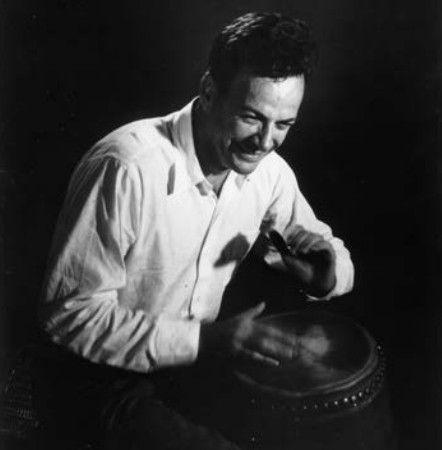
\includegraphics[width=0.4\textwidth]{Chapter0/Feynman}
\end{wrapfigure}
这是我前年与去年在加利福尼亚理工学院对一二年级学生讲授物理学的讲义。当然,这本讲义并不是课堂讲授的逐字逐句记录,而是已经经过了编辑加工,有的地方多一些,有的地方少一些。我们的课堂讲授只是整个课程的一部分。全班180个学生每周两次聚集在大教室里听课,然后分成15到20人的小组在助教辅导下进行复习巩固。此外,每周还有一次实验课。

在这些讲授中,我们想要抓住的特殊问题是,要使充满热情而又相当聪明的中学毕业生进入加利福尼亚理工学院后仍旧保持他们的兴趣。他们在进入学院前就听说过不少关于物理学是如何有趣以及如何引人入胜——相对论、量子力学以及其他的新概念。但是,一旦他们学完两年我们以前的那种课程后,许多人就泄气了,因为教给他们意义重大、新颖的现代的物理概念实在太少。他们被安排去学习像斜面、静电学以及诸如此类的内容,两年过去,没什么收获。问题在于,我们是否有可能设置一门课程能够顾全那些比较优秀的、兴致勃勃的学生,使其保持求知热情。
      
我们所讲授的课程丝毫也不意味着是一门概况性的课程,而是极其严肃的。我想这些课程是对班级中最聪明的学生而讲的,并且可以肯定,这可能是对的,甚至最聪明的学生也无法完全消化讲课中的所有内容——其中加入了除主要讨论的内容之外的有关思想和概念多方面应用的建议。不过,为了这个缘故,我力图使所有的陈述尽可能准确,并在每种场合都指明有关的方程式和概念在物理学的主体中占有什么地位,以及--随着他们学习深入——应怎样作出修正。我还感到,重要的是要向这样的学生指出,他们应能理解——如果他们够聪明的话-—哪些是从已学过的内容中推演出来的,哪些是作为新的概念而引进的。当出现新的概念时,假若这些概念是可推演的,我就尽量把它们推演出来,否则就直接说明这星一个新的概念,它根本不能用已学过的东西来阐明,也不可能予以证明,而是直接引进的。
      
在讲授开始时,我假定学生们在中学已学过一些内容,如几何光学、简单的化学概念,等等。我也看不出有任何理由要按一定的次序来讲授。就是说没有详细讨论某些内容之前,不可以提到这些内容。在讲授中,有许多当时还没有充分讨论过的内容出现。这些内容比较完整的讨论要到以后学生的预备知识更齐全时再进行。电感和能级的概念就是例子,起先,只是以非常定性的方式引入这些概念,后来再进行较全面的讨论。
      
在针对那些较积极的学生的同时,我也要照顾到另一些学生,对他们来说,这些外加的五彩缤纷的内容和不重要的应用只会使其感到头痛,也根本不能要求他们掌握讲授中的大部分内容。对这些学生而言,我要求他们至少能学到中心内容或材料的脉络。即使他不理解一堂课中的所有内容,我希望他也不要紧张不安。我并不要求他理解所有的内容,只要求他理解核心的和最确切的面貌。当然,对他来说也应当具有一定的理解能力,来领会哪些是主要定理和主要概念,哪些则是更高深的枝节问题和应用,这些要过几年他才会理解。

在讲课过程中有一个严重困难:在课程的讲授过程中一点也没有学生给教师的反馈来指示讲授的效果究竟如何。这的确是一个很严重的困难,我不知道讲课的实际效果的好坏。整个事件实质上是一种实验。假如要再讲一次的话,我将不会按同样的方式去讲——我希望我丕会再来一次!然而,我想就物理内容来说,第一年的情形看来还是十分满意的。
  
但在第二年,我就不那么满意了。课程的第一部分涉及电学和磁学,我想不出什么真正独特的或不同的处理方法,也想不出什么比通常的讲授方式格外引人入胜的方法。因此在讲授电磁学时,我并不认为自己做了很多事情。在第二年末,我原来打算在电磁学后再多讲一些物性方面的内容,主要讨论这样一些内容如基本模式、扩散方程的解、振动系统、正交函数等等,并且阐述通常称为“数学物理方法”的初等部分内容。回顾起来,我想假如再讲一次的话,我会回到原来的想法上去,但由于没有要我再讲这些课程的打算,有人就建议介绍一些量子力学——就是你们将在第3卷中见到的——或许是有益的。
  
显然,主修物理学的学生们可以等到第三年学量子力学。但是,另一方面,有一种说法认为许多听我们课的学生是把学习物理作为他们对其他领域的主要兴趣的背景;而通常处理量子力学的方式对大多数学生来说这些内容几乎是无用的,因为他们必须花费相当长的时间来学习它。然而,在量子力学的实际应用中——特别是较复杂的应用中,如电机工程和化学领域内--微分方程处理方法的全部工具实际上是用不到的。所以,我试图这样来描述量子力学的原理,即不要求学生首先掌握有关偏微分方程的数学。我想,即使对一个物理学家来说,我想试着这样做--按照这种颠倒的方式来介绍量子力学——是一件有趣的事,由于种种理由,这从讲课本身或许会明白。不过我认为,在量子力学方面的尝试不是很成功,这主要是因为在最后我实际上已没有足够的时间(例如,我应该再多讲三四次来比较完整地讨论能带、概率幅的空间的依赖关系等这类问题)。而且,我过去从未以这种方式讲授过这部分课程,因此缺乏来自学生的反馈就尤其严重了。我现在相信,还是应当迟一些讲授量子力学。或许有一天我会有机会再来讲授这部分内容,到那时我将会讲好它。
  
在这本讲义中没有列入有关解题的内容,这是因为另有辅导课。虽然在第一年中,我的确讲授过三次关于怎样解题的内容,但没有将它们收在这里。此外,还讲过一次惯性导航,应该在转动系统后面,遗憾的是在这里也略去了。第五讲和第六讲实际上是桑兹讲授的,那时我正外出。
  
当然,问题在于我们这个尝试的效果究竟如何。我个人的看法是悲观的,虽然与学生接触的大部分教师似乎并不都有这种看法。我并不认为自己在对待学生方面做得很出色。当我看到大多数学生在考试中采取的处理问题的方法时,我认为这种方式是失败了。当然,朋友们提醒我,也有一二十个学生——非常出人意外地——几乎理解讲授的全部内容,并且非常积极地攻读有关材料,兴奋地、感兴趣地钻研许多问题。我相信,这些学生现在已具备了一流的物理基础,他们毕竟是我想要培养的学生。但是,“教育之力量鲜见成效,除非施之于天资敏悟者,然若此又实为多余。”[吉本(Gibbon) \footnote{Edward Gibbon (1737 - 1794),英国历史学家。————译者注} ]
  
但是,我并不想使任何一个学生完全落在后面,或许我曾经这样做的。我想,我们能够更好地帮助学生的一个办法是,多花一些精力去编纂一套能够阐明讲课中的某些概念的习题。习题能够充实课堂讲授,使讲过的概念更加实际,更加完整和更加易于牢记。

然而,我认为要解决这个教育问题就要认识到最佳的教学只有当学生和优秀的教师之间建立起个人的直接关系在这种情况下,学生可以讨论概念、考虑问题、谈论问题,除此之外,别无他法。仅仅坐在课堂里听课或者只做指定的习题是不可能学到许多东西的。但是,现在我们有这么多学生要教育,因此我们必须尽量找出一种代替理想情况的办法。或许,我的讲义可以作出一些贡献;也许在某些小地方有个别教师和学生会从讲义中受到一些启示或获得某些观念,当他们彻底思考讲授内容,或者进一步发展其中的一些想法时,他们或许会得到乐趣。

\hfill R.P.费曼

\hfill 1963年6月

\chapter*{前言}

本书是根据R. P.费恩曼教授在加利福尼亚理工学院1961-1962学年所讲物理学导论课编写的,它包括全校一二年级学生念的两年导论课的第一年的内容,在1962-1963学年还继续讲授了这门课程的第二年的内容。这些讲授构成四年来对导论课所作的根本性修改的主要部分。
  
课程要进行彻底的修改,不但是由于近数十年来物理学迅速发展的需要,而且还有鉴于高中数学课内容改进后,入校新生的数学能力有了稳步的提高。我们希望利用有利的条件,并且希望能在课程中介绍足够的现代题材,从而使这门课程能引起学生的注意和兴趣,并能体现出现代物理的状况。
  
在应当包括哪些内容以及怎样介绍这些内容方面,为了能形成各种想法,我们鼓励物理系的许多教师以提纲的形式对课程的修改提出意见。人们对其中的几种想法进行了详细的讨论和评述。大家几乎立即同意,认为仅仅换一本教科书或者重新写一本教科书,是不可能完成对这门课程的彻底修改的。新的课程应当以每周讲二三次的一系列讲授为,中心,而随着课程的进展,相应的教材内容将作为其从属的工作而产生出来,在讲课的同时,也要安排适当的实验来配合讲授内容。据此提出了课程的初步轮廓。但大家也认识到,这是不完全的和试验性的,有待于实际承担讲授工作的人作出相当大的修改。
  
关于最后究竟以什么方式来实施这门课程,大家考虑过几种方案。这些方案大多类似,由N个人进行合作,均匀地分担责任,即每个人负责 1/N 的材料,进行讲授,并使他这部分成文。然而,由于没有足够的教师,同时因为参加者的个性与哲学见解不同,很难保持一致的观点。因此这种方案看来难以实现。
  
桑兹教授令人鼓舞的想法是他领悟到,我们实际上所拥有的能力不只是可以建立一门新的、不同的物理课程,而且有可能创立一门完全独特的课程。他建议由费恩曼教授来准备和进行讲授,并用磁带录音。再将这些录音抄写出来并加以编辑,就成为新课程的教科书了。我们所采用的基本上就是这样的方案。
  
起先我们估计必要的编辑工作不会很多,大体上只是一些补充图画、核对标点、语法之类的事,完全可以由一两个研究生花部分时间去完成。遗憾的是我们很快就发现这种估计是不正确的。事实上,即使对题材不进行重新组织或修改(有时这是必要的),只是把逐字逐句的记录改写成可供阅读的形式,就需要相当多的编辑工作。而且,这不是一个技术编辑或一个研究生就能办得了的事,而是需要一位专业物理工作者对每次讲授的内容专心一致地花上10-20小时才行!
  
编辑任务的艰巨,再加上要尽快把材料发给学生,这就大大地限制了对材料所能作出的推敲润色工作。因此,我们只能指望完成一本初步的、但专业上保持正确的、立即可以使用

\hfill R.P.费曼

\hfill 1963年7月

\shorttoc{目录}{0}

\renewcommand*\contentsname{详细目录}
\setcounter{tocdepth}{2}
\tableofcontents

\newpage

\pagenumbering{arabic}
\setcounter{page}{1}

\chapter{原子的运动}

\section{引言}

这是一门两学年的物理课,我们开设这门课程是着眼于你们,读者们,将成为物理学工作者。当然,情况并非一定如此,但是每门学科的教授都是这样设想的!假如你打算成为一个物理学工作者,就要学习很多东西;这是一个200年以来空前蓬勃发展的知识领域。事实上,你会想到,这么多的知识是不可能在四年内学完的,确实不可能;你们还得到研究院去继续学习。

相当出人意外的是,尽管在这么长时间中做了极其大量的工作,但却有可能把这一大堆成果大大地加以浓缩。 这就是说,找到一些概括我们所有知识的\uwave{定律}。 不过,即使如此,掌握这些定律也是颇为困难的.。因此在你对科学的这部分与那部分题材之间的关系还没有一个大致的了解之前就让你去钻研这个庞大的课题的话,就不公平了。根据这种看法,前三章将略述物理学与其他科学的关系,各门学科之间的相互联系以及科学的含义,这有助于你们对本学科产生一种切身的感受。

你们可能会问,在讲授欧几里德几何时,先是陈述公理,然后作出各种各样的推论,那为什么在讲授物理学时不能先直截了当地列出基本定律, 然后再就一切可能的情况说明定律的应用呢?(这样一来,如果你不满足于要花四年时间来学习物理,那你是否打算在4分钟内学完它?)我们不能这样做是由于两个理由。 第一,我们还\uwave{不知道}所有的基本定律:未知领域的边界在不断地扩展; 第二,正确地叙述物理定律要涉及到一些非常陌生的概念,而叙述这些概念又要用到高等数学。因此,即使为了知道\uwave{词}的含义,也需要大量的预备性的训练。的确,那样做是行不通的,我们只能一步一步地来。

大自然整体的每一部分始终只不过是对于整个真理——或者说,\uwave{对于}我们至今所了解的\uwave{整个真理}——的\uwave{逼近}。实际上,人们知道的每件事都只是某种近似,因为\uwave{我们懂得},到目前为止,我们\uwave{确实还不知道所有的定律}。因此,我们之所以需要学习一些东西,正是为了要抛弃以前的谬见,或者更可能的是为了改正以前的谬见。

科学的原则——或者简直可称为科学的定义为:实验是\uwave{一切知识的试金石},实验是科学“真理”的唯一\uwave{鉴定者}。 但是什么是知识的源泉呢?那些要检验的定律又是从何而来的?从某种意义上说,实验为我们提供了种种线索,因此可以说是实验本身促成了这些定律的产生。但是,要从这些线索中作出重大的判断,还需要有丰富的想象力去对蕴藏在所有这些线索后面的令人惊讶、简单、而又非常奇特的图象进行猜测,然后,再用实验来验证我们的猜测究竟对不对。这个想像过程是很艰难的,因此在物理学中有所分工,\uwave{理论}物理学家进行想象、推演和猜测新的定律,但并不做实验;而\uwave{实验}物理学家则进行实验、想象、推演和猜测。

我们说过,自然的定律是近似的:起先我们找到的是“错”的定律,然后才发现“对”的定律。那么,一个实验怎么可能是“错误”的呢?首先,通常是:仪器上有些毛病,而你又没有注意,但是这种问题是容易确定的,可以反复检查。如果不去纠缠在这种次要的问题上,那么实验的结果怎么\uwave{可能}是错误的呢?这只可能是由于不够精确罢了。例如,一个物体的质量似乎是从来不变的,转动的陀螺与静止的陀螺一样重。结果就发现了一条“定律”:质量是个常数,与速率无关。然而现在发现这条“定律”却是不正确的。质量实际上随著速度的加大而增加,但是要速度接近光速,才会显著增加。\uwave{正确}的定律是:如果一个物体的速率小于100海里/秒,那么它的质量的变化不超过百万分之一,在这种近似形式下,这就是一条正确的定律。因此,人们可能认为新的定律实际上并没有什么有意义的差别。当然,这可以说对,也可以说不对。对于一般的速率我们当然可以忘掉它,而用简单的质量守恒定律作为一种很好的近似。但是对于告诉情况这就不正确了:速率越高,就越不正确。

最后,最有趣的是,\uwave{就哲学上而言},使用近似的定律是\uwave{完全错误}的。纵然质量的变化只是一点点,我们的整个世界图景也得改变。这是有关在定律后面的哲学或基本观念的一件十分特殊的事,即使是极小的效应有时在我们的观念上也要引起深刻的变化。

那么,我们应该首先教什么呢?是否应先教那些\uwave{正确}的、陌生的定律以及有关的奇特而困难的观念,例如相对论,四维时空等等之类?还是应先教简单的“质量守恒”定律,即那条虽然只是近似的,但并不包含那种困难的观念的定律?前一条定律比较引人入胜,比较奇特和比较有趣,但是后一条定律在开始时比较容易掌握,它是真正理解前一种观念的第一步。这个问题在物理教学中会一再出现,在不同的时候,我们将要用不同的方式去解决它。但是在每个阶段都值得去弄明白:我们现在所知道的是什么,它的正确性如何,它怎样适应其他的各种事情,以及当我们进一步学习后它会有怎样的变化。

让我们按照我们所理解的当代科学(特别是物理学,但是也包括周围有关的其他科学)的轮廓继续讲下去,这样,当我们以后专门注意某些特殊问题时,就会对于背景情况有所了解——为什么这些特殊问题是有趣的,它们又是怎样适应整体结构的。

那么,我们世界的总体图象是怎样的呢?

\section{物质是原子构成的}

假如由于某种大灾难,所有的科学知识都丢失了,只有一句话传给下一代,那么怎样才能用最少的词汇来表达最多的信息呢?我相信这句话是原子的假设(或者说原子的事实,无论你愿意怎样称呼都行): 所有的物体都是用原子构成的——这些原子是一些小小的粒子,它们一直不停地运动着。 当彼此略微离开时相互吸引, 当彼此过于挤紧时又互相排斥。只要稍微想一下,你就会发现,在这一句话中包含了大量的有关世界的信息。

\begin{wrapfigure}{r}{0.4\textwidth}
    \centering
    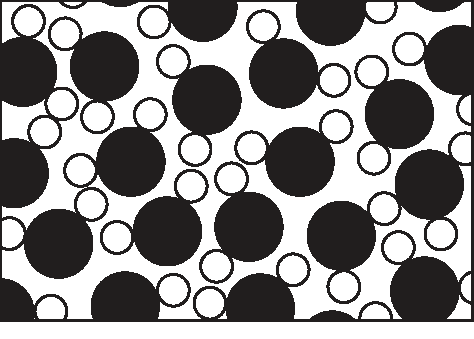
\includegraphics[width=0.35\textwidth]{Chapter1/放大10亿倍的水}
    \caption{放大10亿倍的水}
    \label{figure:放大10亿倍的水}
\end{wrapfigure}
为了说明原子观念的重要作用,假设有一滴直径为1/4英寸的水滴,即使我们非常贴近地观察,也只能见到光滑的、连续的水,而没有任何其他东西并且即使我们用最好的光学显微镜(大致可放大2000倍)把这滴水放大到40英尺左右(相当于一个大房间那大),然后再靠得相当近地去观察,我们所看到的仍然是比较光滑的水,不过到处有一些足球状的东西在来回游动,非常有趣。这些东西是草履虫。你们可能就到此为止,对草履虫以及它的摆动的纤毛和卷曲的身体感到十分好奇。也许除了把草履虫放得更大一些,看看它的内部外,就不再进一步观察了。当然这是生物学的课题,但是现在我们继续观察下去,再把水放大2000倍更接近地观察水这种物质本身。这时,水滴已放大到有15英里那样大了,如果你再十分贴近地观察,你将看到水中充满了某种不再具有光滑外表的东西,而是有些象从远处看过去挤在足球场上的人群。

为了能看出挤满的究竟是些什么东西,我们再把它放大250倍后就会看到某种类似于图\ref{figure:放大10亿倍的水}所示的情形。这是放大了10亿倍的水的图象,但是在以下这几方面是理想化了的。首先,各种粒子用简单的方式画成有明显的边缘,这是不精确的。其次,为了简便起见,把它们都画成二维的排列,实际上它们当然是在三维空间中运动的。注意在图中有两类“斑点”或圆,它们各表示氧原子(黑色)和氢原子(白色),而每个氧原子有两个氢原子和它联结在一起(一个氧原子与两个氢原子组成的一个小组称为一个分子)。图象中还有一个被理想化的地方是自然界中的真实粒子总是在不停地跳动,彼此绕来绕去地转着,因而你必须把这幅画面想象成能动的而不是静止的。另一件不能在图上说明的事实是粒子为“粘在一起”的,它们彼此吸引着,这个被那个拉住等等,可以说,整个一群“胶合在一起”,另一方面,这些粒子也不是挤到一块儿,如果你把两个粒子挤得很紧,它们就互相推斥。

\begin{wrapfigure}{r}{0.3\textwidth}
    \centering
    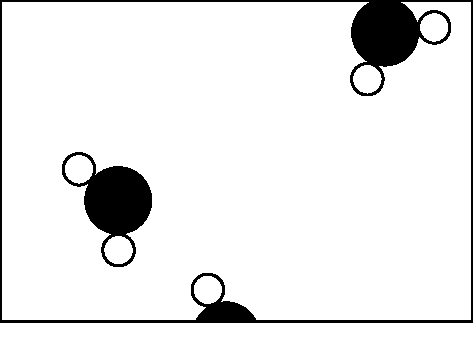
\includegraphics[width=0.25\textwidth]{Chapter1/水蒸气}
    \caption{水蒸气}
    \label{figure:水蒸气}
\end{wrapfigure}
原子的半径约为$1\sim2\times10^{-8}$厘米,$ 10^{-8} $厘米现在称为1Å(这只是另一个名称),所以我们说原子的半径为$1\sim2$\r{A},另一个记住原子大小的方法是这样的:如果把苹果放大到地球那样大,那么苹果中的原子就差不多有原来的苹果那样大。

现在,想象这个大水滴是由所有这些跳动的粒子一个挨一个地“粘合”起来的,水能保持一定的体积而并不散开,因为它的分子彼此吸引。 如果水滴在一个斜面上,它能从一个位置移动到另一个位置。水会流动,但是并不会消失——它们并没有飞逝,因为分子之间有吸引力。这种跳动就是我们所说的热运动,当温度升高时,这种运动就增强了。如果我们加热水滴,跳动就增加,原子之间的空隙也增大。如果继续加热到分子间的引力不足以将彼此拉住时,它们就分开来飞散了。当然,这正是我们从水制取水蒸气的方法——提高温度,粒子由于运动的增强而飞散。图\ref{figure:水蒸气}是一幅水蒸气的图象。这张水蒸气图象有一个不足之处:在通常的气压下在整个房间里只有少数几个分子,决不可能在这样一张图象中有三个以上的分子。在大多数情况下,这样大小的方块中可能连一个都不会有——不过碰巧在这张图中有两个半或三个分子(只有这样图象才不会是完全空白的)。现在比起水来,在水蒸气的情况下,我们可以更清楚地看到水所特有的分子。为了简单起见,将分子画成具有120°的夹角,实际上,这个角是105°3′,氢原子中心与氧原子中心之间的距离是0.957Å。这样看来,我们对这个分子了解得很清楚了。

\begin{wrapfigure}{l}{0.25\textwidth}
    \centering
    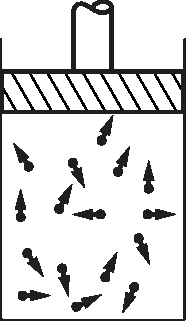
\includegraphics[width=0.2\textwidth]{Chapter1/一个配有活塞的汽缸}
    \caption{汽缸}
    \label{figure:一个配有活塞的汽缸}
\end{wrapfigure}
让我们来看一下,水蒸气或任何其他气体具有一些什么性质。这些气体分子是彼此分离的,它们打在墙上时,会反弹回来。设想在一个房间里有一些网球(100个左右)不断地来回跳动,当它们打到墙上后,就将墙推离原位(当然,我们必须将墙推回去)。这意味着气体施加一个“颤动”的力,而我们的粗糙的感官(并没有被我们自己放大十亿倍)只感到一个平均的推力。为了把气体限制在一定的范围之内,我们必须施加一个压力。图\ref{figure:一个配有活塞的汽缸}是一个盛气体的标准容器(所有教科书中都有这种图)一个配有活塞的汽缸,由于不论水分子的形状如何,情况都是一样,因此为简单起见,我们把它们画成网球形状或者小黑点。这些东西沿着所有的方向不停地运动着。由于有这么多的气体分子一直在撞击顶端的活塞,因此要使活塞不被这种不断的碰撞逐渐顶出来必须施加一定的力把活塞压下去,这个力称为\uwave{压力}(实际上,是压强乘以面积)。很清楚,这个力正比于面积,因为如果我们增大面积而保持每立方厘米内的分子数不变的话,那么分子与活塞碰撞次数增加的比例与面积增加的比例是相同的。

现在让我们在这个容器内放入两倍的分子,以使密度增加一倍,同时让它们具有同样的速度,即相同的温度。那么,作为一种很好的近似,碰撞的次数也将增加一倍,由于每次碰撞仍然和先前那样“有力”,压力就正比于密度。如果我们考虑到原子之间的力的真实性质,那么由于原子之间的吸引,可以预期压力略有减少;而由于原子也占有有限的体积,则可以预期压力略有增加。无论如何,作为一个很好的近似,如果原子较少,密度足够低,那么,\uwave{压力正比于密度}。

我们还可以看一下其他情况。如果提高温度而不改变气体密度,亦即只增加原子的速度,那么在压力上会出现什么情况?当然,原子将撞击得更剧烈一些,因为它们运动得更快一些。此外,它们的碰撞更频繁了,因此压力将增加,你们看,原子理论的概念是多么简单!

我们来考虑另一种情况,假定活塞向下移动,原子就慢慢地被压缩在一个较小的空间里。当原子碰到运动着的活塞时,会发生什么情况呢?很显然,原子由于碰撞而提高了速率,例如,你可以试一下乒乓球从一个朝前运动的球拍弹回来时的情况,你会发现弹回的速率比打到球拍上的速率更大一些(一个特例是如果一个原子恰好静止不动,那么在活塞碰上它以后,当然就运动了)。这样原子在弹离活寒时比碰上去之前更“热”因此所有容器中的分子的速率都提高了。这意味着,\uwave{当我们缓慢压缩气体时,气体的温度会升高}。结果,在缓慢压缩时,气体的温度将升高;而在缓慢膨胀时,气体的温度将降低。

\begin{wrapfigure}{r}{0.35\textwidth}
    \centering
    \includegraphics[width=0.3\textwidth]{Chapter1/冰}
    \caption{冰}
    \label{figure:冰}
\end{wrapfigure}
现在回到我们的那滴水上去,从另一个角度去观察一下,假定现在降低水滴的温度,并且假定水的原子、分子的跳动逐渐减小。我们知道在原子之间存在着引力,因而过一会儿,它们就不能再跳得那么厉害了。图\ref{figure:冰}表示在很低的温度下会出现什么样的情况。这时分子连接成一种新的图象,这就是冰。这个特殊的冰的图象是不正确的,因为它只是二维的,但是它在定性上是正确的。有趣的一点是,\uwave{对于每一个原子,都有它的确定位置}。你们可以很容易地设想,如果我们用某种方式使冰的一端的所有的原子按一定的方式排列,并让每个原子处在一定的位置上,那么由于互相连接的结构很牢固,几英里之外(在我们放大的比例下)的另一端也将有确定的位置。如果我们抓住一根冰棍的一端,另一端就会阻止我们把它拉出去。这种情况不象水那样由于跳动加强以致所有的原子以种种方式到处跑来跑去, 因而结构也就被破坏了。固体与液体的差别就在于:在固体中,原子以某种称为\uwave{晶体排列}的方式排列着,即使在较长的距离上它们的位置也不能杂乱无章。晶体一端的原子位置取决于晶体另一端的与之相距千百万个原子的排列位置。图\ref{figure:冰}是一种虚构的冰的排列状况,它虽然包括了冰的许多正确的特征,但并不是真实的排列情况。正确的特征之一是这里具有一种六边形的对称性。你们可以看到:如果把画面绕一根轴转动120°的话,它仍然回到原来的形状,因此,在冰里存在着一定的对称性,这说明为什么雪花具有六边形的外表。从图\ref{figure:冰}中还可以看到为什么冰融解时会缩小。在这里列出的冰的晶体图样中有许多“孔”,真实的冰的结构也是如此,在排列打散后,这些孔就可以容纳分子。除水和铅字合金\footnote{铅、锑、锡的合金,也称为活字合金。}外,许多简单的物质在融解时都要膨胀,因为在固体的晶体结构中,原子是密集堆积的,而当熔解时,需要有更多的空间供原子活动,但是敞形结构则会倒坍,体积反而收缩了,就象水的情况那样。

虽然冰有一种“刚性的”结晶形态,它的温度也会变化——冰也储存热量,如果我们愿意的话,就可以改变热量的储存。对冰来说,这种热量指的是什么呢?冰的原子并不是静止不动的,它们不断地摇晃着、振动着,所以虽然晶体存在着一种确定的次序——一种确定的结构,所有的原子仍都“在适当的位置”上振动,当我们提高温度时,它们振动的幅度就越来越大,直到离开原来的位置为止。我们把这个过程称为熔解,当降低温度时,振动的幅度越来越小,直到绝对零度原子仍能有最低限度的振动,而\uwave{不是停止}振动。原子所具有的这种最低的振动不足以使物质熔解,只有一个例外,即氦。在温度降低时,氦原子的运动只是尽可能地减弱,但即使在绝对零度时也有足够的运动使之不致于凝固,除非把压力加得这样大以致将原子都挤在一起。如果我们提高压力,就可以使它凝固。

\section{原子过程}

\begin{wrapfigure}{r}{0.4\textwidth}
    \centering
    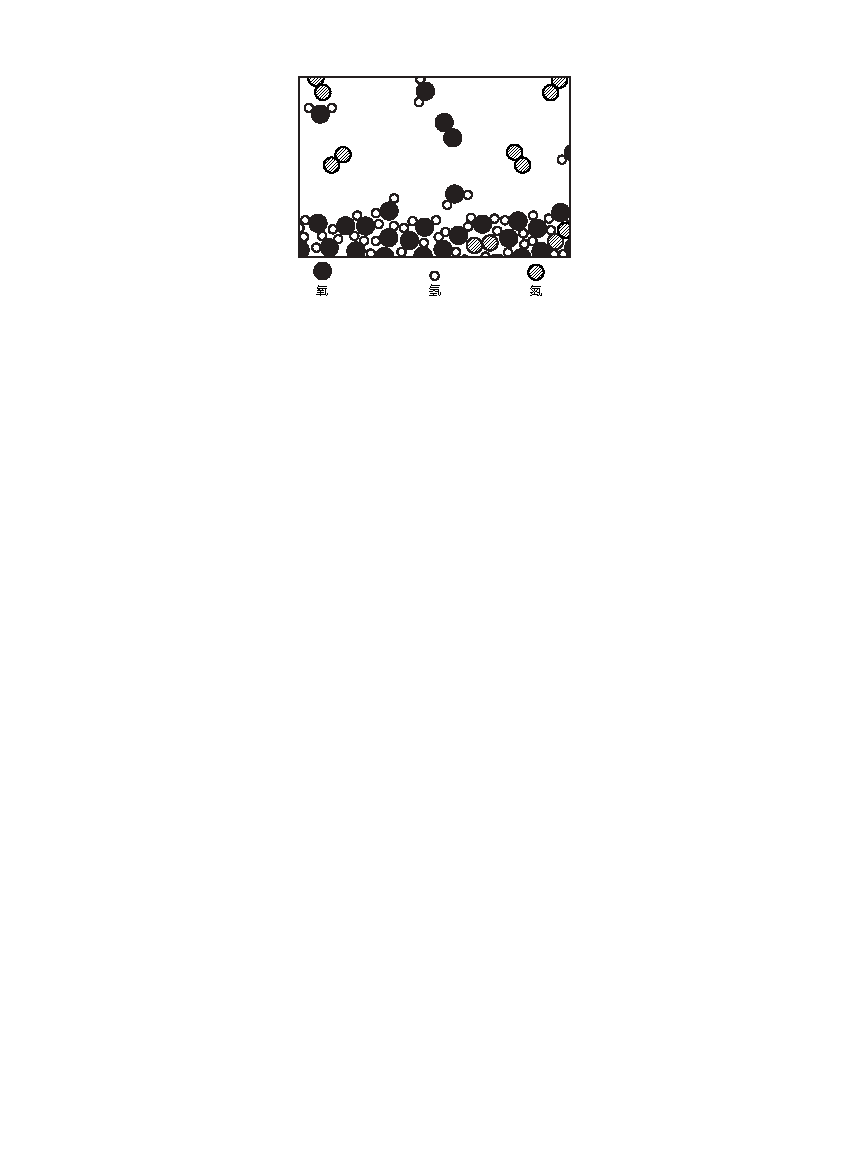
\includegraphics[width=0.35\textwidth]{Chapter1/空气中水的蒸发}
    \caption{空气中水的蒸发}
    \label{figure:空气中水的蒸发}
\end{wrapfigure}
关于从原子的观点来描写固体、液体和气体,我们就讲到这里。然而原子的假设也可以描写\uwave{过程},所以我们现在从原子的观点来考察一些过程。我们要考察的第一个过程与水的表面有关。在水的表面有些什么情况呢?设想水的表面上是空气,现在我们来把图画得更复杂一些——也更实际一些,如图\ref{figure:空气中水的蒸发}所示。我们看到,水分子仍然象先前那样,组成大量的水,但现在还看到水的表面。在水面上我们发现一些东西:首先,水面上有水的分子,这就是\uwave{水的蒸气},在水面上总是有水蒸气的。(在水蒸气与水之间存在着一种平衡,这种平衡我们以后再讲。)此外,我们还发现一些别的分子:这里是两个氧原子彼此结合在一起组成一个\uwave{氧分子},那里是两个氮原子结合在一起组成一个氮分子。空气几乎完全是由氮气、氧气、水蒸气组成的,此外还有少量的二氧化碳、氩气和其他一些气体。所以在水面上的是含有一些水蒸气的气体。那么在这种情况下会发生什么事呢?水里的分子不断地晃来晃去。有时,在水面上有个别分子碰巧受到比通常情况下更大的冲击而被“踢”出表面。因为图\ref{figure:空气中水的蒸发}是\uwave{静止}的画面,所以在图上难以看出所发生的事。但是我们可以想象表面附近的某一个分子刚好受到碰撞而飞了出去,或者也许另一个分子也受到碰撞而飞了出去。分子一个接着一个地跑了出去,水就消失了——蒸发了。但是如果把容器盖上,过了一会儿就会发现在空气分子中有大量的水分子。水蒸气的分子不时地飞到水面,又回到水中。结果,我们看到那个看来死气沉沉的、无趣的事情——杯盖上的可能已放了二十年的水——实在包含了一直生气勃勃而有趣的现象。对我们这双肉眼而言,看不出有任何变化,但是如果能放大十亿倍来看的话,我们就能发现情况一直在变化,一些分子离开水面,又一些分子则回到了水面。

为什么\uwave{我们看不出变化呢}?因为有多少分子离开水面就会有多少分子回到水面!归根到底“没有任何事情发生”如果现在我们把容器盖打开,使潮湿的空气吹走而代之以干燥空气,那么离开水面的分子数还是如先前那样多,因为这只取决于水分子晃动的程度,但是回到水面的分子数则大大地减少了,因为在水面上的水分子数已极其稀少。因此逸出水面的分子比进入水面的分子多,水就蒸发了。所以,如果你要使水蒸发的话,就打开风扇吧!

这里还有另一件事情:哪些分子会离开?一个分子能离开水面是由于它偶然比通常情况稍微多积累了一些能量,这样才能使它摆脱邻近分子的吸引。结果,由于离开水面的分子带走的能量比平均能量大,留在水中的分子的运动平均起来就比先前\uwave{减弱}。因此液体蒸发时会逐渐冷却。当然,当一个水蒸气分子从空气中跑向水面时,它一靠近水面就要突然受到一个很强的吸引。这就使它进入水中时具有更大的速度,结果就产生热量。所以当水分子离开水面时,它们带走了热量;而当它们回到水面时, 则产生了热量。当然,如果不存在净的蒸发现象的话,什么结果也不会发生——水的温度并不改变。如果我们向水面上吹风,使蒸发的分子数一直占优势,水就会冷却。因此,要使汤冷却就得不停地吹!

当然,你们应当了解,刚才所说的那个过程实际上要比我们所指出的更为复杂。不仅水分子进入空气,不时还有氧分子或氮分子跑到水里,“消失”在一大堆水分子中,这样空气就溶解在水中了。氧和氮的分子进入水中,水里就含有空气。如果我们突然从容器中抽走空气,那么空气分子出来要比进去来得快,这样就形成了气泡。你们可能知道,这对潜水员是很不利的。

\begin{wrapfigure}{r}{0.4\textwidth}
    \centering
    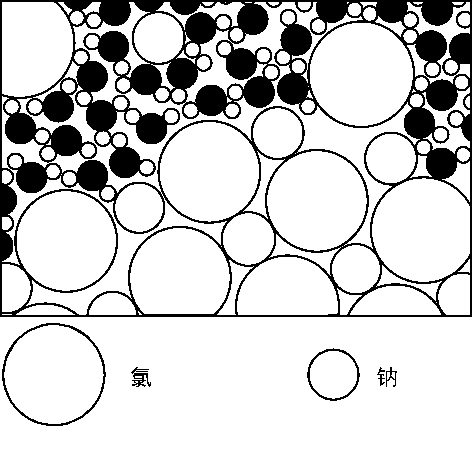
\includegraphics[width=0.35\textwidth]{Chapter1/盐在水中的溶解}
    \caption{盐在水中的溶解}
    \label{figure:盐在水中的溶解}
\end{wrapfigure}
现在我们来考虑另一种过程。在图\ref{figure:盐在水中的溶解}中,我们从原子的观点来看固体在水中溶解。如果我们把结晶盐粒丢入水中,会出现什么情况呢?食盐是一种固体,也是一种晶体,并且是“食盐原子”的有规则的排列。

严格地说, 这种晶体不是用原子而是用我们所谓的\uwave{离子}构成的!离子就是带有额外电子的原子,或失去一些电子的原子。在食盐晶体中我们发现了氯离子(带有一个额外电子的氯原子)和钠离子(失去一个电子的钠原子)。在固态食盐中,所有的离子都由于电的作用而吸引在一起,但是当我们把食盐投到水里后,就会发现,所有的离子都由于电的作用而吸引在一起,有一些离子离散了。在图\ref{figure:盐在水中的溶解}中有一个氯离子松开来了,其他的原子则以离子的形式在水中浮动。这张图画得相当仔细:例如,注意水分子中的氢原子一端大多靠近氯离子,而在钠离子周围所见到的大多是氧原子的那一端,因为钠是正的,而水的氧原子一端是负的,它们之间有电的吸引。我们能不能从这幅图画中看出盐究竟是\uwave{溶解于}水中,还是从水中\uwave{结晶出来}?当然,我们看不出来,因为当某些原子离开晶体时,另一些原子又重新聚集到晶体上。整个过程是一个\uwave{动态过程},犹如同蒸发的情况,它取决于水中盐的含量是超过还是少于形成平衡所需要的数量。所谓平衡我们指的是这种情况,即原子离开晶体的比率正好与回到晶体的比率相同。假如在水中几乎没有什么盐,离开的原子就比回去的原子多,食盐就溶解。但另一方面,如果水里的“食盐原子”太多,那么回去的就多于离开的,食盐就结晶。

\begin{figure}
    \centering
    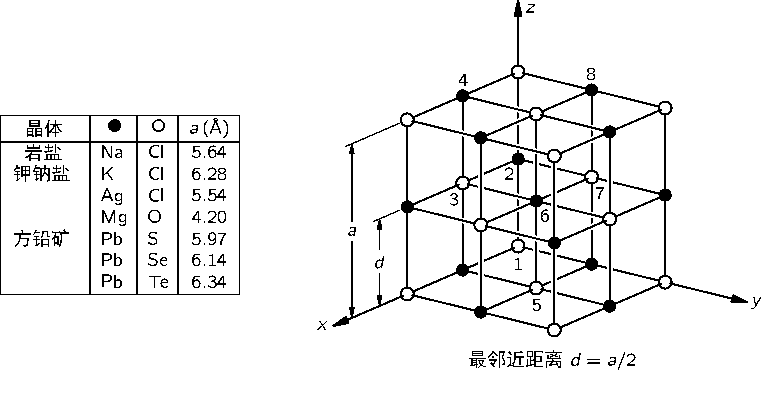
\includegraphics[width=0.65\textwidth]{Chapter1/食盐的晶体结构}
    \caption{食盐的晶体结构}
    \label{figure:食盐的晶体结构}
\end{figure}

我们顺便说一下,物质的分子这个概念只是近似的,而且只是对某些种类的物质才有意义。很清楚,在水的情况下,三个原子彼此确实站在一起。但是在固体的氯化钠情况下就不那么明确了。在氯化钠中钠离子和氯离子只是以立方体的形式排列。这里没有一种把它们自然分成“食盐分子”的方式。

现在回到我们的溶解与淀积的讨论上。如果增加食盐溶液的温度,那么原子离开的比率就会增加,而原子回来的比率也会增加。结果是一般很难预言会朝哪一个方向发展,固体溶解得多一些还是少一些。当温度提高时,大多数物质更易溶解, 但是某些物质则更不易溶解。

\section{化学反应}

\begin{wrapfigure}{r}{0.35\textwidth}
    \centering
    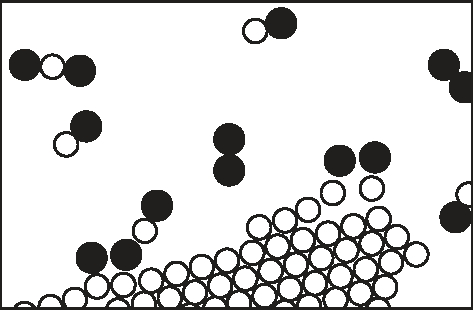
\includegraphics[width=0.3\textwidth]{Chapter1/碳在氧气中的燃烧}
    \caption{碳在氧气中的燃烧}
    \label{figure:碳在氧气中的燃烧}
\end{wrapfigure}
到现在为止,在我们所描述的一切过程中,原子和离子的伙伴并没有变更,但是当然也有这种情况,原子的组合的确改变了,形成新的分子。图\ref{figure:碳在氧气中的燃烧}就是说明这一情况的。在一个过程中如果原子的伙伴重新排列,我们就称之为\uwave{化学反应}。其他前面所描述的过程称为物理过程,但是二者之间并没有明显的界限(大自然并不关心我们究竟如何去称呼,她只知道不断地进行工作)。图\ref{figure:碳在氧气中的燃烧}表示碳在氧气中的燃烧。在氧气中,\uwave{两个}氧原子紧紧地吸引在一起(为什么不是\uwave{三个}甚至四个吸引在一起?这是此类原子过程的一个很典型的特征。原子是非常特别的:它们喜欢一定的伙伴,一定的方向,等等。物理学的任务就是要分析每一个原子为什么想要它所希望要的东西。无论如何,两个氧原子形成了一个饱和的、适宜的分子。)

这些碳原子应该处于固态晶体之中(可以是石墨,也可以是金刚石)现在,比如说有一个氧分子跑到碳这边来,每个氧原子可以抓住一个碳原子而以一种新的组合——“碳-氧”——一起飞走,这就是所谓的一氧化碳气体分子,它的化学名称是CO。这种气体分子很简单:字母“CO”实际上就是这个分子的一个画象。但是碳吸引氧的能力比氧吸引氧或者碳吸引碳的能力更大。因此在这个过程中氧原子可能在到达时只带有一点点能量,但是氧和碳的结合却是非常彻底而剧烈的,所有靠近它们的原子都吸收能量。于是就产生了大量的分子运动的能量——动能。当然,这就是燃烧。我们从氧和碳的结合得到了\uwave{热量}。这种热量通常是以热气体的分子运动的形式存在的,但是在某些情况下,由于热量非常大而\uwave{发出了光}。这就是怎样产生火焰的过程。

此外,一氧化碳分子并不感到满足。它可能再缚住另一个氧原子,因此可能出现远为复杂的反应:氧与碳会结合起来,同时偶尔又与一氧化碳分子碰撞。于是一个氧原子可能结合到一个CO分子上,最终形成另一个分子,它包含一个碳原子和两个氧原子,称为二氧化碳,并以\chemfig{CO_2}表示。假如我们以很快的速度在很少的氧气中燃烧碳的话(例如,在汽车引擎中,爆炸是如此迅速,以致没有时间形成二氧化碳),就形成了大量的一氧化碳。在许多这种重新排列的过程中,大量的能量被释放出来,依反应条件的不同而形成爆炸、火焰等等。化学家研究了这些原子的排列情况,发现每一种物质都是某种类型的\uwave{原子的排列}。

为了说明这个概念,我们来考虑另一个例子。如果我们走到一个紫罗兰花圃里去,我们知道那是一种什么香气。这是某种\uwave{分子}或者说原子排列钻进了我们的鼻子。首先,这种分子是怎样钻进来的呢?这很容易。假如香气是飘浮在空气中的某种分子,它们就会到处晃动,四面八方地撞来撞去,很可能偶尔钻进了我们的鼻子。肯定分子并不想特别进入我们的嗅觉器官。在挤成一堆的分子中,大家都无目的地到处徘徊,而碰巧有一些分子却发现自己原来已到达人的鼻子中了

\begin{wrapfigure}{l}{0.4\textwidth}
    \centering
    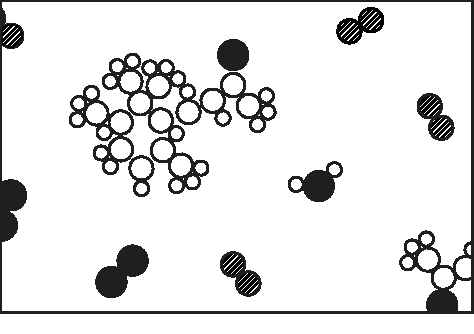
\includegraphics[width=0.35\textwidth]{Chapter1/空气中的紫罗兰香气分子}
    \caption{空气中的紫罗兰香气分子}
    \label{figure:空气中的紫罗兰香气分子}
\end{wrapfigure}
现在,化学家可以取一些象紫罗兰香气这样特殊的分子进行分析,然后告诉我们原子在空间的\uwave{精确排列}。我们知道二氧化碳分子的结构是简单而对称的:\chemfig{O=C=O}。(这也很容易用物理方法来确定。)然而,即使对化学中那些非常复杂的原子队列,人们也可以通过长期的、卓越的探索工作来查明其排列方式。图\ref{figure:空气中的紫罗兰香气分子}是空气中紫罗兰香气图。我们再一次发现有氮、氧以及水蒸气。(为什么这儿有水蒸气?因为紫罗兰是湿的。所有的植物都会蒸发水气。)然而,我们还看到一个由碳原子、氧原子及氢原子组成的“怪物”,它也选择了一种特殊的排列形式。这种形式比二氧化碳的排列远为复杂;事实上,它是一种极为复杂的排列。遗憾的是,我们无法画出所有那些在化学上已确实知道的情况,因为所有的原子的精确排列都是三维的,而我们的画面只是二维的。六个碳原子组成了一个环,但它不是扁平的,而是一种“皱褶”的环。环的所有角度和间距都已知道。所以一个化学式只是这样的分子的一个画象。当一位化学家把它写在黑板上时,粗略地说,他是在二维空间里“画”图。比如,我们见到六个碳原子组成的一个“环”,在一个端点还悬挂着一条碳“链”,链的第二个端点的碳上有一个氧原子,还有三个氢原子连在那个碳原子上,两个氢原子和三个碳原子竖在这儿,等等。

化学家是怎样发现这种排列的呢?他把几瓶东西混合起来,如果变红了,就说明,在某处有两个碳原子与一个氧原子联结在一起;如果变蓝了,就说明根本不是那么一回事。这是所做过的最奇妙的探索工作之一——有机化学。为了发现极其复杂的阵列中的原子排列,化学家观察两种不同的物质混合后究竟会发生什么事?当化学家描述原子的排列时,物理学家从来不怎么相信化学家了解他在谈论的是什么。大约在20年前就能在某些情况下用物理方法来研究这些分子的排列(不完全象我们这个分子那样复杂,只包括了它的一部分),而且能通过\uwave{测量}而不是观察颜色来确定每个原子的位置,嗨!你瞧!化学家几乎总是正确的。

结果,实际上紫罗兰的香气里有三种略为不同的分子,其差别仅在于氢原子的排列不同。

化学的一个任务是给物质命名,从而使我们知道它是什么。给这种形状起个名字看看,这个名称不仅要表明形状,而且还要说出这里是一个氧原子,那里是一个氢原子——确切地说出每 个原子的名称和位置。所以我们可以设想,为了全面起见,化学名称一定是十分复杂的。你们看!这个东西的比较完整的名称是4(2, 2, 3, 6-四甲基-5-环己烯基)-3-丁烯-2-酮,它告诉你这样东西的结构,还告诉你这就是它的排列方式。我们可以意识到化学家所遇到的困难,也懂得这样长的命名的理由。化学家们并不想把名称搞得这样晦涩难懂,但在试图用词汇来描写分子时,他们却遇到了非常棘手的问题!

\begin{wrapfigure}{r}{0.45\textwidth}
    \centering
    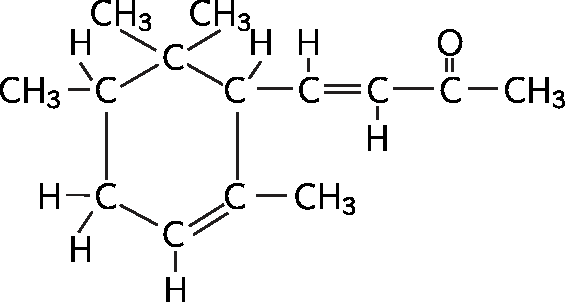
\includegraphics[width=0.4\textwidth]{Chapter1/α鸢尾酮香料的分子结构图}
    \caption{α鸢尾酮香料的分子结构图}
    \label{figure:α鸢尾酮香料的分子结构图}
\end{wrapfigure}
图\ref{figure:α鸢尾酮香料的分子结构图}是α鸢尾酮香料的分子结构图。

我们怎么\uwave{知道}存在着原子呢?可以用上面提到过的一种技巧:我们\uwave{假设}存在着原子,而一个又一个的结果与我们的预言相符合,如果事物真\uwave{是}由原子组成的话,它们就应当如此。此外,也多少有点更为直接的证据,下面就是一个很好的例子。由于原子是如此之小,你用光学显微镜观察不到它,事实上,即使用\uwave{电子}显微镜也不行。(用光学显微镜,你们只能看到大得多的的东西。)要是原子一直在运动,比如水中的原子,那么如果我们把某种较大的球放到水中去,这个比原子大得多的球就会晃来晃去——就像玩球时,一个很大的球被许多人打来打去一样。人们向各个方向推球,结果球在场地上作不规则运动。同样,“大球”也将运动,因为它在各个方面受到的碰撞不等,在各个时刻受到的碰撞也不等。因此,如果我们用很好的显微镜观察水中很小的粒子(胶粒),就能看到微粒在不停地跳动,这是原子碰撞的结果。这种运动称为\uwave{布朗运动}。

我们在晶体结构上也可看到进一步的证据。在许多情况下,由X射线分析推断出的结构在空间“形状”上与自然界中的晶体实际上显示出来的形状相符合。实际晶体的各个“面”之间的夹角,与从晶体是由多“层”原子构成的假设推断出来的角度之差在秒以下。

\uwave{一切都由原子构成}。这就是关键性的假设。例如,在整个生物学中最重要的假设是:\uwave{动物所作的每件事都是原子做的}。 换句话说:\uwave{没有一件生物做的事情不能从这些生物是用} \uwave{服从物理定律的运动原子组成的这个观点来加以理解}。这在开始并没有认识到:提出这种假设需要做一些实验与推理,但现在它已被接受了,它是在生物学领域内产生新观念的最有用的理论。

如果一块由一个挨一个的原子组成的钢或盐可以具有这种有趣的性质:如果水——它只不过是些小滴,地球上到处都有——可以形成波浪和泡沫,那这些波浪冲向水泥堤岸时会产生冲击声和奇妙的浪花;如果一流溪水永远只能是一堆原子,那么还会有什么呢?假设我们不是把原子排成确定的形式,再三重复,不断反复,或者甚至形成向紫罗兰香气那样复杂的东西,那么事情会变得更加不可思议吗?——那个在你面前走来走去与你攀谈的东西可能是一大群排列的非常复杂的原子吗?这个东西的彻底复杂性可能动摇你对它产生一些什么想象吗?当我们说,我们是一堆原子,这并不意味着我们\uwave{只是}一堆原子,当你站在镜子前,你就能在镜子里看到,一堆并非简单地一个一个重复排列的原子所组成的东西将会具有如何丰富和生动的内容!


\chapter{基本物理}

\section{引言}

在本章中,我们将考察有关物理学的最基本概念——即我们在目前所知道的事物的本性。这里将不去涉及我们如何知道所有这些观念是正确的那个认识过程,你们在适当的时候会学习到这些具体的细节。

我们在科学上所关心的事物,具有无数形式和许多属性。举例来说,假如我们站在岸边眺望大海,将会看到:这里有海水、拍击的浪花、飞溅的泡沫以及汹涌的波浪,还有太阳、光线、蔚蓝的天空、白云以及空气的流动——风;在海边有沙粒,不同色纹和硬度的岩石;在海里浮游着生物,此生彼灭;最后,还有我们这些站在海岸边的观察者;甚至还有幸福和怀念。在自然界的其他场合,难道不也同样出现如此纷繁复杂的事物和影响吗?无论在哪里,到处都是这样错综复杂和变化无穷。好奇心驱使我们提出问题,把事物联系起来,而将它们的种种表现理解为:或许是由较少量的基本事物和相互作用以无穷多的方式组合后所产生的结果。

例如,沙粒和岩石是两回事吗?就是说,沙粒只不过是大量的细小石块吗?月亮是不是一块巨大的岩石呢?如果我们了解岩石,是否就能了解沙粒和月亮呢?风是否与海洋中的水流相似,就是一种空气的流动?不同的运动有什么共同特征?不同的声音有什么相似之处?究竟有多少种颜色?等等,等等。我们就是试图这样地逐步分析所有的事情,把那些乍看起来似乎不相同的东西联系起来,希望有可能\uwave{减少不同类}事物的数目,从而能更好的理解它们。

几个世纪以前,人们想出了一种部分解答这类问题的方法,那就是:\uwave{观察},\uwave{推理}和\uwave{实验};这些内容构成了通常所说的\uwave{科学方法}。在这里,我们将只限于对那些有时称之为基本物理中的基本观点,或者由于应用科学方法而形成的基本概念作一描述。

现在我们要问:所谓“理解”某种事情指的是什么意思?可以作一想象:组成这个“世界”的运动物体的复杂排列似乎有点像是天神们所下的一盘伟大的象棋(这里指的是国际象棋——译者注),我们则是这盘棋的观众。我们不知道弈棋的规则,所有能做的事情就是\uwave{观看}这场棋赛。当然,假如我们观看了足够长的时间,总归能看出几条规则来,这些弈棋规则就是我们所说的基本物理。但是,即使我们知道了每条规则,仍然有可能不理解为什么下棋时要走某一步棋,这仅仅是因为情况太复杂了,而我们的智力却是有限的。如果你们会下棋,就一定知道,学会所有的规则是容易的,但是,要选择最好的一着棋,或者要弄懂别人为什么走这一着棋,往往就很困难了。在自然界里,也正是如此,而且只有更难一些。但是,至少我们能发现所有的规则。实际上我们今天还没找到一切规则(时而会出现一些像弈棋中“以车护王”那样的情况,使我们仍然感到无法理解)。除此之外,我们确实能用已知规则来解释的事情也是非常有限的,因为几乎所有的情况都是极其复杂的,我们不能领会这盘棋中应用这些规则的走法,更无法预言下一步将要怎样。所以,我们必须使自己只限于弈棋规则这个比较基本的问题。如果我们知道了规则,就认为“理解”了世界。

如果我们不能很好的分析这盘象棋游戏,那么又怎样来辨别我们“猜测”出的规则实际上是否正确呢?大致地讲,可以有三种办法。第一,可能有这种情况:大自然安排的,或者说我们将大自然安排的十分简单,只有少数几个组成部分,从而使我们能够正确地预测将要发生的事。在这种情况下,就能检验我们的规则是怎样起作用的。(在棋盘角落里可能只有少数几个棋子在移动,所以我们能够正确地解决。)

第二种检验规则的好办法是,利用那些由已知规则推导出来的一些较一般性的法则来检验已知规则本身。比如,象在棋盘中移动的规则是只许走对角线,因而我们可以推断,无论象走了多少步,它总是出现在红方块里。这样,即使不能领会细节,我们也总能检验有关象的走法的概念,只要弄清楚它是否一直在红方块里。当然,在相当长的时间里,它都将如此,直到突然发现它出现在黑方块里。(显然,这时发生的情况是这个象被俘获了,另一个卒走过来成为皇后,红方块里的象就变成黑方块里的象。)这也就是物理学中出现的情况,即使我们不能领会其中的细节,但是在相当长的时期内我们仍有在各方面都很好地起作用的规则;但是在某个时候,我们又会发现新的规则。从基本物理的观点来看,最有趣的现象当然是在那些\uwave{新的}场合——那些已知规则行不通的场合中所出现的现象,而不是在原有规则行得通的地方发生的现象!这是我们发现新规则的一条途径。

第三个鉴别我们的观念是否正确的方法比较粗糙,但或许是所有方法中最为有效的。这就是用粗略的近似方法来加以辨别。我们可能说不出为什么阿莱克因(Alekhine)\footnote{世界著名弈棋手,系国际象棋大师。曾多次获得国际象棋世界冠军。——译者注}要走这步棋,但是我们或许能大致认为它或多或少地在调集一些棋子到王的周围来保护它。因为这是在这种情况下明摆着的事。同样,根据我们对这盘棋的理解,即使不能看出每一步棋的作用,也常常能对自然界多少有所理解。

人们首先把自然界中的现象大致分为几类,如热、电、力学、磁、物性、化学、光或光学、X射线、核物理、引力、介子等等现象。然而,这样做的目的,是将\uwave{整个自然界}看作是一系列现象的许多不同侧面。这就是今天基础理论物理面临的问题:\uwave{发现隐匿在实验后的定律};\uwave{把各类现象综合起来}。在历史上,人们总能做到这一点,但随着时间的推移,新的事实发现了;我们曾经将现象综合得很好,突然,发现了 X 射线,随后我们又融合了更多事实,但是又发现了介子。因此,在弈棋的任何一个阶段,看起来总是相当凌乱。大量事实被归并了,但总还有许多线索向一切方向延伸出去。这就是今天的状况,也就是我们将试图去描绘的现状。

历史上出现过的若干进行综合的情况有如下几个。首先,是\uwave{热}与\uwave{力学}的综合,当原子运动时,运动得越是剧烈,系统所包含的热量就越多,这样,\uwave{热和所有的温度效应}可以用力学定律来说明。另一个巨大的综合,是发现了电、磁、光之间的联系,从而知道它们是同一件事物的不同方面,即今天我们称为\uwave{电磁场}的那个东西的不同表现。还有一个综合,是把化学现象、各种物质的各种性质以及原子的行为统一起来,这就是\uwave{量子化学}的内容。

显然,现在的问题是:能不能继续把所有的事情都综合起来,并且仅仅发现这整个世界体现了\uwave{一件}事情的种种不同方面?无人知道答案如何,我们所知道的只是:这样做下去时,我们发现可以综合一些事实,随后又发觉出现了一些不能综合的事实。我们继续尝试这种拼图游戏。至于是否只有有限数量的棋子,甚至这场拼图游戏是否有底,当然不知道。除非有那么一天终于把拼图拼成了,否则我们就永远不会知道事情的究竟。在这里我们要做的是,看看那种综合已经到了什么程度,在借助于最少的一组原理来理解基本现象方面,现状又是如何。简言之,\uwave{事物是用什么构成的}?\uwave{总共存在多少基本元素}?

\section{1920年以前的物理学}

一开始就从现在的观点讲起是有点困难的,所以让我们先来看一下在1920年左右人们是怎样看待世界的,然后再从这幅图像中挑出几件事情来。在1920年以前,我们的世界图像大致是这样的:宇宙活动的“舞台”是欧几里德所描绘的三维几何\uwave{空间},一切事物在称为\uwave{时间}的某一种媒质里变化,舞台上的基本元素是\uwave{粒子},例如原子,它们具有某些\uwave{特性},首先一个特性是惯性:如果一个粒子正在运动,那么它将沿着同一个方向继续运动下去,除非有\uwave{力}作用其上。此外,第二个基本元素就是\uwave{力},当时认为共有两类力。第一类力是一种极其复杂细致的相互作用,它们以复杂的方式将各种各样的原子约束在不同的组合之中,它们确定当温度升高时,食盐是溶解的更快还是更慢些;另一类已知的力是一种长程的相互作用,它是与距离平方成反比的变化平缓的作用力,称为万有引力。这条定律已为我们所知,它是很简单的。当然,\uwave{为什么}物体的运动一经开始就能保持下去,或者说\uwave{为什么}存在一条万有引力定律,我们则不清楚。

对自然的描述正是我们在这里要关心的。从这个观点出发,气体以及实际上\uwave{所有}的物质都是无数运动着的原子。这样,我们站在海边所听见到的许多东西马上可以联系起来了。首先是压力,它是来自原子与墙或者某个东西的碰撞;如果原子的运动平均而言都是沿着一个方向,这种原子的漂移运动就是风;而无规则的内部运动就是热。某个地方有过多的原子集结在一起时,就形成了过剩密度的波,当波前进时,把成堆的原子推向更远的地方,等等。这种过剩密度的波就是声波。能够理解这么多事情的确是惊人的成就。在前一章里,我们已经说明过一些这样的事情。

粒子有哪些种类?在当时认为有 92 种:那时已经发现有 92 种不同的原子,各按其化学性质而被赋予不同的名称。

其次的问题是“短程力”是什么?为什么碳吸引一个(有时两个)而不是三个氧?原子间的相互作用的机制是什么?是万有引力吗?答案是否定的。万有引力实在是太弱了。于是让我们来设想一种类似于力与距离平方成反比的力,不过在强度上远远超过前者,此外还有一个差别:在重力作用下,每个物体彼此吸引,但现在我们设想有\uwave{两}类“物体”,而这种新的力(当然就是所谓电力)具有同号相斥而异号相吸的特性。具有这样强的作用的“物体”就称为\uwave{电荷}。

那么,我们会得到什么结果呢?假定我们有两个异号电荷,一正一负,并且彼此十分靠近。现在,在若干距离之外,还有另一个电荷。它会感到吸引吗?\uwave{实际上}它几乎\uwave{不}会感到什么作用,因为如果前两个电荷的大小相等,来自一个电荷的吸引被来自另一个电荷的排斥所抵消。所以,在任何可观的距离外只有很小的一点作用力。另一方面,如果我们使第三个电荷\uwave{非常靠近}前两个时,就会发生吸引作用。因为同号电荷的斥力与异号电荷的引力倾向于使异号电荷靠近而使同号电荷远离。这样,排斥作用就将小于吸引作用。这就是为什么由正、负电荷组成的原子相互离开较远时只能感受到很小一点作用力(重力除外),而当它们彼此靠近时,就能够互相“看到内部”而重新安排其电荷,结果产生了极强的相互作用。原子间作用力的最终基础是电的作用。由于这种力是如此巨大,以至所有正的与负的电荷通常都以尽可能紧密的方式结合在一起。所有的事物,甚至我们自己,都由极精细的和彼此强烈作用着的正、负微粒所组成,所有正的微粒与所有负的微粒正好抵消。有时,碰巧我们“擦”去了一些负电荷或正电荷(通常擦去负电荷较为容易),在这种情况下将会发现电力\uwave{不再平衡},于是就能看到电的吸引作用。

为了对电力作用究竟比引力作用大多少有个概念,我们举出大小为 1 毫米,相距为 30 米的两粒沙子为例。假如它们之间的作用力没有抵消,每个电荷都吸引所有其他电荷而不考虑同号电荷间的斥力,因此不会抵消,那么,两颗沙粒之间的作用力会有多大呢?两者间将会产生三百万吨的力!你瞧,只要正电荷或负电荷的数目有一点点\uwave{极小}的过剩或欠缺,就足以产生可观的电效应。当然,这就是你们为什么不能看出带电体与非带电体之间的差别的原因——所牵涉的粒子数目少得无论在物体的重量上或者形状上都很难造成什么差别。

有了这样的图像,对原子就比较容易理解了。人们认为原子的中心是一个带正电的质量甚大的“原子核”,核周围围绕着一定数量的很轻而且带有负电的“电子”。让我们稍稍超前一点提一下:在原子核里也发现了两类粒子——质子和中子,它们的重量几乎相同,并且十分重。质子带正电,中子则呈中性。如果我们有一个原子,其核内有六个质子,从而四周环绕六个电子(在通常的物质世界中负粒子都是电子,与组成原子核的质子和中子相比,它们是很轻的)。在元素周期表上这个原子的序数是 6,名称是碳。原子序数为 8 的物质叫做氧,等等。因为化学性质取决于核外的电子,实际上它只取决于核外有\uwave{多少}电子。所以,一种物质的\uwave{化学}性质只由电子的数目所决定。(化学家的全部元素的名称实际上可以用 1,2,3,4,5 等等编号来称呼。)我们可以说“元素六”,表示六个电子,以代替“碳”这个名称。当然,在先前发现元素时,人们并不知道它们可以用这种方式来编号。此外,这又会使事情复杂化,因此,宁可对这些元素定一个名称和符号,这比用编号来称呼元素来得更好。

关于电的作用,人们还发现了更多事情。对电相互作用的自然解释是,两个物体简单地互相吸引:正的吸引负的。然而后来发现用这种观点来描写电的相互作用并不妥当。更合适的描述这种情况的观点是:在某种意义上,正电荷的存在使空间的“状况”发生畸变,或者说在空间造成了一种“状况”。于是当我们将负电荷放到这个空间里后,它就会感受到一个作用力。这种产生力的潜在可能性就叫做\uwave{电场}。当把一个电子放入电场时,我们就说它受到“拉拽”。于是我们就有两条规则:(1)电荷产生电场;(2)电荷在电场中会受到力的作用而运动。如果我们讨论下述现象的话,建立这条规则的理由就清楚了:假如我们使某物体比方说梳子带电,然后把一张带电的纸片放在一定距离之外,当我们来回移动梳子时,纸片就会有反应,并且总是指向梳子。如果我们使梳子晃动的快些,就会发现纸片的运动有一点滞后,即作用有所延迟。(起先,当我们相当慢地晃动梳子时,我们发现一种错综复杂的现象,这就是磁。磁的影响与作相对运动的电荷有关,所以磁力和电的作用力实际上可以归之于一个场,这象同一件事的两个不同的方面。变化的电场不能离开磁而存在!)假如我们把纸片移得更远,滞后就更大。这时能观察到一件有趣的事:虽然两个带电体之间的作用力应当与距离的\uwave{平方}成反比,但是我们发现当摇动一个电荷时,电作用的影响范围要比起初所猜想的\uwave{大得多}。这就是说,作用的减弱要比反平方的规则来的慢。

这里有一个类比:如果我们在水池里,而在近处漂浮着一个软木塞,我们可以用另一个软木塞划水来“直接”移动那个木塞。如果现在你只注意两个\uwave{软木塞},你能看到的将是一个立即响应另一个的运动——在软木塞之间存在着某种“相互作用”。当然,我们实际上所做的只是搅动了\uwave{水};然后水又去扰动另一个木塞。于是,我们就能提出一条“定律”:如果稍微划一下水,那么水中附近的物体就会移动。当然,假若第二个软木塞离得较远,它将几乎不动,因为我们只是\uwave{局部地}搅动水。另一方面,假如我们晃动木塞,就会产生一个新的现象,这部分水推动了那部分水,等等,于是\uwave{波}就传播开去。这样,由于晃动,就有一种波及\uwave{十分远}的影响和一种振荡的影响,这是无法用直接相互作用来理解的。所以那种直接作用的概念必须用水的存在来代替,或者,对于电的情形,用我们所谓的电磁场来代替。

电磁场能传送各种波。其中的一些就是\uwave{光}波,另一些波用在\uwave{无线电广播里}。但它们总的名称是\uwave{电磁波}。这些振荡的波可以有各种\uwave{频率},一种波和另一种波之间的唯一的真正差别只是\uwave{振荡的频率}。假如我们越来越快地来回晃动电荷,并且注视着所产生的效应时,我们将得到一系列不同的效应,只要用一个数,即每秒钟振荡的次数,就能把这些效应统一起来。通常在我们住房墙上电路里流动电流所产生的扰动约为 100 周/秒。如果我们把频率提高到每秒 500 千周或 1000 千周(1 千周 = 1000 周),我们就“在空气中”了\footnote{原文为“On the air”,直译为“在空气中”,亦作电台“正在广播”解。作者在这里用的是双关语,故有下文的“广播与空气毫无关系”。——译者注}因为这正是无线电广播所用的频率范围(当然,广播与\uwave{空气}毫无关系!没有任何空气也能进行广播)。假如再提高频率,那么就进入调频广播和电视所用的波段。再上去,我们使用一种极短的波,比如雷达所用的波。频率再增高,我们就无需用仪器来“看”这种波了,而用眼睛就能看到它。在频率范围为每秒$ 5\times10^{14} $  到$ 5\times10^{15}  $ 周的时候,只要有可能使带电的梳子晃动的这样快,我们的眼睛就能见到带电梳子的振动像红光、蓝光或紫光,视振动的频率而定。低于上述频率范围的称为红外,高于此范围的称紫外。从物理学家的观点来看,我们能看见某种频率范围的波这个事实并不使这一部分电磁波谱比其他部分有什么更令人注意的地方,但是从人类的观点来看,这当然\uwave{是}更有趣的。如果我们把频率提得更高,于是就得到 X 射线,X 射线不是别的,只是频率极高的光而已。如果再提高频率,就得到 γ 射线。X 射线与 γ 射线这两个名称在使用时几乎是同义的,通常将原子核发出的电磁射线称为 γ 射线,而从原子中发出的这种高能的电磁射线就成为 X 射线,但是不论它们的起源如何,当频率相同时,它们在物理上是无法区别的。如果我们能进到更高的频率,比如说每秒$10^{24}$周,我们发现可以人工制造这样的波,例如用加里福尼亚工学院的同步加速器。我们还可以在宇宙射线里发现频率出奇地高——具有甚至快1000倍的振荡——的电磁波,而这些波目前还不能由我们来控制。

\begin{table}[H]
    \centering
    \label{tab:电磁波谱}
    \caption{电磁波谱}
    \medskip 
    \begin{tabular}{@{}lll@{}}
        \toprule
        频率(周/秒)                     & 名称         & 大略行为 \\ \midrule
        $10^{2}$                    & 电扰动        & 场    \\
        $5\times10^{5}\sim10^{6}$   & 无线电广播      & 波    \\
        $10^{8}$                    & FM-TV      & 波    \\
        $10^{10}$                   & 雷达         & 波    \\
        $5\times10^{14}\sim10^{15}$ & 光          & 波    \\
        $10^{18}$                   & X射线        & 粒子   \\
        $10^{21}$                   & γ射线(核)     & 粒子   \\
        $10^{24}$                   & γ射线(“人造”)  & 粒子   \\
        $10^{27}$                   & γ射线(宇宙射线中) & 粒子  \\ \bottomrule
    \end{tabular}
\end{table}


\section{量子物理学}

说明了电磁场概念和电磁场能传送波后,我们很快就认识到,这些波的行为实际上十分奇怪,看起来完全不像波。在频率较高时,它们的行为更像\uwave{粒子}!正是在1920年后发展起来的量子力学解释了这种奇怪的行为。在1920年之前,爱因斯坦已改变了把空间看作是三维空间、把时间看成是单独存在的这种图像。他首先把它们组合在一起,并称之为空-时,然后又进一步用弯曲的空-时来描绘万有引力。这样,宇宙的“舞台”就变为空-时,而万有引力则大概是空-时的一种变态。以后,人们又发现有关原子运动的规则也是有问题的:在原子世界中,“惯性”与“力”的力学法则是不正确的——牛顿定律已不再成立。人们反而发现小尺度范围内事物的行为与大尺度范围内事物的行为没有任何相似之处。这给物理学造成困难——但又十分有趣。之所以困难,是由于事物在小尺度范围内的表现如此“反常”,我们对之没有直接的经验。在这里事物的表现完全不像我们所知道的任何事情,因而除了用解析的方式,用任何其他方法都不可能描写这种习性。这的确是困难的,需要做大量的想象。

量子力学中有许多看法。首先,一个粒子既有确定的位置也有确定的速度,这种概念已被抛弃,那是不正确的想法。表明经典物理是怎样不正确的一个例子是,在量子力学中有这样一条定则:不可能既知道某个粒子在什么地方,又知道它运动得多块。动量的不确定性与位置的不确定性是并协的,二者的乘积是常数。我们可以把这条定律写成$ \Delta x\,\Delta p\geq\hbar/2 $,在以后将会更详尽的解释它。这条定则解释了这样一个十分神秘的佯谬:即如果原子是由正负电荷所构成,那么为什么负电荷不是简单地位于正电荷的顶端(它们彼此是吸引的),从而彼此靠拢以至于完全抵消?\uwave{为什么原子如此庞大}?为什么原子核在中心,而其周围环绕着一些电子?起先曾认为原子核很大,但事实并非如此,它是\uwave{非常小}的。一个原子的直径约为$ 10^{-8} $厘米,一个原子核的直径约为$ 10^{-13} $厘米。如果我们有一个原子,为了看到原子核,就要把整个原子放大到一个大房间大样大。这时原子核才刚刚是一个可以用眼睛分辨出来的斑点,但是几乎原子所有的重量都集中在这个无比小的原子核上。是什么理由使电子没有直接落入原子核呢?正是上述的原理。如果电子在原子核里出现,我们就会精确地知道它们的位置,而测不准原理则要求它们具有很大的(不过是不确定的)动量,即很大的动能。电子具有这样大的能量就要脱离原子核,这些电子作出了让步:由于不确定性,它们为自己留下一个狭小的空间,于是以由这个定则所决定的最小的运动晃动着。(记得我们曾经说过,当晶体冷却到绝对零度时,原子并没有停止运动,它们仍然在晃动,为什么?如果它们停止运动,我们就能知道它们在什么地方,而且它们不运动,这就违反了测不准原理:我们不能既知道它们在哪里,又知道它们以什么速度运动。所以它们必须在那里不断地摆动!)

另一个由量子力学带来的在科学的观念和哲学方面最有趣的变化是,在任何情形下要想精确地预言会发生什么事都是不可能的。比如我们有可能使一个原子处于准备发光的状态,在原子发光时,可以利用探测光子的方法进行测量(这一点我们马上就要讲的),但是,我们无法预计它将在什么时候发光,或者在有几个原子的情况下,究竟哪一个原子将发光。你们可能说,这是由于某种我们还没有足够仔细观察过的内部“转轮”在起作用。然而,这里根本没有什么内部的转轮,按照我们今天的理解,大自然的表现是这样的:根本不可能精确地预言在一定的实验中究竟会发生什么事情。这是一件糟透了的事;事实上,哲学家曾声称:科学所必需的基本东西之一就是,每当你安排了同样的条件时,那么发生的必定是同一件事。但是,这完全不正确,它并不是科学的基本条件。事实上是所发生的并不是同一件事,我们所能得到的只是发生一些什么的统计平均。不过,科学并没有完全崩溃。顺便地说,哲学家们讲了一大套科学之绝对必需是什么,但就像人们所看到的那样,这些总是相当天真的,甚至还是错误的。例如,某个哲学家宣称对科学的成就来说十分重要的是,如果同一个实验先在某处,比如说在斯德哥尔摩做;然后在另一处,比如说在基多(南美厄瓜多尔首都——译者注)做,那么必定会出现同样的结果。这纯粹是一派胡言。对科学来说,这并不是必然的:它可能是一个经验事实,但不是必然的情况。比如有一个实验室在斯德哥尔摩观察天空,这时会看到北极光,如果在基多则看不到这种现象,这就是出现了不同的情况。“但是”,你会说:“这是一件与外部情况有关的事,如果你把自己关在斯德哥尔摩的一个房间里,拉下窗帘的话,那么会发生什么差别吗?”肯定会。假如我们在一个方向接头上挂一个摆,让它开始摆动,它就会差不多在一个平面里摆动,但也并不完全如此。在斯德哥尔摩,平面会缓慢地转动着,但是在基多就不会。在那里,窗帘也是垂下的。这件事的发生并没有引起科学的毁灭。科学的基本假设,它的基本哲学观念是什么呢?我们在第一章里讲到过:\uwave{实验是任何观念的正确性的唯一试金石}。假如结果是在基多所作的大多数实验与在斯德哥尔摩所作的实验效果一样,那么这“大多数实验”就可用来提出某种一般性的定律,至于对那些效果不同的实验,我们就将说:“这是由于斯德哥尔摩周围的环境不同所引起的”。我们将能想出一些办法来概括实验结果,而没有必要在事先就被告诫说,这些办法看起来象什么。假如有人告诉我们说,同样的实验总是产生同样的结果,这固然很好。但是当我们试了一下后,发现并非如此,因而结论的确就是并非如此。我们正是必须相信自己所看到的,然后才能借助于实际的经验来形成我们的一切其他观念。

现在让我们回到量子力学和基本物理上来。当然,我们在此刻还不能详细叙述量子力学的原理,因为它们是颇难理解的。我们将假定它们成立,然后叙述一下某些结果。其中一个是,我们通常视作为波的那些事物也具有粒子的习性,而粒子则具有波的习性。实际上,每一种事物的行为都是一样的,不存在波和粒子的区别。这样,量子力学就将场的概念以及场的波与粒子统一起来。的确,频率低时,现象的场的方面比较明显,或者说作为根据日常经验的近似描写时比较有用。但当频率增加时,现象的粒子方面对于我们通常用来作为测量用的仪器来说更为明显。实际上,虽然我们提到过许多频率,但目前还没有探测到任何直接涉及频率在每秒$10^{12}$周以上的现象,我们只是在假定了量子力学的波粒二象性概念是正确之后,根据有关规则从粒子的能量来推断出这些较高的频率的。

于是,我们对电磁相互作用有了新的见解。我们把一种新的粒子加入到电子、质子及中子的行列,这种新的粒子称为光子。新的电子质子相互作用的见解称为量子电动力学,它就是电磁理论,不过其中的一切在量子力学上都是正确的。这是光和物质,或电场与电荷之间的相互作用的基本理论,就物理学来说它是我们最伟大的成就。比如,从量子电动力学可以得出所有已知的电学、力学和化学定律:弹子碰撞的定律,导线在磁场中运动的定律,一氧化碳的比热,霓虹灯的色彩,盐的密度,以及氢气与氧形成水的反应等,全部都是这一理论的推论。所有这些细节,如果简单到能使我们运用近似方法的话,都可以得出,这实际上当然不可能。不过,我们总能对发生的事多少有所理解。目前,在原子核外面还没有发现量子电动力学定律有什么例外,对于原子核我们不知道是否会有例外,因为对于核内的过程我们简直还不太清楚。

这样,在原则上,量子电动力学是一切化学以及生命的理论——如果生命最后归结为化学,因而也就归结为物理的话(因为化学本身已经归结为物理,涉及化学中的那部分物理早就知道了!)。不仅如此,量子电动力学这个伟大的理论还预言了许多新的事实。首先,它说明了甚高能光子、γ 射线等等的性质。它还预言了另一个十分出乎意外的事:除电子外,还应当有同样质量、但带有正电荷的称为正电子的粒子,并且这两种粒子碰在一起时,会彼此湮没而放出光或 γ 射线(其实,光与 γ 射线完全是一回事,只是频率不同而已)。这件事情的推广——即对每个粒子总有一个反粒子——现在知道是正确的。电子的反粒子有另一个名称,即正电子。但其他大多数反粒子,就称反某某子,如反质子、反中子。在量子电动力学中,提出了两个基本数据——电子质量与电荷,所有世界上其他的数被认为可以从这两个数据推导出来。实际上,这不完全正确,因为化学还有一整套数据,它告诉我们原子核是多重,这就把我们引导到下一部分内容中去了。


\section{原子核与粒子}

原子核是由什么组成的,这些东西又是怎样结合在一起的?人们发现,原子核是靠巨大的作用力结合在一起的,当这种力释放时,其释放出来的能量比化学能大得多。前者与后者之比就好像原子弹爆炸与 TNT 炸药的爆炸相比一样。当然,这是因为原子弹爆炸时与原子核里的变化有关,而 TNT 的爆炸则与原子外层的电子变化有关。问题是,究竟是什么力使原子核中的质子与中子结合在一起呢?汤川秀树提出,就好像电相互作用可以与一种粒子——光子联系起来一样,中子与质子之间的作用力也有某种场,当这个场晃动时,就好像一个粒子一样。所以除去中子与质子外,在世界上应当有一些别的粒子,而汤川能从已知的核力特征推导出这些粒子的性质。比如,他预言它们应当有二、三百个电子那样大的质量。你瞧!在宇宙间竟然真的发现了这样质量的粒子!但是,后来发现这并不正是预言的粒子,它被称为$\mu$介子。

然而,没有过多少时候,在 1947 年或 1948 年就发现了另一个粒子—— $\pi$介子,它满足汤川的判据。这样,除去质子与中子外,为了得到核力,我们还必须加上$\pi$介子。你可能会说,“太好了!借助这个理论就可以象汤川所希望的那样建立起利用$\pi$介子的量子核动力学。然后看它是否成立,如果成立的话,那么每件事都可得到解释了。”不幸的是,包含在这个理论中的计算是如此困难,以至于一直到今天,已将近 20 年了,从来还没有一个人能够从这个理论中得出什么结果来,或者能够用实验去验证一下。

所以我们被这个理论难住了。我们不知道它究竟是正确的还是错误的,但却知道它有点小小的错误,或者至少是不完全的。正当我们在理论上徘徊并且试图用这个理论计算出结果来时,实验物理学家发现了一些事情。比如,他们早已发现了$\mu$介子,而我们却还不知道把它归到哪里去。而且,在宇宙射线里,还发现了大量的其他“额外”粒子。今天,我们已大约有近 30 种粒子,理解所有这些粒子的相互关系是非常困难的——大自然要它们来干什么?这一个粒子与另一个粒子之间的联系是什么?我们今天并没有把这些不同的粒子理解为同一件事情的不同方面。我们有这么多相互无关的粒子,这事件本身就表明了没有一个能够说明这么多相互无关的信息的良好理论。由于量子电动力学的伟大成功,我们具备了一定的核物理的知识,它是一种粗糙的、半经验、半理论的知识。假设一种质子与中子间的力的类型,然后看看会发生什么事情,但是并不确实知道力的来源。除此以外,我们很少取得进展。在化学上,人们曾搜集大量的化学元素,以后突然在元素之间出现一种没有预期到的关系,它就体现在门捷列夫元素周期表中。比如,钠和钾的化学性质几乎是相同的,它们就在周期表的同一行里。对于新粒子而言,我们一直在探索者这种门捷列夫式的表。有一张这样的新粒子表,是由美国的盖尔曼与日本的西岛各自独立作出的。他们分类的基础是一个新的数。类似于电子的电荷,这种新的数叫做“奇异数”$S$,对每个粒子都指定了这样一个数,它像电荷一样是守恒的,即在核力的反映中保持不变。

图2.1列出了所有的粒子。眼下我们对之还无法讨论得很多。但是这张图片至少向你们表明,我们不知道的东西有多少。每个粒子下写着它的质量,其单位是 MeV(兆电子伏)。1MeV 等于$ 1.783\times10^{-27} $克。选取这种单位的理由是出自历史的原因,我们现在不去说它。质量大的粒子在表中放在较高的位置;可以看到中子与质子的质量是差不多的,在垂直的栏内的粒子都有同样的电荷,所有的中性粒子都放在同一栏内,所有带正电的粒子在这一栏的右边,所有带负电的粒子则在左边。

\begin{figure}
    \centering
    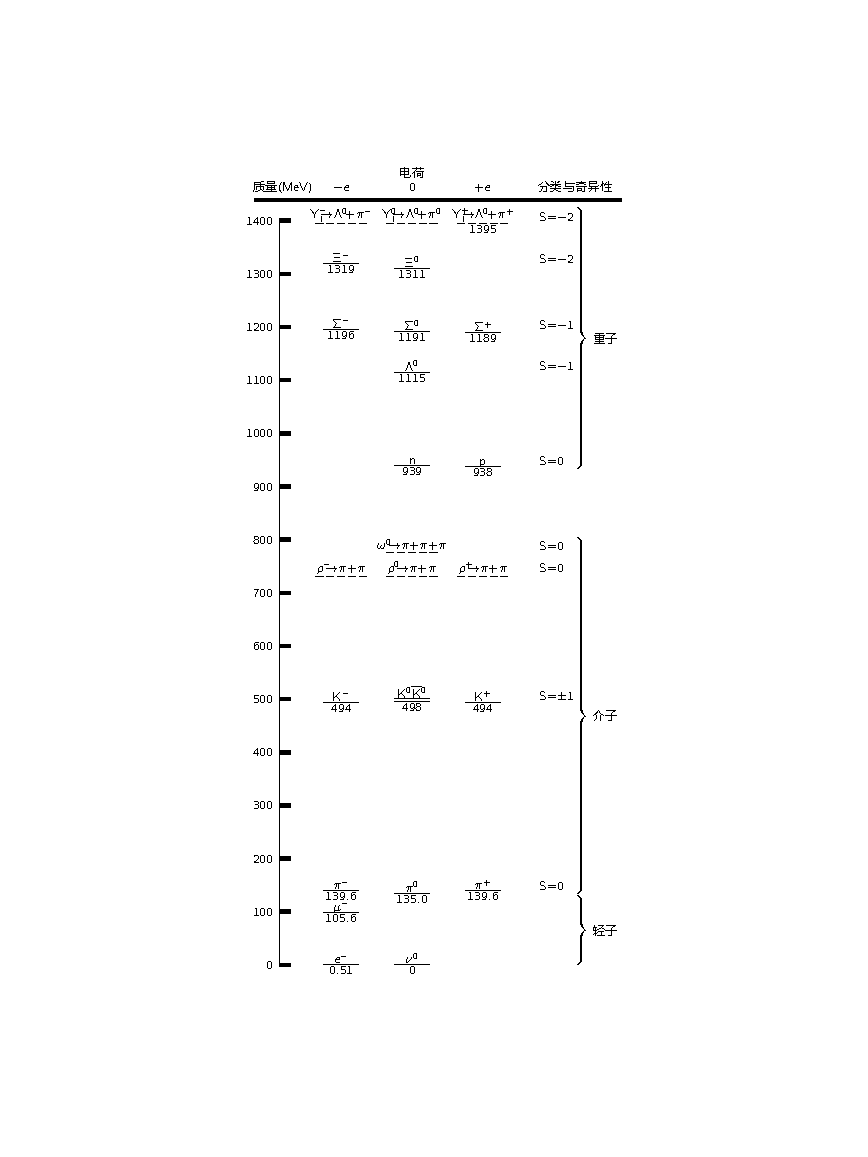
\includegraphics[width=0.65\textwidth]{Chapter2/基本粒子}
    \caption{基本粒子}
    \label{figure:基本粒子}
\end{figure}

图2.1中实线标出的是粒子,虚线标明的是“共振态”。图中略去了几个粒子,包括重要的零质量、零电荷的粒子,即光子与引力子;它们并不属于重子-介子-轻子分类图。此外,还有某些较新的共振态($K^*$,$\phi$,$\eta$)也不包括在这里。介子的反粒子也列在表格内,但轻子与重子的反粒子就需要另列一张表了,它看起来正好是前面那表格对零电荷栏的反演。虽然除去电子、中微子、光子、引力子和质子外,所有的粒子都是不稳定的,但是在这里只列出了共振态的衰变产物。奇异数并不适用于轻子,因为它们与核之间并没有强作用。

所有与中子、质子放在一起的粒子统称为\uwave{重子}。共存在着以下几种:$\lambda$介子,质量为 1154MeV 。另外三个:($ +\Sigma $)介子,($ -\Sigma $)介子,$ \Sigma $介子,质量是相近的。这里还有成群或者说成\uwave{多重态}的粒子,带有差不多相同的质量,相差不到百分之一或二。在多重态内的每个粒子都有同样的奇异数。第一个多重态是质子-中子二重态,以后是单重态($\lambda$介子),再以后是 $ \Sigma $三重态,最后是$ \Xi $二重态。最近,在1961年,又发现少数几个粒子,但它们都是粒子吗?它们的寿命是如此短暂,当刚形成时,几乎就立刻蜕变了,所以我们不知道,它们究竟应被认为是新的粒子,还是在它们蜕变成$\lambda$介子及$\pi$介子时,后二者之间某种确定能量的“共振”作用呢?

除去重子外,其它包括在核内相互作用中的粒子称为介子。首先是$\pi$介子,有三种形态:正、负及中性;它们组成了另一多重态。我们还发现一些新的称为K介子的粒子,它们作为$ K^{+} $及$ { K }^{ 0 } $而出现。其次,每个粒子都有反粒子,除非一个粒子是它自己的反粒子。例如$\pi^{-} $和$\pi^{+} $是一对反粒子,但是$\pi^0 $是它自己的反粒子;$K^- $及$ K^+ $是反粒子对,$ { K }^{ 0 } $及$ \bar {{ K }^{ 0 } }  $也是反粒子对。附带说一下,在 1961 年我们又发现了一些介子或可能的介子。它们几乎即刻就蜕变了,有一个称为$\omega$的东西带有 780MeV 的质量,分解为三个 $\pi$ 介子,有一个还不怎么确定的东西分解为两个$\pi$介子。那些被称为介子与重子的粒子与介子的反粒子放在同一张表格里,但重子的反粒子必须放到另一张通过零电荷栏“反射”而来的表格里去。

门捷列夫周期表示是完美的,除去有一些稀土元素挂在外面。同样,这里也有一些粒子挂在表外,它们在核内的相互作用不强,跟核相互作用根本无关,跟核之间也没有强相互作用。(我们所指的是那种强的核能相互作用。)它们被称为轻子,主要有如下几种:电子,其质量很小,只有 0.510MeV;然后是$\mu$介子,质量约为电子的 206 倍。根据所有的实验,我们今天所能说的是,电子与$\mu$介子之间的差别仅仅是质量不同而已,除了$\mu$介子比电子重外,其他二者都完全一样。为什么一个比另一个重?$\mu$介子有什么用?我们不知道;此外,有一种轻子是中性的,叫做中微子,具有零质量,事实上,现在知道有两类中微子,一类与电子有关,另一类与$\mu$介子有关。

最后,还有两种与核内其他粒子间没有强作用的粒子:一个是光子,另一个(或许)是具有零质量的引力子——假如引力场也有量子力学的类比的话(引力的量子化理论还没有建立)。

什么是“零质量”?这里所标明的质量是粒子\uwave{在静止时}的质量。事实上,一个粒子具有零质量在某种程度上就意味着它不可能\uwave{静止}。光子永远不会静止的,它一直以每秒 186,000 英里(300,000 公里)的速度运动。当我们在适当的时候学习了相对论的内容后,对于质量就会理解得更多一些。

这样,我们就面对着一大群粒子,它们看来都是物质的基本组成部分。幸运的是,这些粒子彼此之间的相互作用并不\uwave{全}都是不同的。事实上,粒子之间的相互作用看来可以分为四类,按强度降低的顺序排列时,它们就是:核力、电相互作用、$\beta$衰变作用以及引力。光子与所有带电粒子会发生耦合,作用的强度用某个数(1/137)来量度。这种耦合的详细定律已经知道,那就是量子电动力学。引力和所有的能量发生耦合,但它的耦合是非常弱的,远远小于电的作用,这条定律也已经知道了。然后,还存在着所谓的弱衰变——$\beta$衰变,它使中子蜕变为质子、电子及中微子,其过程是比较缓慢的,这种作用的定律只是部分地知道。还有所谓的强相互作用,介子-重子相互作用,其强度为1,它的规律完全不知道,虽然已经知道几条法则,譬如重子的数目在任何反应中都不改变。

这些就是当代物理学惊人的状况。总结一下,我们可以这样说,在核外,看来一切都知道了;在核内,量子力学是正确的,还没有发现量子力学原理失效的情况。可以说:容纳我们所有知识的舞台是相对论空-时;也许引力也包括在空-时之中。我们不知道,宇宙是怎样开始的,我们从来没有做过实验来精确地检查在某个微小距离下的空-时观念,所以只知道在哪个距离以上我们的空-时观念行得通。我们还应当补充说:这个伟大的象棋赛的规则就是量子力学的原理,到现在为止我们可以说,这些原则应用于新的粒子时,与应用于过去已经发现的粒子一样成功。核力的起源将我们引向新的粒子,但是遗憾的是,出现的粒子实在太多,以致使我们感到迷惑不解,虽然我们已经知道在它们之间存在着一些非常出人意表的关系,但对它们的相互关系缺乏完整的理解。看来我们正摸索着前进,逐渐趋于对亚原子粒子世界的理解。但是,我们实在不清楚,在这种摸索中我们还必须走多远。

\begin{table}[H]
    \centering
    \label{tab:基本相互作用}
    \caption{基本相互作用}
    \medskip 
    \begin{tabular}{@{}lll@{}}
        \toprule
        耦合关系      & 强度             & 定律         \\ \midrule
        光子对带电粒子   & $\sim10^{-2}$  & 已知         \\
        引力对所有其他能量 & $\sim10^{-40}$ & 已知         \\
        弱衰变       & $\sim10^{-5}$  & 部分已知       \\
        介子对重子     & $\sim1$        & 不知(部分法则已知) \\ \bottomrule
    \end{tabular}
\end{table}

\chapter{物理学与其他科学的关系}

\section{引言}

物理学是最基本的、包罗万象的一门学科,它对整个科学的发展有深远的影响。事实上,物理学是与过去所谓的“自然哲学”相当的现代名称,现代科学大多数就是从自然哲学中产生的。许多领域内的学生都发现自己正在学习物理学,这是因为它在所有的现象中起着基本的作用。在本章中我们试图说明其他科学中的基本问题是什么,当然,在这么一点篇幅内要真正地处理这些坝域中的复杂、精致而美妙的事情是不可能的。正因为篇幅较少,使我们不能讨论物理学与工程、工业、社会和战争之间的关系,甚至不能讨论数学与物理之间的最令人注目的关系。(按照我们的观点,从数学不是一门自然科学这个意义上来说,它不是一门科学,它的正确性不是用实验来检验的。)顺便提一下,我们必须从一开始就说清楚:如果一件事情不是科学,这并不一定不好。例如,爱好就不是科学。所以,如果说某件事不是科学,这并不意味着其中有什么错误的地方;这只是意味看它不是科学而已。

\section{化学}

也许受物理学影响最深的科学就是化学了。在历史上,早期的化学几乎完全讨论那些现在称为无机化学的内容,即讨论那些与生命体不发生联系的物质。人们曾经进行了大量的分析才发现许多元素的存在以及它们之间的关系——即它们是怎样组成在矿石、土壤里所发现的简单化合物的,等等。早期的化学对于物理学是很重要的。这两门科学间的相互影响非常大,因为原子的理论在很大程度上是由化学实验来证实的。化学的理论,即化学反应本身的理论,在很大程度上总结在门捷列夫周期表里,周期表体现了各种元素之间的许多奇特的联系,它汇总了有关的规则:哪一种物质可以与哪一种物质化合,怎样化合,等等,这些就组成了无机化学。原则上,所有这些规则最终可以从量子力学得到解释,所以理论化学实际就是物理。但是,必须强调的是,这种解释只是\uwave{原则上的}。我们已经讨论过了解下棋规则与擅长下棋之问的差别。也就是说,我们可能知道有关的规则,但是下得不很好。我们知道,精确地预言某个化学反应会出现什么情况是十分困难的;然而,理论化学的最深刻部分必定会归结到量子力学。

还有一门由物理学与化学共同发展起来的极其重要的分支,这就是把统计学的方法应用于力学定律起作用的场台,这被恰当地称之为\uwave{统计力学}。在任何化学状态中都要涉及大量的原子,我们已经看到原子总是以复杂而毫无规则的方式不停地晃动。假如我们能够分析每一次碰撞,并且跟踪每一个分子的运动细节的话,就能判断出将会发生一些什么,但是要记录所有这些分子就需要许许多多数据,这远远超过了任何计算机的容量,当然也一定超过人脑的容量,所以为了处理这样复杂的情况,重要的是要采取一种有效的方法。统计力学就是关于热现象或热力学的理论。作为一门科学,无机化学现在基本上已归结为所谓物理化学和量子化学;物理化学研究反应率和所发生的详细变化(分子间如何碰撞?哪一些分子先飞离?等等),而量子化学则帮助我们根据物理定律来理解所发生的事。

化学的另一个分支是\uwave{有机化学},它研究与生命体有关的物质。人们曾一度相信与生命有关的物质是如此神秘,因此不可能用我们的手从无机村料中制造出这种物质。这根本不对——它们与无机化学中制成的物质完全一样,只是包括了更复杂的原子排列。很明显,有机化学与提供有机物质的生物学之间有十分密切的关系,与工业也有密切的联系,而且许多物理化学和量子化学的定律不仅适用于无机化合物的情况,而且也适用于有机化合物。然而,育机化学的主要任务并不在于这些方面,而是在于分析、综合那些在生物系统以及在生命体中所形成的物质。这样就不知不觉地逐步引向了生物化学,然后是生物学本身,或分子生物学。


\section{生物学}

我们就这样进入了\uwave{生物学},它研究的是生命体。在生物学发展的早期,生物学家必须进行单纯的说明性工作——找出有\uwave{哪些}生物,所以他们要数数跳蚤足上的细毛之类的东西。当他们以很大的兴趣完成这种工作后,就进面考虑在生命体内部的\uwave{机制}问题。起先自然是从十分粗略的观点出发的,因为要知道更详细的情况是需要经过一番努力的。

在物理学与生物学的早期关系中有过一件很有趣的事,生物学曾经帮助物理学发现了\uwave{能量守恒定律},梅耶(Mayer)最先在关于生物吸收和放出的热量问题上证实了这条定律。

假如我们更仔细地观察动物的生物学过程,就会看到\uwave{许多}物理现象:血液的循环、心的跳动、血压等等。这里还有神经。如果我们踩在一块尖锐的岩石上,就会知道发生了什么事情,这个信息不知怎么地就从我们的脚底传递上来。有趣的是这个信息是怎样传递的。在研究神经时,生物学家得到了这样的结论:神经是非常精细的小管道,有十分薄而复杂的管壁;细胞通过这样的管壁吸进离子,所以在外面有正离子,而在里面则有负离子,就像一个电容器一样。这层薄膜还有一个有趣的性质:如果它在某个地方“放电”,即一些离子能够通过这个地方,那么该处的电压就减少,它会影响到邻近地方的离子,而这又会影响那里的薄膜,使它也让离子通过,接着这又要影响更远的薄膜,等等,于是在薄膜中就出现一列“穿透性变动”波,当神经末梢的一端由于碰到尖锐的岩石而受到“刺激”后,这种波就沿着神经传开来。它有点像一长列垂直放置的多米诺骨牌;如果末端的一个被推倒,邻近的一个也就被它带动,等等。当然,除非把多米诺牌再重新排好,不然,这时只有一个信息传递过去;类似地,在神经元里,也有排出离子的缓慢过程,使神经又处于准备接收下一个脉冲的状态。这就是为什么我们会知道正在做什么(或者至少知道我们在哪里)。当然我们可以用电子仪器测出这种与神经冲动有关的电的效应,因为这里\uwave{存在}着电的作用,十分明显,电效应的物理知识对理解这个现象很起作用。

相反的效应是从大脑中某个地方沿着神经发生一个信息。这时在神经的末梢会出现什么情况呢?神经在末梢处分成了细微的小纤维,这些小纤维与肌肉附近的一种称为端板的结构相连接。由于一些现在还不完全理解的原因,当脉冲信号抵达神经末梢后,射出一小团一小团称为乙酰胆碱的化学物质(每次约5到10个分子),它们影响了肌肉纤维而使其收缩——这一切多么简单!什么东西使肌肉会发生收缩呢?肌肉是由极多的彼此紧贴的纤维所组成的,它含有两种不同的物质:肌球蛋白和肌动球蛋白,但是由乙酰胆碱所引起的那种改变,分子大小的化学反应机制现在还不清楚。这样在肌肉中引起机械运动的基本过程也未为我们所知。

生物学的领域是如此广泛,有许多问题我们根本无法叙述,比如视觉是如何产生的(即光在眼睛里做什么),听觉是如何产生的,等等。(思维是如何进行的这一个问题将存后面心理学中讨论。)但是从生物学的观点来说,我们刚才所讨论的这些关于生物学的事情实在并不是基本的,并且不是生命的根源——即使我们理解了它们,仍然不能理解生命本身。举一个例子:研究神经的人感到他们的工作是很重要的,因为无论如何不存在没有神经的动物,但是没有神经仍然\uwave{可以}有\uwave{生命}。植物既无神经也无肌肉,但是它们照样活动着,照样生存着。所以我们对于生物学的基本问题必须更仔细地研究一下;如果我们这样做,就会发现所有的生命体中存在着许多共同的特征。最普遍的特征是它们都由\uwave{细胞}组成,每个细胞内都有起化学作用的复杂机制。例如,在植物细胞中就存在着接收光线而产生蔗糖的机构,植物在夜间消耗蔗糖以维持其生存。当动物摄取植物后蔗糖在动物体内就产生了一系列化学反应,这些反应与植物体内的光合作用(以及在夜间的相反作用)有很密切的关系。

在生命系统的细胞里有许多复杂的化学反应,在反直中一种化合物变成另一种化合物,然后再变成一种化合物。为了对生物化学研究中所付出的巨大的努力有某种印象,我们在图3-1中总结了到此刻为止所知道的在细胞中出现的反应,这些反应只是所有反应中的很小一部分,大约只占1%左右。

\begin{figure}
    \centering
    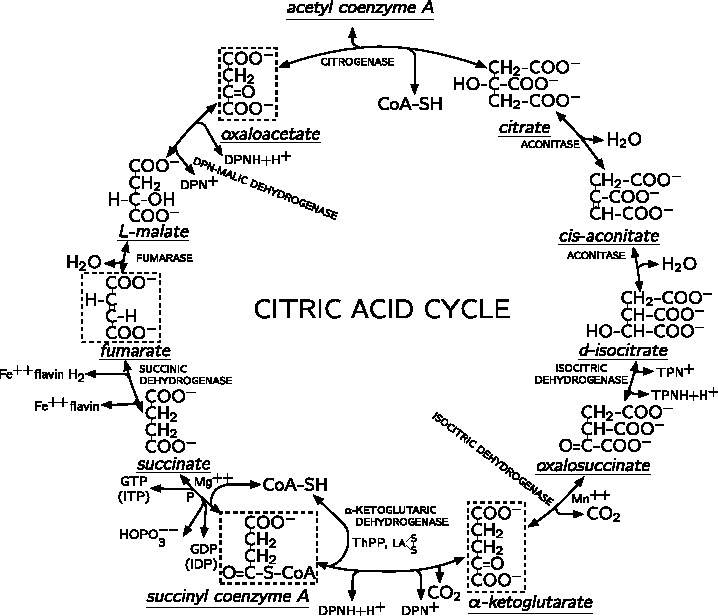
\includegraphics[width=0.5\textwidth]{Chapter3/克莱布斯循环}
    \caption{克莱布斯循环}
    \label{figure:克莱布斯循环}
\end{figure}

这里我们可以看到整整一系列分子,它们在一连串相当小的步骤组成的循环中从一个变到另一个。这个循环称为克莱布斯(Krebs)循环或呼吸循环。如果从分子发生的变化来说,每一种化合物和每一步反应都是相当简单的,但是——这是生物化学中非常重要的发现——这些变化\uwave{在实验室里比较难以完成}。假如我们有一种物质,还有另一种十分类似的物质,那么前一种物质并不就转变成后一种物质,因为这两种形式通常由一个能量屏障或“势垒”隔开。考虑这样一个类似的情况:如果我们要把一个物体从一个地方拿到另一个地方,而这两个地方处在相同的水平高度,但是分别在一座小山的两边,那么我们可以把物体推过山顶,但是要做到这一点需要一些附加的能量。由于这种原因,大多数化学反应都不会发生,因为有一种所谓的\uwave{活化能}妨碍这一反应的进行。为了在一种化合物中增加一个额外的原子,就要使这个原子靠得足够\uwave{紧},以便能出现某种重新排列;这样它就结合到那个化合物上去了。但是如果我们不能给它足够的能量使之靠得足够地近,它就不会越过势垒。只是上去了一部分路程后又倒退回。然而,假如我们真的能把分子拿在手中,把其中的原子推来推去使它出现一个缺口,让新原子进入,然后又使缺口一下子合拢,我们就找到了另一个办法,即\uwave{绕过}势垒,这不需要额外的能量,因此反应就较容易进行。现在,在细胞里确实\uwave{存在}着一些很大的分子,比起我们对其变化刚描写过的分子要大得多,它们以某种复杂的方式使较小的分子具有恰当的状态,从而使反应易于发生。这些很大的、复杂的分子称为\uwave{酶}。(它们起先被叫作酵素,因为原来是在糖发酵时发现的。事实上克莱布斯循环的某些反应最初就是在发酵中发现的。)由于有酶存在,反应就会进行。

酶是由另一种称为\uwave{蛋白质}的物质制成的。酶是非常大而复杂的,每一种酶都不同,并且都控制着一定的特殊反应。图3-1中每个反应中都写上了酶的名称。(有时同一种酶可以控制两种反应。)我们要强调指出:酶本身并不直接参与反应。它们并没有变化,只是使一个原子从一个地方跑到另一个地方。干完了这件事后,它又准备对下一个原子做同样的事,犹如工厂里的机器一样。当然,必须对某种原子进行补充,并且可以处理另一些原子。比如,以氢为例,有些酶具有特殊的结构单元,能在各种化学反也中运送氢原子。例如有3种或4种脱氢酶在我们整个循环的各个地方都用到。有趣的是,使一个地方的某些氢原子释放的机构将取走这些氢原子,并用到其他的地方去。

图3-1的循环中最重要的是GDP转变为GTP(二磷酸鸟嘌呤核苷变为三磷酸鸟嘌呤核苷),因为GTP比GDP含有更多的能量。就像在某些酶中存在着一种运送氢原子的“盒子”一样,在酶中也有特殊的携带能量的“盒子”,三磷酸基就是这样的“盒子”。 所以GTP比GDP具有更多的能量,而且如果循环是朝某个方向时,我们就产生具有附加能最的分子,它可以推动另一个需要能量的循环,比如肌肉的收缩。陈非存在着GTP,肌肉就不会收缩。我们可以拿几根肌肉纤维,把它们浸到水里,加一些GTP,只要这里存在着适当的酶,肌肉纤维就会收缩,GTP就变为GDP。所以真实的系统是在GDP-GTP转变中;在晚上就用白天贮藏起来的GTP使整个循环往另一个方向进行。你们可以看到酶对反应进行的方向并不介意,因为假如不是如此,就会违反一条物理定律。

物理学对于生物学和其他科学之所以极为重要还在于另一个原因,这与\uwave{实验技术}有关。事实上,如果不是由于实验物理的巨大发展,这些生物化学的循环图今天就不可能知道。其理由是:分析这种极其复杂的系统的最有效的方法就是要\uwave{辨认}在反应过程中所用到的原子。例如,如果我们能把一些带有“绿色标记”的二氧化碳引到循环中去,然后测量3秒钟后绿色标记的位置,在10秒钟后再测量一次,等等,我们就能描绘出反应的过程。那么“绿色标记”是什么呢?它们是同位素。我们可以回顾一下:原子的化学性质是由电子的数量而不是原子核的质量所决定的。但是有这种可能,比如在碳中,可能有6个或7个中子与每个碳原子核都具有的6个质子在一起。这两个原子C12与C13在化学上是相同的,但它们的重量不同,在核的性质上也有差别,因而是可以区别的。利用这些不同重量的同位素,或者甚至利用放射性同位素,如C14就有可能跟踪反应的过程,这是比较灵敏的探查极少量物质的方法。

现在,让我们回到酶和蛋白质的描述。并不是所有的蛋白质都是酶,但是所有的酶都是蛋白质。蛋白质有许多种,比如肌肉中的蛋白质、结构蛋白质,它们存在于软骨、头发和皮肤中,等等,这些蛋白质本身并不是酶。但是,蛋白质是生命的非常具有代表性的物质:首先,它们组成了所有的酶;其次,它们构成了大部分其余的生命物质。蛋白质具有十分有趣而简单的结构。它们是一系列,或者说是一链不同的氨基酸。有20种不同的氨基酸,它们全部都能互相组合而形成链,其骨架是CO--NH,等等。蛋白质不是别的,正是这20种氨基酸形成的各种各样的链。每一种氨基酸可能起某种特定的作用。比如,有一些氨基酸在一定的位置上有一个硫原子;当同一蛋白质内有两个硫原子时,他们就形成一个键,也就是说,他们把链在这两点上连接起来形成一个环。另一种氨基酸有一个额外的氧原子,因而使它变为酸性物质,再有一种则是碱性的特征。有些氨基酸在一边悬挂着一个大基团,因此占有许多空间。有一种称为脯氨酸的氨基酸实际上并不是氨基酸,而是亚氨基酸。这里稍微有些差别,因为当脯氨酸在链上时,就会出现扭曲。如果我们想制造一种特殊的蛋白质,就应当按照这样的规则:这里先放一个硫钩;然后加进某种东西来占据空位;再加入某种东西以形成链上的扭曲。这样,我们将得到一个外观上复杂的链,它们相互钩连在一起,具有某种复杂的结构;这可能就是所有的酶形成的方式。1960年以来,我们所获得的伟大成就之一就是终于发现了某些蛋白质的原子的精确空间排列。在这些蛋白质中,一条链上就含有56个或60个左右的氨基酸链,在两种蛋白质的复杂图样中已经确定了1000个以上的原子(如果把氢原子计入,那么就很接近于2000个)的位置。第一种阐明结构的蛋白质就是血红蛋白。这个发现的不足之处是我们从这样的图样中不能看出任何东西;我们不理解他为什么会具有那样的功能。当然,这是下一步需要解决的问题。

\begin{wrapfigure}{l}{0.4\textwidth}
    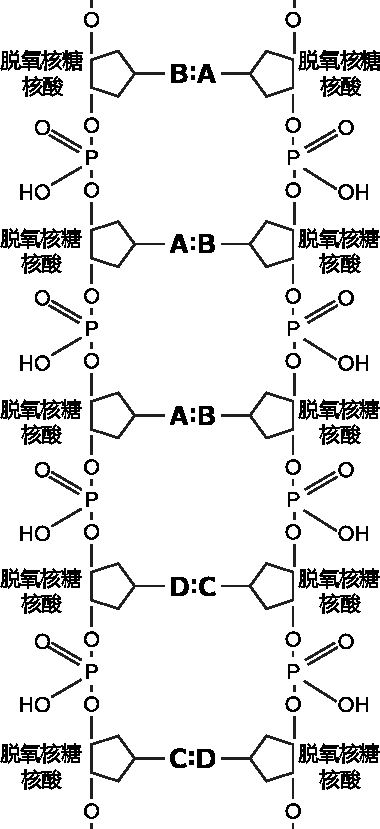
\includegraphics[width=0.35\textwidth]{Chapter3/部分DNA分子结构图}
    \caption{部分DNA分子结构图}
    \label{figure:部分DNA分子结构图}
\end{wrapfigure}
另一个问题是,酶怎么知道该成为什么?一个红眼蝇会生出一个小红眼蝇,这样产生红色素的整个酶组信息必定从一代传到下一代。这是由细胞核中的一种称为DNA(脱氧核糖核酸的缩写)的物质所完成的,它不是蛋白质。这种关键的物质从一个细胞传到另一个细胞(例如,精子细胞主要由DNA组成),并且携带了关于如何形成酶的信息。DNA是一张“蓝图”。那么这张蓝图看来象什么,他又如何起作用?首先,这张蓝图必须能加以复制。其次,它必须能给蛋白质以指令。说到复制,我们可能会认为这种过程像细胞的复制。但细胞只是简单地长大,然后一分为二。那么DNA分子也必须如此吗?他们也是长大以后一分为二吗?每一个\uwave{原子}当然不会长大并一分为二!因此,除非有一种更聪明的办法,否则就不可能复制出一个分子来。

对DNA这种物质的结构已经进行了很长时间的研究,首先用化学方法找出它的成分。然后又用X射线法找出它在空间的图像。结果得到如下值得注意的发现:DNA分子是一对彼此缠绕在一起的链。这些链与蛋白质的链类似,但化学结构上是完全不同的,每条链的骨架是一列糖与磷酸基,如图3-2所示。现在我们看出链是怎样容纳指令的,因为如果我们把这个链从中间劈开,就可以得到一个BAADC……系列,而每个生命体都可以有一个不同的系列。这样,也许为制造蛋白质所需的特殊指令已以某种方式包括在DNA的特殊系列里。

与链上的每一个糖相结合,并把两条链连接在一起的是一些交叉链对。然而他们并不都是相同的。总共有四种:腺嘌呤、胸腺嘧啶、胞嘧啶及鸟嘌呤。现在让我们称他们为A、B、C和D。有趣的是,只有一定的配对才能彼此处于相对的位置,例如A对B,C对D。当这些对放在二列链上时,他们“彼此对合”,并具有强大的相互作用能。然而C不适合于A、B也不适合于C;它们的适合配对是A对B,C对D。所以假如有一个是C,另一个就一定是D,等等。在一条链上无论是什么字母,在另一条链上则必须有特定的与之配对的字母。

那么,复制又是怎么一回事呢?假设我们把这个整链一分为二,我们怎么能制造出另一个正好与它一样的链呢?如果在细胞的物质中有一种加工部门,产生了磷酸盐、糖以及没有联在一个链上的A、B、C、D单元,那么唯一能与我们那个分开的链相连的单元必须是正确的,是BAADC……的补体,即ABBCD……。于是,当细胞分裂时,链亦从中间裂开,一半最终与其中一个细胞在一起,而另一半则留在另一个细胞内;当它们分离后,每个半链都会形成一个新的补足的链。

接下来的一个问题是A、B、C、D单元的次序究竟怎样精确地决定蛋白质中氨基酸的排列?这是今天生物学中没有解决的一个中心问题。然而,初步的线索,或者说一点信息是:在细胞中存在一种叫做微粒体的小小粒子,现已知道它就是制造蛋白质的地方。但是微粒体并不在细胞核内,而DNA及它的指令却在细胞核内。看来是有某种原因的。然而,现在也知道从DNA分出的小分子,不像携带有全部信息的大DNA分子那样长,而像它的一个小部分。它叫RNA,但这无关紧要。RNA是一种DNA的拷贝——一个简短的拷贝。RNA不知怎么地携带了关于要制造那种蛋白质信息,跑到微粒体中,这一点我们已经知道了。当它到达那里后,在微粒体中就合成出蛋白质,这一点也已经知道了。不过,氨基酸是怎样进入蛋白质的,又是怎样根据RNA上的密码来排列,等等,这些细节则还不太清楚。我们不知道如何去解这种密码。比方说,假如我们知道了一排字母ABCCA,我们也无法告诉你要制造的是什么蛋白质。

今天,无疑没有一个学科或领域在这样多的前沿上比生物学取得更大的进展;如果我们要作出引导着人们在探索生命的努力中不断前进的最有成效的假说,这就是:\uwave{所有的物} \uwave{质都是由原子组成的},并且生命体所做的每一件事都可以从原子的摆动和晃动中来理解。


\section{天文学}

在我们对整个世界非常概括的描绘中,现在必须转到天文学上。天文学是一门比物理学古老的学科。事实上,正是天文学向物理学提出了解释星体运动的如此美妙而又简单的问题,对于这个问题的理解,就构成了物理学的\uwave{开端}。但是在所有的天文学发现中,最值得注意的是:\uwave{星体是用同地球上一样的原子组成的}\footnote{在这里我是讲得多么匆促啊!在这个简短的叙述中,每一句话包含了多么丰富的内容!“星体和地球部是用同样的原子组成的。”我通常挑选跟这一样的小题目来讲课。据诗人们说,科学使星星失去了美丽——它们只不过是由气体原子组成的球体。但事实上根本不是这么一回事。我同样会在荒凉的夜晚仰望星空,并且有所感受。但我是看得太少了还是太多了呢?无垠的天空丰富了我的想象,我那小小的眼睛扫遍这回转的天穹,就能注视这欢乐的天空,并且能够捕获一百万年前发出的里光。宇宙是一幅无边无际的图案——我也是其中的一部分——也许组成我的身体的材料正是从某个已被遗忘的星球上喷射出来的,就像那儿的一个星球正在不断爆发一样。假若我通过帕洛玛(Palomar)的巨大眼睛[指安装在美国威尔逊(Wilson)山帕洛玛天文台的200英寸光学望远镜——译者注。]来观察夜空,那么就会看到原来或许紧靠在一起的星群从某个共同的起点往四面八方奔驰而去。宇宙的模式,或者说它的含义,它的\uwave{成因}是什么?人们对这些问题有点了解是不会有损于宇宙的奥秘的。真理远比以往任何艺术家的想象更为奇妙!为什么现在的诗人不去歌颂它?如果朱庇特(木星)像一个人,诗人就会歌颂它,但是如果朱庇特是一个由甲烷和氨组成的旋转的巨大球体,诗人就很可能默不作声。}。那么这是怎么知道的呢?原子释放具有确定频率的光,这有点像乐器的音色是具有确定的音调或频率的声音。当我们听见几种不同的音调时,可以分别说出它们来,但是当我们用眼睛观察混合的颜色时,却无法说出它由哪几种颜色组成,因为眼睛的辨别能力在这一点上远远比不上耳朵。然而,利用分光镜我们\uwave{可以}分析光波的频率,这样就可以看见各个不同星体上的原子所发生的真正“音调”。事实上,有两种化学元素在地球上被发现之前就已经在星体上发现了。氦是在太阳上发现的,它的名称就是由此而来的;锝是在一种冷却的星体上发现的。这当然使我们在理解星体方面取得了一定的进展,因为它们也是用跟地球上同样的原子组成的。今天,我们已经知道了许多有关原子的知识,特别是它们在高温而密度不太大的条件下的行为,这样我们就能用统计力学的方法来分析星体物质的性能。即使我们无法在地球上复现有关的条件,但是应用基本的物理定律往往能精确地或十分接近地说出会发生什么事情。这就是物理学帮助了天文学。看来令人奇怪的是,我们对太阳内部物质的分布情况的了解远胜于对自己脚下的地球内部情况的了解。我们对星体\uwave{内部}发生的情况的了解要比在人们必须通过望远镜来观察小小的光点这种困难的情况下可能推测出更多一些,因为在大多数情况下,我们可以\uwave{计算}出星体里的原子应当做些什么。

给人印象最深的发现之一是使星球不断发出光和热的能量来源问题。有一个参与这项发现的人,在他认识到要使恒星发光,就必须在恒星上不断地进行核反应之后一天晚上和他的一位女朋友出去散步。当这个女朋友说:“看这些星星闪烁得多美啊!”他说:“是的,在此刻我是世界上唯一知道\uwave{为什么}它们会发光的人。”他的女朋友只不过对他笑笑。她并没有对于同当时唯一知道恒星发光原因的人一起散步产生什么深刻的印象。的确,孤单是可悲的,不过在这个世界上就是这个样子。

正是氢原子核的“燃烧”给太阳提供了能量,这时氢也就转变成了氦。而且,最终从氢制造出各种化学元素的过程是在恒星的中心进行的。组成\uwave{我们}身体的各种元素在一个星体上一次“烹调”好后,就被抛出,存在于宇宙之中。我们是怎么知道的呢?因为这里有一条线索。\uwave{化学}反应永远改变不了不同的同位素的比例——多少\chemfig{C^{12}},多少\chemfig{C^{13}}等等,因为化学反应对二者而言都是大致相同的。这个比例纯粹是\uwave{核}反应的结果。看看,在熄灭的、冷却的余烬——比如我们自己就是这样的产物——里同位素的比例,就可以发现在构成我们身体的材料的形成时期\uwave{熔炉}象什么样子。这个熔炉很象恒星,所以很可能我们的元素是在恒星上“制造”出来,而在我们称为新星和超新星的爆炸中被喷吐出来的。正是因为天文学与物理学是这样密切相关,所以我们学下去时将要研究许多许多有关天文学的知识。



\section{地质学}

我们现存转到所谓的\uwave{地球科学}或\uwave{地质学}。首先是气象学和天气。当然气象学的\uwave{仪器}是物理仪器,就像前面所说的那样,实验物理学的发展使得提供这些仪器成为可能。然而,物理学家从来没有得出满意的气象学理论。“怎么!”你们会说:“这里除了空气以外什么东西都没有,而我们已经知道了空气的运动方程。”我们的确知道。“那么,如果我们知道了今天的空气状态,为什么就不能计算出明天的空气状态?”首先,我们并不\uwave{真正}知道今天的状态究竟是怎样的,因为空气到处旋转。结果它非常敏感,甚至不稳定。假如你们看到过水流平稳地流过水坝,然后当它下落时一下子变成大量的水珠和水滴的话,你就会懂得我所说的不稳定是什么意思了。你们知道水在流出溢水口之前的情况,它是十分平滑的;但是在它开始下落的一瞬间,水滴从哪里开始溅出?水滴将会有多大,并且在哪里的因素是什么?这些都无法知道,因为这里水是不稳定的。而对于空气来说,即使是平稳地运动着,但当它越过一座山时就变成了复杂的旋涡。在许多领域中都出现这种\uwave{湍流}现象,我们在今天还无法对之进行分析。现在,赶快离开天气问题,回到地质学上去吧!

对于地质学而言,它的基本问题是,究竟是什么使地球成为现在这个样子?最明显的过程就在你们眼前,这就是河流、风等等的侵蚀过程。要理解这些事是相当容易的,但是要知道,对于每一片侵蚀都有等量的另外一些东西出现。平均而言,今天的山脉并不比过去的低,因此必定有一种\uwave{造}山过程。假如你们学过地质学,你们就会知道,确实\uwave{存在}着造山过程以及火山作用,这些现象没有人懂得,但却占了地质学的一半内容。实际上,火山的本质并没有被人们所理解。造成地震的原因是什么最终也不了解。我们所知道的是,如果一个东西推动另外一些东西,那么就会突然断裂,并且产生滑动,这当然是对的。但是什么东西在推?为什么会这样?有一种理论认为,在地球内部存在着环流,它是由于内外温度上的差别而造成的,也就是它们在运动过程中轻微地推着地球的表层。这样假如有两股相对的环流在某个地方碰上的话,物质就会在这个区域里堆积起来而形成山脉,这些山脉处于非常不相宜的受到应力的状态,这样就会引起火山爆发,造成地震。

那么地球内部的情况是怎样的呢?关于地震波在地球里的传播速度以及地球的密度分布已经了解得很多。然而,关于物质处于我们预期在地球中心所应有的压强之下会有怎样的密度,物理学家没有能够提出一种有效的理论。换句话说,我们还不能很好地解决在这种情况下的物质的性质问题。我们在地球方面所做的事比在星体的物质条件下所做的事要差得多。这里所包含的数学到现在为止看来似乎过于复杂,但是也许不要很长时间就会有人认识到这是一个重要的问题,并且真正着手于解决这个问题。当然,另一方面,即使我们确实知道了密度,还是不能判断环流,也不能真正得知高压下的岩石的性质。我们无法说出岩石要多快才会“融化”;这必须通过实验来解决。


\section{心理学}

接下来,我们考虑\uwave{心理}科学。顺便提一下,心理分析并不是一门科学,它充其量不过是一个医学过程,也许更像巫术。它有一个疾病起源的理论——据说有许多不同的“幽灵”等等。巫医有一个理论说像疟疾那样的疾病是由进入空气中的幽灵所引起的;但是医治疟疾的药方并不是将一条蛇在病人头上晃动,而是奎宁。所以,如果你的身体感到有什么不舒服,我倒劝你到巫医那儿去,因为他是对疾病知道得最多的那批人中的一个。然而,他的知识不是一种科学。心理分析没有用实验仔细地检验过,因此没有办法知道,在哪些情况下它是有效的,在哪些情况下则是无效的,等等。

心理学的其他一些分支,包括感觉的生理学——在眼睛里出现一些什么情况,在大脑中出现一些什么情况——可以说,是并不令人感到兴趣的。但是在它们的研究中取得了一些微小的然而是真正的进展。有一个最有趣的技术性问题可以归之为心理学,也可以不归之为心理学。即有关大脑——如果你愿意的话,或者说神经系统的中心问题是:当某种动物学到了某件事后,它就能做一些以前不会做的事,所以它的大脑细胞也一定会有变化——只要大脑细胞是由原子构成的。那么,\uwave{差别表现在哪里呢}?当一件事情被记在大脑里后,我们不知道在哪儿去找它,或者去找些什么东西。如果一件事情被学到了,它意味着什么,或者说神经系统有些什么变化,我们都不知道。这是一个很重要的问题,但根本没有解决。然而,假设存在着某种记忆的物质的话,那么大脑恰恰就是这么多的连线和神经的集合体,这种集合体大概是无法用简单的方式来分析的。这和计算机以及计算机单元很类似,它们也有大量的布线,有某种单元,大概就类似于神经元触点,或者说一根神经到另一根神经的联结点。思维和计算机之间的联系是一个非常有趣的课题,但我们在这里没有时间作进一步的讨论。当然,必须懂得这个课题在有关人们一般行为的真正复杂性上所告诉我们的东西是非常之少的。每个人之间存在着如此巨大的差别。为了要达到那种理解将需要很长的时间,我们必须把研究起点退到更后面的地方。假如我们总算能够解决\uwave{狗}是怎样活动的,我们就已经走得够远了。



\section{情况何以会如此}

为了使物理学不仅在仪器的发明方面,而且在\uwave{理论}方面对其他科学也有所裨益,有关的科学就必须向物理学家提供用物理学家的语言描述的研究对象。人们或许会问:“青蛙为什么会跳跃?”物理学家对此就回答不出。如果人们告诉他青蛙是什么,这里有这么多的分子,那里有神经,等等,情况就不同了。假如人们或多或少地告诉我们地球或者星星是怎样的,那么我们就能够把它们想象出来。要使物理理论有点用处,我们就必须知道原子的位置。要理解化学,就应当确切知道存在着哪些原子,不然就无法分析。当然,这只是限制因素之一。

在物理学的姐妹科学中存在着另一\uwave{种}物理学中不存在的问题,因为没有更好的措词,我们可以称它为历史问题。情况何以会如此?假如我们懂得了生物学的一切,就会想要知道现在地球上的所有生物是怎样发展的。这就是生物学的一个重要部分——进化论。在地质学中,我们不仅要知道山脉正在怎样形成,而且要知道整个地球最初是怎样形成的,太阳系的起源,等等。当然,这就会使我们想要知道在宇宙的彼时有什么样的物质。恒星是怎样演化的?初始状态又是如何?这些都是天体的历史问题。今天我们已经弄清楚许多有关恒星的形成及有关组成我们身体的元素的形成的知识,甚至还知道一些有关宇宙起源的事。

目前在物理学中还没有这种历史问题要研究。我们不会问:“这里是物理学的定律,它们是怎样变化而来的?”我们此刻不去想象物理定律以某种方式随时间而变化,不认为它们在过去与现在是有差别的。当然,不能排除这种\uwave{可能},而且我们一旦发现果真如此时物理学的历史问题就将与宇宙发展的其余历史问题交织在一起,于是物理学家就要谈论天文学家、地质学家和生物学家同样的问题。

最后,在许多领域中普遍存在着一个物理问题,这是一个很古老的问题,但是还没有得到解决。这并不是寻找新的基本粒子的问题,而是好久之前——大约一百多年前就遗留下来的一件事情。在物理学上没有一个人能够真正令人满意地对它进行数学的分析,尽管它对于姐妹科学来说是一个重要问题。这就是\uwave{环流}或\uwave{湍流}的分析。如果我们注视着一个恒星的演化,就会发现这样的情形,我们可以推断出将要出现对流,但在这以后我们就再也无法推断会有什么事发生了。几百万年后这个星体会发生爆炸,但是我们想不出是什么道理。我们不能分析气候,也不知道地球内部的运动。这类问题的最简单的形式就是取一根很长的管子,使水高速通过。我们问:使一定量的水通过管子需要多大的压力?没有人能从基本原理和水的性质出发来分析它。如果水流得非常慢,或者用的是蜂蜜那样的粘性物质,那么我们可以分析得很不错。在你们的教科书上就有这方面的内容。我们真正不能处理的是实际的水流过管子的问题。这是一个我们有朝一日应当解决的中心问题,但是现在还没有解决。

有一位诗人曾经说过:“整个宇宙就存在于一杯葡萄酒中。”我们大概永远不可能知道他是在什么含义上这样说的,因为诗人的写作并不是为了被理解。但是真实的情况是,当我们十分接近地观察一杯葡萄酒时,我们可以见到整个宁宙。这里出现了一些物理学的现象:弯弯的液面,它的蒸发取决于天气和风;玻璃上的反射;而在我们的想象中又添加了原子。玻璃足地球上的岩石的净化产物,在它的成分中我们可以发现地球的年龄和星体演化的秘密。葡萄酒中所包含的种种化学制品的奇特排列是怎样的?它们是怎样产生的?这里有酵素、酶、基质以及它们的生成物。于是在葡萄酒中就发现了伟人的概括:整个生命就是发酵。任何研究葡萄酒的化学的人也必然会像巴斯德(L.Pasteur)所做过的那样发现许多疾病的原因。红葡萄酒是多么的鲜艳!让它深深地留在人们美好的记忆中去吧!如果我们微不足道的有限智力为了某种方便将这杯葡萄酒——这个宇宙——分为几个部分:物理学、生物学、地质学、天文学、心理学等等,那么要记住大自然是并不知道这一切的。所以让我们把所有这些仍旧归并在一起,并且不要忘记这杯酒最终是为了什么。让它最后再给我们一次快乐吧!喝掉它,然后把它完全忘掉!


\chapter{能量守恒}

\section{什么是能量}

讲完对事物的一般性描述后,从这一章起,我们开始比较详细地研究物理学中各个方面的问题。为了说明理论物理学中可能用到的概念和推理的类型,我们现在来考查能量守恒定律,它是物理学:最基本的定律之一。

有一个事实,如果你愿意的话,也可以说一条\uwave{定律},支配着至今我们所知道的一切自然现象。没有发现这条定律有什么例外——就我们所知,它是完全正确的。这条定律称为\uwave{能量守恒定律}。它指出,在自然界所经历的种种变化之中,有一个称之为能量的物理量是不变的。那是一个最抽象的概念,因为它是一种数学原理;说的是在某种情况发生时,有一个数量是不变的。它并不是一种对机制或者具体事物的描写,而只是一件奇怪的事实。起先我们可以计算某种数值,当我们看完了大自然耍弄的技巧表演后,再计算一次数值,其结果是相同的。(有点类似于在红方格中的象,移动了几步后——具体步骤并不清楚——它仍然在某个红方格里。我们这条定律就是这种类型的定律。)由于这是一种抽象的概念,我们将用一个比喻来说明它的含义。

设想有一个孩子,或许就叫他“淘气的丹尼斯(Dennis)”,他有一堆积木,这些积木是绝对不会损坏的,也不能分成更小的东西。每一块都和其余的相同。让我们假定他共有28块积木。每天早上他的母亲把他连同28块积木一起留在一个房间里。到了晚上,母亲出于好奇心很仔细地点了积木的数目,于是发现了一条关于现象的规律——无论丹尼斯怎样玩积木,积木数目仍旧是28块!这种情况继续了好几天。直到有一天她发现,积木只有27块了,但是稍许调查一下就发现在地毯下面还有一块——为了确信积木的总数没有改变,她必须到处留神。然而,某一天积木的数目看来有些变化,只有26块了!仔细的调查表明:窗户已经打开,再朝窗外一看,就发现了另外的两块积木。又有几天,经过仔细的清点表明总共有30块积木!这使她相当惊愕,以后才了解到布鲁斯(Bruce)这个孩子曾带着他的积木来玩过,并留了几块在丹尼斯的房间里。自从丹尼斯的母亲拿走了多余的积木,把窗关上,并且不再让布鲁斯进来以后,一切都很正常,直到有一次,她清点时发现只有25块积木。然而,在房间里有一个玩具箱,母亲走过去打开这个箱子,但是孩子大声叫喊道:“不,别打开我的箱子,”不让她打开玩具箱。这时母亲十分好奇,也比较机灵,她想出了一种办法,她知道—块积木重3英两,有一次当她看到积木有28块时曾经称过箱子的重量为16英两,这一次她想核对一下,就重新称一下箱子的重量,然后减去16英两,再除以3,于是就发现了以下的式子:
\begin{equation}
    \label{Eq:I:4:1}
    \text{(所见到的积木数)}
    +
    \frac{\text{(箱重)}-\text{$16$ 英两}}{\text{$3$ 英两}}=
    \text{常数}.
\end{equation}
接着,又好像出现了某种新的偏差,但是仔细的研究又指出,浴缸里的脏水的高度发生了变化,孩子正在把积木扔到水里去,只是她看不见这些积木,因为水很混浊,不过在她的公式里再添上一项她就可以查明在水中有几块积木。由于水的高度原来是6英寸,每一块积木会使水升高$1/4$英寸,因而这个新的公式将是:
\begin{align}
    \label{Eq:I:4:2}
    \text{(所见到的积木数)}
    +
    \frac{\text{(箱重)}-\text{$16$ 英两}}{\text{$3$ 英两}}
    \frac{\text{(水的高度)- $6$英存}}{\text{$1/4$ 英寸}}+
    =
    \text{常数}.
\end{align}
在她这个复杂性逐渐增加的世界里,她发现了—系列的项来表示计算积木的方法,这些积木藏在不准她去看的那些地方。结果,她得出了\uwave{一个用于计算数量}的复杂公式,无论孩子怎样玩耍,这个量总是不变的。

这件事情和能量守恒有什么相似的地方呢?抽象地说,必须从这个图像中除去的最显著的一点就是,\uwave{根本没有积木}。在(\ref{Eq:I:4:1})及(\ref{Eq:I:4:2})中取走第一项,我们就会发现自己是在计算多少是有点抽象的东西。上述比较的相似之处在于以下几点。第一,当我们计算能量时,有时其中的一部分离开系统跑掉了,有时又有另一些能量进入这个系统。为了验证能量的守恒,必须注意我们没有把能量引入系统中或从系统中取走能量。第二,能量有许多\uwave{不同的形式},对每一种形式都有一个公式。这些不同形式的能量是:重力势能、动能、热能、弹性能、电能、化学能、辐射能、核能、质能。假如我们把表示这些能量的公式全都加在一起,那么,除非有能量逸出或有其他能量加入,否则其总和是不会改变的。

重要的是要认识到:在今天的物理学中,我们不知道能量究竟\uwave{是}什么。我们并不把能量想象成为以一定数量的滴状形式出现。它不是那样的。可是有一些公式可以用来计算某种数量,当我们把这些数量全部加在一起时,结果就是“28”——总是同一个数目。这是一个抽象的对象,它一点也没有告诉我们各个公式的机制或者\uwave{理由是}什么。


\section{重力势能}

只有当我们的公式包含了所有形式的能量时才能理解能量守恒。我想在这里讨论一下地球表面附近的重力势能的公式,并用一种与历史无关的方式来导出这个公式,这种推导方式只是为这堂课想出来的,也就是说一种推理思路,为的是要向你们说明一个值得注意的情况:从几个事实和严密的推理出发可以推断出很多有关大自然的知识。它也表明了理论物理学家投身于怎样的一类工作,我们这里的推理仿照了卡诺(Carnot)讨论蒸汽机效率时所使用的极其杰出的论证方式\footnote{事实上你们可能已经知道式(4.3),因此这一讨论的意义与其说是得出(4.3)式,不如说是表明能用推理论证的方法来得出这样的结果。}。

让我们考虑一种起重的机械,它有这样的特点:用降低一个重物的方法来提高另一个重物。此外还假设:在这种起重机械中\uwave{不可能有永恒的运动}。(事实上,根本不存在什么永恒运动,这正是能量守恒定律的一般表述。)在定义永恒运动时必须特别小心。首先,我们定义起重机械的永恒运动, 假如我们提起和放下一些重物并使机械回复到原来的状态后,发现最后的结果是\uwave{提升了一个重物},于是我们就有了永恒运动的机械,因为我们可以利用被提起的重物使另外的一些东西运转。这就是说,提起重物的机械\uwave{精确地}回到\uwave{原来的状态},而且是完全独立完成的——它没有从外界(就像布鲁斯的积木那样)取得能量来抬高这个重物。

图4.1所示是一台很简单的起重机械。这台机械举起三个单位的重物。我们把这三个单位的重物放在一个秤盘里,在另一个盘内则放置一个单位的重物。但是,为了使机械实际上能工作,我们必须在左边减去一点点重量。另一方面,我们可以通过降低三个单位的重物来升高一个单位的重物,只要我们在右边的盘子里提起一点点重量,当然,我们认识到,对于任何\uwave{实际}的起重机械来说,为了使它运行必须施加一点额外的作用。这一点我们暂时不去考虑。理想的机械并不需要额外的作用,然而它们事实上是不存在的。我们实际使用的机械在某种含义上可以说\uwave{几乎}是可逆的,即假如降低一个单位的重物能使这种机械提升三个单位的重物的话,那么降低三个单位的重物也能使这种机械把一个单位的重物提升到接近原来的高度。

\begin{wrapfigure}{r}{0.4\textwidth}
    \centering
    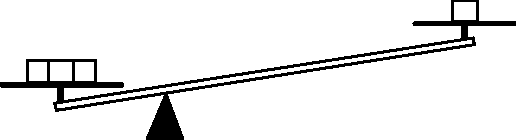
\includegraphics[width=0.35\textwidth]{Chapter4/简单的起重机械}
    \caption{简单的起重机械}
    \label{figure:简单的起重机械}
\end{wrapfigure}

我们设想存在着两类机械:一类是\uwave{不}可逆的,它包括所有的真实的机械;另一类是可逆的。当然实际上它是不可能达到的,不管我们怎样仔细地去设计轴承、杠杆等等。但是,我们假设有这样的东西——一台可逆机;在它使一个单位(一磅或任何其他单位)重的物体降低一个单位距离的时候提起了三个单位的重物。把这台可逆机称为A机。假定它使三个单位的重物升高的距离是$ x $。此外,假设还有另一台机械——B机,它不一定是可逆机,并且也使一个单位的重物降低一个单位距离,不过使三个单位的重物升高的距离是$ y $。我们现在可以证明$ y $不会高于$ x $,这就是说,不可能建造这样一种机械,能把重物抬得比可逆机所提到的高度还要\uwave{高}。让我们来看看为什么是这样。假设$ y $大于$ x $。我们用B机使一个单位的重物降低一个单位距离,这使三个单位的重物升高距离$y$,然后,我们可以使这个重物从$ y $降到$ x $获得\uwave{自由的能量},再利用可逆机A反向运转,使三个单位的重物降低$ x $而使一个单位的重物升高一个单位距离。这样一个单位的重物回到了原来的高度,而使这两台机械又处于初始的备用状态!因此,假如$ y $高于$ x $,那么就会有永恒运动,但我们已经假设这是不可能的。于是利用这些假定,我们就能够推导出\uwave{$ y $不会比$ x $}高,因此在所有可能设计的机械中,可逆机是最好的。

我们还可以看出所有的可逆机提升的高度一定\uwave{完全相同}。假定B的确也是可逆的。当然,前面关于$ y $不会高于$ x $的论据现在同样成立,但是我们也可以把这两台机械的工作顺序倒过来,即反之论证$ x $不高于$ y $。这一点是很值得注意的,因为它使我们能够在\uwave{不考察内部机制}的情况下分析不同的机械对物体可以提升的高度。我们立刻知道,如果有一个人制作了一组极其精巧的杠杆,利用这组杠杆使一个单位的重物降低一个单位距离就可以把三个单位的重物提升到某一个高度,把这组杠杆和一个具有同样用途的简单的可逆的杠杆作比较就可以知道它不会比简单的可逆的杠杆提得更高,而是或许还会低一些。假如这个人的机械是可逆的,我们也能精确地知道它可以提得\uwave{多}高。概括地说就是:每一台可逆机械无论怎样运转,当它使一个单位的重物下降一个单位距离时,总是会使三个单位的重物提升同样的距离$ x $。很清楚,这是一条非常有用的普遍定律。接下来的问题自然是$ x $是多少?

\begin{wrapfigure}{l}{0.45\textwidth}
    \centering
    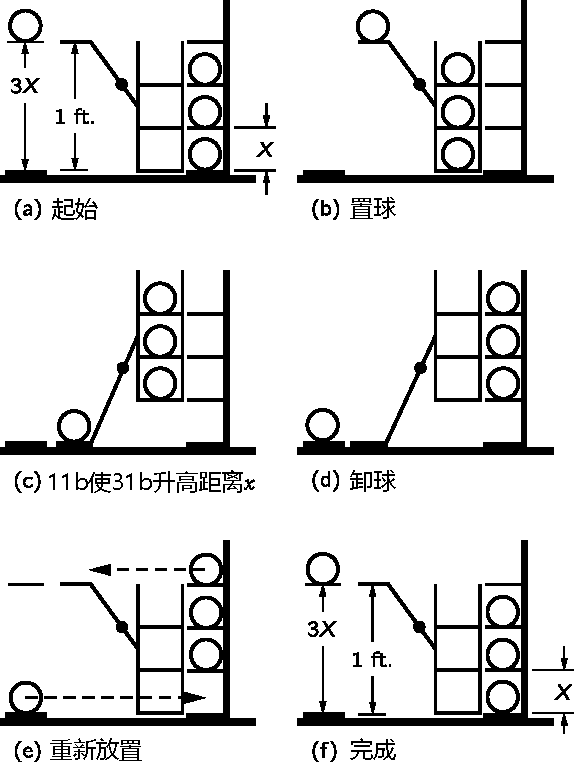
\includegraphics[width=0.42\textwidth]{Chapter4/一种可逆机}
    \caption{一种可逆机}
    \label{figure:一种可逆机}
\end{wrapfigure}

假如我们有一台可逆机,它能在3对1时提升距离$ x $。在图4.2中,我们在一个固定的多层架子上放置三个球。另外有一个球放在离地面一英尺的台上。这台机械可以使一个球降低1英尺来抬高三个球。现在,我们来这样安排:设容纳三个球的升降台有一层底板和两层架子,间隔正好是$ x $,其次,容纳球的多层架的间隔也是$ x $(图a)。首先我们使小球从多层架水平地滚到升降台上的架子中去(图b),我们假设这并不需要能量,因为高度并没有改变。于是开动可逆机进行工作:它使一个球降到底层,而使升降台升高距离$ x $(图c)。由于我们已经巧妙地安排了多层架,于是这些球又和架子相平。这样就把球卸到了多层架上(图 d)。卸了球以后,我们可以使机械回复到初始状态。现在在上面三层架子上有三个球,在底部有一个球,但是奇怪的是从某种观点上讲,我们根本没有使其中\uwave{两}个升高,因为,无论如何第二层和第三层架子像以前一样里面装着球。因此,最后的效果是使\uwave{一个}球升高了$ 3x$的距离。假如$  3x $超过1英尺,那么我们就可以把小球\uwave{放下来}使机械回到初始状态(图f),这样就能使这个装置再次运转。所以$ 3x $不可能超过1英尺,因为如果$ 3x $超过1英尺;我们就能创造出永恒运动。同样,使整台机械反向运行,我们可以证明,\uwave{1英尺不能超过$ 3x $},因为这是一台可逆机。所以\uwave{$ 3x $既不大于也不小于 1英尺},这样我们只是通过论证就发现了一条规律,$x=1/3$英尺。显然,这条规律可以推广为:开动一台可逆机使1磅重物降下一定距离,那么这台机械可以使$p$磅重物提高那段距离的$1/p$。另一种表示结果的说法是:3磅乘以所提高的距离(在我们的问题中是$ x $),等于1磅乘以所降低的距离(在这种情况下是1英尺)。如果我们先把所有的球的重量分别乘以它们现在所在的高度,然后使机械运转,再把所有的球的重量乘以它们所在的高度,得出的\uwave{前后结果不会有任何改变}。(我们必须把例子中只移动一个重物的情况推广到当我们降低一个重物就能提升几个不同的重物的情况——但这是不准的。)

我们把重量和高度的乘积之和称为\uwave{重力势能}——这是一个物体在空间上与地球之间的相互关系而具有的能量。那么,只要我们离地球不是太远(当位置很高时重力要减弱),重力势能的公式就是
\begin{equation}
    \label{Eq:I:4:3}
    \text{(一个物体的重力势能)}=
    \text{(重量)}\times\text{(高度)}
\end{equation}
这是一条十分优美的推理思路。唯一的问题在于,或许这并不是实际的情形。(无论如何,大自然\uwave{毋须}按我们的推理行事。)例如,也许永恒运动事实上是可能的。某些假设可能是错误的,或者我们的推理或许有错误,所以验证总是必要的。事实上,实验证明它是正确的。

那种与别的物体的相对位置有关的能量的一般名称就称为\uwave{势能}。当然,在上面的特殊情况中,我们则称它为\uwave{重力势能}。如果我们克服电力做功,而不是克服重力做功,即用许多杠杆“提升”一些电荷使之离开其他的电荷,那么所包含的能量就称为电势能。一般的原则是能量的变化为有关的力乘以力所推过的距离,而且这是一般的能量变化:
\begin{equation}
    \label{Eq:I:4:4}
    \text{(能量的变化)}=
    \text{(力)}\times\text{(力在作用下所通过的距离)}
\end{equation}
随着课程的进展我们还要讲到其余的种种势能。

\begin{figure}[htbp]
    \centering
    \begin{minipage}[t]{0.4\textwidth}
        \centering
        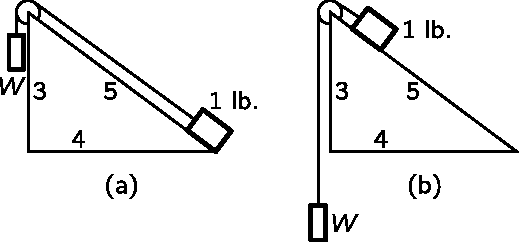
\includegraphics[width=6cm]{Chapter4/斜面}
        \caption{斜面}
    \end{minipage}
    \begin{minipage}[t]{0.4\textwidth}
        \centering
        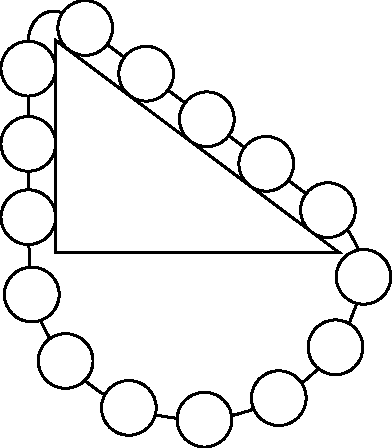
\includegraphics[width=6cm]{Chapter4/斯蒂维纽司的墓志铭}
        \caption{斯蒂维纽司的墓志铭}
    \end{minipage}
\end{figure}

在许多情况下能量守恒原理对于推断会发生什么事都是非常有用的。在高中你们已学过许多有关不同用途的滑轮和杠杆的定律,我们现在可以看到所有这些“定律”\uwave{都是一} \uwave{回事},并且不需要记住75条法则。一个简单的例子是如图4.3所示的一个光滑斜面,很巧,这是一个3--4--5的三角形。我们在斜面上用滑轮挂上一个1磅重的物体,而在滑轮的另一端悬挂一个重物$ W $。我们想知道为了平衡在斜面上的1磅重物,$ W $必须是多重?怎样来求出答案呢?假如我们说情况正好是平衡的话,那就是可逆的,因而可以使重物上下移动。所以,我们可以考虑下述情况。起初,如图(a)所示,1磅重物在斜面底部,而重物$ W $在斜面的顶端。当$ W $以一种可逆的方式滑下去后,1磅的物体就在斜面顶部,而$ W $经过的距离就是斜边的长度,如图(b)所示,即5英尺。我们使1磅重的重物只\uwave{提高}了3英尺而使W降低了\uwave{5英尺},所以,$ W=3/5 $磅。注意,我们是从\uwave{能量守恒},而不是从力的分解来得出这个斯蒂维纽司(Stevinus)所发现的方法就铭刻在他的墓碑上。图4.4说明这个重物一定是$ 3/5 $磅,因为这个圆球链并没有转动,很明显链条的下端的部分是为自身所平衡的,所以一边三个重物的拉力必须与另一边五个重物的拉力平衡,即按边长的比例。从图中你们可以看到,$W$一定是$ 3/5 $磅。

\begin{wrapfigure}{l}{0.4\textwidth}
    \centering
    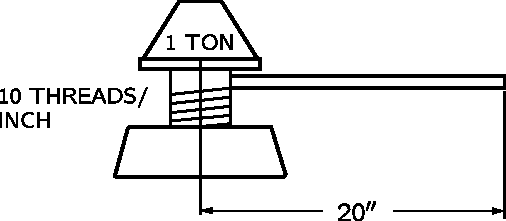
\includegraphics[width=0.35\textwidth]{Chapter4/螺旋起重器}
    \caption{螺旋起重器}
    \label{figure:螺旋起重器}
\end{wrapfigure}

让我们现在用图4.5所示的螺旋起重器这个比较复杂的问题来说明能量守恒原理。螺旋的把柄长为20英寸,螺纹为每英寸10圈,我们想知道,为了举起一吨(2000磅)的重物,在把柄上要施加多大的力?假如我们要使一吨重物升高1英寸,就必须使把柄转10圈。把柄转一次时大约走过126英寸。所以它总共要走过1260英寸,如果我们利用各种滑轮之类的机械,就可以用加在柄的端点上的一个未知的小重物$ W $来举起1吨的重物,我们发现,$ W $大约是1.6磅。这就是能量守恒的一个结果。

\begin{wrapfigure}{r}{0.4\textwidth}
    \centering
    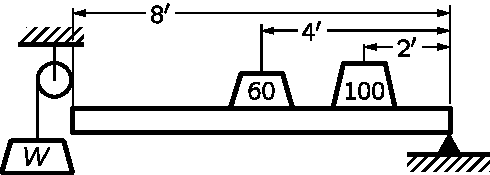
\includegraphics[width=0.35\textwidth]{Chapter4/一端支撑着的荷重杆}
    \caption{一端支撑着的荷重杆}
    \label{figure:一端支撑着的荷重杆}
\end{wrapfigure}

在图4.6中我们举一个稍为更复杂一点的例子。一根8英尺长的棒,一端被支撑着,在棒的中间有一个60磅的重物,离支点2英尺处有一个100磅的重物,假如不考虑棒的重量,为了保持它的平衡,我们要在棒的另一端加多大的力?假设在棒的那一端放上一个滑轮,并在滑轮上悬挂一个重物$ W $,为了使棒平衡,$ W $应当是多重?我们设想$ W $落下任意一段距离,为了简便起见,设它下降了4英寸,那么这两个重物要升高多少呢?棒的中心升高了2英寸,而离固定端2英寸处的那一点升高了1英寸,所以,各个重物与高度的乘积之和不变,这个原理告诉我们,$ W $乘以下降的4英寸,加上60磅乘以升高的2英寸,再加上100磅乘以升高的1英寸,其和必定是零。
\begin{equation}
    \label{Eq:I:4:5}
    -4W+(2)(60)+(1)(100)=0,\qquad
    W=\text{$55$ 磅}
\end{equation}
这就是说为了使棒平衡,必须加上一个55磅的重物。用这种方法,我们可以得出“平衡”定律——复杂的桥梁建筑的静力学,等等。这种处理问题的方法称为\uwave{虚功原理},因为为了进行这种论证,我们必须\uwave{设想}系统移动一下——即使它实际上没有移动,甚至不能移动。为了运用能量守恒的原理,我们用了很小的假想的运动。


\section{动能}

为了说明另一种形式的能量,我们来考虑一个单摆(图4.7)。假如我们把它拉向一边,再把它放开,它就会来回摆动。在这种运动中,每当从端点跑向中点时,它的高度降低了,这时势能跑到哪里去了呢?当摆降到底部时,势能就消失了,不过,它将再次爬上来。可见重力势能必定转变为另一种能量形式。很明显它是依靠了自己的\uwave{运动}才能重新爬上来。所以,当它到达底部时,重力势能就转变为某种其他形式的能量。

\begin{wrapfigure}{l}{0.4\textwidth}
    \centering
    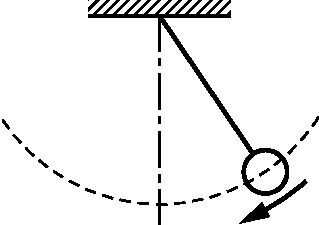
\includegraphics[width=0.35\textwidth]{Chapter4/单摆}
    \caption{单摆}
    \label{figure:单摆}
\end{wrapfigure}

我们应当得出一个运动能量的公式。现在,回想一下关于可逆机的论证,很容易看出,在底部的运动必定具有一定量的能量,可使摆升高到一定高度,这个能量与摆上升的\uwave{机制}无关,或者说与上升的路径无关,所以与我们对孩子玩积木的情形所写出的公式一样,这里也有一个(两种能量间的)等价公式。我们有另一种表示能量的形式,要说明它是不难的。摆在底部的动能等于重量乘以它能升高的高度:\text{K.E.}= WH。现在需要的是一个利用某种与物体的运动有关的规则来说明摆动高度的公式。假如我们以一定的速度直接朝上抛出一个物体,它将到达一定的高度;我们暂时还不知道到底是多高,但是它依赖于速度——关于这个,有一个相应的公式。于是,为了找到物体以速度$ V $运动的动能的公式,我们必须计算它能到达的高度;再乘以物体的重量。我们立刻就会知道,可以把动能写成这种形式:
\begin{equation}
    \label{Eq:I:4:6}
    K.E.=\frac{WV^2}{2g}
\end{equation}
当然,运动具有能量这个事实与物体处于重力场内这件事毫无关系。无论运动怎样产生,这都没有关系。这是一个适用于各种速度的一般公式。(\ref{Eq:I:4:3})及(\ref{Eq:I:4:6})两式都是近似的公式。(\ref{Eq:I:4:3})式在高度很大时是不正确的,因为这时,重力要减弱;而(\ref{Eq:I:4:6})在高速时要加以相对论性的校正。然而,当我们最后得到动能的精确公式时,能量守恒定律是正确的


\section{能量的其他形式}

我们可以继续以这种方法来说明能量还以其他的方式存在。首先考虑弹性能,假如我们拉伸弹簧,就必须作一些功,因为拉伸时,可以提起重物。所以弹簧在伸长的情况下具有做功的可能性。假如我们求出重量与高度的乘积之和,那将与总能量不符——我们必须加上另外的一些东西来说明弹簧处于拉紧状态这一事实。弹性能就是关于弹簧被伸长时这个事实的表述。它有多大呢?假如我们释放弹簧,那么弹簧经过平衡点时,弹性能就转变为动能,能量就在弹簧的伸长、压缩和动能之间来回变换。( 这里也有一些重力势能的增减,但是如果我们愿意的话,可以使实验“斜着”做)弹簧将一直来回振动,直到能量失掉为止……。啊哈!前面我们已经在整个过程中玩了一点小小的手法——如加上一些小重物使物体运动,或者说机械是可逆的,它们可以永远运动下去等。但是,我们可以看到这些东西最终都要停下来的。当弹簧不再上下振动时,能量到哪里去了呢?这就引进了另一种形式的能量:\uwave{热能}。

在弹簧或杠杆里有着由大量原子组成的晶体。假若极其仔细和精致地安排了机械的各个组成部分后,人们可以试着使事情作这样的调整:当某个东西在另一个东西上滚动时,根本没有一个原子会作任何跳动。但是我们必须非常小心。通常在机器运转时,由于材料本身的缺陷,会产生撞击和跳动,材料中的原子就开始无规则地摆动。于是那部分能量失踪了,但我们却发现机械运动减慢后,材料中的原子正以杂乱无章的方式摆动着,不错,这里仍然有动能,但是它与看得见的运动没有联系。多么奇怪!我们何以\uwave{知道}这里仍然有动能呢?我们发现,从温度计上可以看出,事实上弹簧或杠杆\uwave{变热}了,所以确实动能有了一定数量的增加。我们称这种形式的能量为\uwave{热能}。但是我们知道这实在并不是一种新的形式,它就是内部运动的动能。(我们在宏观范围内对物质所做的一切实验中都有一个困难,即不能真正演示出能量守恒,也不能实际制成可逆机,因为每当我们使大块材料运动时,原子不会绝对不受扰动,所以总有一定量的无规则运动进入原子系统,我们无法用眼睛看出这一点,但是可以用温度计或其他方式测量出来。)

还有许多其他形式的能量,当然,眼下不可能对它们叙述得更详细些。这里有电能,它与电荷的吸引和排斥有关。存在着一种辐射能,即光能,我们知道它是电能的一种,因为光可以表示为电磁场的振动;还有化学能——在化学反应中释放的能,它是原子彼此间相互吸引的能量。弹性能也是如此,所以实际上,弹性能在一定程度上就像化学能。我们目前对化学能的理解是化学能可分为两部分:首先是原子内电子的动能,所以化学能的一部分是动能,其余一部分是电子和质子的相互作用所产生的电能。接下去我们来考虑核能,它涉及原子核内的粒子的排列。我们有核能的公式,但是没有掌握基本的定律。我们知道它不是电能,不是重力能,也不纯粹是化学能,但是不知道它究竟是什么。看来这是另外的一种能量形式;最后,存在着一个与相对论有关的对动能定律的修正(或者你喜欢用的随便哪一种说法),也就是说动能与另一种称为\uwave{质能}的东西结合在一起。一个物体由于它的纯粹的\uwave{存在}就有能量产生。假如有一个静止的电子和一个静止的正电子起先稳定地搁置着而不发生任何作用——既不去考虑引力效应,也不去考虑其他,然后当它们碰在一起时就会湮没,并释放出一定量的辐射能,它是可以计算的。为此我们需要知道的只是物体的质量,而与究竟是什么物体无关。两个粒子消失后,就产生了一定的能量。爱因斯坦首先找到了计算公式,即$ E=mc^2 $。

从我们的讨论中可以很明显地看到,在进行分析时,能量守恒定律是极其有用的。我们已经在几个例子中表明了这一点,在那些例子中并没有知道所有的公式。假如我们有了各种能量的公式,那么毋须深入细节就能分析出有多少过程应当会发生。所以守恒定律是非常有趣的。由此很自然会产生一个问题,在物理学中还有哪些其他守恒定律?有另外两条守恒定律是与能量守恒定律类似的,一条称为线动量守恒,另一条称为角动量守恒,关于这方面我们在以后会知道得更多。归根到底,我们并没有深刻地理解守恒定律。我们不理解能量守恒,并不认为能量是一定数量的滴状物。你们也许听说过光子是以一个个的滴状形式出现的,一个光子的能量是普朗克常数乘以频率。这是正确的。但由于光的频率可以是任意的,所以没有哪条定律断言能量必须是某种确定的数值。与丹尼斯的积木不同,能量的数值可以是任意的,至少今天的理解是如此。所以在目前我们并不把能量理解为对某种东西的计数,而只是看作一种数学的量。这是一种抽象而又十分奇怪的情况。在量子力学中,我们知道能量守恒与世界的一个重要性质——事物不依赖于绝对时间——有十分密切的关系。我们可以在一个给定的时刻安排一个实验,并且完成它,然后在晚一些的时候再做同样的实验,那么实验的情形将完全是相同的。但这是否严格正确,我们并不知道。如果我们假设它\uwave{是}正确的,再加上量子力学的原理,我们就可以推导出能量守恒定律,这是一件相当微妙和有趣的事,不容易加以解释。其他的守恒定律也有联带的关系。动量守恒定律在量子力学中与一个命题有关,即无论你在\uwave{哪里}做实验都不会造成什么差别,结果总是同样的。最后,像空间上的无关性与动量守恒相联系、时间上的无关性与能量守恒相联系一样,假如我们\uwave{转动}仪器的话,这也不会造成任何差别,所以世界在角度取向上的不变性与\uwave{角动量守恒}相关。此外,还有三条其他的守恒定律。迄今为止我们可以说,这些定律是精确的。它们要容易理解得多,因为在本质上它们是属于清点积木一类的事。

这三条守恒定律中的第一条是电荷守恒定律这只是意味着,数一下你有多少正电荷,多少负电荷,将正电荷的数量减去负电荷的数量,那么这个结果将永远不会改变。你们可以用一个负电荷抵消一个正电荷,但是你们不可能创造任何正电荷对负电荷的净余额。另外两条守恒定律与这一条相类似。一条称为\uwave{重子的守恒}。存在着一些奇异粒子,例如中子和质子,它们称为重子。在任何自然界的反应中,假如我们数一下有多少重子进入一个反应,那么在反应结束时出去的重子\footnote{反重子的重子数记为(-1)}的数量将完全相同。还有一条是轻子守恒定律。我们可以举出称为轻子的一群粒子:电子,μ介子和中微子,还有一个电子的反粒子,即正电子(轻子数为-1)。在一个反应中对轻子的总数进行计数将揭示出这个事实:进入的数量与出去的数量决不会改变,至少就今天所知就是如此。

这就是六条守恒定律,其中三条是微妙的,与空间和时间有关,另外三条从对某种东西进行计数的意义上说是简单的。

关于能量守恒,我们应当指出,可资利用的能量是另一回事——在海水中的原子进行着大量的晃动,因为海水具有一定的温度,但是如果不从别处取得能量,就不可能使原子都按一个确定的方向运动。这就是说:虽然我们知道能量确实守恒,但是可供人类利用的能量并不那么易于保存。确定究竟有多少能量可供利用的那些定律称为\uwave{热力学定律},它们包括着一个称为熵的有关不可逆热力学过程的概念。

最后,我们提一下这个问题:今天我们可以从哪里获得能量的供应?我们的能量来源是太阳、雨水、煤、铀以及氢。大阳形成了降雨,也造成了煤矿,所以所有这些都起源于太阳。虽然能量是守恒的,但看来大自然对此并无兴趣,她使太阳释放了大量的能量,但其中只有二十亿分之一到达地球。大自然保存着能量,不过实际上并不关心这一点;她让巨大数量的能量向四面八方散布开去。我们已经从铀中得到能量,从氢中也能得到能量,但是,现在只是在爆炸的危险的条件下才得到这些能量。假如可以在热核反应中控制它,那么结果每秒钟从10夸脱水中得到的能量就等于整个美国每秒钟所发的电量,每分钟用150加仑的水,就会使你们有足够的燃料来供应今天在整个美国所需要使用的能量!所以,怎样想出一些办法使我们从对能量的需要中解放出来就成为物理学家的责任。无疑,这是可以达到的目标。


\chapter{时间与距离}

\section{运动}

在这一章里我们将研究\uwave{时间}和\uwave{距离}这两个概念的某些方面。上面我们曾经强调过,物理学像所有其他科学一样是依赖于观察的,人们或许还可以说,物理科学发展到它今天这种形式在很大程度上是由于强调了要进行\uwave{定量的观察}。唯有通过定量的观察,人们才能得到定量的关系,这些关系是物理学的核心。

很多人都喜欢把伽利略在350年前所做的工作看作是物理学的开端,并且称他为第一个物理学家。在此之前,对运动的研究是一种哲学上的事情,它所根据的是人头脑中所能想象出来的一些论据。大部分的论据是由亚里士多德和其他希腊哲学家提出的,并且被认为是“已经证明”了的。伽利略采取一种怀疑的态度,关于运动他做了一个实验,这个实验主要是这样的:他让一个球沿一斜面滚下,并且观察它的运动。然而他并不只是观察而已,而且还测量了在\uwave{多长一段时间}内小球跑了\uwave{多远一段距离}。

在伽利略之前很久,人们已经很好地掌握了测量距离的方法,但是,对于时间的测量,特别是短时间的测量,还没有精确的方法。虽然伽利略后来设计了比较准确的钟(不过不像我们今天所见到的那样),但他在第一次做运动实验时是用他的脉搏来数出等间隔的时间。让我们也来做一下这个实验。

\begin{wrapfigure}{r}{0.4\textwidth}
    \centering
    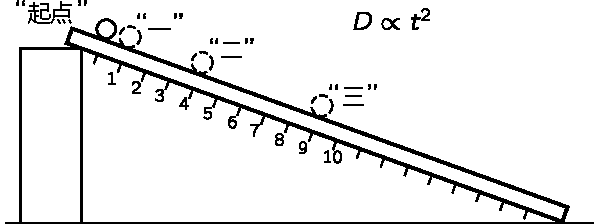
\includegraphics[width=0.35\textwidth]{Chapter5/一个小球沿着斜面滚下}
    \caption{一个小球沿着斜面滚下}
    \label{figure:一个小球沿着斜面滚下}
\end{wrapfigure}

当小球沿着轨道滚下时(图5.1),我们可以数自己的脉搏:“一…二…三…四…五…六…七…八…。”我们请一个朋友于每数一次就在小球所到达的位置上做一个小记号;然后就可以测量小球从被释放的位置开始在1个、2个或3个等等相等时间间隔内所经过的\uwave{距离}。伽利略用下面这种方法来表述\uwave{他的}观察结果:如果从小球释放的时刻算起,它的位置是在1,2,3,4,……单位时间记下的,那么这些记号离开起点的距离就正比于数1,4,9,16,……。今天我们就会这样说:距离与时间的平方成正比:
\begin{equation*}
D\propto t^2.
\end{equation*}

\uwave{运动}的研究对所有物理部门是一件基本的事,它所讨论的问题是何处与何时?


\section{时间}

让我们先来考察一下何谓\uwave{时间}。时间究竟是什么?假如我们能够找到时间的一个确切的定义那该是多好。在韦伯斯特辞典里把“一段时间(a time)”定义为“一个时期(a period)”,又把后者定义为“一段时间”。这种定义看来并不十分有用。或许我们应该说:“时间就是不发生其他事情时所发生的事。”然而这也未必使我们的理解深入。事实上(就字典的含义来说) 时间很可能是我们不能定义的事物之一。面对这个事实也许并没有什么不好。我们干脆说时间就是我们所知道的那回事:它就是我们等了多久!

不管怎样,重要的不在于我们是如何来\uwave{定义}时间,而在于我们如何来测量它 测量时间的一种方法是利用某种能以有规则的方式一再发生的事情,即某种能\uwave{周期性}发生的事情。例如,一个昼夜。昼夜似乎是一再重复出现的。然而你思索一下,也许就会问:“昼夜是否系真正周期性重复的?它们是否有规则地变化着?每一天是否都同样长?”人们肯定会有这种印象,夏天的日子比冬天的日子长。当然,在人们感到非常无聊的时候,总觉得冬天的有些日子长得可怕。你们一定会听到过有人这么说:“哎呀,这是多么长的一天!”

但是\uwave{就平均而言},日子确实大致一样长。我们有没有什么方法来检验日子——不论从一天到下一天,或者至少就其平均而论——长短相同与否?一个办法是把它同某种别的周期性现象作比较,我们来看怎样能用一个沙漏来做这种比较。如果我们让某个人昼夜站在它的旁边,每当最后一粒沙掉下之后,他就把沙漏倒转来,这样,我们用沙漏就能“创造”一个周期性的事件。

于是,我们就能计算从每天早上到下一天早上倒转沙漏的次数,这一次我们大概会发现每一“天”的“小时”数(即倒转沙漏的次数)并不相同。这样,我们就会猜疑太阳或者沙漏,或者怀疑这二者。在加以思索之后,我们或许会想到要计算从这个中午到下一个中午的“小时”数。(在这里中午的定义并不是12:00,而是指太阳在其最高点的时刻。)这一次我们将会发现,每一天的小时数都是相同的。

现在我们比较有把握认为“小时”和“昼夜”具有一种有规则的周期性,也就是说它们划分出相继的等时间间隔,虽然我们没有\uwave{证明}它们中不论那一个“确实”是周期性的。或许有人会问:是否会有某个万能者在夜间使沙漏中的流动变慢,而在白天又把它加快?我们的实验当然无法对这类问题做出回答,我们所能说的,只是发现一种事物的规则性与另一种事物的规则性相吻合而已。我们只能说把时间的\uwave{定义}建立在某种明显是周期性的事件的重复性上。


\section{短的时间}

现在我们要指出,在检验昼夜的重复性这个过程中我们获得了一个重要的副产品。这就是找到了一种比较精确地测量一天的\uwave{几分之一}的方法。亦即我们找到了一种用较小的间隔来计点时间的方法。能不能把这种过程再往前发展,从而学会测量甚至更小的时间间隔呢?

伽利略断定,只要一个摆的摆幅始终很小,那么它将总以相等的时间间隔来回摆动。如果做这样一个实验,对摆在一“小时”内的摆动次数进行比较,那么这个实验就会表明,情况确实如此。我们用这个方法可划分出一个小时的\uwave{几分之一}。假如我们利用一个机械装置计点摆动次数,并且保持摆动进行下去,那么就得到了我们祖父一代所用的那种摆钟。

让我们约定,如果我们的摆一小时内振动3600次(并且如果一天有24个这样的小时),那么我们就称每一摆动的时间为1“秒”。这样,就把原来的时间单位分成大约$ 10^5 $个部分。我们可以应用同样的原理把秒分成更加小的间隔。你们可以理解,制造一个能够走得任意快的机械摆是不现实的,但是我们现在能够制造一种称为振荡器的\uwave{电学摆}。这种电学摆能提供周期很短的摆动。在这种电子振荡器中,是电在来回振动,其方式与摆锤的摆动方式相类似。

我们可以制造一系列这种电子振荡器,每一个的周期要比前一个减小10倍。每一个振荡器可用前一个较慢的振荡器这样来“定标”,即数出较慢的振荡器振动一次时它所振动的次数。当我们的钟的振动周期小于一秒的几分之一时,如果没有某种辅助装置以扩展我们的观察能力,那就无从计点振动的次数。这种装置之一是电子示波器,它的作用就像一种供短的时间用的“显微镜”。这个装置在荧光屏上画出一幅电流(或电压)对时间的图像。将示波器依次与我们的系列中相继的两个振荡器相连,它就先显示出一个振荡器中的电流图像,然后显示出另一个振荡器中的电流图像,从而得到如图5.2所示的两幅图像。这样,我们就很容易测出较快的振荡器在较慢的振荡器的一个周期中振动的次数。

\begin{figure}
    \centering
    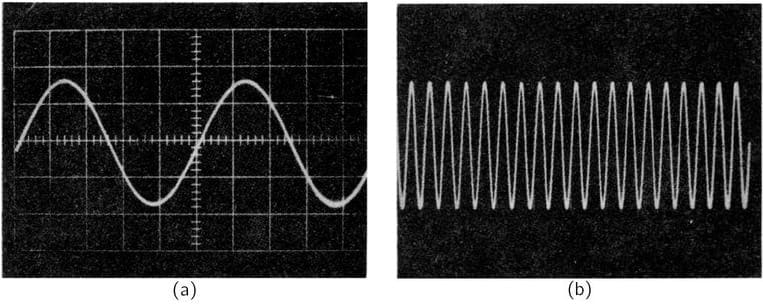
\includegraphics[width=0.8\textwidth]{Chapter5/示波器屏上的两个图象}
    \caption{\footnotesize 示波器屏上的两个图象。在(a)中,示波器与一个振荡器相连接;在(b)中,它与另一个其周期只有前者十分之一的振荡器相连接。}
    \label{figure:示波器屏上的两个图象}
\end{figure}

利用现代电子技术,已经制造出周期短到大约$ 10^{-12} $秒的振荡器,并且可以按照前面描述的那种比较方法用我们的标准时间单位——秒来予以定标。近年来,随着“激光器”或光放大器的发明和完善,已能制造周期甚至比$ 10^{-12} $秒更短的振荡器了,但是还不能用上述那些方法来予以定标,虽然毫无疑问,这在不久期间一定能够做到。

比$ 10^{-12} $秒还短的时间已经测量出来,但用的是另一种测量技术。事实上,这里所用的是“时间”的另一种\uwave{定义}。一个方法是观察发生在运动物体上的两个事件之间的\uwave{距离}。例如,假定有一辆行驶的汽车把它的车灯先开亮,然后再关掉。如果我们知道车灯开、关的\uwave{地点},以及车速,那么我们就能求出灯开的时间有多长。这段时间就是灯开时所通过的距离除以汽车的车速。

近几年来,正是这种技术被用来测量$\pi^0$介子的寿命。$\pi^0$介子在感光乳剂中产生并在其中留下微细的踪迹,用显微镜观察这些踪迹时,人们就可看到,平均而言一个$\pi^0$介子(认为它以近于光速的某个速度运动)在蜕变之前大约走过了$ 10^{-7} $米的距离,所以它的寿命总共只有大约$ 10^{-16} $秒。但是必须着重指出,这里我们用了一个与前稍有不同的“时间”的定义。然而,只要在我们的理解方面不出现任何不协调的地方,那么我们就觉得有充分的信心认为这些定义是足够等效的。

在把我们的技术——而且如有必要也把我们的定义——进一步加以扩展之后,就能推断更快物理事件的持续时间,我们可以谈论原子核振动的周期,以及第二章中提到过的那种新发现的奇异共振态(粒子)的寿命。它们的全部寿命只不过占$ 10^{-24} $秒的时间,大致相当于光(它以我们已知的最快速度运动)通过氢原子核(这个已知的最小物体)所花的时间。

那么,再短的时间呢?是不是还存在尺度更小的“时间”?如果我们不能够测量——或者甚至合理地去设想——某些发生在更短时间内的事情,那么要谈论更短的时间是否还有任何意义?可能没有意义。这是一些尚未解决的、但你们会提出的、而且也许在今后二十或三十年内才能回答的问题。


\section{长的时间}

我们现在来考虑比一昼夜还长的时间。要测量较长的时间很容易,我们只要数一数有几天就是——只要旁边有人在做这种计数的工作。首先我们发现,自然界里存在着另一个周期性,即年,一年大约等于365天。我们还发现,自然界有时也为我们提供了计算年的一些东西,例如树木的年轮或河流底部的沉积物。在某些情况下,我们就能利用这些自然界的时间标记来确定从发生某种事件以来所经历的时间。

当我们不能用计算年的方法来测量更长的时间时,那就必须寻找其他的测量方法。最成功的方法之一是把放射性材料作为一只“钟”来使用。在这种情况下,并不出现像昼夜或摆那样周期性的事件,但是有一种新的“规则性”。我们发现,某种材料的样品,当它的年龄每增加一相同的数值时,它的放射性就减少一相同的\uwave{分数}。假如我们画一张图来表示所观察到的放射性作为时间(比方以天来计算)的函数,那么我们就得到如图5.3所示的一条曲线。我们看到,如果放射性在$ T $天内减少到一半(称为“半衰期”),那么它在另一个$ T $天内就减少到四分之一等等。在任一时间间隔$ t $内共包含了$ t/T $个半衰期,而在这段时间$ t $后尚剩下的部分则是$ (\tfrac{1}{2})^{t/T} $。

\begin{table}[!ht]
    \centering
    \caption{时间}
    \setlength{\tabcolsep}{7mm}{
    \begin{tabular}{|cc|cc|}
    \hline
        年 & 秒 & ~ & 等效平均寿命物质 \\ \hline
        ~ & ~ & ?????? & ~ \\ \hline
        ~ & $10^{18}$ & 宇宙的年龄 & $U^{238}$ \\ \hline
        $10^9$ & ~ & 地球的年龄 & ~ \\ \hline
        ~ & $10^{15}$ & ~ & ~ \\ \hline
        $10^6$ & ~ & 最早的人 & ~ \\ \hline
        ~ & $10^{12}$ & 金字塔的年龄 & ~ \\ \hline
        ~ & ~ & ~ & $Ra^{226}$ \\ \hline
        $10^3$ & ~ & 美国的历史 & ~ \\ \hline
        ~ & $10^9$ & 一个人的寿命 & $H^3$ \\ \hline
        ~ & $10^6$ & 一天 & ~ \\ \hline
        ~ & $10^3$ & 光从太阳射到地球 & 中子 \\ \hline
        ~ & 1 & 一次心跳 & ~ \\ \hline
        ~ & $10^{-3}$ & 声波的周期 & ~ \\ \hline
        ~ & $10^{-6}$ & 无线电波的周期 & $\mu$介子 \\ \hline
        ~ & ~ & ~ & $\pi^{\pm}$介子 \\ \hline
        ~ & $10^{-9}$ & 光通过1ft的距离 & ~ \\ \hline
        ~ & $10^{-12}$ & 分子转动的周期 & ~ \\ \hline
        ~ & $10^{-15}$ & 原子振动的周期 & ~ \\ \hline
        ~ & ~ & ~ & $\pi^0$介子 \\ \hline
        ~ & $10^{-18}$ & 光经过一个原子 & ~ \\ \hline
        ~ & $10^{-21}$ & 核振动的周期 & ~ \\ \hline
        ~ & $10^{-24}$ & 光经过一个原子核 & 奇异粒子 \\ \hline
        ~ & ~ & ????? & ~ \\ \hline
    \end{tabular}}
\end{table}

如果我们知道一块材料比如说一块木料,在它形成时其中含有数量为$ A $的放射性物质,而用直接测量我们发现它此刻的量为$ B $,那么只要解方程
\begin{equation*}
(\frac{1}{2})^{t/T}=\frac{B}{A}
\end{equation*}
就能计算这一物体的年龄$ t $。

\begin{wrapfigure}{r}{0.45\textwidth}
    \centering
    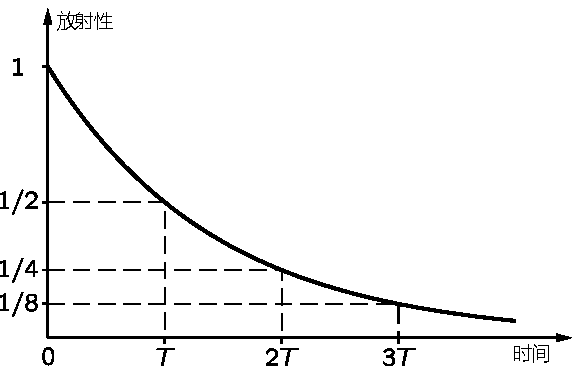
\includegraphics[width=0.35\textwidth]{Chapter5/放射性随时间而减少}
    \caption{\footnotesize 放射性随时间而减少。在每一个“半衰期”$ T $中,放射性都减少一半}
    \label{figure:放射性随时间而减少}
\end{wrapfigure}
幸运的是,在某些情况中,我们可以知道物体在形成时它所包含的放射性总量。比如说我们知道空气中的二氧化碳含有某一确定小量的放射性碳同位素C$ ^{14} $(它由于宇宙线作用而连续不断地得到补充),如果我们测量一个物体的碳的总含量,并且知道这个总含量的某一分数原来是放射性的C$ ^{14} $,那么,我们就知道上述公式中所要用到的那个开始时的总含量$ A $ 。碳14的半衰期是5000年,通过仔细的测量我们测出经20个左右的半衰期后所余留下来的数量。因此,我们就能够确定生长于100,000年以前那样古老的有机体的年代。

我们很想知道,并且认为也能知道比之更老的那些事物的寿命。许多有关这方面的知识,我们是通过测量具有不同半衰期的其他放射性同位素而得到的。如果我们用一种半衰期更长的同位素来进行测量,那么就能测得更长的时间。例如,铀有一种同位索,它的半衰期大约为$ 10^9 $年,所以如果有一种物质在它$ 10^9 $年前形成时就含有这种铀,那么今天这种铀就只剩下一半。当铀蜕变时,它变成了铅。设想有一块岩石,它是在很久以前通过某种化学过程形成的。铅由于具有与铀不同的化学性质,它将出现在岩石的一个部分中,而铀则出现在岩石的另一部分中。铀和铅将互相分开。如果我们今天来考察那块岩石将发现在那种应该只有铀存在的地方,现在有某一分数的铀和某一分数的铅,通过对这两个分数的比较;我们就能说出百分之几的铀已消失并且变成了铅。利用这个方法,有些岩石的年龄被测定为几十亿年。这个方法的一个推广便是不用特定的岩石,而是着眼于海洋中的铀和铅,并且对整个地球取其平均值。用这个推广了的方法(在过去几年中)曾测得地球本身的年龄为大约55亿年。

人们发现,地球的年龄与掉到地球上的陨石(也是用铀方法测定的)的年龄是相同的,这是一件令人鼓舞的事情。看来,地球是由漂游在太空中的岩石形成的,而陨石很可能就是遗留下来的那些物质的残片。在50亿年前的某个时候,宇宙开始形成。现在人们认为,至少我们这部分宇宙起源于大约100或120亿年之前。我们不知道在此之前发生过什么事情。事实上我们又可以提出来问:这个问题是否有任何意义?更早的时间是否有任何意义?


\section{时间的单位和标准}

我们在前面实际上已表明了,如果从时间的某个标准单位,比如一天或一秒出发,并把所有其他的时间表示为这个单位的倍数或分数,那么将十分方便。然而,我们将用那个单位作为我们的时间基本标准呢?是否用人的脉搏跳动?如果我们比较各人的脉搏,那就会发现它们之间似乎差别很大。如果比较两只钟,则发现它们的变化不那么大。于是你们会说:好,就让我们采用钟吧!但是用谁的钟呢?有个故事讲到一个瑞士男孩,他想使他所在的镇上所有的钟在正午时刻都同时敲响,所以他就跑来跑去,穿家过院,想使人人相信这样做的好处。每个人都想,如果他的钟在正午敲响时,其他钟也全都敲响的话,这该是一个多好的主意呀!然而要决定谁的钟应该取作标准,这倒是一件难事。幸运的是,我们大家都同意用一只钟,即地球。在很长一段时间里,人们把地球的自转周期当作时间的基本标准。但是当测量越来越变得精确的时候,人们发现,用最好的钟来进行测量,地球的转动也不是严格周期性的。我们有理由相信,这些“最好”的钟是精确的,因为它们彼此之间是相符的。由于种种理由,我们现在认为,有些天要比另一些天长,有些天要比另一些天短,平均而论,地球的自转周期是随着一个世纪一个世纪的过去而变长了一点的。

直到晚近以前,我们还没有找到任何一个比地球的周期好得多的标准,所以把所有的钟同一天的长度联系了起来,而把一秒规定为一个平均日的$  1/86400$。最近我们对自然界中某些振荡器获得了一些经验。我们现在相信,这些振荡器可以当作比地球更稳定的时间参考物。而且,它们也是基于一个大家都能采用的自然现象。这就是所谓的“原子钟”。它的基本的内在周期,就是原子振动的周期,这种振动对于温度或任何其他外界影响都不十分敏感。原子钟能使时间的精确度达到$ 10^9 $分之一,或者比之更高。在过去二年中,哈佛大学的拉姆齐(N.Ramsay)教授研制了一种改进的原子钟,它是依靠氢原子的振动而工作的。拉姆齐认为,这种钟比其他原子钟精确100倍。现在他正在对之作测量,这些测量将表明他的说法是否正确。

既然现在有可能制作远比天文时间精确的钟,那么我们可以预期,科学家们不久就会一致同意采用许多原子标准钟中的一种来定义时间单位\footnote{1967年的第十三届国际计量大会已通过决议将时间单位“秒”的定义改为:“一秒等于铯133原子基态的两个超精细能级之间跃迁的辐射周期的9,192,631,770倍。”——译者注。}



\section{长的距离}
现在我们转到\uwave{距离}的问题上来。事物有多远,或者有多大?人们都知道测量距离的方法是选用一种长度单位再加上计数,例如可以用尺或拇指边量边数。那么怎样来量比较小的东西呢?怎样把距离分小呢?这与我们将时间分小一样,我们同样取一个较小的单位,然后数出这个单位组合成一个较长单位时所需的数目。这样我们就能测量越来越小的长度。

\begin{wrapfigure}{r}{0.45\textwidth}
    \centering
    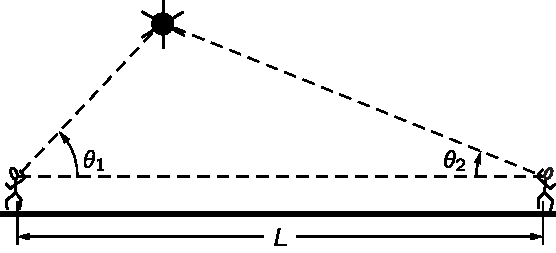
\includegraphics[width=0.35\textwidth]{Chapter5/用三角法测定人造卫星的高度}
    \caption{用三角法测定人造卫星的高度}
    \label{figure:用三角法测定人造卫星的高度}
\end{wrapfigure}
但是我们并不总是把距离理解为用米尺量。得的结果。仅仅用一根米尺是难以测量两个山顶之间的水平距离的。我们曾经凭经验发现可以用另一种方式来测量距离:即用三角法。虽然这意味着我们实际上对距离用了一个不同的定义,但当它们可以一起应用时,就应是彼此相一致。空间或多或少有点像欧几里得所设想的那个样子,所以距离的这两种定义是一致的。既然它们在地球上相一致,那就使我们充满信心可用三角法来测量更大的距离。例如,我们当时曾用三角法测定了第一颗人造卫星的高度(图5.4)。我们测得的高度约有$ 5\times 10^5$米。如果测量得更仔细一点,则用同样的方法可以测出地球到月球的距离;安放在地球上两个不同地点的两个望远镜,将会告诉我们所需要的两个角度。用这种方法我们求得月球离我们有$ 4 \times 10^8 $米远。

对于太阳,我们不能这样做,或者至少到现在没有人能够这样做。由于我们不能相当精确地对准太阳上一个特定的点,从而不能精确地测出两个角度,所以无法测出到太阳的距离。然而如何来测量这个距离呢?我们必须将三角法这个观念加以引伸。我们可以通过天文观察方法来测量所有行星出现的位置之间的相对距离,从而得到一幅有关太阳系的图像,能显示每个行星间的相对距离,但都不是绝对距离。因此需要测出一个\uwave{绝对}距离,而这种绝对测量已用几种方法得到,其中直到最近以前还认为最精确的一个是测出地球到爱神星的距离。爱神星是一个时常靠近地球的小行星。如果对这个小天体应用三角法,就能得到一个所需要的比例尺度。由于知道了其他天体的相对距离,我们就能说出它们之间的绝对距离,例如地球到太阳,或地球到冥王星的绝对距离。

\begin{figure}[htbp]
    \centering
    \begin{minipage}[t]{0.4\textwidth}
        \centering
        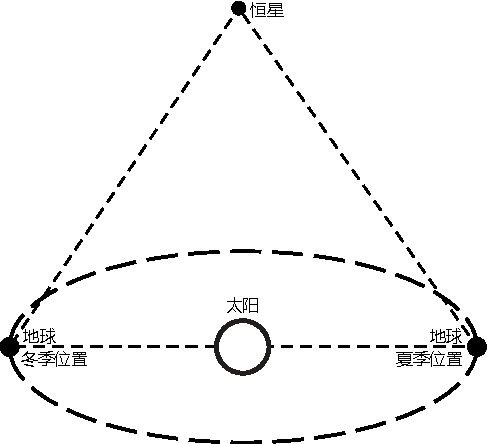
\includegraphics[width=5cm]{Chapter5/三角法测量恒星距离}
        \caption{\footnotesize 利用地球轨道的直径作为基线,可以用三角法测量靠近地球的恒星的距离}
    \end{minipage}
    \begin{minipage}[t]{0.4\textwidth}
        \centering
        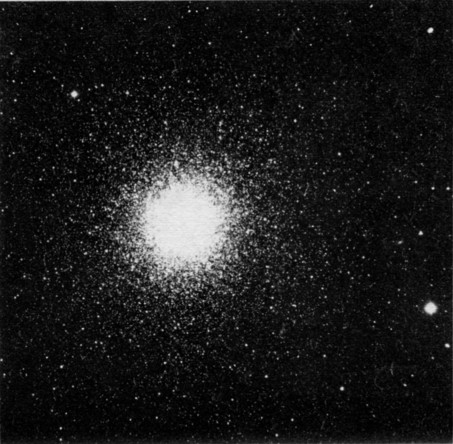
\includegraphics[width=5cm]{Chapter5/靠近我们银河系中心的一个星团}    
        \caption{\footnotesize 靠近我们银河系中心的一个星团,其中各恒星与地球的距离为30,000光年,或约$ 3\times 10^{20} $米}
    \end{minipage}
\end{figure}

去年,我们在有关太阳系的比例尺度的了解上获得了巨大的进展。喷气推进实验室用直接的雷达观察非常精确地测定了地球到金星的距离。当然,这只是另外一种由推测而得到的距离。我们说,我们知道光传播的速度(因而这也是雷达波传播的速度),并且假定,在地球与金星之间无论何处这个速度都相同。那么,在发射无线电波并测得电波返回的时间,我们就能从\uwave{时间}来推测\uwave{距离}。这确实是距离测量的另一种定义。

可是我们如何来测量一个更遥远的恒星的距离呢?幸运的是,我们可以回到三角法上来,因为地球绕太阳公转,而这种转动就为测量太阳系外的恒星距离提供了一条基线。假如我们在夏天和冬天用望远镜对准一颗恒星,那么我们可以期望能足够精确地测出这两个角度,从而能测出地球到恒星的距离。

如果恒星离得太远而不能应用三角法时又怎么办?天文学家总是在发明测量距离的新方法。例如,他们发现,从恒星的颜色可以估计它的大小和亮度。他们测定了许多靠近地球的恒星——这些恒星的距离已用三角法测得——的颜色和内在亮度,并且发现在恒星颜色和内在亮度(在大多数情况中)之间存在着一个平滑的关系,如图5.5所示。如果现在测出了一个遥远恒星的颜色,那就可以用颜色—亮度关系来确定这个星体的内在亮度,在测量了我们地球上看来这颗恒星有多亮(或许应该说有多\uwave{暗})之后,我们就可以计算它有多远(对于一个给定的内在亮度,其表观亮度是随距离的平方而减小的)。对称为球状星团的一群恒星作测量后,所得的结果很好地证实了这种星际距离测量方法的正确性。图5.6是这样一群恒星的一张照片。只要看一下照片,人们就会相信这些恒星都聚集在一起。用颜色—亮度关系这个测量距离的方法得到了同样的结果,

\begin{figure}[htbp]
    \centering
    \begin{minipage}[t]{0.4\textwidth}
        \centering
        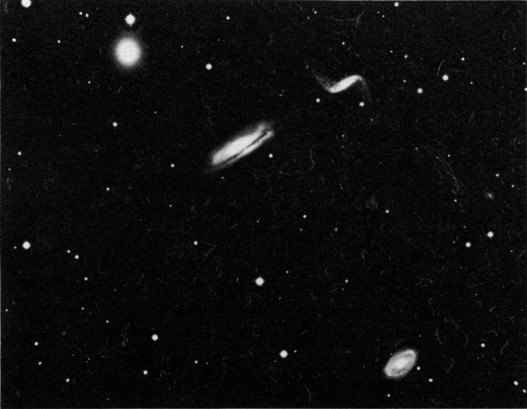
\includegraphics[width=6cm]{Chapter5/和我们银河系一样的一个螺旋银河系}
        \caption{\footnotesize 和我们银河系一样的一个螺旋银河系,假定它的直径与我们银河系相近,那么我们从它的表观大小就能算出它的距离。它离地球约3000万光年(即$ 3\times 10^{23} $米)}
    \end{minipage}
    \begin{minipage}[t]{0.4\textwidth}
        \centering
        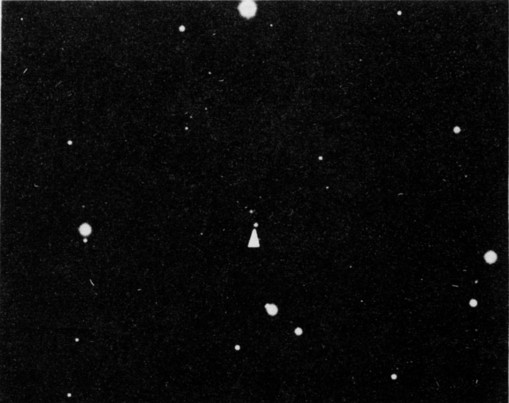
\includegraphics[width=6cm]{Chapter5/牧夫座中的3c295}    
        \caption{\footnotesize 最现代化的200英寸望远镜拍摄的最远天体——牧夫座中的3C295(用箭头标出)}
    \end{minipage}
\end{figure}
对许多球状星团进行研究之后使我们得到另一些重要信息。人们发现,在天空的某一部分有许多这样的星团高度集中在一起,而且其中大部分离地球的距离大致相同。把这个信息和其他证据结合起来,就能断定,星团的这个集中处就是我们所在银河系的中心。于是我们就知道到银河系中心的距离——大约为$ 10^{20} $米。

知道了我们自己所在银河系的大小,我们就有了一把测量更大距离——也就是到其他银河系的距离——的钥匙。图5.7是一副形状与我们的银河系颇为相同的一个银河系的照片。它的大小可能也和我们的相近。(另外的一个证据支持了这种想法,即所有银河系都有相近的大小。)假如确实如此,那我们就能说出它的距离,我们测量它在天空中的张角,又知道了它的直径,于是就能算出它的距离——这又是三角法!

新近用巨大的帕洛马望远镜获得了极其遥远的一些银河系的照片,图5.8是其中的一张。现在人们认为,这样的一些银河系大约处在从地球到我们宇宙界限——$ 10^{26} $米处——一半的地方。$ 10^{26} $米是我们能想象的最大最大距离!


\section{短的距离}
现在我们考虑一下小的距离。把一米分小是很容易的,把一米划分成一千个相等的间隔并没有多大困难。用相似的方法(利用一架好的显微镜),我们能够把1毫米分成一千等分,构成微米(一米的百万分之一)这样的尺度,但这要稍微困难一些。要继续分成更小的尺度则很困难,因为我们“看不见”一个比可见光波长(大约$ 5\times 10^{-7} $还要小的物体。

\begin{wrapfigure}{l}{0.4\textwidth}
    \centering
    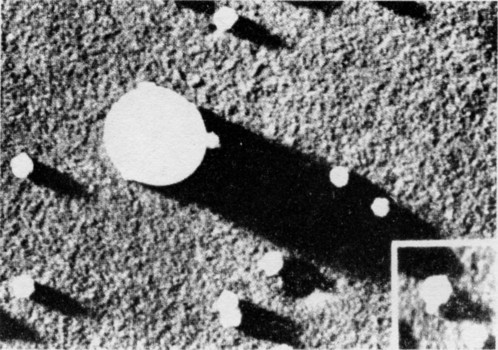
\includegraphics[width=0.35\textwidth]{Chapter5/某些病毒分子的电子显微镜图}
    \caption{\footnotesize 某些病毒分子的电子显微镜图。“大的”球是为定标用的,且已知其直径为$ 2\times 10^{-7} $米(2000 Å)}
    \label{figure:某些病毒分子的电子显微镜图}
\end{wrapfigure}
然而我们毋须停止在我们看得见的东西上,依靠电子显微镜,我们能用拍照方法来对更小的尺度(比方说一直到$ 10^{-8} $米)继续这个划分过程(图5.9)。

用间接的测量,即用一种显微镜规模的三角法,我们能对越来越小的尺度继续进行测量。首先我们从观察波长短的光(X射线)如何在间隔为已知的标记所组成的图样上被反射的情况,确定光振动的波长。然后从同样的光在一块晶体上所散射的图样,我们就能确定原子在晶体中的相对位置,所得结果与化学方法确定的原子间距离相符合。用这种方法我们发现原子的直径约为$10^{-10}$米。

典型的原子大小约为$10^{-10}$米,而原子核的大小为$10^{-15}$米,其间相差$10^5$倍!可见原子与原子核之间在物理大小上存在一个很大的“空隙”。对原子核的大小来说,用另一种测量方法比较方便。我们测量的是它的\uwave{表观面积}$\sigma$,称之为有效截面。如果要知道半径,则可从$\sigma=\pi r^2$求得,因为原子核是近似球形的。

核的截面可以这样来测量,使一束高能粒子通过某种材料的一块薄板,然后观察没有通过薄板的粒子数,这些高能粒子通常会穿过薄薄的电子云,而只有当它们碰上了质量集中的原子核时,才会被阻止或者被偏转。假设我们有一块1厘米厚的材料,其中大约有$10^8$个原子核。但原子核如此之小,以致一个核恰好位于另一个核的背后的机会是很小的。我们可以\uwave{设想},这种情况的一个高度放大的图像——沿着粒子束看去时——犹如图5.10所示。

\begin{wrapfigure}{r}{0.4\textwidth}
    \centering
    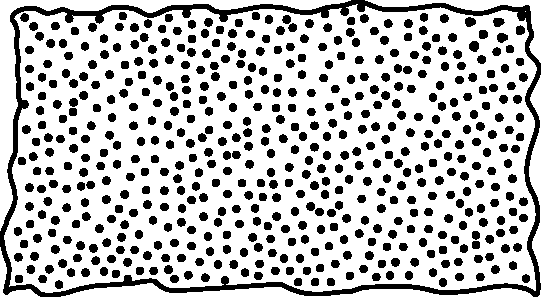
\includegraphics[width=0.35\textwidth]{Chapter5/一块厚1厘米的碳设想的图像}
    \caption{\footnotesize 在只观察核的时候,通过一块厚1厘米的碳所见到的那个设想的图像}
    \label{figure:一块厚1厘米的碳设想的图像}
\end{wrapfigure}
一个很小的粒子在通过物质时能打在一个核上的概率,正好等于其中所有核的剖面所占的总面积除以这幅图上的总面积。假定我们知道在这块板的面积$A$中有$N$个原子(当然,每个原子只有一个核),那么被这些核所“覆盖”的面积和总面积之比就等于$N \sigma / A$。现在设粒子束中射到薄板的粒子数为$n_1$,从薄板另一边射出的粒子数为$n_2$。这样,\uwave{没有} 通过薄板的粒子数和射出的粒子数之比为$(n_1-n_2)/n_1$,它们应该正好等于被覆盖面积和总面积之比。于是从等式\footnote{只有当核所覆盖的面积是总面积的一个很小分数,即$(n_1-n_2)/n_1$远比1小时,这一等式才正确。否则我们必须对有些核将部分地为其前面的核所挡住这样的情况进行校正。}
\begin{equation*}
\pi r^2=\sigma=\frac{A}{N}\,
(\frac{n_1-n_2}{n_1})
\end{equation*}
就能获得核的半径。

从这样一种实验我们得出核的半径大约为$10^{-15}$米的一到六倍。$10^{-15}$米这个长度单位称为\uwave{费米},以纪念著名的物理学家费米(1901~1958)。

\begin{table}[!ht]
    \centering
    \setlength{\tabcolsep}{13mm}{
    \begin{tabular}{|cc|c|}
    \hline
        光年 & 米 & ~ \\ \hline
        ~ & $10^{27}$ & ?????? \\ \hline
        $10^9$ & ~ & 宇宙的边缘 \\ \hline
        ~ & $10^{24}$ & ~ \\ \hline
        $10^6$ & ~ & 到最邻近的银河系 \\ \hline
        ~ & $10^{21}$ & ~ \\ \hline
        $10^3$ & ~ & 到银河系中心 \\ \hline
        ~ & $10^{18}$ & ~ \\ \hline
        1 & ~ & 到最近的恒星 \\ \hline
        ~ & $10^{15}$ & ~ \\ \hline
        ~ & ~ & 冥王星的轨道半径 \\ \hline
        ~ & $10^{12}$ & ~ \\ \hline
        ~ & ~ & 到太阳 \\ \hline
        ~ & $10^{9}$ & ~ \\ \hline
        ~ & ~ & 到月球 \\ \hline
        ~ & $10^{6}$ & ~ \\ \hline
        ~ & ~ & 人造卫星高度 \\ \hline
        ~ & $10^{3}$ & ~ \\ \hline
        ~ & ~ & 电视塔高度 \\ \hline
        ~ & $1$ & 一个孩子的高度 \\ \hline
        ~ & $10^{-3}$ & ~ \\ \hline
        ~ & ~ & 一粒盐 \\ \hline
        ~ & $10^{-6}$ & ~ \\ \hline
        ~ & ~ & 病毒 \\ \hline
        ~ & $10^{-9}$ & ~ \\ \hline
        ~ & ~ & 原子半径 \\ \hline
        ~ & $10^{-12}$ & ~ \\ \hline
        ~ & $10^{-15}$ & 原子核半径 \\ \hline
        ~ & ~ & ?????? \\ \hline
    \end{tabular}}
\end{table}

如果我们进到更小的距离,那么将会发生什么呢?能不能测量更小的距离?这样的问题现在还不可能回答。有人提出这种看法,认为迄今尚未解决的核力之谜,只有在对这样小的距离下的我们关于空间或测量的观念进行某些修正以后才能解开。

人们也许会想到,用某些自然长度来作为我们的长度单位——比如说地球的半径或者它的某一部分——倒是一个很好的意见。米之取作为单位只是出于这样的考虑,它被定义为地球半径的$(\pi/2)\times10^{-7}$倍。但是,用这种方法来规定长度单位,既不方便,也不很准确。很长时间以来国际上大家约定:一米的定义是保持在法国一个特殊实验室中的一根棒上两条刻线之间的距离。不久前人们认识到这个定义既未精确到足以使之有用,也不像人们所希望的那样稳定或普遍。近年来正在考虑采用一个新的定义,即选定一根光谱线,把大家一致同意的它的波长的(任意)倍数作为长度的单位。

距离测量和时间测量的结果有赖于观察者。两个作相互运动的观察者在测量看来似乎是同一个的事物时,将不会得到同样的距离和时间。距离和时间间隔随着测量时所用的坐标系(或“参考系”)不同而有不同的大小。我们将在后面的一章中详细地研究这个问题。

完全精密的距离测量或时间测量是为自然规律所不允许的。我们前面已经提到,在测量一个物体的位置时,误差至少要像
\begin{equation*}
\Delta x\geq\frac{\hbar}{2\Delta p},
\end{equation*}
那样之大,其中$\hbar$是一个称为“普朗克常数”的很小的量,而$\Delta p$是我们在测量物体的位置时,对它的动量(质量乘以速度)的知识上的误差。我们也曾提到,位置测量的不确定性是与粒子的波动本质有关的。

空间和时间的相对性意味着时间的测量也有一个实际由
\begin{equation*}
\Delta t\geq\frac{\hbar}{2\Delta E},
\end{equation*}
给出的最小误差,其中$\Delta E$是我们在测量一个过程的时间时,对它的能量的知识上的误差。如果我们要\uwave{更}精确地知道某个事件\uwave{何时}发生,那就只能对发生了什么知道得更少一点,因为我们对其所含能量的知识减少了。时间的不确定性也是与物质的波动本质有关的。


\chapter{概率}

\begin{quote}[J. C. 麦克斯韦]
我们这个世界的真正逻辑寓于概率的计算之中。
\end{quote}

\section{机会和可能性}

“机会”是日常生活中通常使用的一个词汇。无线电在播送明天的天气预报时可能会说:“明天下雨的机会是百分之六十。”你也许会说:“我能活上一百岁的机会是不大的。”科学家也使用机会这个词。一个地震学家可能会对这样的问题感兴趣:“明年在南加利福尼亚州发生某一级地震的机会有多大?”一个物理学家也许会提出这样的问题:“在下一个十秒钟内,某一特定盖革计数器将记录到20个计数的机会是多少?”一个政治家或国务活动家可能对下列问题感兴趣:“下一个十年内发生核战争的机会是多少?”同样,你也许会对从这一章中将学到一些的机会发生兴趣。

所谓\uwave{机会}指的是某种类似于猜测的事。为什么我们要猜测呢?希望作出判断而只掌握不完全的信息或不确定的知识时,我们就要进行猜测。我们要对这是些什么东西或者可能发生什么事情进行猜测。由于必须作出决定,我们常常要进行猜测。比如说,明天我是否要带上雨衣?我应设计一座能够防御哪种程度地震的新大厦?我是否要为自己建造一个放射性微粒掩蔽所?我是否要在国际谈判中改变自己的立场?我今天是否要去上课?

有时我们所以要进行猜测,是因为我们想用自己有限的知识来对某种情况说出尽可能多的东西。\textbf{事实上,任何一个判断本质上都是一种猜测。同样,任何物理理论都是一种猜测,其中有成功的,也有失败的}\footnote{这里只是简单提一下,实际上这句话蕴含了极深极丰富的哲学思想。}。概率论就是为进行较好猜测而产生的一种理论体系。应用概率的语言能使我们定量地谈论某些情况,而这些情况的变化可能很大,但确有某种一贯的平均行为。

让我们来研究向上抛掷硬币这件事。如果抛掷——以及硬币本身——都是“可靠”的,那么对任何一次特定的抛掷,我们无法预期能得到什么样的结果。然而我们可能会感到,在大量的抛掷中应该得到数目大致相等的正面和反面。我们说:“每次抛掷以正面落地的概率是0.5。”

我们只是为了对将来要做的那些观察而谈到概率的。所谓在一次观察中将得到一个特定结果的“概率”,就是指我们在大量重复这个观察时对其中出现该特定结果的最可能分数的估计。如果我们设想重复某种观察——比如看一下刚抛掷的硬币——$N$次,并且称$N_A$为我们对这些观察中最可能出现某一指定结果$A$——比如出现“正面”的数的\uwave{估计}。那么所谓观察到$A$的概率$P(A)$就是指:
\begin{equation}
\label{Eq:I:6:1}
P(A)=\frac{N_A}{N}.
\end{equation}

对我们这个定义,需要作几点注释。首先,只有当所发生的事件是某一\uwave{可重复}的观察的可能结果时,我们才能谈到发生某件事的概率。像“那所房子里出现一个幽灵的概率是多少?”这类问题有没有任何意义是不清楚的。

你可以争辩说,没有一种情况可以\uwave{不折不扣}地重复。这是对的。每一个不同的观察至少必须在不同的时间或者不同的地点进行。我们所能说的只是,对于我们想要达到的目的来说,凡是重复进行的观察应该看来似乎都是\uwave{等价的}。至少我们应当这样假定,每一次观察都在同样准备好的情况下进行,特别是在观察开始时都要带有同等程度的无知。(玩纸牌时,如果我们偷看一下对方的牌,那么我们对自己获胜的机会的估计就显然与偷看前不同!)

我们应当强调指出,式(6.1)中的$N$和$N_A$并\uwave{不}代表实际所作观察的次数。$N_A$是我们在$N$个\uwave{想像}的观察中\uwave{可能}得出结果$A$的观察的最佳\uwave{估计}。因此,概率有赖于我们的知识以及进行估计的能力。实际上有赖于我们的常识!幸运的是,常识对于许多事物都有一致程度的共同看法,所以不同的人将会作出同样的估计。然而,概率毋需是一些“绝对”的数字。既然它们与我们对事物的无知有关,那么如果我们所掌握的知识发生变化,它们也会变得不同。

你们也许已经注意到我们的概率定义中另一个相当“主观”的方面,我们把$N_A$说成是对最可能次数的一个估计……。可是这并不意味着我们\uwave{不折不扣}地期望能观察到$N_A$,而是期望能得到一个\uwave{靠近}$N_A$的数,而且数$N_A$比其邻近任何其他的数\uwave{更为可能}。比如说,我们抛掷一个硬币$30$次,那么我们可以预料,得到正面的数字不大可能正好是15,而很可能是某一靠近15的数,如12,13,14,15,16或17。然而,如果我们\uwave{必须}对之作出决择,那么我们就会决定,15次正面要比任何其他的数\uwave{更为可取}。我们将写成:P(正面)=0.5。

为什么我们选择15为一个比任何其他数更可取的数呢?我们一定会同自己以如下方式进行过争辩:如果在$N$次抛掷中得到正面的最可能次数为$N_H$,那么得到反面的最可能次数$N_T$就等于$N-N_H$。(这里我们作了这样的假定,即每次抛掷\uwave{不是}得到正面\uwave{便是}得到反面,不会得到“其他”结果! )但如果硬币是“可靠”的,它就既不偏向正面,也不偏向反面。除非有某些理由可以认为硬币(或者抛掷)是不可靠的,我们就必须认为正面与反面具有相等的可能性。所以必须使$N_T=N_H$。这样就得到$N_T=N_H=N/2$或者$P(H)=P(T)=0.5$。

我们可以把这一论证推广到任何一种情况;在这种情况下,可以观察到$m$个不同但又“相等”(即机会均等)的可能结果。如果通过观察能得到$m$个不同结果,而且又有理由相信,其中任何一个结果与别的任何结果同样可能,那么得到某一个\uwave{特定}结果$A$的概率就等于$P(A)=1/m$。

如果在一个不透明的盒子里有7个不同颜色的小球,我们“随便”(即不朝它看时)取出一个,那么得到某一种颜色的小球的概率是$1/7$。从已洗过的52张牌中“任意”抽出一张红桃10的概率是$1/52$。掷骰子而得到两个一点的概率是$1/36$。
\begin{center}
\makebox[200pt]{\hrulefill}
\end{center}

\begin{small}
从第五章中,我们用原子核的表观面积,或者称为“截面”来描写它的大小。这样做时,实际上我们就是在谈概率。当我们向一块薄的材料发射一个高能粒子时,它有一定机会直接穿过去,也有一定机会碰撞在一个原子核上。(既然原子核如此之小,以致我们无法\uwave{看到},我们就不可能直接瞄准,而必须“盲目射击”。)设在这块薄板中有$n$个原子,而每个原子的核具有截面积$\sigma$,那么被所有这些核所“遮盖”的总面积为$n\sigma$。在随机发射的很大数目$N$中,我们预期能击中\uwave{某些}核的数目$N_C$与$N$之比,犹如被遮盖的面积与薄板的总面积之比:
\begin{equation}
\label{Eq:I:6:2}
\frac{N_C}{N}=\frac{n\sigma}{A}.
\end{equation}
因此我们可以说,任何一个入射粒子在穿过薄板时将经受一次撞击的\uwave{概率}为
\begin{equation}
\label{Eq:I:6:3}
P_C=\frac{n}{A}\,\sigma,
\end{equation}
其中$n/A$是我们这块薄板中单位面积内的原子数。
\end{small}



\section{起伏}

\begin{wrapfigure}{r}{0.45\textwidth}
    \centering
    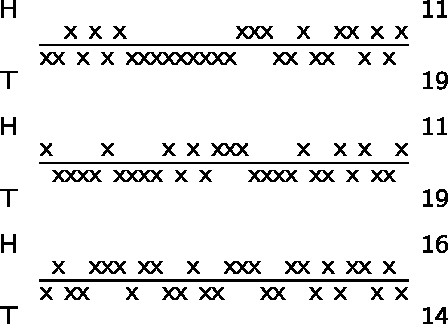
\includegraphics[width=0.35\textwidth]{Chapter6/三十次抛掷正面和反面的前后次序}
    \caption{\footnotesize 在每轮为30次抛掷的三轮游戏中所观察到的正面和反面的前后次序}
    \label{figure:三十次抛掷正面和反面的前后次序}
\end{wrapfigure}
我们现在想利用有关概率的概念来比较详细地考虑一下这样的一个问题:“如果我把一个硬币抛掷$N$次,那么预期真正会得到多少次的正面?”然而在回答这个问题之前,让我们先来看一下在这样一个“实验”中确实会发生什么情况。图6.1表示$N=30$的这样一个实验在前三"轮”中所得到的结果。

“正面”和“反面”的前后次序完全是按照它们得到时的次序排列的。第一轮得到11次正面;第二次也是11次;第三轮16次。在这三轮试验中,我们没有一回得到15次正面,是不是要对硬币发生怀疑呢?或者在这样一种游戏中,我们设想得到正面的最可能次数是15这一点错了呢?再做97轮实验,以便一共得到每回抛掷30次的实验100轮。实验的结果列在表6.1中:
\begin{table}[H]
\caption{\footnotesize 在抛掷一个硬币30次的逐轮试验中每轮所得正面的数目}
\centering
\medskip 
\begin{tabular}{p{20pt} p{20pt} p{20pt} p{20pt} p{20pt} p{20pt} p{20pt} p{20pt} p{20pt} p{20pt}}
\toprule
11 & 16 & 17 & 15 & 17 & 16 & 19 & 18 & 15 & 13     \\
11 & 17 & 17 & 12 & 20 & 23 & 11 & 16 & 17 & 14       \\
16 & 12 & 15 & 10 & 18 & 17 & 13 & 15 & 14 & 15     \\
16 & 12 & 11 & 22 & 12 & 20 & 12 & 15 & 16 & 12       \\
16 & 10 & 15 & 13 & 14 & 16 & 15 & 16 & 13 & 18       \\
14 & 14 & 13 & 16 & 15 & 19 & 21 & 14 & 12 & 15      \\
16 & 11 & 16 & 14 & 17 & 14 & 11 & 16 & 17 & 16      \\
19 & 15 & 14 & 12 & 18 & 15 & 14 & 21 & 11 & 16      \\
17 & 17 & 12 & 13 & 14 & 17 & 9  & 13 & 19 & 13    \\
14 & 12 & 15 & 17 & 14 & 10 & 17 & 17 & 12 & 11      \\    
\bottomrule        
\end{tabular}
\end{table}

\begin{wrapfigure}{r}{0.45\textwidth}
    \centering
    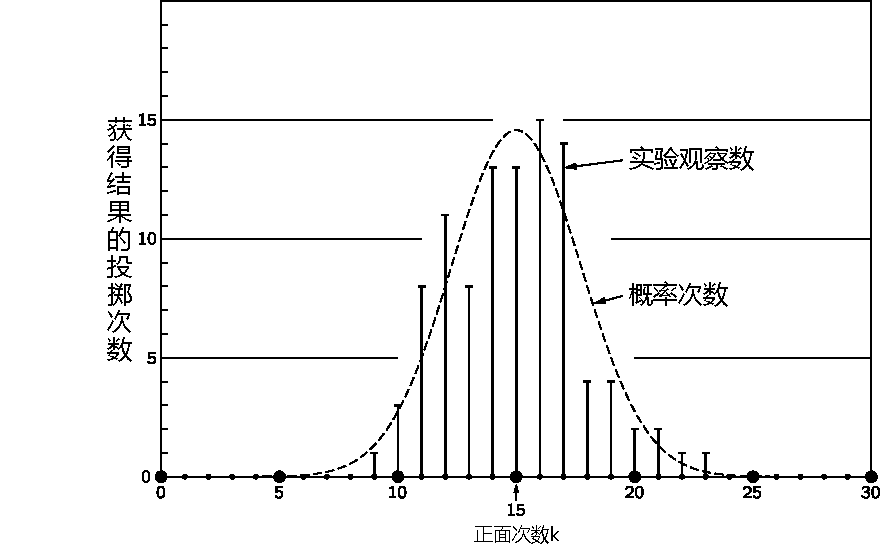
\includegraphics[width=0.43\textwidth]{Chapter6/30次抛掷的100轮游戏所得结果概况}
    \caption{\footnotesize 每轮30次抛掷的100轮游戏所得结果概况。垂直线表示记录到$k$次正面的各轮游戏的数目,虚线表示从概率计算求得的所期望记录到$k$次的游戏次数。}
    \label{figure:30次抛掷的100轮游戏所得结果概况}
\end{wrapfigure}
如果观察一下表6.1中所列出的各数,那么我们看到,大多数结果“靠近”15,而且位于12与18之间。如果我们为这些结果画一张\uwave{分布}图,那么就会对这些结果的细节有一个更好的理解。我们计算一下得到某一记录$k$的实验次数,并把这个数对每一个$k$作图,如图6.2所示,记录到15次正面的共13轮游戏,记录到14次正面的也是13轮。得到16的17次的,每一个都\uwave{大于}13轮,我们是否断定这里对正面有所偏袒?我们的" 最佳估计"2是否不够好?是不是我们现在不应该作出这个结论,即每轮30次抛掷的“最可能”记录实际上是16次正面?但是且慢!把所有各轮游戏加到一起,就总共抛掷了3000次,而获得正面的总数是1492次。可见出现正面的抛掷其比数是0.497,很接近而稍\uwave{小}于0.5。当然我们\uwave{不应}假定抛掷后得到正面的概率大于0.5!至于某\uwave{特定}的一组观察经常得到16次正面这个事实,是一种\uwave{起伏}现象,然而我们仍然预期\uwave{最可能}的正面数是15。

我们可以提出这样的一个问题:“在30次抛掷的游戏中将获得15,16,或任何其他次数正面的概率\uwave{是}多少?”我们已经说过,在抛掷一次的游戏中,得到\uwave{一次}正面的概率是0.5,得不到正面的概率也是0.5。在抛掷两次的游戏中,有\uwave{四种}可能的结果:即$HH, HT, TH, TT$。\footnote{这里H表示Head,即正面;T表示Tail,即反面。}既然这些结果中的每一个都是同样可能的,我们就推断出:(a)记录到两次正面的概率是$1/4$,(b)记录到一次正面的概率是$2/4$,(c)记录到零次的概率是$1/4$。这里有\uwave{两}种方式可以得到一次正面。但是得到两次或零次正面的方式各只有一种。

现在我们来研究抛掷3次的游戏,第三次抛掷同样可能得到一个正面或者一个反面。这里得到三次正面的方式只有一种:我们\uwave{必须}在前两次抛掷中得到两次正面,而后在最后一次中得到正面。可是这里有\uwave{三}种方式可以得到两次正面。在掷得两次正面(一种方式)后,我们可以掷出反面,或者在前两次抛掷中只掷出一次正面(两种方式)后,我们可以掷出一个正面。因此对于$3-H, 2-H, 1-H, 0-H$等记录,其同样可能的方式的数目分别为1,3,3,1。共有8种不同的可能结果。于是其概率分别为$1/8$,$3/8$,$3/8$,$1/8 $。

刚才的讨论可以用图6.3概括之。可以清楚地看到,对于更大数目的抛掷,应如何来把这个图画下去。图6.4是抛掷6次游戏的图解。

\begin{figure}[htbp]
    \centering
    \begin{minipage}[t]{0.4\textwidth}
        \centering
        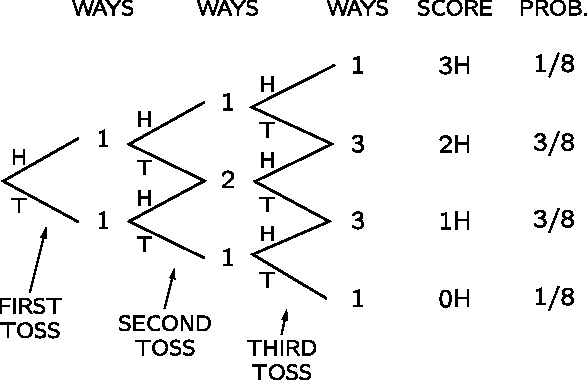
\includegraphics[width=5cm]{Chapter6/抛掷三次游戏的图解}
        \caption{\footnotesize 在抛掷三次的游戏中,能得到0,1,2,3次正面的方式数目的图解}
    \end{minipage}
    \begin{minipage}[t]{0.4\textwidth}
        \centering
        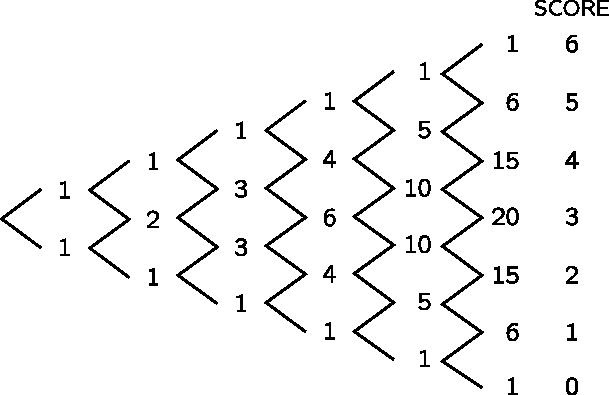
\includegraphics[width=5cm]{Chapter6/抛掷六次游戏的图解}    
        \caption{抛掷六次游戏的图解}
    \end{minipage}
\end{figure}

达到图中任何一点的所有“方式”的数目就是从起点开始到该点可以取的各种不同“途径”(即正面和反面相连的各种次序)的数目。最后一栏告诉我们掷得正面的总数。这样一种图表中出现的一组数称为\uwave{帕斯卡三角形}。这些数也称为\uwave{二项式系数},因为它们也出现在$(a+b)^n$的展开式中。如果我们称$n$为抛掷的次数,$k$为掷得正面的次数,那么图表中的数字通常用符号$\tbinom{n}{k}$来表示。顺便提一下,二项式系数也可以从式
\begin{equation}
\label{Eq:I:6:4}
\binom{n}{k}=\frac{n!}{k!(n-k)!},
\end{equation}
算出,其中$n!$称为“n阶乘”,表示连乘积$(n)(n-1)(n-2)\dotsm(3)(2)(1)$的意思。

我们现在打算根据式(6.1)来计算在$n$次抛掷中得到$k$次正面的概率$P(k,n)$。所有可能结果的总数是$2^n$(因为对每一抛掷有两个结果),得到$k$次正面的总共有$\tbinom{n}{k}$种,而每一种都是同样可能的,所以我们有
\begin{equation}
\label{Eq:I:6:5}
P(k,n)=\frac{\tbinom{n}{k}}{2^n}.
\end{equation}

既然$P(k,n)$是我们期望会得到$k$次正面的比数,那么在100轮游戏中,我们应预期共有$100\cdot P(k,n)$轮会出现$k$次正面。图6.2中虚线所经过的各点就是从$100 \cdot P(k,30)$计算出来的那些点子。我们可以看到,我们\uwave{预期}有14或15轮游戏会记录到15次正面,然而只有13轮游戏观察到这个记录,我们\uwave{预期}有13或14轮游戏会记录到16次正面,但是只有16轮游戏观察到这个记录。这样一种起伏情况实际上就是“这种游戏的组成部分”。

我们刚才用过的方法,可以应用于最一般的情况,也就是在单独一次观察中只能得出两种可能结果的情况。我们用$W$[表示“win”(赢)]和$L$[表示“lose”(输)]来表示这两种结果。在一般情况下,单独一个事件会得$W$或$L$的概率是毋需相等的。设$p$为得到结果$W$的概率,于是$q$——这个得到结果$L$的概率必然等于$(1-p)$。在一组$n$轮的试验中,得到$k$次结果为$W$的概率$P(k,n)$就等于
\begin{equation}
\label{Eq:I:6:6}
P(k,n)=\tbinom{n}{k}p^kq^{n-k}.
\end{equation}

这个概率函数称为\uwave{伯努利}或\uwave{二项式}概率。


\section{无规行走}

另一个有趣的问题也需要用到概率概念,这就是“无规行走”的问题。在最简单的形式下,我们可以想象这样一个“游戏”,其中“游戏者”从$x=0$的一点出发,要求他每“移动”一次\uwave{要末}朝前(向$+x$方向)走一步\uwave{要末}朝后(向$-x$方向)走一步。而朝前朝后必须\uwave{随机}决定,例如用抛掷硬币的方法。我们将怎样来描写这种行动的结果呢?在一般形式下,这个问题与气体中原子(或其他粒子)的运动,即布朗运动有关,也与测量中误差的组合有关。你们将会看到,无规行走问题与我们已讨论过的抛掷硬币问题密切有关。

首先,让我们看几个无规行走的例子。我们可以用行走者在$N$米中所经过的净距离$D_N$来表示他的进度。图6.5为无规行走者所走路径的三个例子。(这里我们用图6.1所示抛掷硬币所得的结果作为随机选择的移动取向。)

\begin{wrapfigure}{r}{0.45\textwidth}
    \centering
    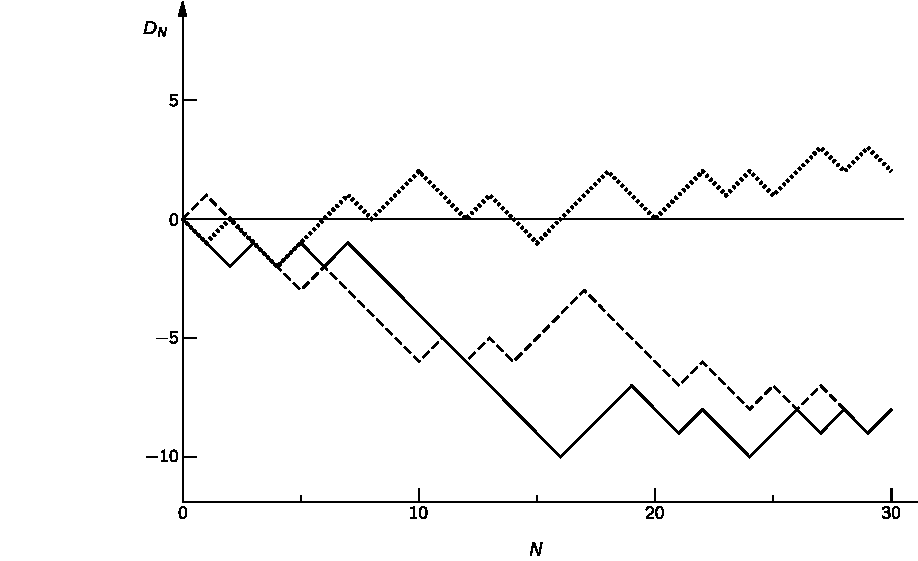
\includegraphics[width=0.35\textwidth]{Chapter6/无规行走取得的进度}
    \caption{\footnotesize 无规行走取得的进度。横座标$N$表示所走的步子总数;纵座标$D_N$表示离开起点的净距离}
    \label{figure:无规行走取得的进度}
\end{wrapfigure}

对于这样一种运动我们可以说些什么呢?首先我们也许会问:“平均而言他走了多远?”我们必定\uwave{预期}他的平均进度为零,因为他向前或向后走的可能性是均等的。然而我们似乎有这样的感觉,认为随着$N$的增加,他更可能偏离起点越来越远。因此我们也许要问,走过的用\uwave{绝对值}表示的平均距离是多少,也就是说$\abs{D}$的平均值是多少。可是在这里用另一个量度“进度”的方法更为方便,这就是用距离的平方$D^2$来表示,它无论对正的还是负的移动都为正,所以它是这种随机漫步的一个合理\uwave{量度}。

我们可以证明,$D_N^2$的预期值恰好是所走步子的数目$N$。所谓“期望值”,指的是可几值(也就是我们的最佳猜测),我们可以把它看作是对重复多次的一系列行走所\uwave{预期}的平均行为。我们用$\left <D_N^2 \right >$来表示这样一个预期值,并且也可以称它为“平均平方距离”。走一步后的$D^2$总是$+1$,所以当然$\left < D_1^2 \right >=1$。(所有的距离都将以一步为单位来量度。以后我们将不再写出距离的单位。)

当$N>1$时,预期值$D_N^2$可以从$D_{N-1}$求得。如果走了$(N-1)$步后,我们得到$D_{N-1}$,那么经过$N$步后,就有$D_N=D_{N-1}+1$\uwave{或}$D_N=D_{N-1}-1$。其平方为
\begin{equation}
\label{Eq:I:6:7}
D_N^2=
\begin{cases}
D_{N-1}^2+2D_{N-1}+1,\\[2ex]
\quad\qquad\textit{或}\\[2ex]
D_{N-1}^2-2D_{N-1}+1.
\end{cases}
\end{equation}
对于大量独立的无规行走,我们所能预期得到的,每次只有每一个数值的一半,因此我们的平均期望值恰好是这两个可能值的平均值。于是$D_N^2$的预期值就是$D_{N-1}^2+1$。\uwave{一般而言},我们对$D_N^2$所应\uwave{期望}的“期望值”就是$\left <D_{N-1}^2 \right >$(根据定义!)。所以
\begin{equation}
\label{Eq:I:6:8}
\left < D_N^2 \right >=\left < D_{N-1}^2 \right >+1.
\end{equation}

我们已经说明$\left < D_1^2 \right > = 1$;因而得到
\begin{equation}
\label{Eq:I:6:9}
\left < D_N^2 \right > =N,
\end{equation} 
这是一个多么简单的结果!

如果我们希望得到的不是距离的平方,而是像距离那样的一个数,以表示无规行走中“所作的从原点算起的进展”,那么我们可以用“方均根距离”$D_{\text{rms}}$来表示:
\begin{equation}
\label{Eq:I:6:10}
D_{\text{rms}}=\sqrt{\left < D^2 \right > }=\sqrt{N}.
\end{equation}

我们已经指出,无规行走问题在数学形式上与本章开始时讨论过的那种抛掷硬币的游戏十分相似。如果我们设想每一步的取向对应于抛掷硬币中出现的正面或反面,那么$D$正好是获得正面的次数与获得反面的次数的差值$N_H-N_T$。由于$N_H+N_T=N$是总的所走步数(或总的所抛掷次数),我们就有$D=2N_H-N$。以前我们曾为预期的分布$N$(也称为$k$)导出一个表达式,而且得到了如式(\ref{Eq:I:6:5})所示的结果。由于$N$正好是一个常数,所以我们就为$D$得到一个相应的分布。(由于超过$N/2$后出现的每次正面都会使反面受到“损失”,所以在$N_H$与$D$之间相差一个因子$2$。)图\ref{figure:30次抛掷的100轮游戏所得结果概况}表示在无规行走30步的例子中可能得到的距离分布情况。(其中$k=15$应读作$D=0$;$k=16$应读作$D=2$;等等。)

$N_H$和它的预期值$N/2$的偏差为
\begin{equation}
\label{Eq:I:6:11}
N_H-\frac{N}{2}=\frac{D}{2}.
\end{equation}

均方根(rms)偏差为
\begin{equation}
\label{Eq:I:6:12}
\biggl(N_H-\frac{N}{2}\biggr)_{\text{rms}}=\tfrac{1}{2}\sqrt{N}.
\end{equation}

根据我们对$D_{rms}$求得的结果,在走30步所预期的“典型”距离应是$D_{rms}=\sqrt{N}=\sqrt{30}=5.5$,或者典型的$k$应与$15$相差大约$5.5/2 \approx 2.8$个单位。在图\ref{figure:30次抛掷的100轮游戏所得结果概况}中,我们可以看到,从中心量起的曲线“宽度”正好大约等于3个单位,和上述结果相一致。

现在我们已有条件来考虑一直到目前为止被我们回避的一个问题。我们怎样知道一块硬币是“可靠的”或是“灌了铅的”?现在我们至少能够为之提供一部分答案。对于一块可靠的硬币,我们预期其能出现正面的次数的比值是0.5,亦即
\begin{equation}
\label{Eq:I:6:13}
\frac{\left < N_H \right > }{N}=0.5.
\end{equation}

我们\uwave{也}预期实际的$N_H$将偏离$N/2$大约有$\sqrt{N}/2$,或者说,它的\uwave{比值}与1/2的偏差为
\begin{equation*}
\frac{1}{N}\,\frac{\sqrt{N}}{2}=\frac{1}{2\sqrt{N}}.
\end{equation*}
$N$越大,所\uwave{预期}的比值$N_H/N$就越接近于二分之一。

\begin{wrapfigure}{r}{0.45\textwidth}
    \centering
    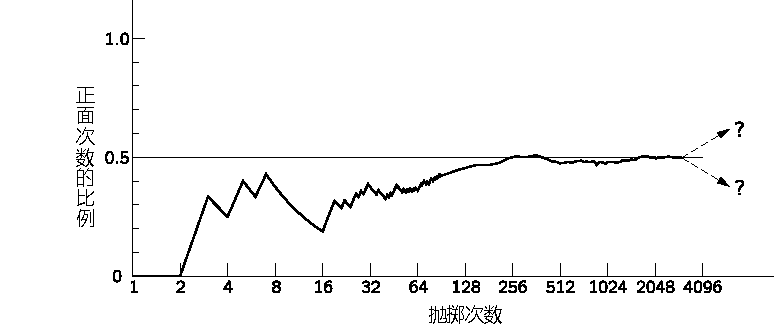
\includegraphics[width=0.35\textwidth]{Chapter6/获得正面的那些抛掷在某一特定次序中的比值}
    \caption{获得正面的那些抛掷在某一特定次序中的比值}
    \label{figure:获得正面的那些抛掷在某一特定次序中的比值}
\end{wrapfigure}
在图6.6中,我们根据本章前面提到的掷币记录画了一条表示比值$N_H/N$的曲线。从图中可以看出,对于大的$N$,得正面的比值趋向于接近0.5。遗憾的是,对任何给定的一轮或几轮,连观察到的偏差都\uwave{保证不了接近于预期}的偏差,总是有一定的机会出现大的起伏——一长串的正面或者一长串的反面——造成一个任意大的偏差。我们一切所能说的,只是\uwave{如果}偏差接近于预期的$1/2\sqrt{N}$(比如说在2或3倍之内),那么就没有理由去怀疑硬币的可靠性。如果偏差大很多,那么我们可以对硬币发生怀疑,但无法证明它是灌过铅的(或者抛掷者是非常机灵的!)。

我们也没有考虑过应该如何来处理这样一块“硬币”或某一与之相似的“不确定的”物体(比如一块始终以两种方位中无论那一种着地的石块),对于它们来说,我们很有理由认为出现正面和反面的概率应该是不同的。我们已经定义了$P(H)=\left < N_H \right >/N$。那么怎样知道$N_H$的\uwave{预期值}是多少呢?在某些情况下,我们所能做得最好的,就是去观察在大量抛掷中所得正面的数目。由于缺少任何更好的证据,我们不得不令$\left < N_H \right > = N_H\textrm{(观察值)}$。(除此之外,还能期望做什么呢?)然而必须理解到,在这样一种情况下,不同的实验或不同的观察者可能会推论出不同的概率$P(H)$。但是我们可以\uwave{预料},这些不同的答案应该在偏差$1/2\sqrt{N}$的范围内相互一致[加入$P(H)$接近于二分之一的话]。实验物理学家常常这样说:“实验确定的”概率是有“误差”的,并且把它写成
\begin{equation}
\label{Eq:I:6:14}
P(H)=\frac{N_H}{N}\pm\frac{1}{2\sqrt{N}}.
\end{equation}
在这样一个表达式中含有下列意义:\uwave{存在}着一个“真正的”或“正确的”概率,只要我们知道的东西足够多,就能把它计算出来,其次是由于有起伏,观察会发生“误差”。然而没有办法能使这种想法做到逻辑上始终如一。如果能领悟到下列几点或许要比较好一些,即概率概念在某种意义上是主观的,它总是建立在不肯定的知识上的,而且他的总量值是随着我们得到的信息越多而改变着的。


\section{概率分布}

我们现在回到无规行走的问题上来,并且考虑它的一种修正。我们设想除了每一步的方向(+或-)可以随机选择外,每一步的\uwave{长度}也能以某种无法预定的方式变化着,唯一的条件就是\uwave{平均而言}步子的长度是一个单位。这种情况更能代表像气体中一个分子的热运动那样的状况。如果我们称一步的长度为$S$,那么$S$完全可以取任何一个值,但最通常的是“接近于”1。为明确起见,我们令$\left < S^2 \right > = 1$,或者与之同等,$S_{\text{rms}}=1$。$\left < D^2 \right > $的推导将仿照以前一样,只是式(\ref{Eq:I:6:8})现在要加以改变而读作
\begin{equation}
\label{Eq:I:6:15}
\left < D_N^2 \right >=\left <D_{N-1}^2\right >+\left <S^2\right >=\left <D_{N-1}^2\right >+1.
\end{equation}

同以前一样,我们得到
\begin{equation}
\label{Eq:I:6:16}
\left <D_N^2\right > =N.
\end{equation}

现在对于距离$D$,我们会预期得到什么样的一种分布呢?比如在走了30步后,$D=0$的概率是多少?回答是$0$!$D$取\uwave{任一特定值}的概率是0。因为根本没有一种机会能使后退的(长度是变化的)步子的总和与朝前的步子的总和正好相等。我们无法画出一张像图6.2那样的图。

然而如果我们不是去问获得其值正好等于0, 1,或2的那些$D$的概率是多少,而代之以去问获得其值\uwave{靠近}0, 1,或2的那些$D$的概率有多大,那么我们就能得到与图6.2相似的曲线。我们定义$P(x,\Delta x)$为$D$位于$x$处一个间隔$\Delta x$(比如从$x$到$x+\Delta x$)内的概率。对于小的$\Delta x$,我们可以预期$D$位于这个间隔内的概率,与间隔的宽度$\Delta x$成正比。因此我们可以写成
\begin{equation}
\label{Eq:I:6:17}
P(x,\Delta x)=p(x)\,\Delta x.
\end{equation}
函数$p(x)$称为\uwave{概率密度}。

$p(x)$的形式与所走步子的数目$N$有关,也与个别步子的长度有关。我们不能在这里给出有关的论证,但当$N$很大时,对于所有合理的个别步子的长度分布,$p(x)$都是\uwave{相同}的。因而只取决于$N$。在图6.7中,我们对三个$N$值各作一条曲线,你们会注意到,这些曲线的“半宽度”(离$x=0$的典型散布范围)是$\sqrt{N}$,正如我们已证明过它理应如此。

\begin{figure}
    \centering
    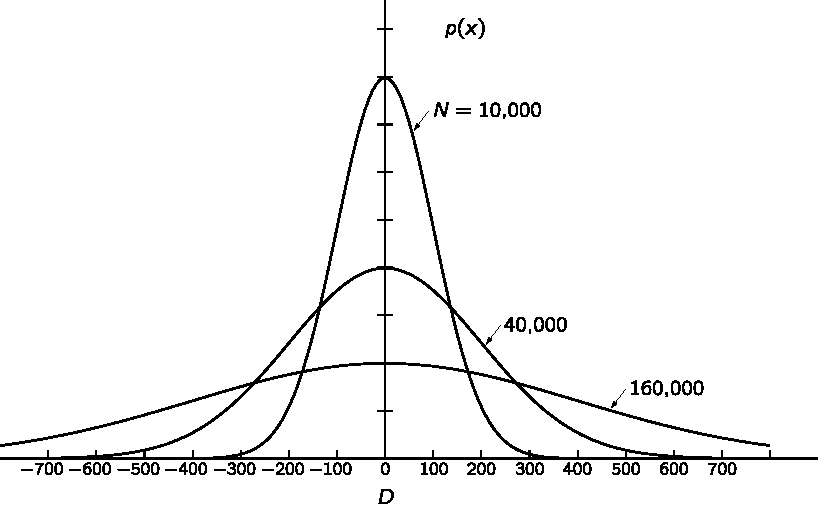
\includegraphics[width=0.55\textwidth]{Chapter6/在步数为N的无规行走中停止在从起点算起的距离}
    \caption{\footnotesize 在步数为$N$的无规行走中停止在从起点算起的距离$D$处的概率密度($D$是用方均根步长的单位来量度的)}
    \label{figure:在步数为N的无规行走中停止在从起点算起的距离}
\end{figure}

你们可能也已注意到,靠近零处的$p(x)$值反比于$\sqrt{N}$。这是由于曲线都有相似的形状以及曲线下面的面积都应相等而来的。既然$p(x)\Delta x$是当$\Delta x$很小时在$\Delta x$中找到$D$的概率,那么我们可以这样来确定在任意一个从$x_1$到$x_2$的间隔内\uwave{不论何处}找到$D$的概率,只要把间隔分割成许多微小增量$\Delta x$,然后对每个增量的有关概率$p(x)\Delta x$相加而求其总和。$D$落在$x_1$与$x_2$之间某处的概率,我们可以写作$P(x_1 < D < x_2)$,它等于图6.8中所示阴影的面积。增量$\Delta x$取得越小,结果就越正确。因此我们可以写成
\begin{equation}
\label{Eq:I:6:18}
P(x_1 < D < x_2)=\sum p(x)\,\Delta x=\int_{x_1}^{x_2}p(x)\,dx.
\end{equation}

\begin{wrapfigure}{r}{0.5\textwidth}
    \centering
    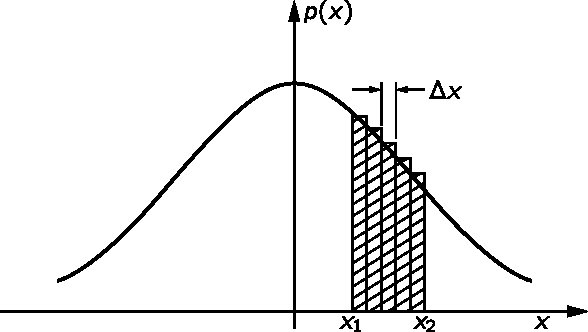
\includegraphics[width=0.35\textwidth]{Chapter6/无规行走中所通过的距离D,它位于x1与x2}
    \caption{\footnotesize 无规行走中所通过的距离$D$,它位于$x_1$与$x_2$之间的概率就是曲线$p(x)$下面从$x_1$到$x_2$的面积}
    \label{figure:无规行走中所通过的距离D,它位于x1与x2}
\end{wrapfigure}
整个曲线下面的面积是$D$落在不论何处(也就是它具有在$x=-\infty$到$x=+\infty$之间的\uwave{某一}值)的概率。这个概率当然是1。因而必须有
\begin{equation}
\label{Eq:I:6:19}
\int_{-\infty}^{+\infty}p(x)\,dx=1.
\end{equation}
由于图6.7中的曲线与$\sqrt{N}$成比例变宽,所以为了保持总面积等于$1$,它们的高度必须正比于$1/\sqrt{N}$。

我们这里所描述的概率密度函数是最经常遇到的一种,通常把它称为\uwave{正常}或\uwave{高斯}概率密度。它的数学形式是
\begin{equation}
\label{Eq:I:6:20}
p(x)=\frac{1}{\sigma\sqrt{2\pi}}\,e^{-x^2/2\sigma^2},
\end{equation}
其中$\sigma$称为\uwave{标准偏差},在我们的情况中$\sigma=\sqrt{N}$,或者当方均根步长不为1时,$\sigma=\sqrt{N}S_{\text{rms}}$。

前面我们已提到,气体中一个分子或任何一个粒子的运动犹如一种无规行走。假定我们打开一个装着有机化合物的瓶子,让它的一部分蒸气跑到空气中去。如果外面有气流,以致空气在作循环运动,那么气流也将带着蒸气一起运动。然而即使在\uwave{完全静止的空气}中,蒸气也会渐渐散布开去,进行扩散,直到布满整个空间。我们可以从它的颜色或气味加以鉴别。有机化合物蒸气的个别分子之所以能在静止空气中散布出去,是由于这些分子与其他分子碰撞而造成的分子运动所致。如果我们知道其“步子”的平均大小,以及每秒所走的步子,那么就能求出一个或$n$个分子在经过任何一段特定时间后在从其起点算起的某一距离被找到的概率。随着时间的消逝,步子越走越多,气体就会像图6.7中相继的几条曲线那样逐渐散开。在以后要讲的一章中,我们将求出步子的大小和步子的频率如何与气体的温度和压强有关。

我们以前说过,气体的压强是由于分子撞击容器壁而形成的。以后如果要作较定量的描写时,我们就需要知道分子在弹跳时跳得有多快,因为它们所作的碰撞与这个速率有关。然而我们不能说这些分子具有如何如何\uwave{确定的}速率,这里必须用概率来描写。一个分子可以具有任何一个速率,但有些速率出现的可能性比另一些要大。我们可以这样来描写气体内正在发生什么,这就是说处任何一个特定分子具有速率在$(v)$与$(v+\Delta v)$之间的概率$p(v)\,\Delta v$,而$p(v)$这个概率密度是速率$v$的一个确定函数。往后我们会看到,麦克斯韦如何运用常识和概率观念为$p(v)$找到一个数学表示式。函数$p(v)$的形状\footnote{麦克斯韦的表达式是$p(v)=Cv^2e^{-av^2}$,其中$a$是一个与温度有关的常数,而$C$应如此来选定,使总的概率等于$1$。}如图6.9所示。速度可以取任何一个值,但是最可能取的是靠近最可几值或预期值$\left < v \right >$的那一些。

\begin{wrapfigure}{r}{0.45\textwidth}
    \centering
    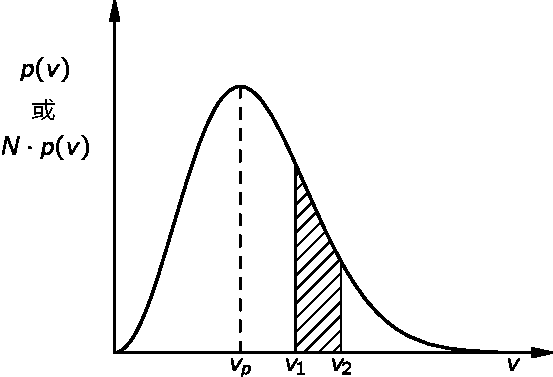
\includegraphics[width=0.35\textwidth]{Chapter6/气体中分子的速度分布}
    \caption{气体中分子的速度分布}
    \label{figure:气体中分子的速度分布}
\end{wrapfigure}

我们常常以稍微不同的方式去看待图6.9中的曲线。如果我们考虑一个典型容器(比如,其体积为1升)中的分子,那么容器中存在着极大数量的分子($N\approx10^{22}$)。由于$p(v)\,\Delta v$是\uwave{一个}分子具有在$\Delta v$间隔内的速度的概率,所以根据我们对概率的定义,我们说,找速度处在间隔$\Delta v$内的分子数其\uwave{预期值}$\left <\Delta N \right >$应是
\begin{equation}
\label{Eq:I:6:21}
\left <\Delta N\right >=N\,p(v)\,\Delta v.
\end{equation}
我们称$Np(v)$为“速度分布”。曲线下面两个速度$v_1$与$v_2$之间的面积,例如图6.9中所示阴影的面积代表了[对曲线$Np(v)$来说]速度在$v_1$和$v_2$之间的分子的预期数。由于在气体的情况中,我们通常与大量的分子打交道,所以可以期望这一面积与预期数的偏差是小的(犹如$1/\sqrt{N}$),因此我们常常不说“预期”数,代而说之:“具有速度在$v_1$和$v_2$之间的分子数\uwave{是}曲线下面的面积。”但是我们应当记住,这种陈述所谈到的总是\uwave{可几}数(probable numbers)。


\section{测不准原理}

在描写气体样品中$10^{22}$个或类似这样多个分子的行为时,概率的概念肯定是非常有用的。因为很清楚,即使要写下每个分子的位置或速度,这种试图也是不实际的,当概率最初运用这类问题时,大家曾认为这是一种\uwave{方便}——一种处理非常复杂的情况的方法。现在我们认为,概率的概念是描写原子事件所\uwave{必不可少}的。按照量子力学这个有关粒子的数学理论,在\uwave{说明}位置和速度方面总是存在着某种不确定性。充其量我们可以说,任何粒子只有一定的概率可以使它的位置接近某一坐标$x$。

我们可以这样来引进一个概率密度函数$p_1(x)$,使$p_1(x)\Delta x$为在$(x)$与$(x+\Delta x)$之间找到这个粒子的概率。如果这个粒子的位置被很好地限制在某个地方,比如说靠近$x_1$,那么函数$p_1(x)$就可能如图6.10(a)所示的曲线给出的那样。与之相似,我们必须用概率密度$p_2(v)$来限定粒子的速度,而$p_2(v)\Delta v$则表示能找到一个处于$v$与$v+\Delta v$之间的速度的概率,如图6.10(b)所示。

\begin{wrapfigure}{r}{0.45\textwidth}
    \centering
    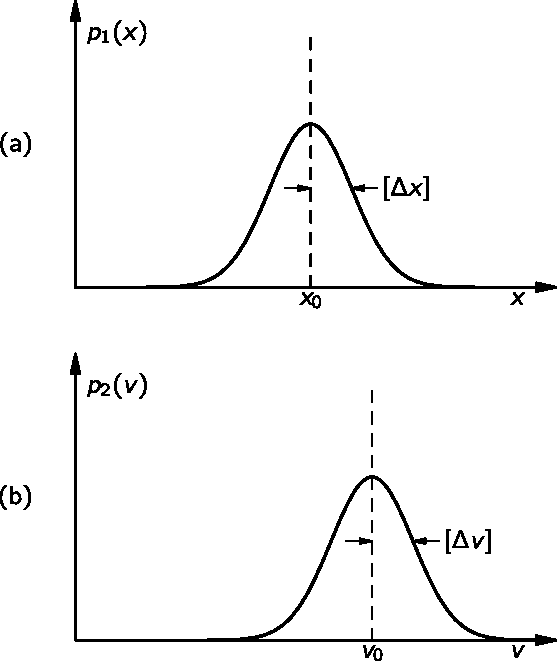
\includegraphics[width=0.35\textwidth]{Chapter6/观察一个粒子的位置与速度时的概率密度}
    \caption{观察一个粒子的位置与速度时的概率密度}
    \label{figure:观察一个粒子的位置与速度时的概率密度}
\end{wrapfigure}

量子力学的基本结果之一是:两个函数$p_1(x)$与$p_2(v)$不能予以独立选定,特别是不能把它们都取得任意的窄。如果我们称$p_1(x)$曲线的典型“宽度”为$[\Delta x]$,$p_2(v)$曲线的典型宽度为$[\Delta v]$(各如图所示),那么自然界就要求这两个宽度的乘积至少要与数$\hbar/2m$,其中$m$是粒子的质量。我们可以把这个基本关系写成
\begin{equation}
\label{Eq:I:6:22}
[\Delta x]\cdot[\Delta v]\geq\hbar/2m.
\end{equation}

这个式子就是我们前面提到过的\uwave{海森堡测} \uwave{不准原理}的一种表述。

由于式(6.22)的右面是一个常数,这就表明,如果我们迫使一个粒子处于某一特定位置而试图把它“钉住”,结果它就获得一个很大的速度。或者是:如果我们迫使它跑得很慢,或以精确的速度运动,那么它就要“散开”,以致我们不能很好地知道它究竟在那里。粒子的举止真是太奇妙了!

测不准原理描述了在叙述自然界的任何尝试中所必然存在着的那种内在的模糊性或不明确性。我们对自然界的最准确描写必须用\uwave{概率}的观念。有些人不喜欢用这种方法来描写自然界,不知怎么地,他们总觉得,只要能说出一个粒子\uwave{真正}在做什么,他们就能同时知道它的速度和位置。在量子力学发展的初期,爱因斯坦曾为这个问题十分担忧。他常摇头说:“啊!上帝肯定不是用掷骰子来决定电子应如何运动的!”他为这个问题担忧了好长时间,或许他从来也没有使他自己真正相信过这个事实,即:这是人们对自然界所能作出的最好描述。现在仍然有一、二位物理学家在研究这问题,他们从直觉上深信,可以通过某种方式用另一种方法来描写这个世界,并且可以把有关事物行为的所有这种不确定性都消除掉。然而到现在没有一个成功的。

当我们希望描写原子结构时,确定一个粒子的位置所必然要出现的不确定性就变得极为重要。在氢原子中有一个由单个质子组成的核,核的外面有一个电子,而这个电子的位置的不确定性就同原子本身一样大!因此我们不能严格地说:电子在某一“轨道”上绕质子运动,最多我们可以说,在一个离质子距离为$r$的体积元$\Delta V$内有一定的\uwave{机会}($p(r)\,\Delta V$)观察到这个电子,概率密度$p(r)$由量子力学来确定。对一个未受扰动的氢原子来说,$p(r)=Ae^{-2r/a}$,这是一个如图6.8所示的那种钟形函数。数$a$是“典型”的半径,函数由这里开始减小很快。既然在离原子核距离远大于$a$的地方找到电子的概率很小,我们可以把$a$设想为“原子的半径”,大约等于$10^{-10}$米。

\begin{wrapfigure}{r}{0.45\textwidth}
    \centering
    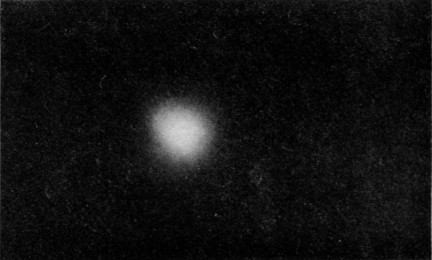
\includegraphics[width=0.35\textwidth]{Chapter6/使氢原子形象化的一种方法}
    \caption{\footnotesize 使氢原子形象化的一种方法。这里云的密度(洁白度)表示能观察到电子的概率密度}
    \label{figure:使氢原子形象化的一种方法}
\end{wrapfigure}
如果想像有这样一团“云”,它的密度正比于我们能观察到的电子的概率密度,那么我们就能形成氢原子的图象。这样一团云的一个实例如同6.11所示。所以我们对氢原子的最好“写照”便是一团“电子云”(虽然我们\uwave{实际}上指的是“概率云”)围绕着一个核。电子就处在云中某一地方,但自然界只允许我们知道在任何一个特定位置上能找到它的\uwave{机会}是多少。

在尽可能多地了解自然界的努力中,现代物理学曾发现,有些事情永远不可能确切地“知道”。我们的许多知识必然总是不确定的,而用概率来表述时,我们所能获得的知识则\uwave{最多}。


\chapter{万有引力理论}

\section{行星运动}

在这一章中,我们将要讨论对人类智慧影响至为深远的概括之一的引力定律。当我们现在赞颂人类智慧的时候,应当先停下来向\uwave{大自然}表示敬畏之意,因为她能如此完整而普遍地遵循引力定律这样一个出奇地简单的原理。那么什么是引力定律呢?它指出,宇宙中每一个物体都以一定的力吸引着每一个其他物体,而对任何两个物体来说,这一力正比于每一个物体的质量,而反比于它们之间距离的平方。这个称述数学上可以用下列式子来表示:
\begin{equation*}
F=G\,\frac{mm'}{r^2}.
\end{equation*}
如果对此再加上一个事实,即一个物体在力的作用下会沿着力的方向得到加速,而加速的快慢与物体的质量成反比;那么我们就已说出了所需要的一切,于是一个天资卓越的数学家就能推导出这两个原理的所有结论。然而由于你们还没有被认为天资如此卓越,所以我们要更详细地来讨论一下这些结论,而不是只给你们留下简单的原理。我们将简短地叙述一下发现引力定律的故事,讨论它的某些结果,它在历史上的作用,这样一条定律所遗留下来的神秘之处,以及爱因斯坦对这条定律所作的若干改进;我们还将讨论这条定律与物理学中其他定律的关系。所有这些不可能在一章中都讲到,所以有些论题将在适当的时候放到稍后的几章中去讨论。

故事要从古人对行星在恒星中间运动的观察,并且最终作出了它们在围绕太阳运行的推论开始,这是后来为哥白尼所重新发现的一个事实。行星究竟\uwave{怎样}围绕太阳运行,并且究竟用什么样的\uwave{运动}绕之运行,要发现这些,就要稍微多作一点工作。15世纪初叶,在行星到底是不是围绕太阳运行这个问题上曾有过激烈的争论。第谷•布拉赫(Tycho Brahe)有一个想法,它与古人提出的任何观点都不相同,他认为:如果能足够精确地测得行星在天空中实际的位置,那么这些有关行星运动本性的争论就会得到最好的解决。如果测量能精确地显示出行星在如何运动,那么或许有可能去建立这种或那种观点。这是一个非同小可的想法:如果要想发现什么东西,那么去细致地做一些实验要比展开冗长的哲学争辩好得多。在这个想法的指引下,第谷•布拉赫在哥本哈根附近的希恩(Hven)岛上他的天文台里,花了多年时间来研究行星的位置。他编制了一种篇幅庞大的星表;在第谷死后,数学家开普勒对这些星表进行了研究,从这些数据中,开普勒发现了涉及行星运动的一些非常优美、卓越而又简单的定律。



\section{开普勒定律}

开普勒首先发现,每个行星沿一条称为\uwave{椭圆}的曲线绕太阳运行,而太阳处在椭圆的一个焦点上。椭圆不仅仅只是一个卵形的东西,而是一条非常独特和精确的曲线,这条曲线可以用两只平头钉(在每个焦点上各钉一只),一束线和铅笔把它画出来;或者用数学术语来说,椭圆是(平面上)到两个定点(焦点)的距离之和是一个常数的轨迹。或者,如果你愿意的话,就把它说成是一个压扁了的圆吧(图7.1)。

\begin{wrapfigure}{r}{0.3\textwidth}
    \centering
    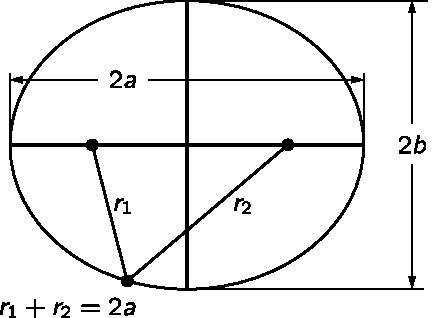
\includegraphics[width=0.25\textwidth]{Chapter7/椭圆}
    \caption{椭圆}
    \label{figure:椭圆}
\end{wrapfigure}
其次开普勒发现,行星并不以均匀速率绕太阳转动,而是当它们接近太阳时跑得较快,远离太阳时则跑得较慢,确切地说便是这样:设在任意相继的两个时间,比如说相隔为一周的时间内观察一个行星,并且对每个观察位置向行星画一条矢径\footnote{矢径是从太阳到行星轨道上任何一点的连线。}。那么行星在一周中所经过的轨道上一段弧线和两条矢径一起围成一定的平面面积,如图7.2所示的那个阴影面积。如果在离太阳较远的那部分轨道上(此时行星运动得较慢),也作时间相隔一周的与前类似的两次观察,那么这时围成的面积与前一情况下的面积完全相等。因此,按照开普勒第二定律,每个行星的轨道速率都使矢径在相等的时间内“扫过”相等的面积。

\begin{wrapfigure}{l}{0.3\textwidth}
    \centering
    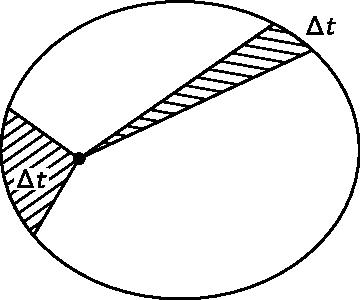
\includegraphics[width=0.25\textwidth]{Chapter7/开普勒的面积定律}
    \caption{开普勒的面积定律}
    \label{figure:开普勒的面积定律}
\end{wrapfigure}
开普勒第三定律发现得较晚,这条定律与前两条不同,各属于不同的范畴,因为它不是只涉及单独的行星,而涉及一个行星与其他行星之间的关系。这条定律表明:如果把任何两个行星的轨道周期和轨道大小进行比较,则周期与轨道大小的3/2次方成正比。这里所说的周期是行星在其轨道上完全绕一圈所需的时间间隔,而所谓轨道的大小使用椭圆轨道最大直径(术语叫“长轴”)的长度来量度的。更简单一些,如果行星绕圆周运动(实际上,它们也近于这样做),那么绕圆周走一圈所需的时间将正比于直径(或半径)的3/2次方。这样,开普勒三条定律便是:
\begin{enumerate}
\item[Ⅰ] 每个行星都沿椭圆轨道绕太阳运行,太阳位于各椭圆的其中一个焦点上。
\item[Ⅱ] 从太阳画到行星的矢径,在相等时间间隔内扫过相等的面积。
\item[Ⅲ] 任何两个行星的周期平方正比于它们各自轨道半长轴的立方:$T^2\sim a^2$。
\end{enumerate}


\section{动力学的发展}

当开普勒发现这些定律的时候,伽利略正在研究有关运动的定律。当时的问题在于什么东西使行星绕转运动(那时有一种理论这样说,行星之所以运行是因为在它们背后有看不到的天使在扑动它的飞翼,推动它们前进。你们将会看到,这个理论现在被修改了一下!这就是说,为了保持行星的绕转运动,看不见的天使必须朝与运动方向不同的方向飞行,并且它们也没有飞翼。除此之外,它倒多少有点像先前的理论!)在有关运动方面,伽利略发现了一个非常值得注意的事实,这个事实对于理解开普勒定律是必不可少的。这就是\uwave{惯性}原理——如果有某个物体在运动,但没有和其他东西相碰撞,也完全不受干扰,那么它将沿一直线以均匀速度永远运动下去。(\uwave{为什么}它能保持直线运动?我们不知道,但是事情就是如此。)

牛顿使这个观念更为明确,他说:“改变物体运动的唯一方法是要对之用\uwave{力}。”如果物体的速率变大,这必定有一个力施加在\uwave{运动方向上}。另一方面,如果物体的运动改变到另一个新的方向,那么它必定受到一个\uwave{斜向}的力作用。这样牛顿添进了如下一个概念:要改变一个物体运动的速率\uwave{或方向},就需要有力才行。例如:把一块石子系在绳上,使它旋转而作圆周运动,那么就需要有一个力以保持它在圆周上运行。这时我们必须把绳子\uwave{拉}住。事实上,这个定律说的是,力所产生的加速度反比于物体的质量;或者说,力正比于质量乘加速度。物体的质量越大,使它产生某一给定加速度所需的力就越大。(质量可以这样来测量,使其他石子系于同一根绳的末端,使它们以同样的速率绕同样的圆周转动,用这种方法可以知道它们所需的力的大小,质量较大的物体,所需的力较大。)从这些考虑中得出的一个卓越的观念就是:要保持行星在它的轨道上运行,根本不需要有一个\uwave{切向的力}(天使并不一定要沿切线方向飞行),因为行星总会沿所要求的方向运动,如果根本没有什么东西去干扰它,那么行星就将沿\uwave{直线}运行下去。但实际的运动却偏离了不存在力作用时物体所应沿之运动的那条直线,这种偏差差不多与运动相垂直,而不沿运动的方向。换句话说,由惯性原理得知,控制行星绕太阳运动所需的力不是一个\uwave{绕}太阳而是\uwave{指向}太阳的力。(如果有一个力指向太阳,那么当然太阳也许就是那天使了!)


\section{牛顿引力定律}

牛顿从他对运动定律的深入理解,意识到\uwave{太阳}可能是支配行星运动的那些力之渊源或机构所在,他给自己证明(或许我们不久也能证明),正是在等时间内扫过相等面积的这个事实,为所有偏离都是径向的这件事树立了一个明确的标志——也就是证明了面积定律是所有的力都精确地\uwave{指向太阳}这一观点的一个直接结果。

其次,对开普勒第三定律的分析可以表明,行星越远,作用力越弱。如果比较两个离太阳距离不同的行星,那么分析表明,力与行星各自的距离平方成反比。把这两条定律结合起来,牛顿于是推断说,必定存在着一个力,它的大小反比于两个物体间距离的平方,方向则沿着它们间的连线。

作为一个对事物普遍性有非凡触觉的人,牛顿当然要做出这种假设,认为这个关系可以更普遍地加以应用,而不只是限于太阳拉住行星这个事实。例如当时已经知道,正像月球绕着地球转动一样,木星也有自己的月球在绕着它转动,于是牛顿确信,每个行星都在用一个力拉住自己的月球。关于把\uwave{我们}吸住在地面上的那个力,牛顿也早已知道,所以,他就提出,这类力是一个\uwave{普遍存在}的力—— \uwave{每个物体都吸引任何其他一个物体}。

其次一个问题是,地球拉住人的力与它拉住月球的力是否“相同”,也就是说,是否都与距离平方成反比。如果地面上一个物体原来静止,然后释放,在第一秒内落下4.9米,那么在同样时间内,月球将落下多远?我们也许会说,月球根本没有落下。但是如果没有力作用在月球上,它会沿一直线离去,可是,它并不这样做而是沿一圆周运动,所以实际上它是从那个如果根本没有力作用时所应处的位置上\uwave{落}下来。从月球的轨道半径(约240,000英里)以及它绕地球一圈所需的时间(约为29天),可以算出月球在其轨道上每秒走了多远,随后就可以算出它在一秒钟内落下了多远\footnote{这就是说,月球的圆形轨道处在一根直线之下有多远,而这根直线就是对月球在一秒钟前在轨道上所处的那一点作的切线。}。经过计算这段距离约为$1/20$英寸。它与反平方定律吻合得非常好,因为地球的半径是4000英里,而如果,一个离地球中心4000英里的物体在第一秒内落下16英尺,那么一个在240,000英里,也就是在60倍远的地方的物体应当只掉下16英尺的$1/3600$,这个数值大约也为$1/20$英寸。为了想用类似的计算来检验这个引力理论,牛顿非常仔细地进行了他的计算,但是却发现差异很大,以至他认为这个理论与事实相矛盾,因为没有发表他的结果。六年之后,一个对地球大小的新的测量表明,天文学家曾使用了一个不正确的到月球的距离。当牛顿听到这个消息后,他就用正确的数据重新作了计算,所得的结果与事实非常一致。

\begin{wrapfigure}{r}{0.4\textwidth}
    \centering
    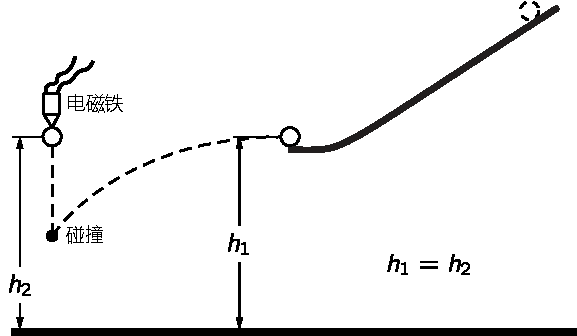
\includegraphics[width=0.35\textwidth]{Chapter7/演示垂直和水平运动互不相关的仪器装置}
    \caption{\footnotesize 演示垂直和水平运动互不相关的仪器装置}
    \label{figure:演示垂直和水平运动互不相关的仪器装置}
\end{wrapfigure}
月球“下落”的这种观念,多少有点使人迷惑,因为正像你们所知道的那样,月球丝毫没有靠近地球。但是这个观念相当有意思,以致值得进一步加以说明:所谓月球下落,其含义就是:它离开了不存在力的作用时原应遵循的那条直线。让我们举地球表面上的一个例子,一个靠近地面的物体被释放后,在第一秒内将降落16英尺,一个水平射出的物体也将降落16英尺;即使它沿水平方向运动,但在同样时间内它仍然要落下16英尺。图\ref{figure:演示垂直和水平运动互不相关的仪器装置}表示一个用以演示这一情况的仪器装置。

在轨道的水平部分有一个小球,它行将往前冲出一小段距离。在同一高度则有一个行将垂直下落的小球,另外,有一电动开关起控制作用,在第一个小球离开轨道的时刻,它随即释放另一个小球。至于两个小球在同样时间内落下同样的高度可以用它们在半空中相碰撞这个事实来证明。一个物体如子弹被水平射出时,可能在一秒钟内要跑很长一段路程——比如说2000英尺——但即使它是水平瞄准的,它仍然要落下16英尺。然而,如果我们把子弹发射得越来越快,那么会发生什么情况呢?不要忘记,地球的表面是弯曲的,如果子弹发射得足够快,那么在落下16英尺后,它可能恰巧在地面之上与之前相同的高度的地方。怎么会这样呢?子弹仍然在下落,但是由于地球向下弯曲,所以在“绕着”地球下落。问题是,它在一秒钟内必须跑多远才能使地球在水平线下面16英尺?在图7.4中,我们看到一个半径为4000英里的地球,以及一条在没有力作用的情况下子弹将循之而行的切向指向。
\begin{wrapfigure}{r}{0.35\textwidth}
    \centering
    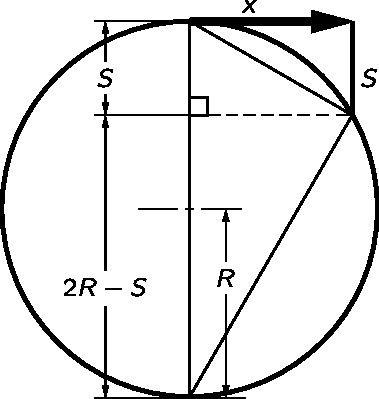
\includegraphics[width=0.3\textwidth]{Chapter7/指向圆形轨道中心的加速运动}
    \caption{\footnotesize 指向圆形轨道中心的加速运动。根据平面几何,$x/S=(2R-S)/x\approx 2R/x$,其中$R$是地球的半径(4000英里),$x$是每秒“水平通过”的距离;$S$是每秒“下落”的距离(16英尺)}
    \label{figure:指向圆形轨道中心的加速运动}
\end{wrapfigure}
如果我们现在应用几何学中一条奇妙的定理,即垂直于直径的半弦是所分割的直径两部分的比例中项,那么就可以看出,子弹所走的水平距离是所下落的距离16英尺与地球直径8000英里的比例中项。$(16/5280) \times 8000$的平方根很接近于5英里。于是我们看到,如果子弹每秒跑5英里时,那么它将继续以同样的速度每秒往地球落下16英尺,而决不会与之靠得更近一些,因为地球总是在不断地弯曲而离开子弹。加加林先生也是这样以每秒大约5英里的速率绕地球飞行25000英里来使自己保持在太空中的(他绕地球一周所需的时间稍微长一些,因为他在稍微高一点的地方飞行。)

只有在所获得的超过所给予的时,任何一个新定律的重大发现才有价值。现在,牛顿\uwave{用}开普勒第二和第三定律来推导他的引力定律,那么他都有那些\uwave{预言}?首先,他分析了月球的运动,因为他把地面上物体的下落与月球的下落联系起来了。接下来问题是它的\uwave{轨道是椭圆吗}?我们在往后的一章中将看到如何能精确地计算这个运动,而且人们确实能够证明,它的轨道应当是一个椭圆\footnote{这在本教程将不予证明。},所以毋需再用其他事实来说明开普勒\uwave{第一}定律,这样,牛顿作出了他第一个有力的预言。

引力定律解释了很多之前不能理解的现象。例如,月球对地球的吸引造成了潮汐,这在当时还是一个迷。月球把它下面的水吸引上来造成潮汐——这在以前人们也想到过,但是他们不如牛顿那样聪明,所以他们想一昼夜应该只有一次潮汐。其理由是,月亮把下面的水吸引上来,造成一个高潮和一个低潮。由于地球在月球下面旋转,就使一个地方的潮水每24小时涨落一次。实际情况是潮水每12小时涨落一次。另一个学派则主张,高潮应当在地球的另一面,他们争辩说,因为月球把地球从水中拉开!这两种理论都是错误的。实际的过程如下:月球对地球和对水的吸引在中心是“平衡”的,但是靠近月球的水被拉的程度要比平均值\uwave{大},而离月球较远的水被拉的程度要比平均值\uwave{小}。此外,水能流动,而比较结实和坚硬的地球却不能,真正的情况是这两种情况的结合。

\begin{wrapfigure}{r}{0.4\textwidth}
    \centering
    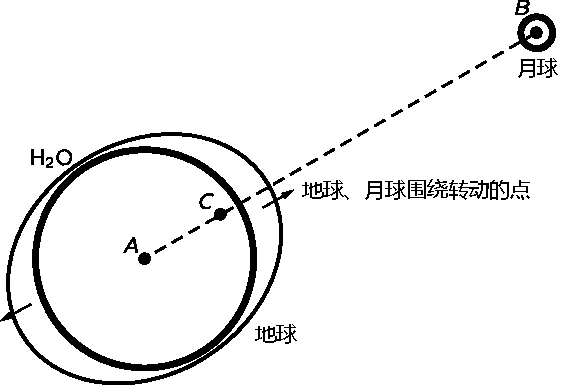
\includegraphics[width=0.35\textwidth]{Chapter7/解释潮汐现象的地球-月球系统}
    \caption{解释潮汐现象的地球-月球系统}
    \label{figure:解释潮汐现象的地球-月球系统}
\end{wrapfigure}
所谓“平衡”指的是什么意思呢?什么东西在平衡?如果月球把整个地球拉向自己,那么为什么地球不会“向上”落到月球上去?这是由于地球耍着像月球一样的花招,所以它在绕某点作圆周运动,这个点在地球内部,但不在地球中心。月球并不在绕地球转动,而是地球和月球一起在绕一个中心位置转动,每一个都在向着这个共同位置下落,如图7.5所示。这个绕共同中心的运动,是使每一个的下落得以平衡的原因。因此,地球也不是沿一直线行走,而是在绕一个圆周转动。地球上远的一边的水波是“不平衡的”,因为该处月球的引力要比在地球中心处小,而在地球中心处这一引力刚好和“离心力”平衡,结果这一不平衡使水沿离开地球中心的正方向运动。在近的一边,月球的吸引较强,所以不平衡是在空中相反的方向上,但又是\uwave{离开}地球的中心。最后,我们得到\uwave{两次}潮汐。



\section{万有引力}

当我们理解引力的时候,还可以理解别的什么呢?人人都知道地球是圆的。为什么地球是圆的?这很容易回答:由于引力的作用。我们之所以能够理解地球是圆的,仅仅是因为每个物体都在吸引任何其他的物体,所以地球尽它之所能把自身各部分相互吸引在一块!如果我们进一步深入下去,那么地球并非是一个\uwave{精确}的圆球,因为它在旋转着,从而引进了离心效应,在靠近赤道的地方,它趋向于与引力相对抗。其结果表明,地球应当是椭圆形的,而且我们甚至得到了这个椭圆的正确形状。这样,我们仅仅从引力定律出发,就能推论出太阳,月球和地球都应当是(近似的)圆球形。

应用引力定律我们还能做别的什么呢?如果我们看一下木星的月球,那么我们就能知道它们怎样围绕这个行星运行的一切情况。附带说一下,在有关木星的月球这个问题上曾经出现过一个困难,值得在这里一提。罗末(Roemer)非常仔细地研究了这些月球,他注意到,它们时而好像走在时间表的前面,时而好像走在时间表的后面。(等待很长一段时间,并找出这些月球绕行一圈平均所需的时间,就能找到它们的时间表。)当木星特别\uwave{靠近}地球时,它们走在前面,而当木星\uwave{远离}地球时,它们就走在\uwave{后面}。因而要按照引力定律来解释,看来这是一件非常困难的事——确实,如果找不到其他解释的话,这就会成为这个奇妙理论的终结。如果某条定律,只要在\uwave{一个}理应起作用的地方不起作用,那它\uwave{就是}错的。但是现在出现这个矛盾的原因是十分简单和美妙的:为了\uwave{看到}木星的月球就需要稍微花一点时间,因为光从木星跑到地球上来是需要时间的。当木星靠近地球时,它花的时间稍微少一点,而当木星远离地球时,所花的时间就稍微长一点。这就是为什么这些月球平均而论好像时而超前、时而稍微落后的原因,完全看它们靠近还是远离地球而定。这个现像表明光的传播并不是在一瞬间发生的,并且它第一次为光的速度提供了一个估计值,这个估计值是在1676\footnote{原文为1656,经查证为1676。——译者注}年做的。

\begin{wrapfigure}{r}{0.4\textwidth}
    \centering
    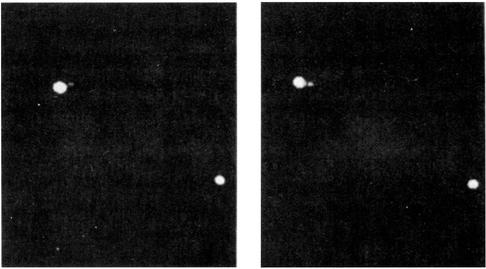
\includegraphics[width=0.35\textwidth]{Chapter7/双星系统}
    \caption{双星系统}
    \label{figure:双星系统}
\end{wrapfigure}
如果所有的行星彼此之间都相互吸引,那么控制一个行星比如说木星围绕太阳转动的力,不是只有从太阳来的引力,也有来自土星的拉力。实际上这个力并不强,因为太阳的质量比土星要大得多,但是毕竟有一点吸引作用,所以木星的轨道不应该是一个精确的椭圆,事实也确实是这样。它与正确的椭圆轨道稍有偏离,而且绕着它“摆动”。这样的运动就有点复杂了。人们曾视图在引力定律的基础上分析木星、土星及天王星的运动。对这些行星中的每一个,人们计算了它对其他行星所产生的效应,以便知道这些运动中出现的微小偏差与不规则性,是否单独用\uwave{这条}定律就能完全理解。好,就让我们看一下吧!对于木星和土星,一切都很好,但是对天王星却是“不可思议”的,它以非常奇特的方式运行着。至于它不是沿着一个精确的椭圆运行,那是可以理解的,因为有木星和土星在吸引它。但是,即使考虑到这些引力,天王星\uwave{仍然}没有按正确方式运行,所以引力定律就面临被推翻的危险,这是一个不能排除的可能性。但在英国与法国有两个人,亚当斯(Adams)与勒维耶(Le Verrier),他们各自设想了另一种可能性,或许存在着\uwave{另一个}幽暗而看不见的行星,以致人们从未看到过它,这个行星$N$可能在吸引天王星。他们计算了这样一个行星应处在那个位置才能造成所观察到的那个扰动。他们把这一消息分别通知有关的天文台,并说:“先生们,把你们的望远镜指向某某、某某位置,你们就会看到一颗新的行星。”至于人们对你注意不注意,那常常要看你在同谁进行联系。他们确实注意到了勒维耶;他们朝那个位置看了,果真发现有一颗行星$N$!另一个天文台过了几天也很快地看到了这颗新行星。

这个发现表明,牛顿定律在太阳系范围内是绝对正确的;但是这些定律能够扩展到离我们最近的相对距离较小那几个行星之外吗?第一个检验是回答这个问题:\uwave{恒星}是否也像行星一样在\uwave{彼此吸引}?在双星的情况下,我们有确凿的证据表明,它们是在彼此吸引。图7.6表示一对双星——两颗非常靠近的恒星(图上还有第三颗恒星,由此我们看出照片没有被偏转)。

图中也显示了双星在几年之后所在的位置,我们看到,相对于“固定”的恒星来说,双星的轴转过了一定角度,也就是说两颗星中每一颗在绕着另一颗转动。它们是不是在按照牛顿定律转动?图7.7表明对这种双星系统中一颗星的相对位置所作的测量。

这里我们看到一个完美的椭圆,测量工作从1862年开始,到1904年测完了整个一圈(到现在为止它必定又已绕行一圈多了)。一切与牛顿定律相一致,只是天狼星A\uwave{不再焦点上},为什么是这样?因为椭圆平面并不在“天空平面”上。我们不是从垂直方向去看轨道平面,而当从倾斜方向去看时,它还是一个椭圆,但焦点不再在同一个位置上。因此我们确实能够按照引力定律的要求来分析双星中一个绕另一个的运动。

\begin{figure}[htbp]
    \centering
    \begin{minipage}[t]{0.4\textwidth}
        \centering
        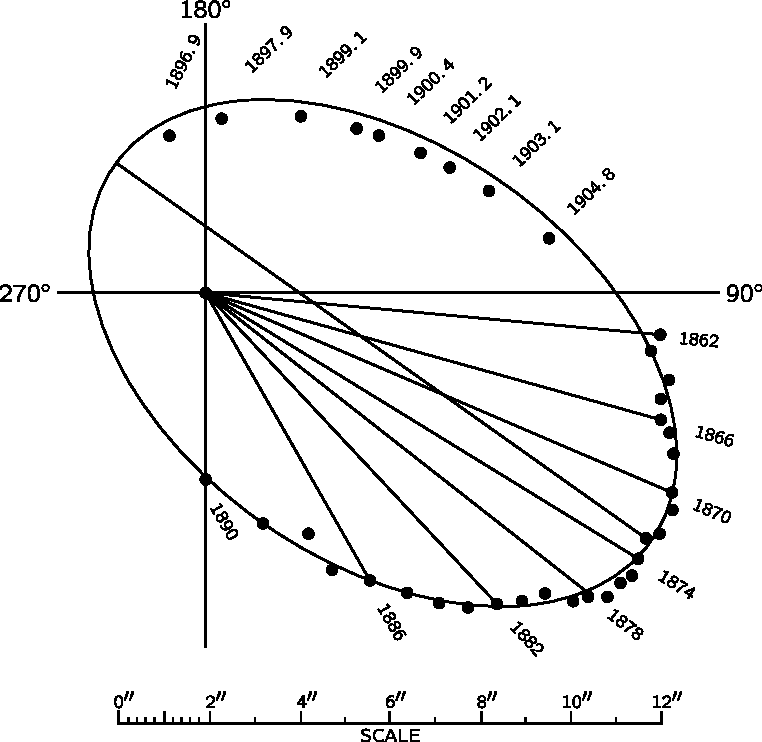
\includegraphics[width=5cm]{Chapter7/天狼星B绕天狼星A转动的轨道}
        \caption{天狼星B绕天狼星A转动的轨道}
        \label{figure:天狼星B绕天狼星A转动的轨道}
    \end{minipage}
    \begin{minipage}[t]{0.4\textwidth}
        \centering
        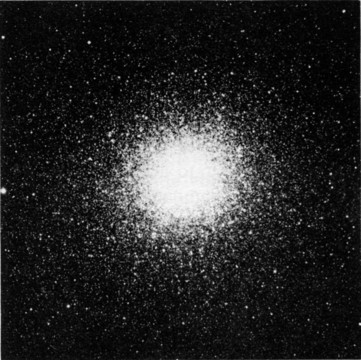
\includegraphics[width=5cm]{Chapter7/球状星团}    
        \caption{球状星团}
        \label{figure:球状星团}
    \end{minipage}
\end{figure}

\begin{figure}[htbp]
    \centering
    \begin{minipage}[t]{0.4\textwidth}
        \centering
        \includegraphics[width=5cm]{Chapter7/某星系}
        \caption{某星系}
        \label{figure:某星系}
    \end{minipage}
    \begin{minipage}[t]{0.4\textwidth}
        \centering
        \includegraphics[width=5cm]{Chapter7/星系团}    
        \caption{星系团}
        \label{figure:星系团}
    \end{minipage}
\end{figure}

甚至对更大的距离引力定律也是正确的,图7.8表明了这一点。如果一个人看不出引力在这里起作用,那他过于迟钝了。这幅图所显示的是天空中最美妙的事物之一——一个球状星团。所有的小点都是星星。虽然看上去它们好像向中心密集地挤成一团,其实这是由于我们的仪器难免发生错误所致。事实上,即使是最靠近中心的那些恒星之间的距离也非常巨大,而且它们也非常难得相互碰撞。在内部比在外沿有更多的恒星,越往外走,恒星越少。很明显,在这些恒星之间存在着一个引力。因此非常清楚,在如此巨大的、或许是太阳系大小的100,000倍的范围内也存在着引力的作用。让我们现在跑得更远一点,看一下图7.9所示的\uwave{某一银河系}的整体。这个银河系的形状表明它的物质明显地有团聚在一起的趋势。当然我们不能证明这一定律在这里也是准确地与平方成反比,而只能说明在如此巨大的范围内,仍然有一个引力作用着,它把整个物体聚集在一起。有人或许会说:“嗯,这一切真是太奇妙了,但是为什么不聚集成一个球呢?”回答是:因为它在\uwave{旋转},并且具有\uwave{角动量},而这是在它收缩时所不能放弃的;因此,它必然主要在一个平面内收缩(附带提一下,如果你想寻找一个合适的问题,那么银河系的旋臂如何形成,以及究竟是什么决定了这些银河系的形状等等,都还没有进行研究。)然而,非常清楚,银河系的形状来源于引力的作用,尽管它的结构的复杂性还不允许我们把它完全分析清楚。一个银河系的规模大约有50,000到100,000光年,地球到太阳的距离是$8\frac{1}{3}$光\uwave{分},所以你们可以看到这样的范围是多么的大!

正如图7.10所指出的那样,甚至在更大的范围内也存在着引力。图中还显示出有许多“小”的东西集成一簇,这就是一个犹如星团一样的\uwave{银河系团}。可见这些银河系相距如此之大也彼此吸引而同样聚集成团。或许甚至在超过\uwave{几千万}光年的距离之间也存在着引力作用,就我们今天所知,看来引力永远以与距离的平方成反比的方式延伸出去。

\begin{figure}[htbp]
    \centering
    \begin{minipage}[t]{0.4\textwidth}
        \centering
        \includegraphics[width=5cm]{Chapter7/星际尘埃云}
        \caption{星际尘埃云}
        \label{figure:星际尘埃云}
    \end{minipage}
    \begin{minipage}[t]{0.4\textwidth}
        \centering
        \includegraphics[width=5cm]{Chapter7/新星的形成}    
        \caption{新星的形成}
        \label{figure:新星的形成}
    \end{minipage}
\end{figure}


我们不仅能够理解星云,而且从引力定律出发,甚至还能对恒星的起源获得某些概念。如果我们有很大的一片尘埃与气体云,如图7.11所示,那么尘埃片与片之间由引力而产生的吸引,可能会使它们形成一些小的团块。在图上有一些“小”黑斑依稀可辨,它们可能是尘埃与气体相积聚的开始,而由于这些积聚物彼此间的引力作用,就开始形成星体。我们究竟是否看到过一个星的形成,这是一个可争论的问题。图7.12提供了一个证据说明我们曾经见到过。左边是一张1947年拍摄的照片,显示一个气体区域,中间有几个星体;右边是一张只过了7年之后拍摄的照片,显示两个新的亮点。气体是不是积聚了起来,引力是不是作用得足够强,并把它聚集成一个足够大的球体,以致在其内部发生星体核反应而把它变为一颗星呢?或许是这样,或许不是这样,而不近情理的是,仅仅在7年之中我们竟会如此幸运,能看到一颗星把本身转变为可见的形式;更不可能的是,我们居然一下子能看到两个!

\section{卡文迪什实验}

由前所见,引力作用伸展到距离极大的地方。但是,如果在\uwave{任何}一对物体之间有一个力作用着,那么我们应当能够测出作用在我们周围物体之间的这个力。比方说,难道不能用一个铅球和一个大理石球来做实验,观察大理石球朝向铅球跑去,而一定要去观察星体的相互绕行吗?用这样一种简单方式来做这个实验,其困难在于,这里的力是非常之弱的。因此必须格外小心地来对待,这就是说,要把仪器遮盖起来以避免与空气接触、要肯定它不带电等等;然后可以来测量这个力。卡文迪什(Cavendish)第一个进行了这种测量,他所使用的仪器的略图如图7.13所示。

\begin{wrapfigure}{r}{0.4\textwidth}
    \centering
    \includegraphics[width=0.35\textwidth]{Chapter7/卡文迪什测量引力常数的装置}
    \caption{卡文迪什用来验证小的物体之间存在万有引力和测量引力常数$G$的装置略图}
    \label{figure:卡文迪什测量引力常数的装置}
\end{wrapfigure}
这个实验第一次演示了两个大的固定铅球和两个小铅球之间力的直接作用;两个小铅球装在一根细杆的两端,细杆用一根非常精细的、称为扭丝的金属丝悬挂起来。用测量扭丝扭转了多少的方法,我们就能测出力的强度,证实它与距离平方成反比,并确定它的大小。这样,我们就能精确地确定公式
\begin{equation*}
F=G\,\frac{mm'}{r^2}.
\end{equation*}
中的系数$G$,因为质量和距离都是已知的。你们会说,“对地球来说我们早就知道这个系数了。”是的,但我们并不知道地球的\uwave{质量}。如果从这个实验知道了$G$,以及地球的吸引有多强,我们就能间接地知道地球的质量有多大!这个实验曾经叫做“称地球”实验。卡文迪什也声言他称了地球,但是他实际测量的是引力定律的系数$G$。这是唯一能确定地球质量的方法。$G$的数值是
\begin{equation*}
6.670\times10^{-11}\text{牛顿}\cdot\text{米}^2/\text{千克}^2.
\end{equation*}

引力理论的这一伟大成就在科学史上所产生的重大影响,怎么估计也不会过分。请把早先年代里无休止的争论和悖论盛行,知识中充满着混乱、迷惑以及不完善和不可靠这种情况同这条定律的明晰和简单做个比较吧!——现在,所有月球、行星和恒星都由这样一条\uwave{简单的规则}来支配,并且,人们能够理解它,从它推论出行星应当如何运动!这是科学在以后年代里所以会获得如此巨大成就的原因,因为它为人类理解宇宙间其他现像提供了一个希望,可能也有这样一种特别简单的定律来支配它们。


\section{什么是引力}

然而这条定律确实是如此简单吗?什么是它的机制?我们所做过的一切,不过是描写了地球\uwave{怎样}绕太阳运行,但是我们没有谈到是\uwave{什么东西在使它运动}。牛顿对此没有做过任何假设;他满足于找出它做的是\uwave{什么},而并不深入到它的机制中去。从那时起也没有人提出过任何机制。物理定律的特征,就是它们具有这种抽象的性质。能量守恒定律是一条关于这样一些量的定理,对于这些量必须加以计算,然后把它们加起来,但它没有提到它的机制;同样,力学的那些重要定律也是一些数学定律,我们并不知道起作用的机制是什么。为什么我们能用数学来描述自然,而在其背后有没有一个机制呢?无人知道。我们必须继续照此办理,因为用这种方法我们能够发现更多的东西。

引力的机制曾经屡次为人们所提到过,研究了一下很多人一再想到的其中的一个,是颇有趣味的。起初,当有人“发现”它的时候,确实非常高兴,感到十分幸运,但他随即发现原来这是错误的。这个机制大约在1750年第一次被人们提出。设想有许许多多粒子在空间以极大速度向各个方向运动,在它们穿过物质时只有很少一部分被吸收掉,当它们被吸收时,就给地球以一个冲量。然而,由于在一个方向上运动的粒子同在别的方向上运动的粒子一样多,所以这些冲量都互相抵消。但是来自太阳的粒子比来自另一边的粒子要少一些。因此,地球最后受到一个朝向太阳的冲量,而且,不要花费多少时间人们就能看出,这个冲量与距离的平方成反比,因为当距离改变时,太阳所张的立体角也要改变。这个机制错在那里呢?错在其中包括了一些新的结果,而这些新的结果是不\uwave{真实}的。这个特别的想法遇到了如下困难:地球绕太阳运行时,它与从前面射来的粒子相碰撞的次数,将比从后面射来的粒子要多。(当你在雨中奔跑时,打在你脸上的雨点要比打在你脑后的多!)因此从前面将给予地球更大的冲量力,而地球将会受到一种\uwave{对其运动的阻力作用},这种阻力使它在轨道上的运动减慢下来。人们可以算出,作为这种阻力的结果,地球需要多长时间才会停下来,结果是地球仍留在轨道上的时间并不长,所以这个机制行不通。从此也就没有再提出过任何一个机制,它既能“解释”引力,又不致于会预言其他实际\uwave{不}存在的现像。

其次我们要讨论万有引力与其他作用力之间可能存在的关系。目前还没有一种用其他力来说明引力的解释。它不是电或诸如此类的一个方面,所以我们无法解释。然而,引力和其他力十分相似,因而看一下它们的相似之处是很有趣的。例如,两个带电体之间的电力看上去就很像引力定律:它们之间的电力等于一个带负号的常数乘以电荷之积,并与距离的平方成反比。电力的方向则与引力的情况相反——同号相斥。但是两条定律含有同样的距离函数,这难道还不够引人注目?引力与电力之间的关系或许比我们所能想像的要密切得多。人们做了许多尝试试图把它们统一起来;所谓的统一场论不过是一个想把电力和引力结合起来的非常美妙的尝试而已;但是如果把引力与电力相比较,那么最有趣的事是力的\uwave{相对强度}。任何一个包括它们两者的理论,必须也能推导出引力有多大。

如果我们来看用某些自然单位表示的由于电作用产生的两个电子(自然界中的电荷的基本单位)之间的斥力,以及两个电子由于它们的质量而产生的引力,那么我们就能求出电斥力与万有引力的比值。这个比值与距离无关,是自然界的一个基本常数,如图7.14所示。两个电子间的万有引力与电斥力之比等于1比 \num{4.17d42} !现在的问题是,这样巨大的数字从何而来?正像地球与跳蚤的体积之比那样,这个数值不是偶然的。这个大得难以置信的数字是一个自然常数,所以它包含了自然界中某种深邃的性质。这样一个惊人的数字从哪里来呢?有些人说,总有一天我们会找到一个“宇宙方程”,其中的一个根就是这个数。要找到这样的方程,它确能以大得如此出奇的数字为一个自然根,那是非常困难的。人们也曾想到过其他的可能性;其中之一是把它与宇宙年龄联系起来。很清楚,我们必须在某个地方找到\uwave{另一个}巨大的数字。那么,我们是不是用\uwave{年}来表示宇宙的年龄呢?不,因为年不是“自然”量;它只是人们所想像出来的。作为某种自然量的一个例子,让我们来看一下光穿过一个质子的时间,它是 \numb{d-24}秒。如果我们把这个时间与 \uwave{宇宙年龄} \numb{2d10}年相比较,那么答案是 \numb{d-42}。它有大约相同数目的零跟在后面,因而有人提出,引力常数与宇宙年龄有关。如果情况真是如此,引力常数就会随时间而变化,因为随着宇宙的变老,宇宙年龄与光穿过一个质子所需的时间之比就会逐渐变大。

那么,引力常数是否可能随着时间\uwave{在}发生变化呢?当然,这种变化如此之小,以致要确定它是相当困难的。

\begin{wrapfigure}{r}{0.4\textwidth}
    \centering
    \includegraphics[width=0.35\textwidth]{Chapter7/两个电子之间的电力相互作用和引力相互作用的相对强度}
    \caption{两个电子之间的电力相互作用和引力相互作用的相对强度}
    \label{figure:两个电子之间的电力相互作用和引力相互作用的相对强度}
\end{wrapfigure}
这里我们能够想到的一个检验方法是确定在过去 \numb{d9} 年中这种变化可能产生过什么影响。\numb{d9}年大约是地球上出现最早的生命以来到目前为止的时间,是宇宙年龄的十分之一,在这段时间内,引力常数可能增加大约百分之三十,从这里可以得出,如果我们考虑到太阳的结构——即太阳物质的重量与其内部产生辐射能的快慢的平衡,那么我们可以推论说,如果引力增加百分之十,则太阳的亮度要增加比百分之十大得多——即引力常数的\uwave{六次方}。如果我们计算一下,引力改变时地球轨道会发生什么情况,那么我们将发现,地球那时已更\uwave{靠近}太阳。总而言之,地球将变得更热(大约摄氏100度),所有的水不会再留在海洋里而变成了充满在空气中的水蒸汽,这样,生命也就不会从海洋里开始。所以我们现在并\uwave{不}相信,引力常数是随着宇宙的年龄而改变的。但是,这样一些论证像我们刚才所给出的那样,是不会十分令人信服的,这个问题还没有完全得到解决。

众所周知,物体的重量正比于它的质量,而这种质量实质上就是惯性的一种量度,也就是当一个物体作绕圆周运动时,要维持它在圆周上有多难的一种量度。因此,若有一轻一重两个物体,由于重力作用而绕一更大的物体沿同一个圆周以同样速度转动,那么它们总将保持在一起,因为要在圆周上运动就\uwave{需要}力,对大的质量,需要的力也大。这就是说:对于一个较重的物体,重力作用应当\uwave{正好以恰当的比例}增加,所以这两个物体仍将一起做圆周运动。如果一个物体原先在另一物体的里边,那么它将\uwave{留在}里边而不离开;这是一个完全的平衡状态。因此,加加林或季托夫发现宇宙飞船舱内的一切东西是“失重”的,比方说如果他们碰巧丢掉一支粉笔,那么粉笔将与整个宇宙飞船沿着一条完全一样的路径绕地球飞行,所以它将始终在空间悬浮于宇航员的眼前。非常有趣的是,重力以极大的精密度\uwave{精确地}与质量成正比,因为如果不是如此的话,将产生某种效应,其中惯性与重量会有所区别。这样一种效应实际上并不存在。关于这一点,人们曾以极大的精密度用实验验证过,厄缶(fǒu)(E\"otv\"os)在1909年第一次进行了这种实验,而最近则由迪凯(Dicke)做过。对于所有做过实验的物质,它们的质量和重量的正比关系精确到了十的九次方之一或者更小,这真是个了不起的实验啊。



\section{引力和相对论}

另一个值得讨论的论题是爱因斯坦对牛顿引力定律所作的修正。尽管牛顿引力定律创造了所有这些惊人的成就,但仍然是不正确的!爱因斯坦对它所作的修正,在于把相对论考虑了进去。依照牛顿的观点,引力效应是瞬时发生地,也就是说,如果我们移动一个物体,那么我们就会立即感觉到一个新的力,因为物体到达了新的位置;按照这种说法,我们可以以无穷大的速度发送信号。然而爱因斯坦提出了种种论证,说明我们不能发送比光更快的信号,所以牛顿引力定律必定是错误的。在考虑到延迟情况而加以校正后,我们得到一条新的定律,称为爱因斯坦引力定律。这条非常容易理解的新定律的一个特点是:在爱因斯坦相对论中,任何具有\uwave{能量}的东西也具有质量——质量应在这一意义下来理解,即它以引力方式被其他质量所吸引。即使是光,由于它有能量,也就是有“质量”。当一束带有能量的光经过太阳附近时,它将受到太阳的吸引。所以光并不是沿直线行进的,而是被弯曲了的。例如在日食时,太阳周围的恒星应该看起来好像从它们的那些位置偏离出去了,这些位置就是如果太阳不在那里它们所应处的地方。而人们也观察到了这个情况。

最后,让我们把引力理论与其他理论比较一下。近年来我们发现,所有物质都由微小粒子所构成,并且世界上存在着几种相互作用,如核力等等。但是在这些核力或电力中还没有发现有那一个能用来说明引力。大自然的另一方面量子力学还没推广到万有引力。当尺度小到需要考虑量子效应时,引力效应是如此的微弱以至于根本没有必要发展一种有关万有引力的量子理论。另一方面,为了物理理论的内在一致性,重要的一点是看看是否牛顿定律修正为爱因斯坦定律之后,还可不可以进一步加以修正,使之与测不准原理相协调。到目前为止还没有完成这最后的修正。


\chapter{运动}

\section{运动的描述}

为了找出物体随时间而发生的各种变化所遵循的规律,我们必须\uwave{描述}这些变化,并用某种方式把它们记录下来。在物体中要观察的最简单的变化是物体的位置随时间的明显改变,我们把它称之为运动。让我们考虑一些固体吧,它们身上带有一个固定的可观测标记,这个我们后面会称之为点。我们将讨论这个小标记的运动(这个小标记可以是一辆汽车的散热器盖子,或一个下落的球的球心),并将试图描述它在运动以及如何运动这一事实。

这些例子看来似较平庸,但在描述其变化时,也有许多要小心对付之处。有些变化,例如,一朵缓慢漂移但迅速形成或迅速蒸发的云的漂移速率,或者一个女人思想上的变化,要描述它们就比描述在固体上一点的运动困难得多。我们不懂得分析思想上发生变化的简单方法,不过由于云可以用许多分子来表示或描述,或许在原则上我们能够通过描述云中所有个别分子的运动来描述云的运动。同样,或许思想上的变化甚至也与大脑内原子的变化有类似之处,但我们对此尚一无所知。

总而言之,这就是我们为什么要从点的运动开始研究的原因;也许我们应当把它们想像为原子,但在开始时粗糙一些可能更妥当。我们把它们简单地想像为某一类小的物体——所谓小,是指与运动的距离相比较而言。比如,在描述一辆开过一百公里的汽车的运动时,就不必区分汽车的前部和后部。的确,这里有一点差别,但粗略的看我们只讲“汽车”的运动,同样,我们选择的点不是绝对的点也丝毫没有关系;就我们现在的目的来说,没有必要极其精确。还有,在初次考察这个课题时,我们将不考虑世界的三维性。我们将只集中注意一个方向上的运动,就像在一条公路上行驶的汽车那样。当我们知道了如何描写一维运动后,就将回到三维中去。现在,你们会说:“这尽是一些琐碎的事。”确实如此。那么,我们怎样来描述这样的一维运动,比方说,汽车的运动呢?没有比这更简单的了。有许多可能的方式,下面是其中之一,为了确定不同时刻汽车的位置,我们测量它与起点的距离,并记下所有的观测。在表8.1中,$s$表示汽车离起点的距离,单位是英尺,$t$表示时间,单位是分。表中的第一行表示零距离和零时间——即汽车尚未出发。一分钟后,出发并开过了1200英尺。在两分钟内,它开得更远——注意汽车在第二分钟开过了更大的距离——并且加速前进;但在第三和第四分钟或者甚至一直到第五分钟之间发生了一些情况——也许是遇到红灯停了下来?然后它再次加速,在第六分钟末开过13000英尺,在第七分钟末开过18000英尺,在第八分钟开过23500英尺,在第九分钟它只前进到24000英尺,因为在最后一分钟它被警察拦住了。

\label{tab:表8.1}
\noindent
\begin{minipage}{\textwidth}
\begin{minipage}{0.3\textwidth}
\begin{table}[H]
    \centering
    \medskip 
    \scalebox{0.82}{
    \begin{tabular}{@{}ll@{}}
    \toprule
    $t$(分) & $s$(英尺)  \\ \midrule
    0 & 0     \\
    1 & 1200  \\
    2 & 4000  \\
    3 & 9000  \\
    4 & 9500  \\
    5 & 9600  \\
    6 & 13000 \\
    7 & 18000 \\
    8 & 23500 \\
    9 & 24000 
    \\ \bottomrule
    \end{tabular}
    }
    \caption*{表 8.1}
\end{table}
\end{minipage}\hfill
\begin{minipage}{0.7\textwidth}
\begin{figure}[H]
    \centering
    \includegraphics[width=0.75\linewidth ,totalheight=0.8\textheight , keepaspectratio]{Chapter8/汽车的距离-时间曲线}
    \caption{汽车的距离-时间曲线}
    \label{figure:汽车的距离-时间曲线}
\end{figure}
\end{minipage} 
\end{minipage} 


\label{tab:表8.2}
\noindent
\begin{minipage}{\textwidth}
\begin{minipage}{0.3\textwidth}
\begin{table}[H]
    \centering
    \medskip 
    \scalebox{0.9}{
    \begin{tabular}{@{}ll@{}}
    \toprule
    $t$(分) & $s$(英尺)  \\ \midrule
    0 & 0     \\
    1 & 16  \\
    2 & 64  \\
    3 & 144  \\
    4 & 256  \\
    5 & 400  \\
    6 & 576 
    \\ \bottomrule
    \end{tabular}
    }
    \caption*{表 8.2}
\end{table}
\end{minipage}\hfill
    \begin{minipage}{0.7\textwidth}
        \begin{figure}[H]
            \centering
            \includegraphics[width=0.75\linewidth ,totalheight=0.8\textheight , keepaspectratio]{Chapter8/落体的距离-时间曲线}
            \caption{落体的距离-时间曲线}
            \label{figure:落体的距离-时间曲线}
        \end{figure}
    \end{minipage} 
\end{minipage} 

这就是一种描写运动的方式,另一种方式是借助于图画。如果我们以横轴表示时间,纵轴表示距离,就得到如图8.1那样的一条曲线。当时间增加时,距离也增加,开始很慢,然后很快,在四分钟前后又很慢,以后几分钟内又再加快,最后在九分钟时,看来像停止增加了。这些情况不用表也能从图上观察到。显然,为了描述完全起见,人们还知道,在那些半分钟的标记处,汽车开到了那里。但是我们假定这个曲线图可以这样来解释,在所有的中间时刻汽车都具有某个位置。

汽车的运动是复杂的,另外我们举一个遵循简单的法则以简单的方式运动的例子,比如说一个下落的小球。表8.2列出了落体的时间(以秒为单位)和距离(以英尺为单位)。在零秒时,小球从零英尺开始下落,在第一秒末落下16英尺,在第二秒末落下64英尺,在第三秒末落下144英尺,等等。如果将表上的数字作图,就得到图8.2所示的一条漂亮的抛物线。这条曲线的公式可以写成
\begin{equation}
\label{Eq:I:8:1}
s=16t^2.
\end{equation}
这个公式使我们可以计算小球在任何时刻的距离。你们或许会说,对第一个曲线图也应当有个公式。实际上,人们也可以抽象地把这样一个公式写成
\begin{equation}
\label{Eq:I:8:2}
s=f(t),
\end{equation}
它表示$s$是某个依赖于$t$的量,或用数学术语来说,$s$是$t$的函数。由于我们不知道这个函数是什么,因此无法以确定的代数形式写下来。

现在我们已经看到了两个用非常简单的思想就能适当地描述的运动的例子——没有什么难以捉摸之处。然而,难以捉摸之处还是有的,\uwave{有几处}。首先,\uwave{时间}和\uwave{空间}究竟意味着什么?结果表明,这些深刻的哲学问题在物理学上必须十分小心地加以分析,而着并不是容易做到的。相对论表明我们关于空间和时间的观念并不如人们乍一看来可以想像的那么简单。然而,就我们当前的目的而论,对我们在开始时所要求的精确度来说,我们毋需十分小心地去精确定义事物。或许你们要说:“这很糟糕,我听说过在科学上我们必须静确定定义每一件事。”我们不可能精确地定义\uwave{任何事物}!如果强求如此,只会使我们陷入像某些哲学家那样的思想僵化,他们面对面坐着,一个对另一个说:“你不知道你在讲些什么!”第二个说:“你所谓的‘\uwave{知道}’是什么意思呢?你所谓的‘\uwave{讲}’是什么意思呢?你所谓的‘\uwave{你}’又是什么意思呢?如此之类。”为了能够进行建设性的讨论,我们必须一致赞同我们所谈论的大致是同一件事。你们对于时间的了解已能满足我们目前的需要,但必须记住,还有一些微妙和难以捉摸的事情需要讨论,我们将在以后进行。

前面所涉及的另一个难以捉摸之处是能够设想我们正在观察的动点总是位于某处(当然,当我们注视它时,它在那里,但当我们看别处时,它可能不在那儿了。)现在知道,在原子的运动中,这个观念也是错误的,我们不可能在一个原子上找到一个标记并观察它的运动。这种微妙的情况我们将在量子力学中去仔细讨论,但是在引进复杂性之前,我们将首先了解一下这些问题是什么,\uwave{然后}才能较好地按照这个题材的更现代的知识进行修正。因此,关于时间和空间,我们将采用一种简单的观点。我们大致知道这些概念是怎么一回事,而那些驾驶汽车的人则知道速率指的是什么。

\section{速率}

尽管我们知道大概“速率”的意思,但这里还是有一些比较深的奥妙;要知道博学的希腊人也从未能恰当地描述牵涉到速度的问题。这奥妙就在于准确地理解到底什么才是“速率”,希腊人对这个问题感到很困惑,这是因为要发现一个新的数学分支才能解决这个问题,而这是超越于希腊人、阿拉伯人与巴比伦人固有的几何学与代数学之外的 。作为这个难点的一个例证,试用纯代数方法来解这样一个问题:一个气球正在膨胀,它的体积以每秒100厘米的比率增加;当气球体积为1000$\text{厘米}^3$时,气球半径增加的速率是多少?希腊人多少有点被这样的问题弄糊涂了。当然,这是被某些思想混乱的人所促成的。为了指出在某一时刻有关速度方面的推理上存在着困难,芝诺(Zeno)提出了一大堆佯谬,我们将举其中的一个来说明他的关于思考运动时存在着明显困难的论点。“请听这样的论点”,他说:“阿基利斯(Achilles)比乌龟跑得快10倍,但他却永远抓不住乌龟。因为,假定他们开始赛跑时,乌龟在阿基利斯前面100米,那么当阿基利斯跑了100米而到达乌龟原来所在的地方时,乌龟已经以他的快慢的$1/10$前进了10米。现在,阿基利斯又得跑另一个10米以便赶上乌龟,但在到达跑步的终点时,他发现乌龟仍在他前面1米;当他再跑1米时,他又发现乌龟依然在他前面10厘米,如此下去,\uwave{直至无穷}。因此,在任何时刻乌龟总是在阿基利斯前面,阿基利斯永远追不上乌龟。”这段论证错在那里?它错在认为一段有限的时间可以被分为无限多的小份,正如一条线段不断地一分为二分成无限多的小段一样。因此,虽然(在论证中)直到阿基利斯追上乌龟可以分成无穷多步,但是并不意味着是无穷无尽的\uwave{时间}。从这个例子我们可以看到,在有关速率的理解上,还是有所玄机的。

为了以更为清楚的方式来领会这所谓的玄机,我讲一个你们肯定听到过的笑话。坐在汽车里面的一位太太在某个地点被警察拦住了,警察走过来对她说:“太太,你刚才的车速是每小时60英里!”她反驳道:“先生,这是不可能的,我刚才只开了七分钟。这正是天大的笑话!我开车还没有到一个小时,怎么可能每小时走60英里呢?”假如你是警察的话你该如何回答她呢?当然,如果你真是那个警察,那就没有什么疑难之处;很简单,你会说:“对审判官讲去!”但是,假若我们没有这条退路,并且更公正和理智地对待这个问题,企图向这位太太解释所谓她的车速达每小时60英里的说法是什么意思,那么我们的含义\uwave{究竟}是什么呢?我们可以说:“太太,我们的意思是:如果你继续像现在这样开车,在下一个小时里你将开过60英里。”她会答道:“嗯,我的脚已经离开油门,汽车已慢了下来,所以如果我继续这样开下去,不会超过60英里的。”或者,我们考虑一个自由下落的小球,如果这个小球保持它正在进行的运动方式的话,我们想要知道它在第三秒时的速率有多大。这意味着什么呢?是继续\uwave{加速},落得更快吗?不,应该是继续以同样的\uwave{速度}运动。但这正是我们试图加以定义的东西!因为如果小球保持它现在正在进行的方式运动,那么它在以后就将继续保持这种方式运动。于是我们就需要更好地定义速度,究竟是什么必须保持一样呢?这位太太也可以这样来辩护:“如果我再继续保持现在的开车方式,那么过了一个小时后,我就会撞到街道尽头的墙上了!”看来要说清楚我们的意思并不那么容易。

许多物理学家认为测量是唯一定义任何事物的方式。那么,显然,我们应当使用测量速率的仪器——速度计,并说:“!太太,你的速度计的读数指到60。”可是她说:“我的速度计坏了,根本不能读数。”这是否表示汽车停着不动呢?我们相信,在我们造出速度计之前,就存在某种要测量的东西。只有这样,我们才可以说:“速度计走得不准,”或“速度计坏了。”如果速度脱离了速度计就没有意义了,那这么讲就毫无道理了。所以,显然在我们的头脑中存在着一种与速度计无关的概念,速度计只是用来使这个概念计量化罢了。所以,还是让我们来看看是否能得到比这个想法更好的定义。我们可以说:“嗯!固然在你的车子开了一个小时以前,你就会撞到墙上,但是如果你开了一秒钟,你就会通过88英尺的距离。太太\footnote{这一定是苏格拉底的太太。。},你刚才的车速正是每秒88英尺,如果继续下去,下一秒也将开过88英尺,而那堵墙离这还远着呢。”她就说:“对,但是,没有一条法律禁止每秒88英尺的车速!只有一条禁止每小时开60英里的法律。”“不过”我们反驳道:“这是同一件事。”如果这\uwave{确实是}同一件事,那就毋需赘言每秒88英尺了。事实上,自由落体甚至连一秒钟也不可能保持同样的运动方式,因为它的快慢在变化着,我们必须设法来定义速率了。

现在看来,我们已经走上正规了,似乎可以这样说:如果那位太太在另一个$1/1000$小时内继续这样行驶,她将开过60英里的一千分之一。换句话说,她毋需继续开足一小时,主要在于,\uwave{在某一瞬间}她正以这个速率开车。现在我们的意思是,只要她再多开一点点时间,那么汽车所通过的外加距离就和一辆以每小时60英里的\uwave{稳定}速率开动的汽车相同。也许每秒88英尺的观念是正确的,我们看看她在最后一秒钟开了多远,再除以88英尺,如果结果是1,那么速率就是每小时60英里。换句话说,可以这样来求出速率:我们问在一个很短的时间内物体走过多远?把这一段距离除以时间就得到速率。但是应当把这段时间取得尽可能短,越短越好,因为在这段时间内有可能发生某种变化。假如我们将落体的时间取为一小时,这个概念就荒唐了。但若取为一秒,对汽车来说结果就相当好,因为在这段时间内,汽车的快慢没有很大变化,但对落体来说就不行了。所以为了要得到越来越精确的速率,我们应当把时间间隔取得越来越小。我们应当做的是取百分之一秒,并且用百分之一秒去除通过的距离,结果给出每秒的距离,这就是我们所谓的速度。因此我们可以用这个方式去定义它。这是为那位太太给出的成功的答案,或者更确切地说,它就是我们将要采用的定义。

上述定义包括了一个新的概念,这是一个希腊人不曾以普遍形式采用过的概念。这个概念就是取无穷小距离及相应的\uwave{无穷小时间},求出它们的比值,并观察我们所取的时间越来越小时,那个比值将发生一些什么情况。换句话说,当时间越取越小,\uwave{以至无穷小}时,取所通过的距离除以所需的时间的极限。这个概念分别由牛顿和莱布尼兹发现,它开创了称为\uwave{微分学}的新的数学分支。微积分的发现是为了描述运动,而它的第一个应用就是给“每小时开60英里”作什么解释下一个定义。

让我们试试看把速度定义得更好一些,假设在一个短时间$\epsilon$内,汽车或其他物体通过一段短距离$x$,则速度$v$定义为
\begin{equation*}
v=x/\epsilon,
\end{equation*}
这是一个近似,当$\epsilon$取得越来越小,近似程度就越来越好。如果想用一个数学表达式,我们可以说速度等于在表达式$x/\epsilon$中,当$\epsilon$越来越小时的极限,即
\begin{equation}
\label{Eq:I:8:3}
v=\lim_{\epsilon\to0}\frac{x}{\epsilon}.
\end{equation}
我们不可能对汽车里面的那位太太做同样的事情,因为那张表是不完全的。我们只知道她在各个间隔为一分钟的时刻的位置,我们能得到在第七分钟那段时间她开车的速率是5000英尺/分这一大致概念,但无法知道,在正好是第七分钟那个时刻,她是否已经加速运动,是否在第六分钟开始时速率是4900英尺/分,而现在是5100英尺/分,或者其他情况,因为我们没有获知其间的精确细节。因此只有以无穷个数据来完成这张表,我们才能真正从这样一张表来计算速度。另一方面,如果我们有一个完整的数学公式,就像在落体的情况下(式\ref{Eq:I:8:1})那样,就有可能计算速度,因为我们可以计算出在无论任何时刻的位置。

作为例子,我们来决定落体在5秒那个特定时刻的速度。一个方法是由表\ref{tab:表8.2}中看出它在第5秒内的情况,它走了$400-256=144$英尺,因此它正以144英尺/秒下落;可是这是错误的,因为速率正在发生变化,在这段时间间隔内,平均来说是144英尺/秒,但这个球在加速,并且实际上走得比144英尺/秒要快。我们希望弄清楚它的速度究竟有多快。在这个过程中涉及的方法如下:我们知道在5秒时球在那里。在5.1秒时,它总共走过的距离是$16(5.1)^2=416.16$英尺(见式\ref{Eq:I:8:1})。在第5秒时它已下落400英尺,在最后的$1/10$秒内它下落了$416.16-400=16.16$英尺。由于在0.1秒中通过16.16英尺与161.6英尺/秒是同一回事,这差不多就是速率,但还不完全正确。它究竟是5秒、5.1秒抑或是二者当中的5.05秒时的速度呢?或者说,\uwave{是}什么时刻的速度?别管它——现在的问题是要求出在5秒时的速率,而我们还没有得到精确的答案;我们必须做得更好。于是,我们比5秒多取千分之一秒,即5.001秒,再计算这时总下落的距离
\begin{equation*}
s=16(5.001)^2=16(25.010001)=400.160016 \,\textrm{英尺}.
\end{equation*}
在最后0.001秒内球落下了0.160016英尺,如以0.001秒除之,就得到速率为160.016英尺/秒。这个值更为接近,而且十分接近,但它\uwave{仍不精确}。为了找出准确的速率,我们必须做什么是很明显的。为了完成这个数学过程,我们把问题提得略为抽象一点;要求出在某一特定时刻$t_0$时的速度,在上面的问题中,$t_0$就是5秒。现在在$t_0$时刻的距离,我们称为$s_0$是$16t_0^2$,或在这个情况下是400英尺。为了求出速度,我们问:“现在$t_0+\textrm{(一点点)}$,即$t_0+s$时物体在何处?”新位置是$16(t_0+\epsilon)^2=16t_0^2+32t_0\epsilon+16\epsilon^2$,于是它比以前走得更远了,因为以前它只是$16t_0^2$。这段距离我们称为$s_0+\textrm{(多一点点)}$或$s_0+x$(如果$x$是附加的一点点距离)。现在如果从在($t_0+\epsilon$)时刻的距离中减去在$t_0$时刻的距离,我们就得出$x$,即附加的距离,为$x=32t_0\cdot\epsilon+16\epsilon^2$。我们对速度的第一次近似是
\begin{equation}
\label{Eq:I:8:4}
v=\frac{x}{\epsilon}=32t_0+16\epsilon.
\end{equation}
真正的速度是当$\epsilon$变得趋于0那么小时的比值$x/\epsilon$。换句话说,在做出比值后,我们取当$\epsilon$越来越小,即趋于0时的极限。式(\ref{Eq:I:8:4})化为
\begin{equation*}
v\,(\textrm{在时刻$t_0$})=32t_0.
\end{equation*}
在我们的问题中$t_0=5$秒,故答案是$v=32\times5=160$英尺/秒。在前面,我们曾相继取$\epsilon=0.1$及$0.001$秒,所得到的$v$值比这稍大一点,但现在我们看到,实际速度正好是160英尺/秒。




\section{速率作为导数}
我们刚刚采用的步骤在数学上是经常要作的,因此为了方便起见,对量$\epsilon$和$x$规定了特殊的符号。在这一符号中,上面所用的$\epsilon$改为$\Delta t$,$x$改为$\Delta s$。$\Delta t$表示“额外的一点$t$”,并暗指它能变得更小。前缀$\Delta$不是一个常数,正如$\sin \theta$不是$\text{s}\cdot\text{i}\cdot\text{n}\cdot\theta$一样,它仅仅定义了一个时间增量,并使我们想起了它所具有的特性。$\Delta s$对距离$s$有类似的含义。因为$\Delta$不是一个因子,因此在比值$\Delta s/\Delta t$中不能消去而得出$s/t$,正如比值$\sin\theta/\sin2\theta$不能消去成为$1/2$一样。在这种符号下,速度等于当$\Delta t$变得越来越小时$\Delta s/\Delta t$的极限,即
\begin{equation}
\label{Eq:I:8:5}
v=\lim_{\Delta t\to0}\frac{\Delta s}{\Delta t}.
\end{equation}
实际上这和我们前面使用$\epsilon$与$x$的表达式(\ref{Eq:I:8:3})相同,但它的好处是表示某种东西在变化着,并且记录了什么东西正在发生变化。

顺便提一下,作为一个好的近似,我们还得出另一条定律:一个动点距离的变化是速度乘上时间间隔,或$\Delta s=v\,\Delta t$。这个说法仅当速度在这个时间间隔内不变时才正确,而这个条件又只是在$\Delta t$趋于0的极限情况下才成立。物理学家喜欢把它写为$ds=v\,dt$,因为按他们的意思$dt$是非常小的。根据这样的理解,这个表达式作为一个非常接近的近似是成立的。如果$\Delta t$太长,速度在这段间隔内可能发生变化,因而这个近似就欠佳了。对趋于0的时间$dt$,$ds=v\,dt$严格成立。用这种符号我们可将式(\ref{Eq:I:8:5})写为
\begin{equation*}
v=\lim_{\Delta t\to0}\frac{\Delta s}{\Delta t}=\frac{ds}{dt}.
\end{equation*}

我们在上面得到的量$ds/dt$叫做“$s$对于$t$的导数”(这个称呼有助于记下发生变化的过程),而求出它的复杂过程就称为求导,或求微商。单独出现的$ds$和$dt$叫做微分。为了让你们熟悉这些词,我们说我们已经找到函数$16t^2$的导数,或者$16t^2$对于$t$的导数是 $32t$。当我们习惯这些词之后,这些概念就更容易理解了。作为练习,让我们来求一个更复杂的函数的导数。我们将考虑公式$s=At^3+Bt+C$,它可以描述一点的运动。字母$A$,$B$,$C$表示常数,就像在常见的二次方程一般形式中一样\footnote{此处暗指$y=Ax^2+Bx+C$这样的形式。}。从这个运动公式出发,我们希望求出在任何时刻的速度。为了以比较巧妙的方式求得它,我们把$t$改为$t+\Delta t$,并注意$s$将随之变为$s+\textrm{某个}\Delta s$;然后我们求出用$\Delta t$来表示的$\Delta s$。这就是说
\begin{align*}
s+\Delta s&=A(t+\Delta t)^3+B(t+\Delta t)+C\\[1ex]
&=At^3+Bt+C+3At^2\,\Delta t+B\,\Delta t+3At(\Delta t)^2+
A(\Delta t)^3,
\end{align*}
但由于
\begin{equation*}
s=At^3+Bt+C,
\end{equation*}
因而
\begin{equation*}
\Delta s=3At^2\,\Delta t+B\,\Delta t+3At(\Delta t)^2+A(\Delta t)^3.
\end{equation*}
但是我们想要的不是$\Delta s$,而是$\Delta s$除以$\Delta t$。将上述等式除以$\Delta t$,得
\begin{equation*}
\frac{\Delta s}{\Delta t}=3At^2+B+3At(\Delta t)+A(\Delta t)^2.
\end{equation*}
当$\Delta t$趋于0时,$\Delta s/\Delta t$的极限是$ds/dt$,并等于
\begin{equation*}
\frac{s}{t}=3At^2+B.
\end{equation*}
这就是微积分的基本运算过程,对函数求微商。这个过程甚至可以比上面所讲的更简单一些。当观察到这些展开式中含有$\Delta t$的平方项、立方项或任何更高次幂时,这种项可以马上去掉,因为取极限时它们变为0。在稍微练习一下后,这个过程就显得方便了,因为我们知道把什么去掉。为了求出不同类型的函数的微商,有许多规则或公式。这些规则或公式可以记住,也可以在表中找到。表8.3就是一张简表。
\begin{table}[H]
\renewcommand{\arraystretch}{1.5}
\centering
\label{tab:求导简表}
\caption{求~导~简~表 \\{\footnotesize $s, u, v, w$是$t$的任意函数;$a, b, c, n$是任意常数}}
\medskip 
\begin{tabular}{@{}ll@{}}
\toprule
函数 & 导数  \\ \midrule
$s=t^n$  & $\frac{ds}{dt}=nt^{n-1}$  \\
$s=cu$  & $\frac{ds}{dt}=c\,\frac{du}{dt}$ \\
$s=u+v+w+\dotsb\qquad $ & $ \frac{ds}{dt}=\frac{du}{dt}+\frac{dv}{dt}+\frac{dw}{dt}+\dotsb$  \\
$s=c$ & $\frac{ds}{dt}=0 $ \\
$s=u^av^bw^c\dotsm$ & $\frac{ds}{dt}=s\biggl(\frac{a}{u}\,\frac{du}{dt}+
\frac{b}{v}\,\frac{dv}{dt}+\frac{c}{w}\,\frac{dw}{dt}+\dotsb\biggr)$
 \\ \bottomrule
\end{tabular}
\end{table}




\section{距离作为积分}
现在我们讨论相反的问题。假定我们不是有一张距离的表,而是有一张从零开始,在不同时刻的速率表。对一个下落的球,它的速率和时间如表8.4所示。
\begin{table}[H]
\centering
\caption{自由下落小球的速度}
\label{tab:8.2}
\medskip 
\begin{tabular}{@{}ll@{}}
\toprule
$t$(秒) & $v$(英尺/秒)  \\ \midrule
0  & 0  \\
1  & 32 \\
2  & 64 \\
3  & 96 \\
4  & 128 
 \\ \bottomrule
\end{tabular}
\end{table}

每分钟或每半分钟记录一次速度计的读数也可以对汽车的速度作出类似的表。假如我们知道汽车在任何时刻开得多快,我们能确定它开了多远吗?这个问题恰好与上面所解决的问题相反,即给出速度而要求出距离。如果我们知道了速度,我们怎样找出距离呢?假定汽车的速度不是常数,而那位太太在某个时刻每小时开60英里,然后慢下来,再加快,等等,我们如何来确定汽车走了多远呢?这很容易。我们使用同样的概念,并将距离表示成许多个无穷小量之和。我们说:“在第一秒钟汽车的速度是如此如此,并由公式$\Delta s=v\,\Delta t$,计算出它以这个速度在第一秒内走了多远。”而在下一秒钟内它的速度近似相同,但略有差别。我们可以用新的速率乘以时间来计算出这下一秒它走了多远。对每一秒我们都同样处理,知道路程的终点为止。现在我们就求得了一系列小距离,总距离就是这些小距离之和。也就是距离是速率乘以时间的和,或$s=\sum v\,\Delta t$,这里希腊字母$\sum$(sigma)表示累加。说得更加确切一些,距离是在某一确定时刻,比方在第$i$个时刻的速度乘以$\Delta t$以后的和。
\begin{equation}
\label{Eq:I:8:6}
s=\sum_iv(t_i)\,\Delta t.
\end{equation}
这里关于时间的规则是$t_{i+1}=t_i+\Delta t$。然而,我们用这个方法得到的距离是不准确的,因为在时间间隔$\Delta t$内速度已发生变化。假定我们将时间取得足够短,和就是精确的了,于是我们将时间取得越来越小,直到获得所需要的精确度为止。真正的$s$是
\begin{equation}
\label{Eq:I:8:7}
s=\lim_{\Delta t\to0}\sum_iv(t_i)\,\Delta t.
\end{equation}
类似于微分符号,数学家们对这个极限也规定了一个符号。式(\ref{Eq:I:8:7})中的$\Delta$变为$d$,以提醒我们时间是尽可能地短,于是速度就是在时刻$t$的$v$,累加则写成拉长了的“s”——$\int$[从拉丁文summa(和)而来],遗憾的是现在没有正式名称,只是称为积分符号。所以我们这样写到
\begin{equation}
\label{Eq:I:8:8}
s=\int v(t)\,dt.
\end{equation}
将所有这些项加起来的过程称为积分,它和微分互为相反的过程。这个积分公式的导数就是$v$,所以一个运算符号($d$)就消除了另一个运算符号($\int$)。人们可以把求微商的公式反过来,以得到一些积分公式,因为它们彼此正好是相反的运算。于是,对所有类型的函数求微分,人们就可以得出他们的积分表。对每个微分公式,如果我们把它倒过来,就得到一个积分公式。

每个函数可以用解析的方法微分, 即这个过程能用代数方法来进行,并得出某个有定义的函数。但是,对随意给定的积分却不能用简单的方式写出解析解来。不过你们可以计算它,比如,上面的求和,用一个较好(即较小)的时间间隔$\Delta t$来进行计算,然后用更小的间隔等等,直到得到一个近乎正确的解。一般来说,对于给定的某些特殊的函数,是不可能找到它的积分解析解的。人们可能老是想找到一个函数,当对它求微分之后,就得到了某个所希望的函数;但人们可能不会找到它,因为它根本就不存在,这里的意思是要用那些已经有名字的函数来表述之。




\section{加速度}

推导运动方程的下一个步骤是引进另一个超出速度概念的新概念,即速度的\uwave{变化}。我们现在要问:“速度是如何\uwave{改变}的?”在前几章中我们已经讨论过力产生速度变化的情况。你们或许在听到某辆汽车能在十秒钟内从静止到每小时60英里时很兴奋。从这样一种情况中我们可以看到速率变化有多快,但这只是平均的情况。我们现在将要讨论的是更为复杂的情况;即速度变化得多快的问题。换句话说,多少英尺每秒也就是速度在一秒内改变了多少,也就是改变了多少英尺每秒每秒?我们前面已导出过落体速度的公式为$v=32t$,其值列于表\ref{tab:8.2}中,现在我们要求出每秒速度改变了多少,这个量称之为加速度。

加速度的定义是速度的时间变化率。由前面的讨论,我们已经充分懂得,如同将速度写成距离对时间的微商那样,应将加速度写成微商$dv/dt$。如果我们现在对公式$v=32t$求微商,我们得出,对一自由落体
\begin{equation}
\label{Eq:I:8:9}
a=\frac{dv}{dt}=32.
\end{equation}
[为了求$32t$的微商可利用前面问题中的结果,那里我们发现$Bt$的微商就是$B$(常数)。这样,令$B=32$,马上得出$32t$的微商是32。]这意味着对于一落体的速度总是每秒改变32英尺每秒。从表\ref{tab:8.2}中亦可看出速度在每秒内增加了32英尺每秒。这是一种非常简单的情况,因为加速度通常不是常数。在这里加速度是常数的原因是,作用在落体上的力是常数,而牛顿定律指出加速度与力成正比。

作为另一个例子,我们来求前面已经求过速度的那个问题中的加速度。由$s=At^3+Bt+C$出发,由于$v=ds/dt$,我们得出
\begin{equation*}
v=3At^2+B.
\end{equation*}
因为加速度是速度对时间的导数,我们还需对上面最后的表达式求微商。回忆一下,右方两项的微商等于各项微商之和的规则。为了对其中第一项求微商,注意到我们在对$16t^2$求微商时,已求出过平方项的微商,因此不必再重复基本计算,其结果是将$t^2$变成$t$,并将数值系数加倍;我们假定这次发生的也是同样的情况,你们自己可以验证一下这个结果。于是$3At^2$的微商就是$6At$。下一步我们对$B$这个常数项求微商,按之前所述规则,$B$的微商是0;因此,这一项对加速度没有贡献。所以最后的结果是
\begin{equation*}
a=\frac{dv}{dt}=6At.
\end{equation*}

我们讲两个极有用的,可由积分得出的公式作为参考。如果一个物体由静止出发以匀加速度$g$运动,它在任何时刻$t$的速度为
\begin{equation*}
v=gt.
\end{equation*}
在同一时间内它通过的距离是
\begin{equation*}
s=\tfrac{1}{2}gt^2.
\end{equation*}

在写出微商时人们使用了各种数学符号。因为速度是$ds/dt$,加速度是速度对时间的微商,我们也可以这样写
\begin{equation}
\label{Eq:I:8:10}
a=\frac{d}{dt}\biggl(\frac{ds}{dt}\biggr)=\frac{d^2s}{dt^2},
\end{equation}
这是表示二阶导数的通常方法。

我们还有另一条规则:速度等于加速度的积分。这正是$a=dv/dt$的逆过程;我们已经看到距离是速度的积分,所以距离可由加速度积分两次求出。

前面所讨论的运动只是一维情况,限于篇幅这里只简单讨论一下三维运动。考虑一个在三维空间中以无论什么方式运动的粒子$P$。在本章开始时,我们从观察汽车在不同时间离出发点的距离,来展开对汽车的一维运动情况的讨论。然后讨论了用这些距离随时间的变化来表示速度,以及用速度的变化来表示加速度。我们可以类似处理三维运动。先从二维图上说明运动,再将它推广到三维空间,这样做比较简单一点。我们建立一对互成直角的轴,然后由测量质点离每根轴多远来确定在任何时刻粒子的位置。这样每个位置就可用到$x$轴的距离和到$y$轴的距离来表示,于是可列出一个表来描述这个运动,在表中将这两个距离都表示为时间的函数。(将这个过程推广到三维空间时只需要再加上一根与前两根轴成直角的轴,并测量第三个距离,即到$z$轴的距离。现在的距离不是从线,而是从\uwave{坐标平面}量起。)在列出了$x$,$y$距离的表后,我们如何来确定速度呢?我们首先找出在每个方向上的速度分量。速度的水平部分,即$x$分量,是$x$距离对时间$t$的微商,或
\begin{equation}
\label{Eq:I:8:11}
v_x =dx/dt.
\end{equation}
类似的,速度的垂直部分,或$y$分量是
\begin{equation}
\label{Eq:I:8:12}
v_y = dy/dt.
\end{equation}
对于第三维有
\begin{equation}
\label{Eq:I:8:13}
v_z = dz/dt.
\end{equation}

现在,给定了速度各分量,我们如何求沿实际运动路径的速度?在二维情况下,考虑两个相继的质点,彼此相隔短距离$\Delta s$和短时间间隔$t_2-t_1=\Delta t$。在$\Delta t$时间内,质点水平运动的距离为$\Delta x\approx v_x\,\Delta t$,垂直运动的距离为$\Delta y\approx v_y\,\Delta t$(符号“$\approx$”读作“近似是”)。实际运动的距离近似是
\begin{equation}
\label{Eq:I:8:14}
\Delta s\approx\sqrt{(\Delta x)^2+(\Delta y)^2},
\end{equation}
如图\ref{figure:物体二维运动的描述和它的速度的计算}所示。如本章开始时那样,在这个间隔内的近似速度可由$\Delta s$除以$\Delta t$并令$\Delta t$趋于0而得出。于是得出速度为
\begin{equation}
\label{Eq:I:8:15}
v=\frac{ds}{dt}=\sqrt{(dx/dt)^2+(dy/dt)^2}=\sqrt{v_x^2+v_y^2}.
\end{equation}
对于三维空间有
\begin{equation}
\label{Eq:I:8:16}
v=\sqrt{v_x^2+v_y^2+v_z^2}.
\end{equation}

与定义速度的方法一样,我们可以这样来定义加速度:加速度的$x$分量$a_x$是速度的$x$分量$v_x$的微商(即$a_x=d^2x/dt^2$,$x$对$t$的二阶微商),其他依此类推。

\begin{figure}[htbp]
    \centering
    \begin{minipage}[t]{0.45\textwidth}
        \centering
        \includegraphics[width=5cm]{Chapter8/物体二维运动的描述和它的速度的计算}
        \caption{物体二维运动的描述和它的速度的计算}
        \label{figure:物体二维运动的描述和它的速度的计算}
    \end{minipage}
    \begin{minipage}[t]{0.45\textwidth}
        \centering
        \includegraphics[width=5cm]{Chapter8/具有水平初速的落体所描述的抛物线}    
        \caption{具有水平初速的落体所描述的抛物线}
        \label{figure:具有水平初速的落体所描述的抛物线}
    \end{minipage}
\end{figure}

让我们考虑一个在平面内复合运动的很好的例子。取一个在水平方向以匀速$u$运动同时在垂直向下的方向又以匀加速度($-g$)运动的球;它的运动是怎样的呢?我们可以说$dx/dt=v_x=u$。因为速度$v_x$是常数,故
\begin{equation}
\label{Eq:I:8:17}
x=ut,
\end{equation}
而由于向下的加速度$-g$是常数,球体落下的距离$y$可写为
\begin{equation}
\label{Eq:I:8:18}
y=-\tfrac{1}{2}gt^2.
\end{equation}
路程的曲线,即$y$与$x$之间的联系是怎样的呢?因为$t=x/u$,我们可以从方程(\ref{Eq:I:8:18})消去$t$。把它代入以后,求得
\begin{equation}
    \label{Eq:I:8:19}
    y=-\frac{g}{2u^2}x^2.
\end{equation}
这个$y$与$x$之间的关系式可视为正在运动的小球的路径的方程。当画出这个方程的图形时,我们得到一条称为抛物线的曲线;向任何方向射出的自由落体都将以抛物线的形式行进,如图8.4所示。 

\chapter{牛顿的动力学定律}

\section{动量和力}

动力学定律,或运动定律的发现在科学史上是一个激动人心的时刻。在牛顿时代以前,像行星之类事物的运动那是一个谜,但在牛顿以后,一切都了如指掌了。甚至连由于行星之间的扰动而引起的与开普勒定律的微小偏离,也可以计算出来。摆的运动,用弹簧和重物组成的振子的运动等等,在牛顿定律被阐明后全都能圆满地加以分析。对这一章来说情况也是这样:在本章前我们还不能计算挂在弹簧上的一个有质量的物体如何运动,更不能计算由土星和木星在天王星上所引起的摄动。在这一章后,我们将不仅能计算振动着的有质量物体的运动,而且也能计算由土星和木星对天王星所产生的摄动!

伽利略发现的\uwave{惯性原理}对于运动的理解给推进了一大步。这条原理是:如果一个物体处在自由状态而不受干扰,则若此物体原来在运动,它就继续作匀速直线运动;若原来静止,则它仍然静止。当然,这种情况在自然界中永远不会出现,因为如果我们让一个木块在桌面上自由滑动,它就会停下来,但这正是由于它并\uwave{不是}不受干扰的——它与桌面间存在着摩擦。要找出这条正确的规律需要一定的想象力,而这种想象力正是伽利略提供的。

当然,下一步所需要的是用来求出物体受到某种影响时,它的速度如何\uwave{变化}的规则。这是牛顿的贡献。牛顿写下了三条定律:第一定律只是刚才叙述过的伽利略惯性原理的重新表达。第二定律提供了一个具体的方法来确定在称为力的种种影响下速度如何发生变化。第三定律在某种程度上描述了力,我们将另行讨论。这里我们将只讨论第二定律,它断言,力以下述方式引起物体运动的变化:\uwave{某个称为动量的量的时间变化率正比于力}。我们一会儿将用数学形式来表达第二定律,但首先让我们解释一下概念。

\uwave{动量}与\uwave{速度}不同。在物理学中使用的大量词汇,虽然在日常用语中可能并没有精确含义,但在物理学上它们都有精确的物理含义。动量就是一个例子,我们必须严格地定义它。如果我们用手臂在一个轻的物体上推一下,它很容易运动;如果我们用同样的力气去推另一个通常所谓的重得多的物体,它的运动就会慢得多。实际上,我们必须把“轻”与“重”的词汇改为质量较小和质量较大,因为应当理解一个物体的\uwave{重量}和其\uwave{惯性}之间存在着差别(为了使它运动起来有多难是一回事,它称起来有多重是另一回事)。重量与惯性是成\uwave{正比}的,而且在地球表面上也常常把它们在数值上取为相等,这就在一定程度上使学生产生混淆。在火星上,重量的概念将不同,但为了克服惯性所需要的力的大小则是相同的。

我们用“质量”这个术语作为惯性的定量量度,并且可以这样来测定质量,例如使一个物体以一定的速率沿圆周运动,然后测出为了保持它作圆周运动需要多大的力。用这种方法,我们就能找出每个物体的确定的质量。物体的\uwave{动量}是它的质量和速度两部分的乘积。于是牛顿第二定律可以在数学上写成这种方式
\begin{equation}
    \label{Eq:I:9:1}
    F=\frac{d}{dt}(mv)
\end{equation}
这里应当考虑下列几点。在写出任何这样的定律时,我们使用了许多直觉的观念,隐含的意义,以及不同的假设,以便在开始时近似地组成我们的“定律”。以后我们可以回过头来更详细地研究每一项的含义究竟是什么,但是如果我们操之过急,就会搞糊涂了。所以在开始时,我们认为有几件事情是当然的。首先,物体的质量是一个\uwave{常数};这并非真正如此,但我们将从牛顿近似开始,假定质量不变,并且在所有时间中都相同;其次,当我们把两个物体放在一起时,它们的质量是\uwave{相加}的。当然,在牛顿写下他的方程时,就暗含了这些观念,否则方程就毫无意义了。比如,假定质量与速度成反比,那么动量在任何情况下将\uwave{永不改变},所以除非你知道质量怎样随速度而变化,否则这个定律就毫无意义了。一开始我们就认为,\uwave{质量是不变的}。

关于力也隐含了某些东西。作为一种粗略的近似,我们往往把力看作是利用肌肉作出的推或拉,但现在有了这条运动定律后,我们就能更精确地定义它。最重要的是要了解到这个关系所包含的内容不仅有动量或速度在数值上的变化,而且还有在方向上的变化。如果质量是常数,那么方程式(\ref{Eq:I:9:1})也可写为
\begin{equation}
    \label{Eq:I:9:2}
    F=m\frac{dv}{dt}=ma
\end{equation}
加速度$a$是速度的变化率,而牛顿第二定律不仅表明一个给定的力的效应与质量成反比,还表明速度变化的\uwave{方向}与力的\uwave{方向}相同。因此我们必须了解速度的变化,即加速度,有着比日常用语中更广泛的含义:运动物体的速度既可以通过加快或减慢(当它变慢时,我们说它以负的加速度运动——来变化,也可以通过改变它的运动方向来变化。在第7章中已讨论过速度和加速度垂直的情况。那里我们看到,以恒定速率$v$在半径为$R$的圆周上运动的物体,如果$t$很小,它偏离直线的距离就等于$\frac{1}{2}(v^2/R)t^2$,因而与运动方向垂直的加速度的公式是
\begin{equation}
    \label{Eq:I:9:3}
    a=\frac{v^2}{R}
\end{equation}
而与速度垂直的力将使物体沿曲线运动。这条曲线的曲率半径可以通过将力除以质量以得到加速度,然后再利用式(\ref{Eq:I:9:3})求出。

\section{速率}

\begin{wrapfigure}{l}{0.45\textwidth}
    \centering
    \includegraphics[width=0.35\textwidth]{Chapter9/一个物体的微小位移}
    \caption{一个物体的微小位移}
    \label{figure:一个物体的微小位移}
\end{wrapfigure}
为了使我们的语言更确切,在使用速率和速度这两个词时,我们将作进一步的定义。我们通常认为它们是相同的东西,在日常用语中它们也确实是一样的。但在物理学上,我们利用本来就有两个词这一事实,并且决定用它们来区分两个概念。我们仔细地将同时具有大小和方向两者的速度和速率区分开来,而速率我们将只用以表示它的大小,但并不包括方向。我们可以通过描写一个物体的$x$,$y$,$z$坐标如何随时间变化而将上面的意思更确切地表述出来。例如,假定某时刻一个物体如图\ref{figure:一个物体的微小位移}所示那样的运动着。在某一段给定的时间间隔$\Delta t$内,它将沿$x$方向移动一定的距离$\Delta x$,向$y$方向移动$\Delta y$,向$z$方向移动$\Delta z$。这三个坐标变化的总效果是位移$\Delta s$,$\Delta s$是沿着边长为$\Delta x$,$\Delta y$和$\Delta z$的平行六面体的对角线。用速度来表示的话,位移$\Delta x$是速度的$x$分量乘$\Delta t$,$\Delta y$与$\Delta z$亦与此类似
\begin{equation}
    \label{Eq:I:9:4}
    \Delta x=v_x \Delta t,~\Delta y=v_y \Delta t,~\Delta z=v_z \Delta t, 
\end{equation}

\section{速度、加速度以及力的分量}

\begin{wrapfigure}{r}{0.45\textwidth}
    \centering
    \includegraphics[width=0.35\textwidth]{Chapter9/速度的数值与方向均变的情况}
    \caption{速度的数值与方向均变的情况}
    \label{figure:速度的数值与方向均变的情况}
\end{wrapfigure}
在式(\ref{Eq:I:9:4})中,我们通过物体沿$x$方向、$y$方向、$z$方向运动的快慢,\uwave{已把速度分解为分量}。如果我们给出它的三个正交分量的数值
\begin{equation}
    \label{Eq:I:9:5}
    v_x=\frac{dx}{dt},~v_y=\frac{dy}{dt},~v_z=\frac{dz}{dt}
\end{equation}
则速度的大小和方向两者都确定,从而速度也就完全确定。另一方面,物体的速率是
\begin{equation}
    \label{Eq:I:9:6}
    \frac{ds}{dt}=\abs{v}=\sqrt{v_x^2+v_y^2+v_z^2}
\end{equation}

其次,我们假定,如图\ref{figure:速度的数值与方向均变的情况}所示,由于力的作用,速度改变为另一个方向,并取不同的数值。如果我们算出速度的$x$、$y$及$z$分量的变化,就可以相当简单地分析这一表面上版为复杂的情况。在时间$\Delta t$内速度在$x$方向分量的变化是$\Delta v_x=a_x \Delta t$,这里$a_x$称为加速度的$x$分量。同样,我们看出$\Delta v_y=a_y \Delta t$和$\Delta v_z=a_z \Delta t$。用这些说法,我们看到,牛顿第二定律,即力与加速度方向相同时,力在$x$、$y$及$z$方向上的分量就等于质量乘相应的速度分量的变化率
\begin{equation}
    \label{Eq:I:9:7}
    \begin{split}
        F_x=m\frac{dv_x}{dt}=m\frac{d^2x}{dt^2}=ma_x \\
        F_y=m\frac{dv_y}{dt}=m\frac{d^2y}{dt^2}=ma_y \\
        F_z=m\frac{dv_z}{dt}=m\frac{d^2z}{dt^2}=ma_z
    \end{split}
\end{equation}
它实际上是三条定律。如同速度和加速度可以通过将一根标明大小和方向的线段投影到三个坐标轴上而分解为三个分量一样,用同样方法,一给定方向的力可用$x$、$y$和$z$的一定的分量来表示
\begin{equation}
    \label{Eq:I:9:8}
    \begin{split}
        F_x=F\cos(x,F) \\
        F_y=F\cos(y,F) \\
        F_z=F\cos(z,F)
    \end{split}
\end{equation}
这里$F$表示力的大小,$(x,F)$表示$x$轴与$F$的方向之间的夹角,等等。

式(\ref{Eq:I:9:7})给出牛顿第二定律的完整形式。如果知道了施加于物体上的力,并将它们分解为$x$、$y$和$z$分量,我们就能从这些方程求出物体的运动。让我们考虑一个简单的例子。假设现在在$y$,$z$方向上没有力,只有在$x$方向,比方说竖直方向上有力。方程式(\ref{Eq:I:9:7})告诉我们速度在竖直方向上有变化,但在水平方向上没有变化。这在第7章中已经用特殊仪器(图\ref{figure:演示垂直和水平运动互不相关的仪器装置})演示过了。一个平抛落体的水平运动没有任何变化,而它的竖直运动的方式就和水平运动不存在时的运动方式相同。换句话说,只要\uwave{各方向的力}之间没有联系,在$x$、$y$和$z$方向的三个运动将是独立的。

\section{什么是力}

为了使用牛顿定律,我们必须具有某个力的公式;因为这些定律提醒我们:要\uwave{注意力}。如果一个物体在加速,那么某种力就在起作用,让我们去寻找它。动力学今后要做的工作就是去\uwave{寻找有关力的规律}。牛顿本人继续作了一些示例。在引力的情况下,他提出了这种力的特殊公式。至于其他的力,他在第三定律中提供了部分信息,这条定律讲的是作用和反作用相等,我们将在下一章研究它。

我们对前一个例子作进一步分析,作用在地面附近的物体上的力是什么?接近地球表面时,在竖直方向上由重力产生的力正比于物体的质量,而高度远小于地球半径$R$时,这个力几乎与高度无关,即$F=GmM/R^2=mg$,这里$g=GM/R^2$,称为\uwave{重力加速度}。这样重力定律告诉我们重量正比于质量;力作用在竖直方向上,等于质量乘以$g$。我们再次发现水平运动是匀速运动。有意义的运动则在竖直方向上。牛顿第二定律告诉我们
\begin{equation}
    \label{Eq:I:9:9}
    mg=m\frac{d^2x}{dt^2}
\end{equation}
消去$m$,我们得到在$x$方向上的加速度是一个常数,并等于$g$。当然,这就是众所周知的重力作用下的自由落体定律,由此可得到方程
\begin{equation}
    \label{Eq:I:9:10}
    \begin{aligned}
        v_x&=v_0+gt \\
        x&=x_0+v_0t+\frac{1}{2}gt^2
    \end{aligned}
\end{equation}

\begin{wrapfigure}{r}{0.45\textwidth}
    \centering
    \includegraphics[width=0.35\textwidth]{Chapter9/挂在弹簧上的一个重物}
    \caption{挂在弹簧上的一个重物}
    \label{figure:挂在弹簧上的一个重物}
\end{wrapfigure}
作为另一个例子,假设我们能够制作出如图\ref{figure:挂在弹簧上的一个重物}所示的一个装置——一个弹簧,它提供一个正比于距离而方向相反的力。如果我们不去管重力(当然它已被弹簧的原始伸长所平衡),而只去谈论外加的力,我们看到,如果将这个有质量物体往下拉,弹簧就会往上拉,而如果我们把它往上推,弹簧就会往下推。这个装置经过了细心设计,使得我们向上推得越厉害,弹簧的力越大,精确地与离平衡状态的位移成正比,同样,弹簧往上拉的力也与我们把它向下拉多远成正比。如果观察这个装置的动力学情况,我们看到一个颇为美妙的运动——上,下,上,下……问题是,牛顿定律是否能正确地描写这一运动?让我们看看,利用牛顿定律式(\ref{Eq:I:9:7}),究竟能不能精确计算出这个周期振动的情况。在本例中,方程是
\begin{equation}
    \label{Eq:I:9:11}
    -kx=m\frac{dv_x}{dt}
\end{equation}
这是一个x方向上的速度变化率正比于x的情况。由于保留各个系数不会有什么新的结果,因而我们想象或者是改变了时间的尺度,或者是在单位上有一个巧合,结果刚巧$k/m=1$。所以,我们打算来解方程
\begin{equation}
    \label{Eq:I:9:12}
    \frac{dv_x}{dt}=-x
\end{equation}
为此,我们必须知道$v_x$是什么;当然,我们已经知道,速度是位置的变化率。

\section{动力学方程的含义}

现在我们来分析一下方程式(\ref{Eq:I:9:12})究竟意味着什么。假定在某一给定的时刻t物体有一定的速度v和位置x。那么,在稍晚一点的时间$t+\varepsilon $时,速度与位置又各是多少呢?如果我们能够回答这一点,问题就解决了,因为这样我们就可以从给定的条件出发,计算第一个时刻它改变了多少,下一个时刻又改变了多少,等等,并按此方式逐步推断出物体的运动。具体地说,假定在时间$t=0$时,我们有$x=1$和$v_x=0$,那么究竟为什么物体会运动呢?因为除$x=0$外,物体处在任何位置时总有一个力作用在它上面。如果$x>0$,这个力就朝上。因此,根据运动定律,速度从0开始变化,一旦它获得一点点速度,物体就开始朝上运动,等等。现在,在任何时刻$t$,如果$\varepsilon $十分小,作为一个很好的近似,我们可以用在$t$时刻的位置和速度将$t+\varepsilon $时刻的位置表示为
\begin{equation}
    \label{Eq:I:9:13}
    x(t+\varepsilon)=x(t)+\varepsilon v_x(t)
\end{equation}
$\varepsilon $越小,这个表达式越精确,即使$\varepsilon $不是小到趋于零,此式仍能达到有用的精确度。现在,速度又如何呢?为了求出后一时刻的速度,即$t+e$时刻的速度,我们需要知道速度怎样变化,即加速度。我们将怎样去求加速度呢?动力学定律就在这种地方起作用。动力学定律告诉我们加速度有多大。它说加速度是一$x$,且
\begin{align}
    \label{Eq:I:9:14}
    v_x(t+\varepsilon)&=v_x(t)+\varepsilon a_x(t) \\
    \label{Eq:I:9:15}
    &=v_x(t)-\varepsilon x(t)
\end{align}
式(\ref{Eq:I:9:14})只是运动学的方程,它表明速度的变化是由于存在加速度。但式(\ref{Eq:I:9:15})是动力学的方程。因为它将加速度和力联系起来,它表明对于这个特殊问题,在这个特定时刻,你可以用一$x(t)$来代替加速度。因此,如果我们知道在一给定时刻的$x$与$v$两者,我们就知道加速度,而这又告诉我们新的速度,于是又可知道新的位置——这就是动力学方程的含义所在;由于有力,速度改变了一点点,而由于有速度,位置又改变了一点点。

\section{方程的数值解}

现在我们来真正解上述问题。假定取$\varepsilon =0.100s$。当我们做好这一切工作后,如果发现这还不够小,我们可以再回过头来,以$\varepsilon =0.010s$重做一次。从初值$x(0)=1.00$开始,$x(0.1)$是多少呢?它是原来的位置$x(0)$加上速度(这时为0)乘$0.10s$。于是$x(0.1)$仍是1.00,因为它还没有开始运动。但在$0.10s$时的新速度就是原速度$v(0)=0$加$\varepsilon $乘以加速度。加速度是$-x(0)=-1.00$。于是
\begin{equation*}
    v(0.1)=0.00-0.10 \times 1.00 = -0.10
\end{equation*}
现在,在0.20s时
\begin{equation*}
x(0.20)=x(0.1)+\varepsilon v(0.1)=1.00-0.10 \times 0.10=0.99
\end{equation*}
和
\begin{equation*}
v(0.2)=v(0.1)+\varepsilon a(0.1)=-0.10-0.10 \times 1.00=-0.20.
\end{equation*}

依此类推,一直做下去,就可计算出其余的运动,这正是我们要做的事。然而,实际上,这里有点小小的技巧可用来提高准确度。假如我们继续已经开始的计算,就会发现由于$\varepsilon =0.100s$是相当粗糙的,因而运动也是相当粗糙的,我们得取一个很小的时间间隔,比如说$\varepsilon =0.01s$。于是,要对一段适当的总时间间隔进行研究,就要作大量的重复计算。所以我们将在用同样粗糙的间隔$\varepsilon =0.10s$的条件下,把要计算的工作组织一下以提高准确度。这一点在分析技巧上略加改进就可以办到。

\begin{table}[H]
    \footnotesize
    \centering
    \caption{$dv_x/dt=-x$的解。间隔$\varepsilon =0.10s$}
    \label{Table:9:1}
    \setlength{\tabcolsep}{13mm}{
    \begin{tabular}{|c|c|c|c|}
    \hline
        t & x & $v_x$ & $a_x$ \\ \hline
        0.1 & 1.000 & 0.000 & -1.000 \\ \hline
        ~ & ~ & -0.050 & ~ \\ \hline
        0.1 & 0.995 & ~ & -0.995 \\ \hline
        ~ & ~ & -0.150 & ~ \\ \hline
        0.2 & 0.980 & ~ & -0.980 \\ \hline
        ~ & ~ & -0.248 & ~ \\ \hline
        0.3 & 0.995 & ~ & -0.995 \\ \hline
        ~ & ~ & -0.343 & ~ \\ \hline
        0.4 & 0.921 & ~ & -0.921 \\ \hline
        ~ & ~ & -0.435 & ~ \\ \hline
        0.5 & 0.877 & ~ & -0.877 \\ \hline
        ~ & ~ & -0.523 & ~ \\ \hline
        0.6 & 0.825 & ~ & -0.825 \\ \hline
        ~ & ~ & -0.605 & ~ \\ \hline
        0.7 & 0.764 & ~ & -0.764 \\ \hline
        ~ & ~ & -0.682 & ~ \\ \hline
        0.8 & 0.696 & ~ & -0.696 \\ \hline
        ~ & ~ & -0.751 & ~ \\ \hline
        0.9 & 0.621 & ~ & -0.621 \\ \hline
        ~ & ~ & -0.814 & ~ \\ \hline
        1.0 & 0.540 & ~ & -0.540 \\ \hline
        ~ & ~ & -0.868 & ~ \\ \hline
        1.1 & 0.453 & ~ & -0.453 \\ \hline
        ~ & ~ & -0.913 & ~ \\ \hline
        1.2 & 0.362 & ~ & -0.362 \\ \hline
        ~ & ~ & -0.949 & ~ \\ \hline
        1.3 & 0.267 & ~ & -0.267 \\ \hline
        ~ & ~ & -0.976 & ~ \\ \hline
        1.4 & 0.169 & ~ & -0.169 \\ \hline
        ~ & ~ & -0.993 & ~ \\ \hline
        1.5 & 0.070 & ~ & -0.070 \\ \hline
        ~ & ~ & -1.000 & ~ \\ \hline
        1.6 & -0.030 & ~ & +0.030 \\ \hline
    \end{tabular}
    }
\end{table}

我们注意到,新的位置是老的位置加上时间间隔$\varepsilon $乘以速度。但这是什么时刻的速度呢?在时间间隔开始时是一个速度,在时间间隔结束时又是另外一个速度。我们的改进就是利用两者之间的速度。假定我们知道现在的速率,但速率正在变化,如果继续采用现在的速率,那就得不到正确的答案。我们应当用“现在这个时刻”的速率以及间隔结束的“那个时刻”的速率之间的某个速率。同样的考虑也可用于速度:为了计算速度变化,我们将使用要求出它的速度的那两个时刻中间的加速度。这样我们实际使用的方程就多少如下所述:后来的位置等于先前的位置加上$\varepsilon $乘以在间隔中间的那个时刻的速度。类似地,间隔中间那个时刻的速度等于比它早$\varepsilon $时(它正处在前一个时间间隔中间)的速度加上$\varepsilon $乘以$t$时刻的加速度,也就是说,我们利用的方程是
\begin{equation}
    \label{Eq:I:9:16}
    x(t+\varepsilon )=x(t)+\varepsilon v(t+\frac{\varepsilon}{2})
    v(t+\frac{\varepsilon}{2})=v(t-\frac{\varepsilon}{2})+\varepsilon a(t)
    a(t)=-x(t)
\end{equation}
剩下来还有一个小问题:$v(\varepsilon/2)$是什么?在起始时刻,我们得到的是$v(0)$,而不是$v(-\varepsilon/2)$。我们将用一个特殊等式,即$v(\varepsilon/2)=v(0)+(\varepsilon/2)a(0)$来开始计算。

\begin{wrapfigure}{r}{0.45\textwidth}
    \centering
    \includegraphics[width=0.35\textwidth]{Chapter9/悬于弹簧上的重物运动曲线}
    \caption{悬于弹簧上的重物运动曲线}
    \label{figure:悬于弹簧上的重物运动曲线}
\end{wrapfigure}
现在我们已经准备好,可以进行计算了。为了方便起见,可以用列表的方法进行,各栏分别为时间,位置,速度,加速度,而速度则标在两行之间,如表\ref{Table:9:1}所示。当然,这张表只是表示由等式(\ref{Eq:I:9:16})所得到数值的方便的办法,事实上方程本身无须写出。我们只要在表中一个接一个地填满空位。这张表给我们提供了一个关于运动的很好的概念:它从静止开始,先获得一点往上的负速度,并失去一点距离。加速度减少了一点点,但它仍然获得速率。当运动继续时,速率增加得越来越慢,直到大约$t=1.50s$时它通过$x=0$点,我们可以肯定地断言物体将继续运动,但现在是往另一边运动;$x$将变为负值,而加速度为正。于是速率减慢。将这些数值与图\ref{figure:悬于弹簧上的重物运动曲线}所示的函数$x=\cos t$相比是有意思的,在我们的计算准确到三位有效数字的范围内,它们是符合的!以后我们会知道$x=\cos t$是这个运动方程的精确数学解,但这样容易的计算会得出这样准确的结果使人们对数值分析的作用留下了深刻的印象。

\section{行星运动}

上面对于振动弹簧运动的分析是非常完美的,但我们能否分析行星的绕日运动呢?我们来看看是否能在一定的近似下得出椭圆轨道。我们假定太阳是无限重的,这意味着我们将不把太阳包括在运动中。假定行星在某个位置开始以某个速度运动;它将沿某一曲线绕日转动,我们试图用牛顿运动定律及引力定律来分析一下这是一条什么样的曲线。从何下手呢?在一个给定时刻它在空间的某确定位置上。如果把从太阳到这个位置的矢径称为$r$,那么根据引力定律可知,将有一个力沿$r$指向太阳,它等于一个常数乘以太阳质量与行星质量的乘积,再除以距离的平方。为了进一步分析下去,我们必须求出由这个力所产生的加速度。我们需要知道沿两个方向(称为$x$和$y$方向)的加速度分量。于是,如果以给定的$x$和$y$表示某一时刻行星的位置(我们将假设$z$总是为0,因为在$z$方向无作用力,而如果没有初速度$v_z$,就不会使$z$变为异于零的值),力就沿着行星与太阳连线的方向,如图\ref{figure:作用在行星上的太阳引力}所示。

从这个图上我们看到,力的水平分量与整个力的关系跟水平距离$x$与整条斜边$r$的关系相同,因为两个三角形相似。此外,如$x$为正,则$F_x$为负。这就是说
\begin{equation*}
    \frac{F_x}{\abs{F}}=-\frac{x}{r}
\end{equation*}
或
\begin{equation*}
    F_x=-\frac{\abs{F}x}{r}=-\frac{GMmx}{r^3}
\end{equation*}

现在我们运用动力学定律得出,这个力的分量等于行星的质量乘以它在$x$方向上的速度变化率。这样我们就得到下述定律
\begin{equation}
    \label{Eq:I:9:17}
    \begin{split}
        m\frac{dv_x}{dt}=-\frac{GMmx}{r^3} \\
        m\frac{dv_y}{dt}=-\frac{GMmy}{r^3} \\
        r=\sqrt{x^2+y^2}
    \end{split}
\end{equation}
\begin{wrapfigure}{r}{0.35\textwidth}
    \centering
    \includegraphics[width=0.33\textwidth]{Chapter9/作用在行星上的太阳引力}
    \caption{作用在行星上的太阳引力}
    \label{figure:作用在行星上的太阳引力}
\end{wrapfigure}
这就是我们要解的一组方程。为了简化数值计算,我们再假设时间单位或太阳质量已经过调整(或者我们有幸如此)使$GM\equiv 1$。在我们这个特例中,我们将假定行星的初始位置在$x=0.500$,$y=0.000$处,而在初始时刻,速度完全在$y$方向,其值为$1.6300$。我们现在怎样来进行计算呢?我们再作一个表,其中各列分别为时间,$x$位置,$x$方向速度$v$及$x$方向加速度$a_x$;然后,另外列出$y$方向上的位置,速度,加速度三列,并与前者用双线隔开。为了得到加速度,我们需要用到式(\ref{Eq:I:9:17});它告诉我们$x$方向的加速度是$-x/r^2$,$y$方向的加速度是$-y/r^3$,而$r$是$(x^2+y^2)$的平方根。于是,给定了$x$与$y$后,我们只须在一旁稍作计算,取平方和的平方根,从而找出$r$,以准备计算两个加速度。将$1/r^3$求出也是有用的。进行这项计算利用平方表、立方表及倒数表会更容易一些。然后只要用计算尺将$x$乘$1/r^3$就行了。采用时间间隔$\varepsilon =0.100$,我们的计算按下述步骤来完成:在$t=0$时的初始值
\begin{equation*}
    x(0)=0.500,~y(0)=0.000
\end{equation*}
\begin{equation*}
    v_x(0)=0.000,~v_y(0)=+1.630
\end{equation*}
由此求得
\begin{equation*}
    r(0)=0.500,~\frac{1}{r^3(0)}=8.000
\end{equation*}
\begin{equation*}
    a_x=-4.000,~a_y=0.000
\end{equation*}
于是可计算$v_x(0.05)$和$v_y(0.05)$
\begin{equation*}
    v_x(0.05)=0.000-4.000 \times 0.050 = -0.200
\end{equation*}
\begin{equation*}
    v_y(0.05)=1.630-0.000 \times 0.050 = -1.630
\end{equation*}
\begin{longtable}{|c|c|c|c|c|c|c|c|c|}
    \caption{$dv_x/dt=-x/r^3,~dv_y/dt=-y/r^3,~r=\sqrt{x^2+y^2}$的解 \\ 间隔$\varepsilon =0.100$ \\ 在$t=0$时,轨道$v_y=1.63,~v_x=0,~x=0.5,~y=0$} \label{Table:9:2} \\
    \hline
    $t$ & $x$ & $v_x$ & $a_x$ & $y$ & $v_y$ & $a_y$ & r & $1/r^3$ \\ \hline
    0.0 & 0.500 & ~ & -4.000 & 0.000 & ~ & 0.000 & 0.500 & 8.000 \\ 
    ~ & ~ & -0.200 & ~ & ~ & 1.630 & ~ & ~ & ~ \\ 
    0.1 & 0.480 & ~ & -3.685 & 0.163 & ~ & -1.251 & 0.507 & 7.677 \\ 
    ~ & ~ & -0.568 & ~ & ~ & 1.505 & ~ & ~ & ~ \\ 
    0.2 & 0.423 & ~ & -2.897 & 0.313 & ~ & -2.146 & 0.527 & 6.847 \\ 
    ~ & ~ & -0.858 & ~ & ~ & 1.290 & ~ & ~ & ~ \\ 
    0.3 & 0.337 & ~ & -1.958 & 0.443 & ~ & -2.569 & 0.556 & 5.805 \\ 
    ~ & ~ & -1.054 & ~ & ~ & 1.033 & ~ & ~ & ~ \\ 
    0.4 & 0.232 & ~ & -1.112 & 0.546 & ~ & -2.617 & 0.593 & 4.794 \\ 
    ~ & ~ & -1.165 & ~ & ~ & 0.772 & ~ & ~ & ~ \\ 
    0.5 & 0.115 & ~ & -0.454 & 0.623 & ~ & -2.449 & 0.634 & 3.931 \\ 
    ~ & ~ & -1.211 & ~ & ~ & 0.527 & ~ & ~ & ~ \\ 
    0.6 & -0.006 & ~ & +0.018 & 0.676 & ~ & -2.190 & 0.676 & 3.241 \\ 
    ~ & ~ & -1.209 & ~ & ~ & 0.308 & ~ & ~ & ~ \\ 
    0.7 & -0.127 & ~ & +0.342 & 0.706 & ~ & -1.911 & 0.718 & 2.705 \\ 
    ~ & ~ & -1.175 & ~ & ~ & 0.117 & ~ & ~ & ~ \\ 
    0.8 & -0.244 & ~ & +0.559 & 0.718 & ~ & -1.646 & 0.758 & 2.292 \\ 
    ~ & ~ & -1.119 & ~ & ~ & -0.048 & ~ & ~ & ~ \\ 
    0.9 & -0.356 & ~ & +0.702 & 0.713 & ~ & -1.408 & 0.797 & 1.974 \\ 
    ~ & ~ & -1.048 & ~ & ~ & -0.189 & ~ & ~ & ~ \\ 
    1 & -0.461 & ~ & +0.796 & 0.694 & ~ & -1.200 & 0.833 & 1.728 \\ 
    ~ & ~ & -0.969 & ~ & ~ & -0.309 & ~ & ~ & ~ \\ 
    1.1 & -0.558 & ~ & +0.856 & 0.664 & ~ & -1.019 & 0.867 & 1.536 \\ 
    ~ & ~ & -0.883 & ~ & ~ & -0.411 & ~ & ~ & ~ \\ 
    1.2 & -0.646 & ~ & +0.895 & 0.623 & ~ & -0.862 & 0.897 & 1.385 \\ 
    ~ & ~ & -0.794 & ~ & ~ & -0.497 & ~ & ~ & ~ \\ 
    1.3 & -0.725 & ~ & +0.919 & 0.573 & ~ & -0.726 & 0.924 & 1.267 \\ 
    ~ & ~ & -0.702 & ~ & ~ & -0.569 & ~ & ~ & ~ \\ 
    1.4 & -0.795 & ~ & +0.933 & 0.516 & ~ & -0.605 & 0.948 & 1.174 \\ 
    ~ & ~ & -0.608 & ~ & ~ & -0.630 & ~ & ~ & ~ \\ 
    1.5 & -0.856 & ~ & 0.942 & 0.453 & ~ & -0.498 & 0.969 & 1.100 \\ 
    ~ & ~ & -0.514 & ~ & ~ & -0.680 & ~ & ~ & ~ \\ 
    1.6 & -0.908 & ~ & +0.947 & 0.385 & ~ & -0.402 & 0.986 & 1.043 \\ 
    ~ & ~ & -0.420 & ~ & ~ & -0.720 & ~ & ~ & ~ \\ 
    1.7 & -0.950 & ~ & +0.950 & 0.313 & ~ & -0.313 & 1.000 & 1.000 \\ 
    ~ & ~ & -0.325 & ~ & ~ & -0.751 & ~ & ~ & ~ \\ 
    1.8 & -0.982 & ~ & +0.952 & 0.238 & ~ & -0.230 & 1.010 & 0.969 \\ 
    ~ & ~ & -0.229 & ~ & ~ & -0.774 & ~ & ~ & ~ \\ 
    1.9 & -1.005 & ~ & +0.953 & 0.160 & ~ & -0.152 & 1.019 & 0.949 \\ 
    ~ & ~ & -0.134 & ~ & ~ & -0.790 & ~ & ~ & ~ \\ 
    2.0 & -1.018 & ~ & +0.995 & 0.081 & ~ & -0.076 & 1.022 & 0.938 \\ 
    ~ & ~ & -0.038 & ~ & ~ & -0.797 & ~ & ~ & ~ \\ 
    2.1 & -1.022 & ~ & +0.957 & 0.002 & ~ & -0.002 & 1.022 & 0.936 \\ 
    ~ & ~ & +0.057 & ~ & ~ & -0.797 & ~ & ~ & ~ \\ 
    2.2 & -1.017 & ~ & +0.959 & -0.078 & ~ & +0.074 & 1.020 & 0.944 \\ 
    ~ & ~ & ~ & ~ & ~ & -0.790 & ~ & ~ & ~ \\ 
    2.3 & ~ & ~ & ~ & ~ & ~ & ~ & ~ & ~ \\ \hline
\end{longtable}

\begin{small}
    \scriptsize
    在$2.101s$时与$x$轴相交,$\therefore$周期$=4.20s$。
\vspace{-2pt}

    在$2.086s$时$v_z=0$。
\vspace{-2pt}

    与$x$相交于$-1.022$长度单位处,$\therefore$半长轴$=\frac{1.022+0.500}{2}=0.761$
\vspace{-2pt}

    $v_y=-0.796$。
\vspace{-5pt}

    预言时间 $\pi(0.761)^{\frac{3}{2}}=\pi(0.663)=2.082$。
\end{small}

\noindent 现在开始作我们的主要计算
\begin{equation*}
    x(0.1)=0.500 - 0.20 \times 0.1 = 0.480
\end{equation*}
\begin{equation*}
    y(0.1)=0.0 + 1.63 \times 0.1 = 0.163
\end{equation*}
\begin{equation*}
    r=\sqrt{0.480^2+0.163^2}=0.507
\end{equation*}
\begin{equation*}
    \frac{1}{r^3}=7.67
\end{equation*}
\begin{equation*}
    a_x(0.1)=-0.480 \times 7.67 = -3.68
\end{equation*}
\begin{equation*}
    a_y(0.1)=-0.163 \times 7.76 = -1.250
\end{equation*}
\begin{equation*}
    v_x(0.15)=-0.200-3.68 \times 0.1 = -0.568
\end{equation*}
\begin{equation*}
    v_y(0.15)=1.630 - 1.26 \times 0.1 = 1.505
\end{equation*}
\begin{equation*}
    x(0.2) = 0.480 - 0.568 \times 0.1 = 0.423
\end{equation*}
\begin{equation*}
    y(0.2) = 0.163 + 1.50 \times 0.1 = 0.313
\end{equation*}
\centerline{等等。}
这样我们就得到表\ref{Table:9:2}中列出的数值,20步左右我们就追踪了行星绕太阳运行的一半路
\begin{wrapfigure}{l}{0.45\textwidth}
    \centering
    \includegraphics[width=0.35\textwidth]{Chapter9/由计算所得的行星绕日运动}
    \caption{由计算所得的行星绕日运动}
    \label{figure:由计算所得的行星绕日运动}
\end{wrapfigure}
程!图\ref{figure:由计算所得的行星绕日运动}中画出表\ref{Table:9:2}所得的$x$坐标和$y$坐标,圆点表示每隔$1/10$的时间单位所求得的位置,我们看到开始时行星的运动较快,到末尾时运动则较慢,就这样,曲线的形状被确定下来。于是我们看到,我们确实知道如何来计算行星的运动了!

现在来看看如何计算海王星,木星,天王星或任何其他行星的运动。如果我们有许许多多行星,并且让太阳也运动,我们也能这样计算吗?当然能。我们可以计算在某一特定行星,比如说第$i$颗行星上的力,它的位置是$x_i$,$y_i$和$z_i$($i=1$可以代表太阳,$i=2$是水星,$i=3$是金星,等等)。我们必须知道所有行星的位置。作用在一颗行星上的力是所有其他(比方说位于$x_i$,$y_i$,$z_i$)的物体所产生的。因此方程式是
\begin{equation}
    \label{Eq:I:9:18}
    \begin{split}
        m_i \frac{dv_{ix}}{dt}=\sum_{j = 1}^{N} \frac{-Gm_im_j(x_i-x_j)}{r^3_{ij}}  \\
        m_i \frac{dv_{iy}}{dt}=\sum_{j = 1}^{N} \frac{-Gm_im_j(y_i-y_j)}{r^3_{ij}}  \\
        m_i \frac{dv_{iz}}{dt}=\sum_{j = 1}^{N} \frac{-Gm_im_j(z_i-z_j)}{r^3_{ij}}
    \end{split}
\end{equation}
此外,我们定义$r$为两个行星$i$与$j$之间的距离;它等于
\begin{equation}
    \label{Eq:I:9:19}
    r_{ij}=\sqrt{(x_i-x_j)^2 + (y_i-y_j)^2 + (z_i-z_j)^2}
\end{equation}
这里的$\sum$仍旧表示对所有j——所有其他物体——求和,当然$j=i$除外。于是我们所要作的就是取更多列。对木星的运动要排9列;对土星的运动要排9列,等等。然后,当我们有了所有的初始位置与速度后,就可以首先用式(\ref{Eq:I:9:19})计算出所有的距离,再用式(\ref{Eq:I:9:18})计算出所有的加速度。这要花多长时间呢?如果你在家里计算,这需要很长的时间!但现在我们已经有了运算得很快的机器——计算机,一台很好的计算机只花$1~\mu s$,即$1s$的百万分之一就可做一次加法。做一次乘法要长一些,比方说$10~\mu s$。在一轮计算中可能要做30次乘法或类似的运算,视具体的问题而定。那么一轮计算将花$300~\mu s$。这意味着我们每秒钟可算3000轮。为了获得一定的精度,比方说十亿分之一,那么与行星绕日转动一周所对应的计算循环约为$4 \times 10^5$轮,这相当于$130s$或约$2min$的计算时间。因此,用这个方法,跟随木星绕太阳的运动,即使计及所有行星所引起的精确到十亿分之一的摄动,也只需要$2min$(结果表明误差约随间隔$\varepsilon$的平方而变化,如果使间隔小1000倍,精确度就提高100万倍,那么,让我们使间隔小10000倍吧)!

结果,正如我们所说的,在本章开始时我们甚至还不知道如何计算在弹簧上有质量物体的运动。现在,掌握了具有巨大威力的牛顿定律后,我们不仅可以计算这样的简单运动,而且只要有一台可以解决算术运算的计算机,即便是许多行星的极端复杂的运动,也能以我们所希望的任意高的精确度计算出来!

\chapter{动量守恒}

\section{牛顿第三定律}

牛顿第二定律给出了任何物体的加速度与作用在它土面的力之间的关系,在这个基础上,原则上可以解决任何力学问题。例如,为了确定几个粒子的运动,人们可以利用前面一章中所展开的数值方法。但是我们有充分的理由来进一步研究牛顿定律。首先,有一些十分简单的运动不仅可以用数值方法分析,也可以直接进行数学分析。比如:我们知道落体的加速度是$32ft \cdot s^{-1}$后,由这个事实虽然可以用数值方法计算出运动,但是分析这个运动并找到一般解$s=s_0+v_0t+16t^2$,则更为容易也更令人满意。同样,虽然我们可以按数值方法计算简谐振子的位置,但我们也能用分析方法表明一般解是简单的$t$的余弦函数,因此,当存在一种简单而又更为精确的方法以得出结果时,再去用一系列麻烦的算术运算就毫无必要了。同理一个行星由引力决定的绕太阳的运行固然可以用第9章的数值解法逐点地加以计算,从而找到轨道的一般形状,但能够得到准确的形状——分析表明这是一个完整的棚圆——就更好了。

遗憾的是,只有很少问题能够以分析方法精确求解。例如就简谐振子来说,如果弹簧力不是正比于位移,而是更为复杂的话,人们就只得又回到数值解法上来。或者,假如有两个天体绕太阳运行,使天体的总数是三个,那么分析法就无法得出一个简单的运动公式,实际上这个问题只能作数值解。这就是著名的三体问题,它曾经长时间地向人们的分析能力挑战;十分有趣的是,人们花了那么长时间才领悟到也许数学分析的能力是有限的,因而使用数值解法是必要的这个事实。今天,大量无法以分析方法解决的问题已由数值方法解出,那个曾被认为是如此困难的占老的三体问题,已作为常规计算准确地按上一章所描述的方式进行充分的演算后,加以解决了。然而,也有一些两种方法都失效的情况:对简单的问题我们可以用分析方法,对适当困难的问题可以用数值和算术方法;但是对非常困难的问题则这两种方法都不能用了。例如:两辆汽车的碰撞,或者甚至气体中分子的运动,就是一种复杂的问题。在一立方毫米的气体中有数不清的粒子,而试图用这么许多变量(约$10^{17}$个)来作计算将是荒谬的。任何问题,如果不是只有两三个行星绕太阳运行,而是诸如像气体、木块、铁块中的分子或原子的运动,或在球状星团中许多恒星的运动之类这样的问题,我们就不能直接去解,因此只好借助于其他手段。

在那种无法了解细节的情况下,我们需要知道某些一般性质,亦即需要知道作为牛顿定律结果的一般性定理或原则。在第4章讨论过的能量守恒定律就是其中之一。另一个是动量守恒定律,这是本章的课题。进一步研究力学的另一个理由是:有某些运动模式在许多不同的状况下一再重复地出现,因此在一个特定情况下研究这些模式是有益的。例如,我们将研究碰撞,不同类型的碰撞有许多共同之处。又如在流体的流动中,到底是哪一种流体这个问题并没有多大关系,这是因为流动的定律是类似的。我们将研究的其他一些问题是振动及振荡,特别是,机械波的特殊现象——声、杆的振动,等等。

在我们对牛顿定律的讨论中已经解释过:这些定律是一种处理问题的方案,它告诉我们:“要注意力!”而在有关力的性质方面牛顿只向我们讲了两件事。在引力情况中,他留给我们一条完整的力的定律。关于原子间的非常复杂的作用力,他并不知道力的正确的规律;然而,他发现了一条有关力的一般性质的规则,并在第三定律中对此作了阐明,这就是牛顿在有关力的性质上所具有的全部知识——引力定律和\uwave{第三}定律,再没有其他细节了。

牛顿第三定律是:\uwave{作用等于反作用}。

它的含义如下:假设我们有两个小物体,比如说两个粒子,第一个粒子对第二个粒子施加一个力,即用一个一定的力推它。那么,按照牛顿第三定律,第二个粒子同时以大小相等、方向相反的力推第一个粒子;而且,这些力实际上沿同一根线起作用。这就是牛顿提出的假设,或者说定律,它看来是相当准确的,尽管并不严格正确(以后我们将讨论它的误差)。暂时我们将认为作用等于反作用是正确的。当然,假如有第三个粒子,它不与前两个粒子在同一条直线上,则这个定律并不意味着作用在第一个粒子上的总的力等于作用在第二个粒子上的总的力,因为,比方说,第三个粒子对这两个粒子中的每一个都要施加推力。结果作用在前两个粒子上的总效应是在某个别的方面上,从而一般说来,作用在前两个粒子上的力大小既不相等,方向也不相反。然而,作用在每个粒子上的力总可以分解为若干部分,每一个与之相互作用的粒子都有一份贡献或一个部分。因而,每一对粒子都有相应的彼此相互作用的分量,它们大小相等、方向相反。

\section{动量守恒}

现在来看一下,上述联系有什么有趣的结果?为了简单起见,我们假设只有两个互相作用的粒子,质量可能不同,并分别编为1号及2号。它们之间的力相等而方向相反;这会有什么结果呢?按照牛顿第二定律,力是动量对时间的变化率,于是我们得出粒子1的动量$p_1$的变化率等于粒子2的动量$p_2$变化率的负值,即
\begin{equation}
    \label{Eq:I:10:1}
    \frac{dp_1}{dt}=-\frac{dp_2}{dt}
\end{equation}
现在,如果变化率总是数值相等、方向相反,就可知道粒子1动量的总变化与粒子2动量的总变化数值相等、方向相反;这意味着,如果我们把粒子1的动量与粒子2的动量相加,那么由于粒子之间相互作用力(称为内力)引起的两个粒子动量之和的变化率为零,即
\begin{equation}
    \label{Eq:I:10:2}
    \frac{d(p_1+p_2)}{dt}=0
\end{equation}
在这个问题中假定没有其他作用力。如果这个和的变化率总是零,这正是量$(p_1+p_2)$不发生变化的另一种说法(这个量也可写成$m_1v_1+m_2v_2$,并称为这两个粒子的总动量)。现在我们得出两个粒子的总动量不因它们之间的任何相互作用而改变的结论。这个说法表示了在这个特例下的动量守恒定律。我们断言:如果两个粒子间存在着任何类型的力(不管这个力怎样复杂),我们在力作用之前及力作用之后去测量或计算$(m_1v_1+m_2v_2)$,即两个动量之和,则结果总是相等的,也就是说,总动量是一个常数。

假如我们把论证引申到更复杂的三个或多个相互作用粒子的情况,那么很明显,当只考虑内力时,所有粒子的总动量保持不变,因为其中一个粒子由另一个粒子引起的动量的增加,恰好严格地被前者引起的后者动量的减少所补偿。也就是说,所有的内力将互相抵消,因此不可能改变粒子的总动量。于是,如果没有来自外界的力(外力),那么就没有什么力可以改变总动量,因此总动量是一个常数。

值得一提的是,如果存在一些并非来自所说的粒子间的相互作用的力:假定我们把相互作用的粒子隔离开来,这时会出现什么情况?如果只有相互作用力,那么同以前一样,无论这些力多么复杂,粒子的总动量不变。反之,假定还有来自隔离开来的那一群以外的粒子的作用力。我们称任何外部物体施加于内部物体的力为外力。以后我们将证明所有外力之和等于所有内部粒子动量总和的变化率。这是一个非常有用的定理。

如果没有净的外力,一群相互作用粒子的总动量守恒可以表示为
\begin{equation}
    \label{Eq:I:10:3}
    m_1v_1+m_2v_2+m_3v_3+...=\text{常数}
\end{equation}
这里将粒子的质量和相应的速度顺序编为1,2,3,4,…等。对每个粒子,牛顿第二定律的一般表述是
\begin{equation}
    \label{Eq:I:10:4}
    f=\frac{d}{dt}(mv)
\end{equation}
特别是对力和动量在任何给定方向上的分量也同样成立;这样作用在一个粒子上的力的$x$
分量就等于该粒子动量变化率的$x$分量,即
\begin{equation}
    \label{Eq:I:10:5}
    f_x=\frac{d}{dt}(mv_x)
\end{equation}
对$y$和$z$方向也如此。所以方程式(\ref{Eq:I:10:3})实际上是三个方程,每个方向一个。

除动量守恒定律外,牛顿第二定律还有另一个有趣的结果,现在先提一下,以后再证明。这个原理就是:无论我们保持静止状态,还是沿一条直线作匀速运动,物理定律将都是相同的。例如,一个在飞机上拍皮球的孩子,会发现皮球跳得和他过去在地面上拍时一样高。即使飞机以极高速度飞行,只要它不改变飞行速度,物理定律在孩子看来总是和飞机静止时完全一样。这称为相对性原理。当我们在这里使用这个原理时,将称它为“伽利略相对性”,以与爱因斯坦所作的更仔细的分析相区别,后者我们将在以后研究。

我们刚从牛顿定律推导出了动量守恒定律,由此出发,我们可以接下去找出一些描写碰撞的定律。但是为多样化起见,同时也为了阐明一种在物理学上可用于其他情况(比方说,人们也许并不知道牛顿定律,也许另辟途径)的推理方式,我们将从一个完全不同的观点讨论碰撞定律。我们的讨论将从上述伽利略相对性原理出发,而以得出动量守恒定律告终。

我们将从下列假定出发:我们以一定速度运动并观察自然界时,自然界在我们看来和我们静止不动时完全相同。在讨论那种两个物体碰撞后粘在一起,或者来到一起再弹开的情况之前,我们将首先考虑用弹簧或其他东西联结在一起的两个物体,突然放开它们,使它们受到弹簧或者某种轻微爆炸所造成的推力的情形。而且,我们将只考虑一个方向上的运动。我们先假定,两个物体完全相同、十分对称,接着两者之间发生了轻微爆炸。爆炸后,其中一个物体将以速度$v$向右运动,另一个物体将以速度v向左运动。由于这两个物体是全同的,因而没有什么理由认为它们对左或右会有所偏爱,故两个物体的行为应该是对称的。因此,认定另一物体以速度$v$向左运动看来是合理的。这里阐明了一种在许多问题中都十分有用的思维方式,如果我们只从公式入手,那就显不出来了。

我们这个实验的第一个结论是相同的物体将有相等的速率,现在假设两个物体由不同材料比如说铜和铝制成,并令它们的质量相等。我们将假定,如果用两个质量相等的物体做实验,即使它们不是全同的,它们的速度也将是相等的。有人可能反驳说:“但是你知道,你可以反过来,不必去作假设。你可以定义在这个实验中获得相等速度的两个物体的质量为相等的质量。”我们按照这个建议,并在铜块与体积很大的铝块之间作一次轻微爆炸,铝块是如此之重,以至于铜块飞出去后,铝块几乎不动。由于铝太多,因而我们把铝块减少到只剩下很薄一片,于是当我们再作一次爆炸时,铝块飞走了,而铜块却几乎不动。这说明铝又太少了。很明显,在两种铝的数量之间有某个正确的数值;于是我们继续调整铝的数量直至速度相等为止。好,现在我们反过来,并认为当速度相等时,质量也相等。这似乎只是一个定义,看来很奇怪,我们居然可以把一些物理定律变成仅仅是一些定义。然而,这里已经包含了某些物理定律,假如我们采纳这个质量相等的定义,我们立即就可得到如下的一条定律。

假设我们从上面的实验知道,两块材料A与B(铜和铝)具有相等的质量。我们用上述的同样方式将铜块和第三块材料,比如金块,进行比较,并确认它的质量等于铜块的质量。如果我们现在用铝和金做实验,在逻辑上并不能说明这些质量必须相等;然而实验表明它们实际上是相等的。所以通过实验,我们发现了一条新的定律。这条定律的一种说法可能是这样的:如果两个物质的质量分别等于第三个物质的质量(由在这个实验中速度相等来确定),那么它们彼此相等(这个表述完全不能从用于有关数学量的假设的相似的陈述中推得)。从这个例子我们可以看到,假如我们不小心的话,我们会多么轻易地推出结论!说速度相等时质量相等,这绝不仅仅是一个定义,因为说质量相等就含有数学上有关相等的定律的意思,而这个相等的定律又可反过来对有关实验作出预言。

作为第二个例子,假设实验时用某一强度的爆炸使A、B两个物体获得一定的速度,从而发现它们相等;那么如果我们再使用更强烈的爆炸,这时所获得的速度是不是还相等呢?同样在逻辑上根本不能确定这个问题,但实验证明确实如此。这样,我们又有了一条定律,它可以表述为:如果在某一速度时按照速度相等方法来测定两个物体具有相等质量,则在另一个速度下测量,它们也将有相同的质量。从这些例子中我们看出,表面上看来只是一个定义的东西实际上包含了某些物理定律。

在下面的论证中,我们将假设:当在两个物体间发生爆炸时,相等的质量将具有数值相等、方向相反的速度这个命题成立。在相反的情况下,我们将作另一个假设:如果两个以相等的速度在相反的方向上运动的全同物体碰撞后被某种粘胶粘在一起,那么碰撞后它们将以什么方式运动呢?这又是一个对左和右没有特别偏重的对称的情况,所以我们假定它们将保持静止。我们还要假定,任何两个质量相同的物体,即使由不同材料制成,当它们以相等的速度沿相反的方向运动而发生碰撞并粘在一起时,它们碰撞后将保持静止。

\section{动量是守恒的}
我们可以用实验来验证上述假设:即,第一,如果两个相等质量的静止物体发生爆炸后分开时,它们将以同样的速率分开运动;第二,两个相等质量的物体以同样的速率相向运动,碰撞并粘合后,它们将停止运动。我们可以利用一个称为气垫的惊人的发明来做实验,它能摆脱不断使伽利略深感麻烦的摩擦力(图\ref{figure:直线气垫端视图})。伽利略不能用光滑的东西来做实验,因为那些物体不能自由地滑动,但是在今天,加上一个神奇的凹槽\footnote{原文为touch(接触),疑为trough(槽)之误(air trough即气垫)。——译者注}后,我们就能摆脱掉摩擦力。我们的物体正如伽利略所宣称的那样,可以毫无困难地以不变的速度滑动。这是通过以空气来托起物体而实现的。因为空气只有极其微小的摩擦力,当不加力时,物体实际上就以不变的速度滑行。首先,我们使用两个经过精心制作具有同样的重量或质量的滑块(实际上是测出了它们的重量,但是我们知道重量是正比于质量的),在两个滑块间的一个封闭气缸中放进一个小的雷管(图\ref{figure:带有爆破作用气缸附件的滑块截面图})。开始时,将两个滑块静止置放在槽的中心,然后利用电火花引爆雷管,迫使它们分开。这时会出现什么呢?如果在它们飞开时速率相等,就应当同时到达气垫的两端。到达两端后,它们实际上又将以相反的速度弹回,然后又跑到一起,并停在开始运动时的起点——中心处。这是一个很好的试验;经过实践以后,结果正如上所述(图\ref{figure:两个质量相等的物体的作用-反作用实验的示意图})。
\begin{figure}[htbp]
    \centering
    \begin{minipage}[t]{0.4\textwidth}
        \centering
        \includegraphics[width=5cm]{Chapter10/直线气垫端视图}
        \caption{直线气垫端视图}
        \label{figure:直线气垫端视图}
    \end{minipage}
    \begin{minipage}[t]{0.4\textwidth}
        \centering
        \includegraphics[width=5cm]{Chapter10/带有爆破作用气缸附件的滑块截面图}    
        \caption{带有爆破作用气缸附件的滑块截面图}
        \label{figure:带有爆破作用气缸附件的滑块截面图}
    \end{minipage}
\end{figure}

\begin{figure}[htbp]
    \centering
    \begin{minipage}[t]{0.4\textwidth}
        \centering
        \includegraphics[width=5cm]{Chapter10/两个质量相等的物体的作用-反作用实验的示意图}
        \caption{两个质量相等的物体的作用-反作用实验的示意图}
        \label{figure:两个质量相等的物体的作用-反作用实验的示意图}
    \end{minipage}
    \begin{minipage}[t]{0.4\textwidth}
        \centering
        \includegraphics[width=5cm]{Chapter10/质量相等的物体进行的非弹性碰撞的两种看法}    
        \caption{质量相等的物体进行的非弹性碰撞的两种看法}
        \label{figure:质量相等的物体进行的非弹性碰撞的两种看法}
    \end{minipage}
\end{figure}

接下来,我们要解决的是在稍微复杂一些的情况下会发生什么。假设我们有两个质量相等的物体,一个以速度$v$运动,另一个静止不动,它们碰撞后结合在一起;那时又将发生什么情况?结果是一个质量为$2m$的物体以一个未知速度移动。速度多大呢?问题就在于此。为了找到答案,假定当我们驱车前进时,物理规律在我们看来和静止时完全一样。我们从两个质量相等以相同的速率$v$沿相反的方向运动的物体发生碰撞后,将静止不动出发。现在假设在发生这种情况时,我们乘在一辆以速度一$v$开行的汽车上。那么它看上去像什么呢?由于我们随着两个相向运动的物体中的一个一起前进,因而这一个物体在我们看来速度为0。而另一个以速度$v$向相反方向运动的物体,在我们看来就以速度$2v$向我们走来(图\ref{figure:质量相等的物体进行的非弹性碰撞的两种看法})。最后,在碰撞后结合起来的物体看来以速度$v$经过。因此我们得出结论,一个速度为$2v$的物体碰到另一个静止的质量相等的物体时,结果将以速度$v$运动,或者用数学上完全等价的方式来说是:一个速度为$v$的物体撞在另一个
\begin{wrapfigure}{r}{0.4\textwidth}
    \centering
    \includegraphics[width=0.35\textwidth]{Chapter10/质量相等的物体进行的另一种非弹性碰撞的两种看法}
    \caption{质量相等的物体进行的另一种非弹性碰撞的两种看法}
    \label{figure:质量相等的物体进行的另一种非弹性碰撞的两种看法}
\end{wrapfigure}
静止物体上并结合在一起时,将产生一个以速度$v/2$运动的物体。注意,如果我们将事前的质量与速度分别相乘再相加得到$mv+0$,与我们将事后的每一个物体的质量与速度相乘,即$2m$乘以$v/2$所得的答案相同。这就告诉我们一个速度为$v$的物体撞在一个静止的物体上时会出现什么情况。

我们可以用完全同样的方式推导出当两个质量相等的物体以任意两种速度相碰撞时会出现什么情况。

假设我们有两个质量相等的物体,分别具有速度$v_1$及$v_2$,它们碰撞并结合在一起。试问碰撞后,它们的速度是多少?我们再乘上一辆速度为$v_2$的汽车来看,则一个物体就像是静止的,而另一个物体就像具有$(v_1-v_2)$的速度,于是我们就得到了同以前一样的情况。当所有这一切都完成后,它们相对于汽车将以$(v_1-v_2)/2$的速度运动。那么它们相对于地面的实际速度是多少呢?答案是$v=(v_1-v_2)/2+v_2=(v_1+v_2)/2$(图\ref{figure:质量相等的物体进行的另一种非弹性碰撞的两种看法})。我们再次注意到
\begin{equation}
    \label{Eq:I:10:6}
    mv_1+mv_2=2m \cdot \frac{(v_1+v_2)}{2}
\end{equation}

于是利用这个原理,对于任何质量相等的物体碰撞后结合在一起的情况,我们都能加以分析。事实上,我们虽然只是计算了一维的情况,但是假如我们坐在一辆沿某个倾斜方向运动的汽车上,我们就可以对更为复杂的碰撞找出更多的东西。这里原理是相同的,只是细节上更加复杂而已。

为了从实验上检验一个以速度$v$运动的物体与另一个速度为0的质量相等的物体碰撞在一起后,是否会组成一个以速度$v/2$运动的物体,我们可以用气垫装置进行如下的实
\begin{wrapfigure}{l}{0.4\textwidth}
    \centering
    \includegraphics[width=0.35\textwidth]{Chapter10/验证以速度v运动的质量为m的物体与一个质量相同的静止物体}
    \caption{验证以速度$v$运动的质量为$m$的物体与一个质量相同的静止物体碰撞后结合在一起以质量$2m$、速度$m/2$运动的实验}
    \label{figure:验证以速度v运动的质量为m的物体与一个质量相同的静止物体}
\end{wrapfigure}
验。在气垫中放入三个质量相等的物体,其中两个物体开始时由爆破汽缸装置连接在一起,第三个物体非常靠近,但和它们稍微隔开一点点,它还带有一个粘性缓冲器以至于在另一个物体碰上它时,就会和它粘在一起。现在,在爆炸后一刹那,我们有两个质量为$m$,分别以相等而相反的速度$v$运动的物体。过一会儿其中一个物体将碰撞在第三个物体上,构成一个质量为$2m$的物体,我们相信,它将以速度$v/2$运动。我们怎样测出它确实是$v/2$呢?把物体在气垫上的初始位置作这样安排,使得两端的距离不同,而是按 2 : 1 的比例。这样继续以速度$v$运动的第一个物体,在一给定时间内所通过的距离将是那两个连在一起的物体通过的距离的2倍(假定第二个物体在与第三个物体碰撞前只通过一段很小的距离)。质量为$m$的物体与质量为$2m$的物体应当同时到达终点,我们去试一下时,就会发现确实如此(图\ref{figure:验证以速度v运动的质量为m的物体与一个质量相同的静止物体})。

我们要解决的下一个问题是,如果有两个不同质量的物体,情况又会怎样。让我们取一个质量为$m$的物体和一个质量为$2m$的物体,并利用我们的爆炸作用。这时将会发生什么呢?如果爆炸后$m$以速度$v$运动,那么$2m$又以什么速度运动呢?令第二个和第三个质量之间的距离为零,重复我们刚才作过的实验,当我们试一下后,会得出同样的结果,也就是说,起作用的质量$m$和$2m$各达到速度——$v$及$v/2$。这样,$m$与$2m$之间的直接的反作用与先是在$m$和$m$之间对称地反作用,随后$m$又与第三个$m$发生碰撞并结合在一起所得出的结果完全相同。而且,我们还发现,从气垫两端弹回的质量为$m$和$2m$的物体的速度与原来(几乎)完全相反,如果它们粘在一起,就会停止不动。

现在我们要问的另一个问题是:如果具有速度为$v$,质量为$m$的物体与另一个静止的质量为$2m$的物体碰撞并结合在一起,会发生什么情况呢?这个问题利用伽利略相对性原理很容易回答,因为我们只要坐在一辆以速度——$v/2$运动的汽车里观察刚才描写的碰撞就行了(图\ref{figure:m和2m之间的非弹性碰撞的两种看法})。从汽车上看,速度是
\begin{equation*}
v_1^{'}=v-v(\text{汽车})=v+\frac{v}{2}=\frac{3}{2}v \text{ 及 } v_2^{'}=-\frac{v}{2}-v(\text{汽车})=-\frac{v}{2}+\frac{v}{2}=0
\end{equation*}
在碰撞后,质量$3m$在我们看来以速度$v/2$运动。于是我们就得到了碰撞前后的速度比是 3 : 1 的答案:如果一个质量为$m$的物体与一个质量为$2m$的静止的物体相碰撞,并结合在一起,则整个物体就以原先$m$的速度的$1/3$运动。一般的规则又是:各个物体的质量与速度乘积之和保持不变,即$mv+0=3m \times v/3$,这样,我们就一步一步逐渐建立起动量守恒定理。

\begin{figure}[htbp]
    \centering
    \begin{minipage}[t]{0.4\textwidth}
        \centering
        \includegraphics[width=5cm]{Chapter10/m和2m之间的非弹性碰撞的两种看法}
        \caption{$m$和$2m$之间的非弹性碰撞的两种看法}
        \label{figure:m和2m之间的非弹性碰撞的两种看法}
    \end{minipage}
    \begin{minipage}[t]{0.4\textwidth}
        \centering
        \includegraphics[width=5cm]{Chapter10/2m和3m之间的作用与反作用}    
        \caption{$2m$和$3m$之间的作用与反作用}
        \label{figure:2m和3m之间的作用与反作用}
    \end{minipage}
\end{figure}

现在的情况是1对2。利用同样的论证,我们可以预言1对3,2对3等等的结果,从静止开始的2对3的情况如图\ref{figure:2m和3m之间的作用与反作用}所示。

在每一种情况中,我们发现,第一个物体的质量乘它的速度,加上第二个物体的质量乘它的速度,等于最后物体的总质量乘它的速度。因此,这都是一些动量守恒的例证。从简单的、对称的情况出发,我们用实验说明了在较复杂情况下的守恒定律。事实上,对于任何质量比是有理数的情况,我们都能这样做,并且由于任何一个比值都可以充分接近于一个有理 数的比值,因此,我们能够以任何精确度处理任何比值的情形。

\section{动量和能量}

上述的所有例子都是物体发生碰撞结合在一起,或者是先结合在一起,以后又由于爆炸而被分开的简单的情况。然而也有一些物体不粘合在一起的情况;例如,两个质量相等的物体以相同速率发生碰撞后弹开。在很短的时间内,它们发生接触,彼此都受到压缩。在压缩最大的那一瞬间,它们的速度都是0,而能量则贮存在弹性物体内,就像压缩弹簧的情形一样。这个能量是由物体碰撞之前所具有的动能转化而来的,而在速度为0的那一瞬间,它们的动能就变为0。然而,动能只是暂时失去。压缩状况类似于爆炸时释放能量的雷管。在某种爆炸的状况下,这些物体立即膨胀并又相互飞开;但是我们已经知道在这种情况下,物体是以相同速率飞开的。然而,一般说来,弹开的速率要比原来的速率小,因为并非所有的能量都为爆炸所用,这与材料性质有关。如果材料是油灰,动能就不会恢复;如果材料是比较硬的,通常会再获得一定的动能。在碰撞中,其余的动能转化为热和振动能——物体变热并作振动。振动能量也很快转变为热能。用钢这样的高弹性材料制成一些碰撞物体,再用精心设计的弹簧缓冲器,有可能使得在碰撞中产生的热和振动很小。在这些情形中,弹回来的速度实际上等于初始速度;这种碰撞称为弹性碰撞。

弹性碰撞的前、后速度相等这件事与动量守恒无关,而与动能的守恒有关。然而,在对称的碰撞后,物体弹开的速率彼此相等却与动量守恒有关。

我们可以类似地分析不同质量、不同初始速度和不同弹性程度的物体之间的碰撞,确定最终速度和动能的损失,但是我们将不去详细探讨这些过程。

对于没有内部的“齿轮、转轴或部件”的系统来说,弹性碰撞是特别有趣的。这样在发生碰撞时,没有地方可以消耗能量,因为那些弹开的物体与它们在碰撞时的状态相同。因此,在非常基本的物体之间的碰撞总是高弹性的,或者非常接近于弹性的。例如,气体中分子或原子间的碰撞就被认为是完全弹性的。虽然这是一个非常好的近似,但即使这样的碰撞也不是完全弹性的;不然人们就会无法理解能量怎么会以光或热辐射的形式从气体中释放出来。在气体分子的碰撞中,偶尔会有低能红外线发射出来,但这种情况是非常罕见的,所发射的能量也是非常微小的。所以,对于大多数场合,气体中的分子碰撞被认为是完全弹性的。

作为一个有趣的例子,让我们考虑两个质量相等的物体之间的弹性碰撞。如果它们以同样速率相碰撞,那么,根据对称性原理,它们应当以相同的速率弹开。但是现在我们来看一下另一种情况下的这种碰撞,即其中的一个物体以速度$v$运动,而另一个物体保持静止。当两者碰撞时会出现什么情况?其实我们在前面已碰到过这种情况。从跟着物体中的一个一起运动的汽车中来观察对称的碰撞,我们发现,如果静止的物体与另一个质量恰好相同的物体发生弹性碰撞,则运动着的物体停了下来,而曾经是静止的物体现在以另一个物体曾经具有的同样的速度运动;两个物体只不过变换一下速度而已。用适当的碰撞装置很容易演示这个现象,更一般地说,假如两个物体以不同的速度运动,那么在碰撞时它们仅仅简单地交换一下速度。

另一个几乎是完全弹性的相互作用的例子为磁性。假如在我们的滑块上放置一对U形磁铁,使它们彼此推斥,那么当一块磁铁静静地移向另一块磁铁时,这块磁铁会把另一块推走,而自己则完全保持静止,被推走的一块磁铁则无摩擦地向前滑动。

动量守恒原理是非常有用的,因为它使我们在无需了解细节的情况下也能解决许多问题,例如,我们并不知道在雷管引爆时气体的运动情况,然而却能预知物体分离的速度。另一个有趣的例子是火箭的推进。一枚具有很大质量$M$的火箭用极大的速度$V$(相对于火箭来说)排出质量为$m$的小块后,如果火箭原来静止的话,它将以很小的速度$v$运动。利用动量守恒原理,我们可以计算出这个速度为
\begin{equation*}
    v=\frac{m}{M} \cdot V
\end{equation*}
只要不断地排出物质,火箭就一直加速。火箭的推进本质上与枪支的反冲是一回事:不需要任何作反推的空气。

\section{相对论性动量}

近代已对动量守恒定律作了一些修正。然而,今天这条定律仍是正确的,修正主要是在事物的定义上。在相对论中,我们的确也有动量守恒定律;粒子具有质量,而动量仍由$mv$,即质量乘以速度给出,但是质量随速度而改变,因此动量也发生改变。质量随速度的变化遵从以下规律
\begin{equation}
    \label{Eq:I:10:7}
    m=\frac{m_0}{\sqrt{1-v^2/c^2}}
\end{equation}
这里$m_0$。是物体的静止质量,$c$是光速。从这个公式很容易看出,除非$v$非常大,否则$m$与$m_0$的差别就可忽略,而对通常的速度,动量的表示式就还原为原来的公式。

单个粒子的动量分量可以写为
\begin{equation}
    \label{Eq:I:10:8}
    \begin{split}
        p_x=\frac{m_0v_x}{\sqrt{1-v^2/c^2}} \\
        p_y=\frac{m_0v_y}{\sqrt{1-v^2/c^2}} \\
        p_z=\frac{m_0v_z}{\sqrt{1-v^2/c^2}}
    \end{split}
\end{equation}
这里$v^2=v^2_x+v^2_y+v^2_z$。如果对所有相互作用粒子在碰撞前后的$x$动量分量分别求和,则两个和相等,也就是说,在$x$方向上的动量守恒。同样的情况对任何方向都成立。

在第4章中,我们看到,只有承认能量可表现为电能、机械能、辐射能、热能等等不同形式,能量守恒定律才确实成立。在某些这类情况中,例如热能,能量可以说成是“隐藏”的。这个例子可能使我们联想到这样一个问题:“是不是也存在着动量的隐藏形式——或许是某种热动量呢?”答案是由于下述理由隐藏动量是很困难的。

如果把各个原子的速度的平方相加,一个物体内原子的无规则运动就提供了热能的一种量度。速度平方和将是正的,不具有方向上的特征。物体内热的存在与物体是否作整体运动无关,并且以热这种形式的能量守恒不是很明显的。相反,如果我们把速度相加,由于速度是有方向的,若发现其结果不为零,这就意味着整个物体在某个特定方向上有移动,而这样显著的动量是很容易观察到的。因为只有物体作整体运动时,它才有净动量,所以就不存在内部无规则动量损耗。因此动量作为一个力学量是难以隐藏起来的。然而,例如在电磁场内动量也可以被隐藏起来。这种情况是另一种相对论效应。

牛顿的前提之一是认为在一段距离内的相互作用是瞬时的。结果发现情况并非如此;比如,在包含着电力的情况下,如果在某一个位置上的一个电荷突然移动,其对在另一个位置上的另一个电荷的影响并不是瞬时的——稍有一点延迟。在那种状况下,即使彼此作用的力是相等的,动量仍与之不符;这样,在一段短时间内将出现麻烦,因为有一段时间,第一个电荷将感受一定的反作用力,即获得了某些动量,但第二个电荷却丝毫也不受影响,也不改变它的动量。这段时间就是电作用跨过它们之间的距离所需要的时间,即以$186000~mi \cdot s^{-1}$的速度跨过这段距离的时间。在这段很短的时间内,粒子的动量是不守恒的。当然,在第二个电荷感受到第一个电荷的作用并且一切都稳定下来之后,动量的方程就完全成立,但在那段小小的时间间隔中动量是不守恒的。为了表明这一点,我们说在这段时间内除粒子的动量$mv$外还有另一类动量存在,这就是电磁场的动量。如果我们将电磁场的动量加在粒子的动量上,则在所有时间内动量每一时刻都守恒。电磁场具有动量和能量这个事实使场的存在更为真实。因此,更好的理解是,原来那种认为只有粒子之间存在力的概念必须修正为:粒子具有场,场作用在另一个粒子上,而场本身具有我们所熟悉的性质,比如正像粒子那样带有能量和动量。再举另外一个例子:电磁场中存在着我们称之为光的电磁波,结果光也具有动量。所以,光撞击一个物体时,它在每秒钟内传递了一定大小的动量;这相当于一个力,因为,如果被照射物体每秒钟获得一定的动量,它的动量就会发生变化,这种情况与有一个力作用在它上面完全相同。光撞击在物体上时会施加一个压力;这个压力很小,但用足够灵敏的仪器可以测量出来。

在量子力学中,动量是另一回事——它不再是$mv$了。物体的速度的含义已难以确切定义,但是动量仍然存在。在量子力学中,差别在于当粒子表现为粒子时,动量仍是$mv$,但是当粒子表现为波时,动量就用每厘米的波数来量度:波数越大,动量就越大。尽管存在这些差别,动量守恒定律在量子力学中仍然成立。虽然$f=ma$不成立,所有从牛顿定律出发的有关动量守恒的推导也都不成立,然而,在量子力学中,这条特殊定律却最后仍然保持有效!

\end{document}